\documentclass{Style/wileysev}
\usepackage[square, comma, sort&compress, numbers]{natbib}
\usepackage{Style/atlasphysics}
\usepackage{Style/w-bookps}
\usepackage{graphicx}
\usepackage[sectionbib]{chapterbib}
\usepackage{answers}
\usepackage{mathrsfs}
\usepackage{amsmath}
\usepackage{multirow}
\usepackage{amsmath}
\usepackage{amssymb}
\usepackage{placeins}
\usepackage{tabularx}
\usepackage{array}
\usepackage{epstopdf}
\usepackage{subfigure}
\usepackage{bm}
\usepackage{longtable}
\usepackage{lineno}
\usepackage{booktabs}
\usepackage{xcolor,colortbl}
\usepackage{pifont}
\usepackage{slashed}
\usepackage[LGR,T1]{fontenc}
%\usepackage{CJK}
%\usepackage{tikzset}
%\tikzset{
%    photon/.style={decorate, decoration={snake}, draw=black},
%    wino/.style={draw=redwine},
%    electron/.style={draw=black, postaction={decorate},
%        decoration={markings,mark=at position .55 with {\arrow[draw=black]{>}}}},
%    scalar/.style={draw=black, dashed,postaction={decorate},
%        decoration={markings,mark=at position .55 with {\arrow[draw=black]{>}}}},
%    gluon/.style={decorate, draw=black,
%        decoration={coil,amplitude=4pt, segment length=5pt}}
%}

\setcounter{secnumdepth}{3}


\setcounter{tocdepth}{2}


\graphicspath{{figures/}}
\newcommand{\BibTeX}{{\sc Bib\TeX}}

\usepackage{hyperref}
\hypersetup{
  colorlinks=true,linkcolor=blue,citecolor=blue,urlcolor=blue,
  pdftitle={},
  pdfauthor={Yaquan et al}
  pdfpagemode={UseOutlines},
  bookmarksopen=true,bookmarksnumbered=true,pdfstartview={Fit}
}

\oddsidemargin = -22pt
\evensidemargin = -22pt

%\voffset 25pt


%\setpagewiselinenumbers
%\linenumbers

%%wm: uncomment the following line to work on a single chapter.
%\includeonly{Chapters/SiTracker}


\begin{document}
%\begin{CJK*}{GBK}{song}
\booktitle{\centering{\fontsize{50}{56}\selectfont{\normalfont{CEPC-SPPC}}}} 
\subtitle{\fontsize{27}{32}\selectfont{\normalfont{\textit{Conceptual Design Report}}} \\ \vspace{30pt}
\fontsize{26}{32}\selectfont{\normalfont{Volume I - Physics \& Detector}} \\ \vspace{260pt}
\huge{\normalfont{The CEPC-SPPC Study Group}} \\ \vspace{18pt}
\huge{\normalfont{March 2018}} \\
\vspace{-720pt}
\hfill \Large{\fontfamily{phv}\selectfont{IHEP-CEPC-DR-2018-XX}} \\ \vspace{15pt}
\hfill \Large{\fontfamily{phv}\selectfont{IHEP-EP-2018-XX}} \\ \vspace{15pt}
\hfill \Large{\fontfamily{phv}\selectfont{IHEP-TH-2018-XX}} 
}

\authors{}
\offprintinfo{}{}


\titlepage


%\input{Chapters/AuthorList}




\begin{acknowledgments}
The CEPC-SPPC Conceptual Design Report (CDR) was prepared and written by the CEPC-SppC Study Group. The study was organised and led by scientists from the Institute of High Energy Physics (IHEP) of the Chinese Academy of Sciences (CAS), and from many universities and other institutes in China and abroad. The study was partially supported ...


...

\end{acknowledgments}



%\begin{authorlist}
%\end{authorlist}

\tableofcontents

Very forward region at CepC will be instrumented with a luminometer (LumiCal) designed to enable integral luminosity measurement with a precision of $10^{-3}$ and $10^{-4}$ in \epem collisions at 240~GeV center-of-mass energy and at the $\Zboson_0$ pole, respectively. The precision requirements on the integral luminosity measurement are motivated by the CepC physics program, intended to test the validity scale of the Standard Model through precision measurements in the Higgs and EW sectors.  Many sensitive observables for such measurements, critically depend on the uncertainty of the integral luminosity.
Several technological options for LumiCal design are under study, as described in Sec.\ \ref{sec:lumi_tech}, with emphases on the precision of polar angle and energy reconstruction of Bhabha particles scattered in the t-channel $V (V=\gamma, \Zboson)$ exchange.
Luminometer at CepC is a precision device with challenging requirements on the mechanics and position control. Precision requirements on integral luminosity measurement set the precision of the opening aperture and positioning control of the LumiCal. Various sources of luminosity uncertainty in this respect are reviewed in Sec.\ \ref{sec:lumi_systematics}.
Encouraging estimations on feasibility of the luminosity precision goals are presented. Detailed studies are ongoing, to include the full simulation of physics and machine induced processes and of the detector itself, for various luminometer positioning and technology choices.

\chapter{Overview of the Physics Case for CEPC-SppC}
\label{Chapter:Theory}


This~\cite{cepc_website} is an example with plots, please edit ... 
%
\begin{figure}[h!]
\centering
\includegraphics[scale=0.36]{Figures/Theory/main_theme}
\caption{A sketch of two of the central goals of the CEPC and SPPC. The CEPC will probe whether the Higgs is truly ``elementary", with a resolution up to a hundred times more powerful than the LHC. The SPPC will see, for the first time, a fundamentally new dynamical process --- the self-interaction of an elementary particle --- uniquely associated with the Higgs.}
\label{fig:main_theme}
\end{figure}
%
\section{New Colliders for a New Frontier}


\begin{figure}[h!]
\centering
\includegraphics[scale=0.32] {Figures/Theory/7p_L_HL_CC.pdf}
\includegraphics[scale=0.80] {Figures/Theory/fig_HCfit10.pdf}
\caption{Top: The 7 parameter fit, and comparison with the HL-LHC, discussed in detail in Chapter~\ref{Chapter:Higgs}. The projections for CEPC at 250 GeV with 5~ab$^{-1}$ integrated luminosity are shown. The CEPC results without combination with HL-LHC input are  shown with dashed edges. The LHC projections for an integrated luminosity of 300 fb$^{-1}$ are shown in dashed edges. Bottom: Comparison between the LHC and several benchmark luminosities of the CEPC. }
\label{fig:7param}
\end{figure}


\bibliographystyle{Style/atlasnote} %% plain.bst
\bibliography{Chapters/Theory} %% bsample.bib


\chapter{Experimental conditions and detector requirements}
\label{Chapter:ExperimentalConditions}


This~\cite{cepc_website} is an example with plots, please edit ... 
%
\begin{figure}[h!]
\centering
\includegraphics[scale=0.36]{Figures/ExperimentalConditions/main_theme}
\caption{A sketch of two of the central goals of the CEPC and SPPC. The CEPC will probe whether the Higgs is truly ``elementary", with a resolution up to a hundred times more powerful than the LHC. The SPPC will see, for the first time, a fundamentally new dynamical process --- the self-interaction of an elementary particle --- uniquely associated with the Higgs.}
\label{fig:main_theme}
\end{figure}
%
\section{New Colliders for a New Frontier}


\begin{figure}[h!]
\centering
\includegraphics[scale=0.32] {Figures/ExperimentalConditions/7p_L_HL_CC.pdf}
\includegraphics[scale=0.80] {Figures/ExperimentalConditions/fig_HCfit10.pdf}
\caption{Top: The 7 parameter fit, and comparison with the HL-LHC, discussed in detail in Chapter~\ref{Chapter:Higgs}. The projections for CEPC at 250 GeV with 5~ab$^{-1}$ integrated luminosity are shown. The CEPC results without combination with HL-LHC input are  shown with dashed edges. The LHC projections for an integrated luminosity of 300 fb$^{-1}$ are shown in dashed edges. Bottom: Comparison between the LHC and several benchmark luminosities of the CEPC. }
\label{fig:7param}
\end{figure}


\bibliographystyle{Style/atlasnote} %% plain.bst
\bibliography{Chapters/ExperimentalConditions} %% bsample.bib


\chapter{Vertex}
\label{Chapter:Vertex}
Identification of heavy flavour quarks, namely b and c quarks, as well as tau leptons is essentially important for CEPC physics. Hence the precision measurement of short length trajectories and secondary vertices imprinted by short lived particles is necessary. The goals therefore drive the need of a precise and low mass vertex detector.


The CEPC vertex detector, consisting of a central barrel section with three super-layers each comprising two silicon pixel layers, provides very precise measurement of the charged particles' track parameters in the vicinity of the interaction point, and reconstructs vertices combining with other tracking detectors. It is the same geometry as that of ILD detector in the ILC \cite{Behnke_2013}, with some dedicated considerations on pixel sensors specifications.

\section{Performance Requirements and Detector Challenges}

The performance of a vertex detector may be parameterized by the resolution on the impact parameter of charged tracks. For instance, the ILD vertex system assumes a resolution of
$$\sigma_{r\phi}=5um\oplus\frac{10}{p(GeV)sin^{3/2}\theta}$$
which can be translated into specifications of the system. The CEPC vertex detector will have the same vertexing performance as above. In order to reach that, the vertex detector should comply with the following specifications:
\begin{itemize}
	\item A spatial resolution near the IP better than 3 um;
	\item A material budget below 0.15\% X0/layer;
	\item A first layer located at as close to beam pipe as possible;
	\item A pixel occupancy not exceeding 1\%.
\end{itemize}


Not like in ILC, the CEPC detector will operate in continues mode, which leads the power consumption of pixel sensors as low as $50mW/cm^2$, if the air cooling could be used inside the detector sensitive volume. Due to beam time structure, the sensor readout time is required to be 20us or faster.


The required radiation tolerance, both for the total ionising dose and the fluence amount, will be lower than those of ILD, based on the beam related background calculation (see chapter MDI).


\section{Baseline design}
The baseline design of the vertex detector is exactly the same as that of ILD, which consists of three, nearly cylindrical, concentric layers of double-sided ladders, as shown in figure \ref{fig:view}. Each ladder is equipped with pixel sensors on both sides, 2 mm apart, resulting in six measured impact positions for each charged particle traversing the detector. The radii covered by the detector range from 16 mm to 60 mm. The material budget of each ladder amounts to $\leqslant$0.3\% X0, equivalent to 0.15\% X0/layer.
\begin{figure}[h!]
	\centering
	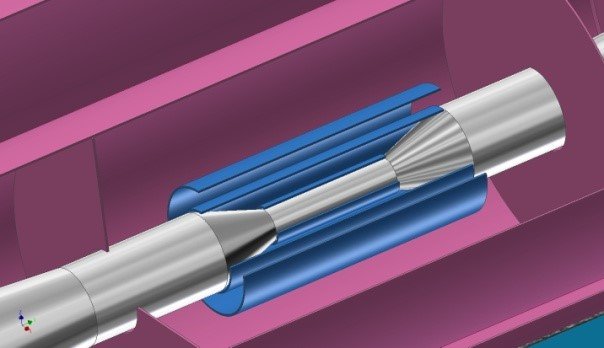
\includegraphics[scale=1.5]{Figures/Vertex/view_of_pixel.jpg}
	\caption{Schematic view of pixel detector (blue)}
	\label{fig:view}
\end{figure}


The layout of the vertex detector is summarized in Table \ref{tab:structure}. It is based on extensive simulation and technical studies from ILD. According to the fast simulation results (see sector 4), the impact parameter resolution can reach the requirement by using the single point resolutions provided in the table.
\begin{table}[!h]
	\centering
	\begin{tabular}{c|c|c|c|c|c}
		\hline
		\ & $R(mm)$ & $\arrowvert z \arrowvert(mm)$ & $\arrowvert cos \theta\arrowvert$ & $\sigma(um)$ & $Readout\ time(us)$\\
		\hline
		Layer 1 & 16 & 62.5 & 0.97 & 2.8 & 20 \\
		\hline
		Layer 2 & 18 & 62.5 & 0.96 & 2.8 & 20 \\
		\hline
		Layer 3 & 37 & 125.0 & 0.96 & 4 & 20 \\
		\hline
		Layer 4 & 39 & 125.0 & 0.95 & 4 & 20 \\
		\hline
		Layer 5 & 58 & 125.0 & 0.91 & 4 & 20 \\
		\hline
		Layer 6 & 60 & 125.0 & 0.90 & 4 & 20 \\
		\hline
	\end{tabular}
	\caption{Vertex detector parameters}
	\label{tab:structure}
\end{table}


\section{Detector performance studies}

The identification of heavy flavor jets through the displaced vertex of longlived beauty and charm hadrons has proven to be a crucial technique in previous experiments. For 240GeV operation charged particles carrying the lifetime information in the jets are often quite soft. Therefore, flavor tagging depends crucially on the precise reconstruction of low momentum (<10GeV) tracks, where multiple scattering dominates the performance. The main performance measure was the impact-parameter resolution projected in the transverse plane sigma(d0), which is closely linked to the flavour-tagging capability of the detectors. The goal is usually expressed in terms of the following parameterization of the transverse impact parameter resolution in a cylindrical vertex detector with uniform spatial resolution and material:
$$\Delta d_{0}[um]=a[um]\oplus\frac{b}{p(GeV)sin^{3/2}\theta},\ where\ the\ design\ value\ of\ ILD\ a = 5,\ b=10.$$


The vertex detector performance has been evaluated for the baseline configuration in full GEANT4 simulations as well as in fast LDT simulations \cite{xx2}. In addition, following the studies of CLIC \cite{dannheim2011layout}, the fast simulation setup was used for geometry optimization studies and to evaluate the sensitivity of the results on the chosen parameters. Assessing the impact of the detector geometries and material budgets on flavor-tagging performance requires dedicated full-simulation studies and will be subject of future R\&D.

\subsection{Performance of the Baseline Configurations}
The impact parameter resolution following from the single point resolutions provided in the table is displayed in figure \ref{fig:angle} as a function of the particle momentum, showing that the ambitious impact parameter resolution is achievable.
\begin{figure}[h!]
	\centering
	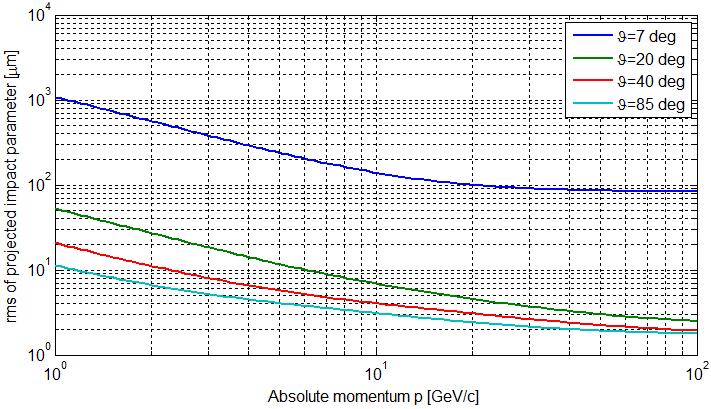
\includegraphics[scale=0.7]{Figures/Vertex/ipr_for_ang.png}
	\caption{Transverse impact-parameter resolutions for single muon events
		as a function of the momentum for different polar angles.}
	\label{fig:angle}
\end{figure}

\subsection{Material Budget}

The baseline designs include very small material budgets for the beam pipe as well as for the sensor layers and their support. To assess the sensitivity of the performance on the amount of material, the material budget for the beam pipe and for the detection layers of the vertex detector has been varied. The resulting transverse impact-parameter resolutions for low-momentum tracks are shown in figure  \ref{fig:material}. When increasing the thickness of the beam pipe by a factor of two, the resolution for tracks at theta= 90 degree increases by approximately 20\%. The same sensitivity is observed for doubling the material in all vertex layers.
\begin{figure}[h!]
	\centering
	\subfigure[] {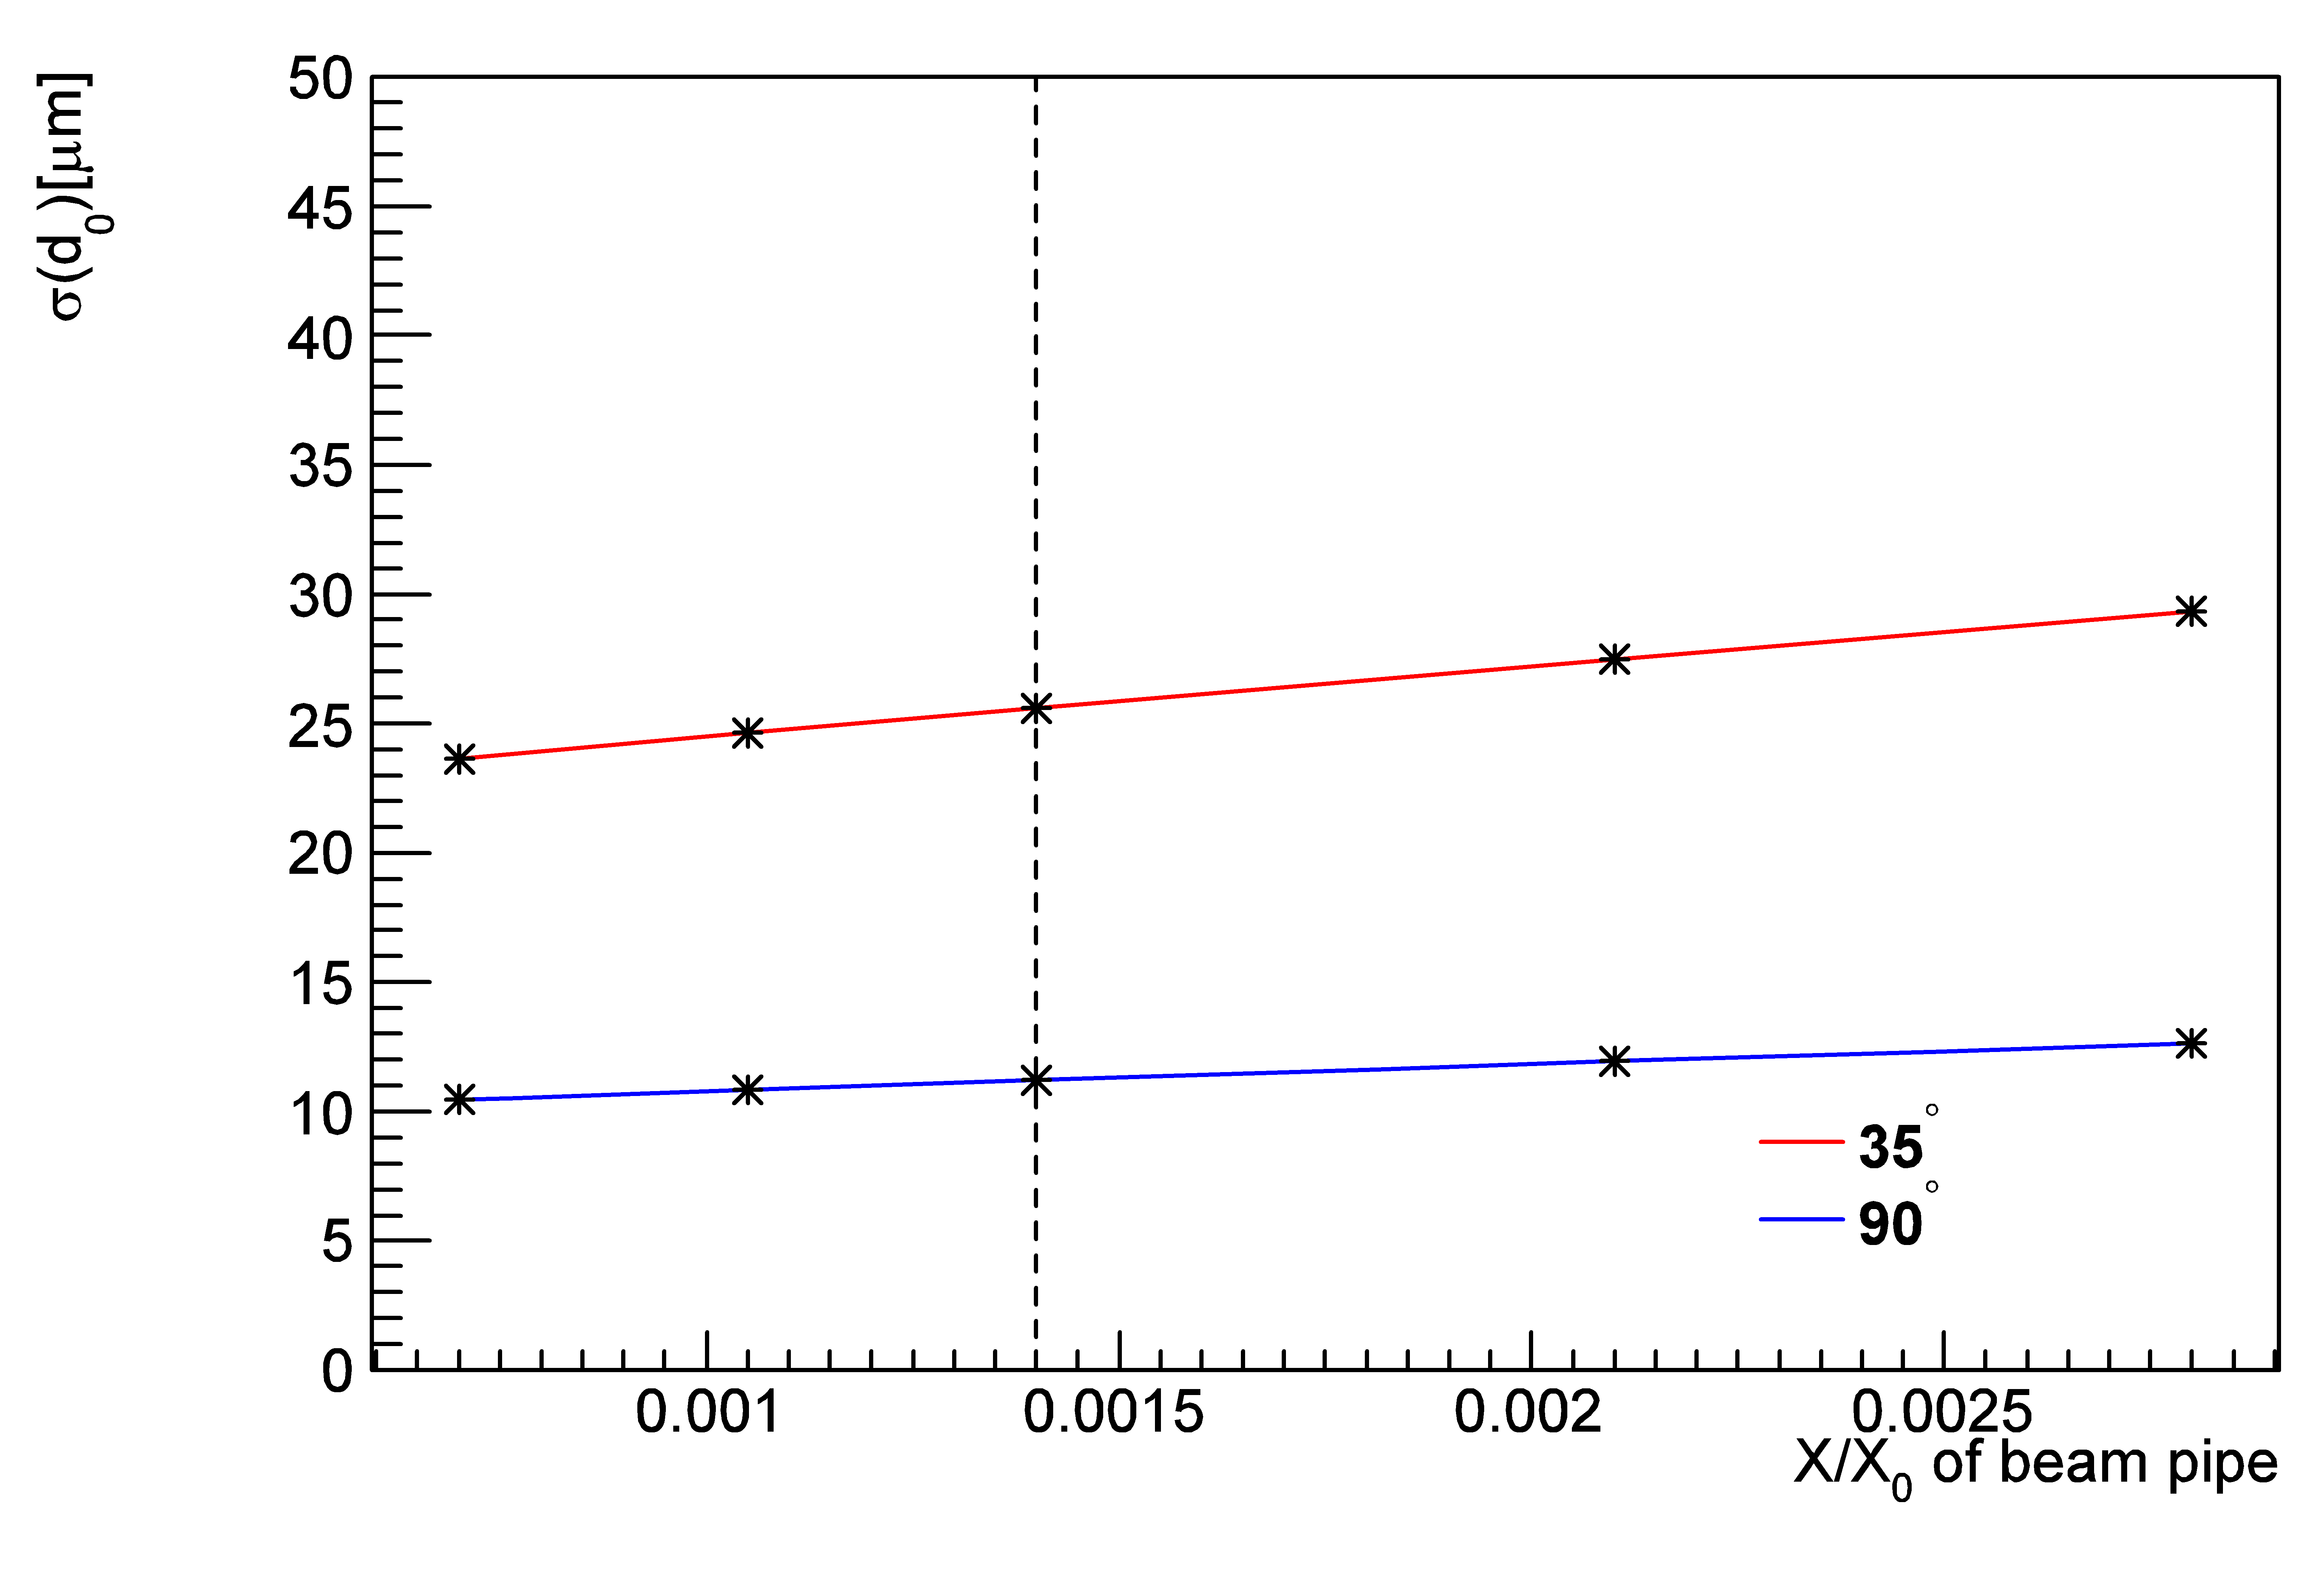
\includegraphics[height=2.2in,width=2.6in,angle=0]{Figures/Vertex/ipr_for_mb_1.png}}
	\subfigure[] {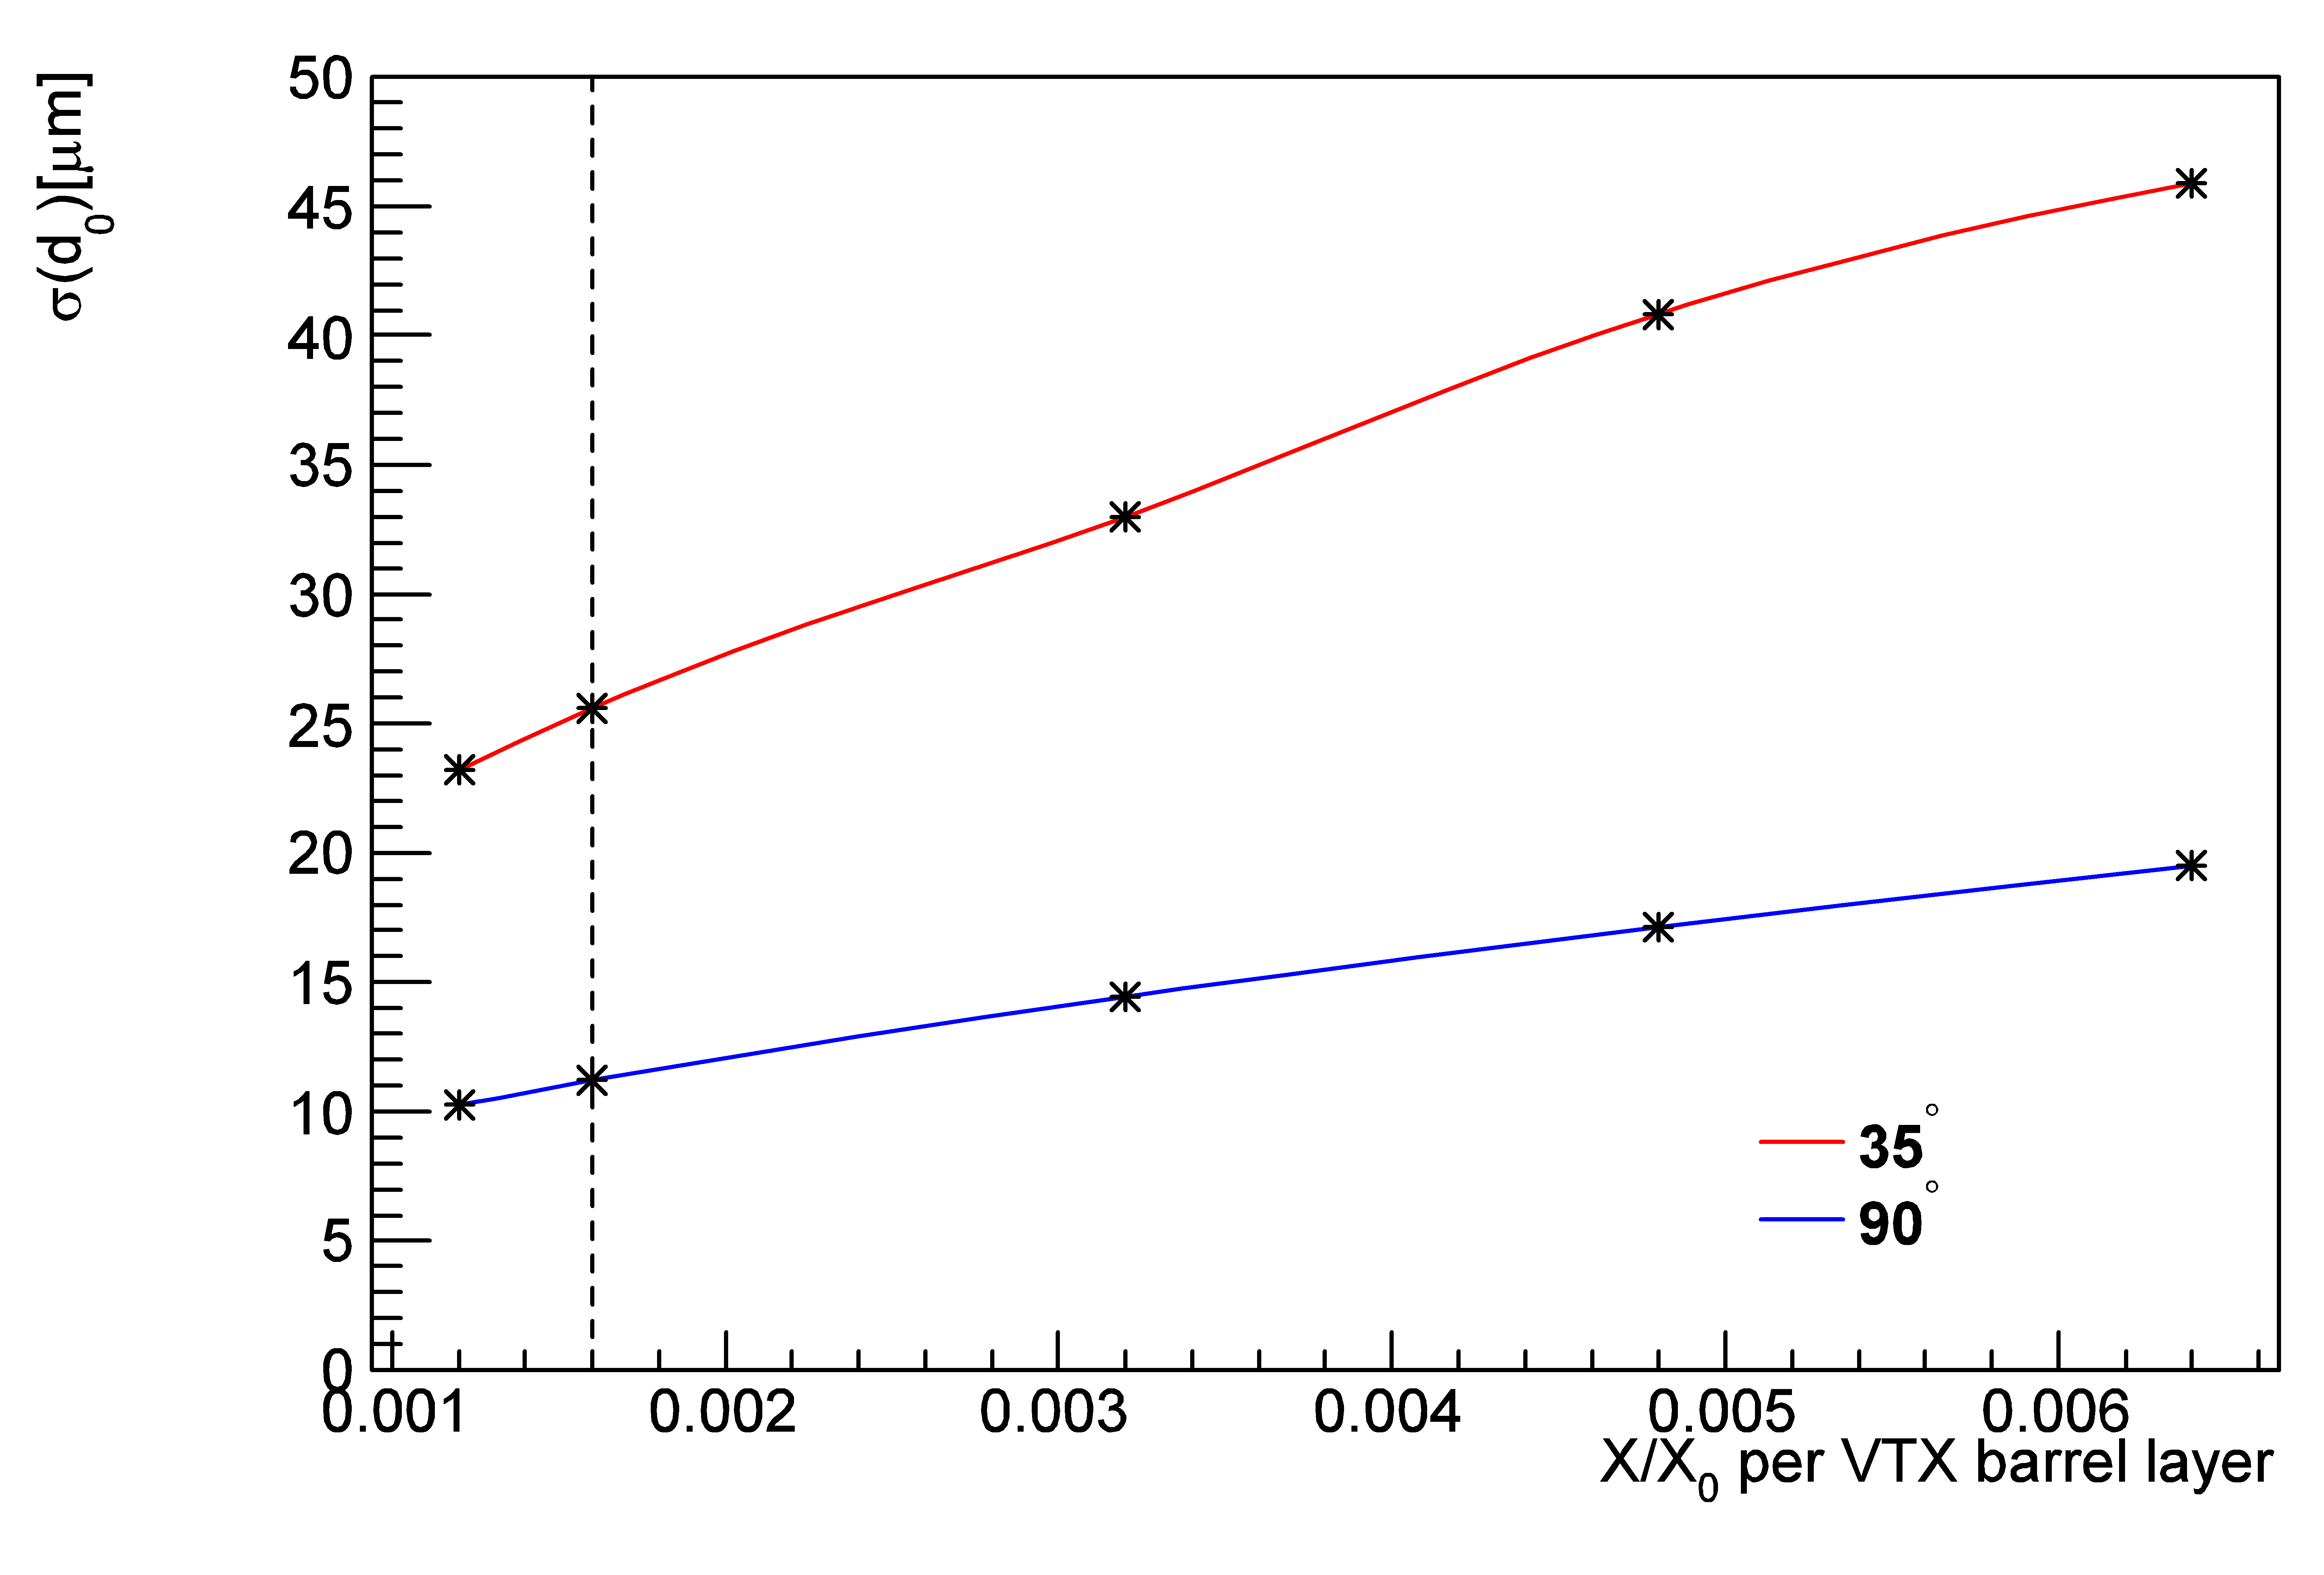
\includegraphics[height=2.2in,width=2.6in,angle=0]{Figures/Vertex/ipr_for_mb_2.png}}
	\caption{Transverse impact-parameter resolution of the CEPC vertex detector as function of the amount of material inside the beam pipe (a) and inside the vertex barrel double layers (b), as obtained from the fast LDT simulation. The results are shown for 1GeV tracks and for polar angles of theta = 35 degrees and of theta = 90 degrees. The material budget corresponding to the baseline configuration is indicated by dashed lines.}
	\label{fig:material}
\end{figure}

\subsection{Dependence on Single-Point Resolution}

The dependence of the transverse impact-parameter resolution on the pixel size was studied by varying the single-point resolution for the simulation of the vertex layers by +50\% w.r.t. the baseline values. The resulting resolutions for high and low track momenta as function of the polar angle theta are shown in figure \ref{fig:res}. The resolution for track momenta of 10GeV is found to change by approximately 30\% larger in the barrel region. Here they exceed the target value for the high-momentum limit of a ~= 5um for both pixel sizes, as expected from the corresponding single-point resolutions. For 1GeV, where multiple-scattering effects dominate, the corresponding variation of the transverse impact-parameter resolution is only 10\% larger. The target value for the multiple-scattering term of b~=10um is approximately reached for both pixel sizes. It should be noted, however, that the pixel size is also constrained by the background occupancies (see chapter MDI) and the ability to separate adjacent tracks in very dense jets in the presence of such backgrounds.
\begin{figure}[h!]
	\centering
	\subfigure[] {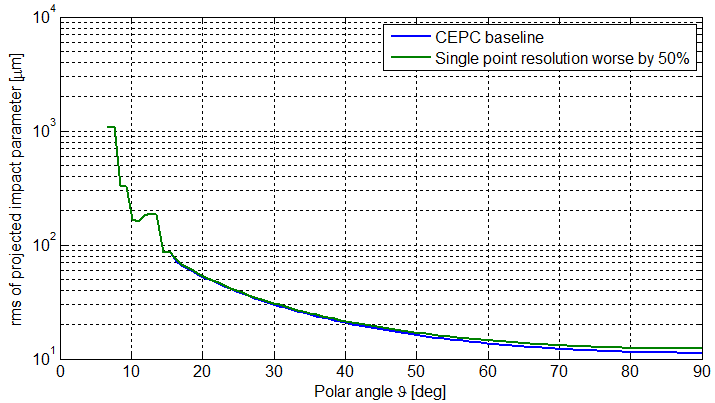
\includegraphics[height=2.2in,width=2.6in,angle=0]{Figures/Vertex/ipr_for_1.png}}
	\subfigure[] {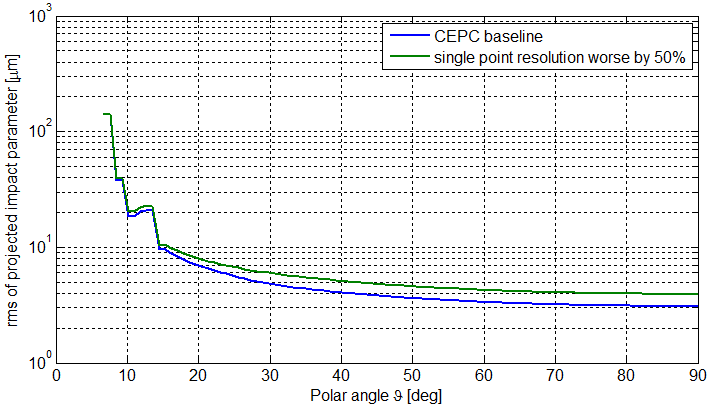
\includegraphics[height=2.2in,width=2.6in,angle=0]{Figures/Vertex/ipr_for_10.png}}
	\caption{Transverse impact-parameter resolution as function of the polar angle theta for different values of the single-point resolution of the CEPC barrel vertex detector, as obtained from the fast LDT simulation. Shown are the resolutions for 1 GeV tracks (a) and for 10 GeV tracks (b).}
	\label{fig:res}
\end{figure}

\subsection{Distance to IP}

The distance of the central beam pipe and barrel vertex layers to the IP was varied by the same amount for all layers of the CEPC vertex detector. Figure \ref{fig:distance} shows the resulting transverse impact-parameter resolutions at theta = 90 degrees as function of the momentum with different radial distance of the innermost barrel vertex layer to the IP. For low momentum tracks, the transverse impact-parameter resolution is proportional to the inner radius.
\begin{figure}[h!]
	\centering
	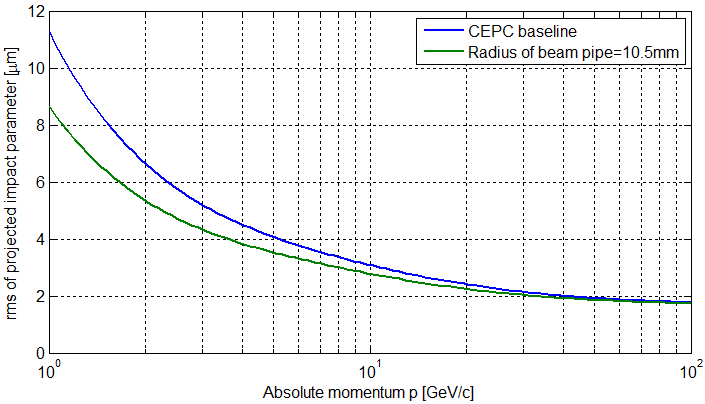
\includegraphics[scale=0.7]{Figures/Vertex/ipr_for_mom.png}
	\caption{Transverse impact-parameter resolution at theta= 90 degrees as a function of the momentum. Blue curve indicates the baseline configuration and the green curve indicates the configuration with the radius of beam pipe=10.5 mm.}
	\label{fig:distance}
\end{figure}

\section{Beam-induced Background in the Vertex Detector}

\section{Sensor Technology Options}

The history of silicon pixel vertex detector could be traced back to LEP era, when it was introduced in the DELPHI experiment \cite{andreazzadelphi}, and significant progress has been made over the last 20 years \cite{hartmann2009delphi}. There have been lots of R\&D efforts towards pixel sensors for vertex tracking in the future particle physics experiments \cite{battaglia2013r}, driven by track density, single point resolution and radiation level. 


As outlined in Section 2, the detector challenges include high IP resolution, low material budget, low occupancy and sufficient radiation tolerance (mild comparing to ILC but not necessarily easy to achieve). To fulfill these requirements of system level, the vertex must be based on sensor technologies which push for fine pitch, low power and fast readout. In the CEPC case it is a unique scenario that might be more requiring than previous applications. In the ILC\cite{Behnke_2013} and CLIC\cite{linssen2012physics}, for example, the power consumption is expected to be significantly reduced by choosing operation of power pulsing, but it is not practical for CEPC. Some other experiments such as the STAR\cite{contin2015maps}, BELLEII\cite{lacasta2014depfet} and ALICE upgrade\cite{abelev2014technical} do their readout continuously the same way the CEPC does. However, they require less in terms of IP resolution and material budget. A sensor technology that fits perfectly in needs of the CEPC does not exist. A few options are listed here for being either close to it or having outstanding potential.


The DEPFET has a unique feature that the main heat sources are located at the end of staves. As the thermal simulation of the BELLEII staves shown in figure \ref{fig:thermal}, 1W for sensitive area and another 1W for switcher located within the acceptance can be cooled by a gentle air flow, while the major heat of 16W in total for readout ASICs located out of acceptance can be removed by massive $CO_{2}$ cooling. The half stave for the BELLEII has achieved a low material budget of 0.21\% and a fast readout of 20us/frame. With a sensitive area of 64.4mm*12.5mm, it seems applicable as the inner most layers of the CEPC. A rough estimate results in 2.5W/ladder in sensitive area and 50us/frame readout speed due to finer pixel pitch required by the CEPC. It needs further investigation As the largest possible size of a half stave is limited to be inside a 6-inch wafer, the length of outer layers gets out of reach for the DEPFET.
\begin{figure}[h!]
	\centering
	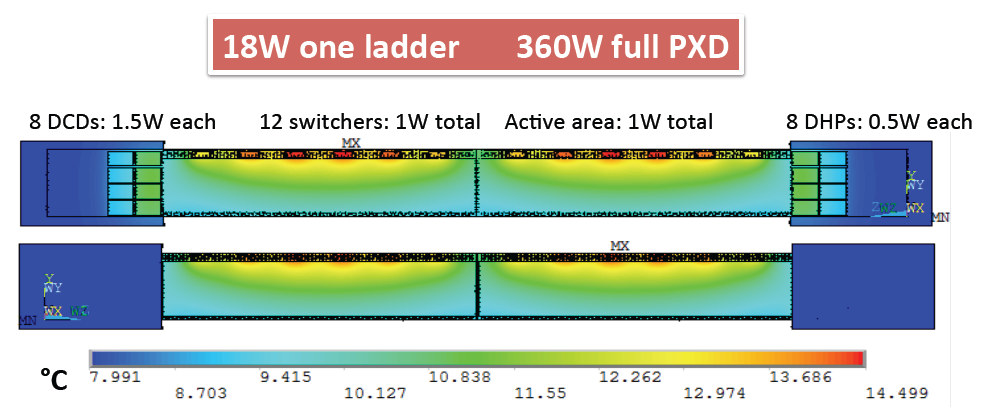
\includegraphics[scale=0.5]{Figures/Vertex/thermal_simu.png}
	\caption{Thermal simulation of the BELLEII staves}
	\label{fig:thermal}
\end{figure}


The HR-CMOS is gaining momentum from R\&Ds for the ALICE upgrade. Considering success of the MAPS (its predecessor) in the STAR and rapid progress achieved in the ALICE upgrade, HR-CMOS is possibly the most mature technology for an application like the CEPC. It has been approved to meet every single aspect of requirements of a CEPC-like detector. However, it is still challenging as to put all the specifications into a single chip. Intensive studies on circuit optimization (in-pixel discrimination) and innovative readout scheme (column sparsification) are underway. Pushing the power consumption down to $50mW/cm^2$ is a critical goal for application in the CEPC case.


The SOI is an option with great potential. The issue of coupling between sensor and circuit has been well understood and is addressed properly. There are a wide variety of applications in astrophysics\cite{nakashima2013development}, material science\cite{hatsui2013direct} and particle physics\cite{ONO2013266} which keep the MPW running steadily. This technology features fully depleted high resistive substrate, 0.2um full CMOS process and being apt to 3D integration. The IHEP group has been developing both chips with fine pitch and chips with complicated function for over 3 years. Making best use of the high quality sensor and the SOI CMOS process could lead to good S/N ratio, which benefits an optimum solution of low power and fast readout. Similar to the HR-CMOS, the upper limit of power consumption is set to 50mW/cm2.


The criteria of being able to cope with continuous colliding and to still remain low power distinguished the 3 sensor options out of other technologies on market. Both the Chronopixel proposed for SiD/ILC and the CLICpix for the CLIC, for example, consume large amount of current in pixel level and rely on power pulsing heavily. HV-CMOS\cite{peric2012active} is proposed more like a hybrid sensor and only minimum electronics on chip. The current R\&D efforts are focusing on ATLAS-alike architectures and are definitely not suitable for precise measurement on an electron-positron collider.

\section{Mechanics and Integration}

The design of the vertex detector is conceived as a barrel structure, including six concentric layers. The preliminary layout of each layer is shown in table \ref{tab:layout}. The range of the radii covered by the detector is from 16mm to 60mm. The length of layers 3 to 6 is 125cm, which is twice as long as the first two layers.
\begin{table}[!h]
	\centering
	\begin{tabular}{c c c}
		\hline
		No. of layer & radius (mm) & length (cm) \\
		\hline
		Layer 1 & 16 & 62.5 \\
		\hline
		Layer 2 & 18 & 62.5 \\
		\hline
		Layer 3 & 37 & 125.0 \\
		\hline
		Layer 4 & 39 & 125.0 \\
		\hline
		Layer 5 & 58 & 125.0 \\
		\hline
		Layer 6 & 60 & 125.0 \\
		\hline
	\end{tabular}
	\caption{The preliminary layout of each layer}
	\label{tab:layout}
\end{table}


The detector may be realized by 3 double-sided layers. Each double-sided layer is equipped with pixel chips on both sides, and has a common support frame. In the azimuthal direction, each layer is segmented in elements called ladders. The ladder, which extends over the whole length of the layer, is the basic building block of the detector. It contains all structural and functional components, such as chips, flex cable, support frame and cold plate if it is necessary. Pixel chips in a row are connected to flex cable by wire bonding or other bonding techniques, and then glued to the support frame, which is composed of low Z materials, such as carbon fiber and silicon carbide, providing stable mechanical support. The other side of the support frame is equipped with another pixel chips layer. 


The design of the ladders should take into account the specifications of the vertex detector. In order to reduce a small multiple Coulomb scattering contribution to the charged-track vertex resolution and control deformations from gravity and cooling forces for the sensors position stability, the ladder mechanical support must fulfill stringent requirements in terms of minimum material budget and highest stiffness. The ladder design of other experiments can be as references, such as STAR pixel detector (PXL), the upgrade of ALICE inner tracking system (ITS) and BELLEII pixel detector (PXD), especially ILD vertex system, which takes double-sided ladder as an alternative ladder design. 


The ladder mechanical support is inherently linked to the layout of the cooling system that will be adopted to remove the heat dissipated by the pixel sensors since the cooling system is integrated in the mechanical structure. The key point of the cooling system design of the vertex detector must balance the conflicting demands of efficient heat dissipation with a minimal material budget. So suitable cold plate, which is coupled with pixel sensors, with high thermal conductivity and low material budget should be taken into account in the ladder design. There are two main types of cooling methods in particle physics experiments, air cooling and active cooling. Table \ref{tab:cooling} gives a list of cooling methods and the corresponding material budget of each layer of the aforementioned experiments. The upgrade of ALICE ITS \cite{abelev2014technical} adopts water cooling with respect to a chips power dissipation value of 300mW/cm2. Polyimide cooling pipes fully filled with water are embedded in the cold plate. STAR- PXL \cite{wieman2009star} uses air cooling according to its chips power consumption of $170mW/cm^{2}$. For ILD \cite{Behnke_2013} vertex system, two different cooling options are considered, depending on the sensor technology. The sensors and SWITCHER chips of BELLE II PXD \cite{abeoctober} require air cooling, while active cooling will be used for readout chips on each end of the detector, which is out of the sensitive region of the detector. So for CEPC vertex detector, the suitable cooling method will be determined according to the sensor option and the power consumption.
\begin{table}[!h]
	\centering
	\begin{tabular}{c c c c}
		\hline
		Vertex detector & Power dissipation & Cooling method & Material budget \\
		& & & requirement/layer \\
		\hline
		Alice ITS & $300\ mW/cm^2$ & water & 0.3\% \\
		\hline
		STAR PXL & $170\ mW/cm^2$ & air &  0.39\% \\
		\hline
		ILD vertex & <$120 mW/cm^2$ (CPS and DEPFEET) & air or $N_2$ & 0.15\% \\
		& 35W inside cryostat (FPCCD) & two-phase $CO_2$ & \\
		\hline
		BELLEII PXD & 20W for sensor and SWITCHER & Air & 0.2\% \\
		& 180W on each end & $CO_2$ & \\
		\hline
	\end{tabular}
	\caption{Cooling method of the vertex detector in each experiment}
	\label{tab:cooling}
\end{table}


Simulation and module prototype studies should be carried out to find suitable designs that can meet requirements of stability, cooling and the performance of the vertex detector. 


For the design of the whole mechanical structure of the vertex detector, some criteria must be taken into account. Firstly, minimum material has to be used in the sensitive region to reduce multiple Coulomb scattering. Secondly, to ensure high accuracy in the relative position of the detector sensors and provide an accurate position of the detector with respect to the central tracker of TPC and the beam pipe, a mechanical connector or locating pin at each end of the ladder should be considered to allow the fixation and alignment of the ladder itself on the end rings. Thirdly, cooling system should be arranged reasonably to ensure stable heat dissipation. At last, to reduce the dead region caused by the boundary of each ladder, neighboring ladders should be partially superimposed. 


In addition, the main mechanical support structures of the vertex should also meet the requirements of the integration with the other detectors, such as time projection chamber (TPC) and forward tracking disks. 


\section{Critical R\&D}

As outlined above, the proposed vertex detector will be based on novel silicon pixel technologies, with low power consumption pixel sensor, and low-mass mechanical structure, to meet the stringent performance requirements of the experiment. Since the technologies are not mature enough at the moment, there still needs critical R\&D efforts to make them available for engineering construction. 

\subsection{Current R\&D activities}
\subsubsection{CMOS Pixel Sensor}
\subsubsection{SOI Pixel Sensor}

\subsection{Future R\&D}

\subsubsection{Pixel sensors with lower power consumption and higher readout speed}

From the view point of circuit design, readout speed and power consumption contradict to each other. However moving column-shared discriminators into individual pixel would benefit readout speed and power reduction simultaneously in a conventional rolling shutter scheme. More efficient readout schemes can be implemented by in-pixel discrimination and column-coding to avoid periodical polling through the entire pixel array. Much of the improvement and optimization at sensor level are related to such circuit design as mentioned above.

\subsubsection{Mechanical design and cooling}

Cooling, mechanical support and cabling within the acceptance are engineering challenges. In order to build ladders with discrete chips of HR-CMOS or SOI, light weight mechanical support and cabling are necessary with a material budget of less than 0.05\%/X0 each. As for DEPFET all-silicon staves, the total material budget is expected to be 0.15\%/X0. Manufacturing and assembling of those ladders/staves have to be verified. In addition, the vibration must be characterized carefully so as to obtain enough cooling capability and not degrade the IP resolution. In the case of DEPFET, additional $CO_{2}$ cooling has to be introduced to cool the hot spots of ASIC chips, which makes the system more complex.

\subsubsection{Sensor thinning}

Thinning sensors down to 50um has been demonstrated on MAPS chips/wafers, which does not require further process on the backside of chips/wafers. While both DEPFET and SOI require backside process after thinning. DEPFET for BELLEII was thinned to 75um in the sensitive area \cite{lacasta2014depfet} and is likely thinned to 50um without fundamental difficulty. SOI already achieved 110μm thickness without any adverse effect observed  \cite{xx18}. The reliability and yield after thinning to 50um have to be studied carefully.

\section{Summary}

The basic concepts in the ILD Vertex detector, including the pixel sensors' specifications required by IP resolution and radiation tolerance, the low-mass mechanical design, and the barrel geometry, are essentially adapted to the baseline design of CEPC Vertex detector. However, due to CEPC's continuous working mode, the R\&D is critically needed to reduce the sensor power consumption and charge collection time. Further, more detailed designs for mechanical supports and cooling, cabling, and power conversion are also necessary. Most of those issues could be learnt and improved from R\&D activities for the ILC detectors. 




\bibliographystyle{Style/atlasnote} %% plain.bst
\bibliography{Chapters/Vertex} %% bsample.bib


%% $Id$
%%%%%%%%%%%%%%%%%%%%%%%%%%%%%%%%%%%%%%%%%%%%%%%%%%%%%%%%%%%%%%%%%%%%%%%%
\chapter{The silicon tracker}
\label{Chapter:SiTracker}

As described in the PreCDR~\cite{cepc:preCDR-1}, the silicon tracker,
together with the vertex detector and the TPC, forms the complete
tracking system of CEPC. With sufficiently low material budget to
minimise the multi-scattering effect, the silicon tracker provides
additional high-precision hit points along trajectories of charged
particles, improving tracking efficiency and precision significantly.
In addition to complementary tracking, it also provides the following
functionalities:
\begin{itemize}
\item monitoring possible field distortion in the TPC,
\item contributing detector alignment,
\item separating events between bunch crossings with relative
  time-stamping.
\end{itemize}


\section{Baseline design}
%%______________________________________________________________________


\section{Sensor technologies and readout electronics}
%%______________________________________________________________________


\subsection{silicon micro-strip sensors}
%%______________________________________________________________________


\subsection{silicon pixel sensors}
%%______________________________________________________________________


\section{powering, cooling and mechanics}
%%______________________________________________________________________


\section{tracking performance}
%%______________________________________________________________________


\section{critial R\&D}
%%______________________________________________________________________


\bibliographystyle{Style/atlasnote}
\bibliography{Chapters/SiTracker}

\chapter{Tracking system}
\label{Chapter:TrackingSystem}


%This~\cite{cepc_website} is an example with plots, please edit ...
%
%\begin{figure}[h!]
%\centering
%\includegraphics[scale=0.36]{Figures/TrackingSystem/main_theme}
%\caption{A sketch of two of the central goals of the CEPC and SPPC. The CEPC will probe whether the Higgs is truly ``elementary", with a resolution up to a hundred times more powerful than the LHC. The SPPC will see, for the first time, a fundamentally new dynamical process --- the self-interaction of an elementary particle --- uniquely associated with the Higgs.}
%\label{fig:main_theme}
%\end{figure}
%
\section{TPC tracker detector}
In CEPC, the significant benchmark signals for higgs mass precise measurement is the ZH events where the Z decays to $\mu\mu$ or ee, whose branch ratios are both around 3.3$\%$ and momentum spreads from 20GeV to 80GeV. The inner tracking system for the CEPC detector should be sensitive in momentum measurement to charged particles, which transverse momentum ranged from 0 to 80GeV, with an accuracy compatible to the beam energy uncertainty of the accelerator.

The tracking system are expected to affect the flying of the tracks as less as possible, which require it to be as light as possible. The particle ID ability is one of the feasibility of the tracking system, however for such energetic tracks, the classic method, such as dE/dx, TOF are not reliable. The Cherenkov detector or Transition radiation detector can be used to combine with tracking for the both feasibilities, as what ATLAS experiment has done.To satisfy the requirement above, some candidate detectors can be considered. The multi-cell drift chamber based on wires is one of the candidates. The ions produced by the charged tracks drift inside a drifting cell configured by sensing wire and ground wires. The drift distance is quite small, which help to reduce the diffusion of the ions and achieve a good position resolution based on the drifting time. The advantage of this kind of detector is that the dead time is very short, however the wire tension require a very strong support structure of the detector which bring high mass in the forward region. The precise positioning of the wires are also complex in the mechanical manufacture. For the material budget of the DC, we see that a helium gas combining with wires achieve $1\%$ $X_0$, which is similar as the gas use in STAR TPC ($1.17\%$). However the inner skin or the out skin of the DC consume much more material, e.g. the inner skin of the MDC detector in BES3 corresponds to 0.45 $X_0$. Considering the cost, the performance and the complexity of the technique, TPC could be as our a good option for the tracker system.

Time Projection Chambers (TPCs) have been extensively studied and used in many fields, especially in particle physics experiments, including STAR and ALICE. Their low material budget and excellent pattern recognition capability make them ideal for three dimensional tracking and identification of charged particles. They are also the only type of electronically read gaseous detector delivering direct three-dimensional track information. However, there has always been a critical problem with TPCs, especially in high background conditions, the space charge distortion due to the accumulation of positive ions in the drift volume.

Due to their large mass, positive ions move slowly under the action of electric field in the drift volume of the TPC. The continuously superimposed ions in the drift volume of the TPC may affect the drift behaviour of electrons from a later track. The majority of ions inside the drift volume are backflowing ions from the amplification region of the TPC readout devices. It is thus of great importance to limit ion backflow (IBF) from the amplification region.

\subsection{Baseline design and mechanics}

\subsubsection{TPC detector geometry}
The expected TPC used in the CEPC detector works in a quite different environment than STAR and Alice experiment. The charge tracks multiplicity in CEPC is much less than STAR and Alice, however the momentum of the charged tracks in CEPC is much larger than STAR/Alice.
To precisely measure the momentum of the hard tracks, the tracker need to

\begin{enumerate}
\item	Sensitive to the track segment as long as possible.
\item	Stronger enough magnetic field for track bending.
\item	As good as possible position resolution of the track measurement.
\end{enumerate}

\begin{figure}[htbp]
\centering
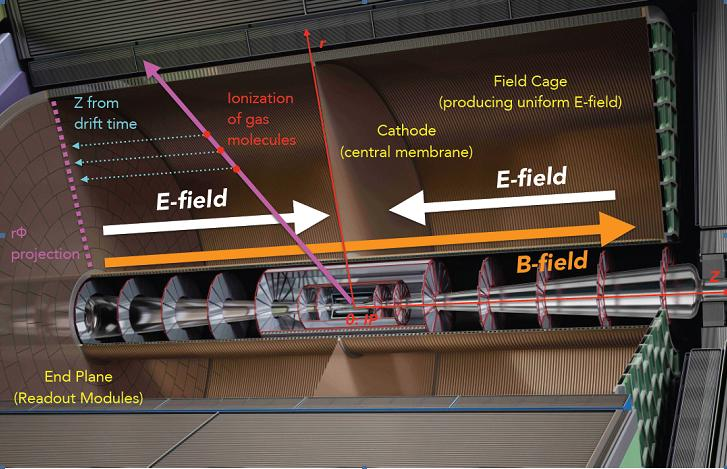
\includegraphics[width=0.75\textwidth]{figures/TrackingSystem/TPC_img5.jpg}
\caption{\label{fig:img5} Sketch of the TPC structure.}
\end{figure}

A large TPC construction has been approved to be possible in Alice/STAR. A 2-Tesla B-field has been used in ATLAS tracker and 4-Tesla B-field in CMS tracker, to measure the tracks which momentum is similar as expected in CEPC. The significant advantage for TPC is that the position resolution will be improved by strong B-field, as well, because the B-field helps to reduce the diffusion of the drifting electrons. The TPC is expected to be 460cm long and 360cm in diameter. The endcap is made of by GEM detector and divided into $2\!\times\!16$ divisions.  The schematic view of the end plate is shown below.

The mechanical structure of the TPC consists of a field cage, which is made with advanced composite materials, and two readout end-plates that are self-contained including the gas amplification, readout electronics, supply voltage, and cooling. It will be challenging to design and build the TPC support structure with relatively light material, and at the same time very rigid. It is required to maintain accuracy, robustness in all directions, and stability over long time periods. As the field cage is not strong enough due to the limited material budget, the end-plates become the only choice, where the support structure connects to. In current stage of design, how the TPC end-plate should be supported is not fixed yet. A promising solution is to suspend from the solenoid, in which a number of spokes run radically along the faces of the calorimeter to the TPC end-plates. Bearing is not the most challenging issue. Main efforts should be put on the system accessibility and robustness against various accidental movements, especially in the longitudinal direction. It is not decided yet in current stage design, but the inner and outer silicon trackers might be supported by the TPC field cage. Although with no severe conceptual issues, this additional load requires a stiffer structure and additional material budget.

In addition, the choice of supporting material is also limited by other requirements. It should be non-magnetic, vibration absorbing, with low thermal-expansion coefficient, and the ability to achieve a position accuracy of 100~$\mu$m level. Currently the carbon fibre enforced composite is the leading candidate of consideration.

\begin{enumerate}

\item Chamber

Large-scale TPC's chamber have been successfully employed in several collider experiments. TPC chambers are typically cylindrical and operate under the atmospheric pressure with the working gas filled inside. Chambers in high magnetic field close to the centre of the magnet, usually have a higher occupancy due to the curling low-energy tracks. Access for cables and services is limited in this region. Hence the material budget of stations inside the magnet is kept as low as possible. In the active area, the added the material due to the filled gas should be less than 1\%$X_0$.

The chambers are attached to the end-plate from the inside to minimise the dead area between neighbouring chambers. Special mounting technique is required to allow rotation and tilting of the chambers. It will be even more challenging to mount and support the CEPC TPC chambers of larger size.



\item  Field cage

The CEPC TPC detector will be a large cylinder with an outer diameter of 3.6~m and a total length about 4.7~m. Lightweight cylindrical inner and outer composite walls hold field and forming strips, which are attached to a resistor divider chain network. The resistors must be no-magnetic. A central cathode will be held at approximately 50~kV when the drift field is 300~V/cm, with the end-plates and the other outer surfaces of the TPC at ground potential. Therefore the composite walls must self-stand the large potential of the central cathode. The mirror narrow strips will be arranged between the inner and outer walls to keep the electron field uniform in over the whole active TPC volume.



\item  End-plate

To obtain high position resolution, every end-plate is subdivided into many independent MPGD detector modules (Thin GEM or Resistive Micromegas detector), which can provide nearly full coverage of the end-plate. Power cables, electronic connectors, cooling pipes, PCB boards and support brackets wall are also mounted on the end-plate.

In case the detector modules are damaged by the discharge or spark, they can be replaced and the end-plate should be kept stable during the replacement. In addition, the end-plate needs to built from lightweight material, not compromise the jet energy resolution in the forward region, but should be still sufficiently rigid to achieve stable positioning of the detector modules with a position accuracy better than 50~$\mu$m.The material budget of the mechanical structure accounts for 8\%$X_0$. Additional materials for the readout planes, front-end electronics and cooling are estimated to be 7\%$X_0$, and power cables and the connector up to 10\%$X_0$.
\end{enumerate}

\subsubsection{Operation gas and high voltage}
\begin{figure}[htbp]
\centering
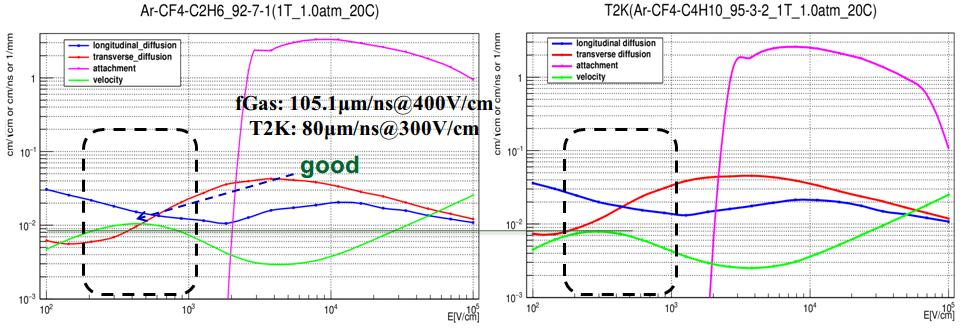
\includegraphics[width=0.98\textwidth]{figures/TrackingSystem/TPC_gas_vol.jpg}
\caption{\label{fig:gas_vol} The drift velocity in different gas mixture.}
\end{figure}


In given the working gas and the electric field, the drift velocity of electron could be determined with Eq.~\ref{eq:gas:1}

\begin{equation}
\label{eq:gas:1}
\mu_e=f(\frac{E}{P})
\end{equation}

\noindent where $E$ denotes the electric field vector, $P$ the gas pressure and $\mu_e$ the electron drift velocity. After reaching saturation (nearly maximum), the electron drift velocity depends slightly on the electric field. Fig.~\ref{fig:gas_vol} shows that the drift velocity obtained in different mixture gases. For the CEPC TPC detector, it is required to be sensitive to as long as possible track segment. The working gas should be selected in such way to achieve high velocity in low drift field to lower the high voltage in all of the drift length, and small transverse diffusion in the magnetic field to decrease the electron cluster size on the readout pads.


The gas mixture of Ar/CF$_4$/iC$_4$H$_{10}$ (95\%/3\%/2\%) have been used for the Large Prototype of TPC Detector for the ILD TPC and the TPC chamber for the T2K experiment. The saturated drift velocity of the mixed gas reaches nearly 8~cm/$\mu$s in a drift field of ~300~V/cm.  In addition, the gas has a large parameter of $\omega\tau$ (same as the Eq.~\ref{eq:gas:1})  and transverse diffusion coefficient of 30~$\mu$m/$\sqrt{\mathrm{cm}}$ in the drift field of 300~V/cm. In the $B$-field, a reasonable transverse diffusion coefficient could be realised at 100~V/cm of the drift field. The bunch spacing at the CEPC is $\sim 3.6~\mu$s. The working gas has an higher saturated drift velocity than the T2K mixed gas should be considered. In addition, the gas amplification needs to achieve approximately 6000 and the signal attenuation of the electron attachment should be kept below $1\%/m$.
\subsubsection{Electronics readout for TPC}

TBD

\subsection{Simulation and estimation for the key issues}
\subsubsection{Occupancy requirement of Higgs and Z pole run}

Using an sample of 9 thousand fully simulated $Z\to qq$ events at center of mass energy of $91. 2$ GeV, we studied the voxel occupancy and the local charge density of the CEPC TPC at $Z$ pole operation for future circular electron positron colliders, with an instant luminosity of $2\times 10^{34}$ to $2\times 10^{36}$ $cm^{-2}$ $s^{-1}$.

\begin{figure}[htbp]
\centering
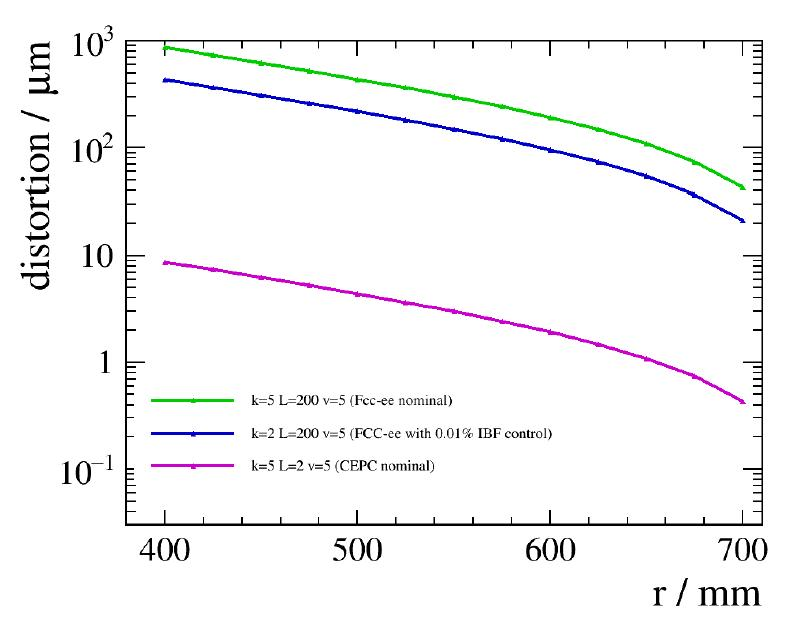
\includegraphics[width=0.70\textwidth]{figures/TrackingSystem/distortion.jpg}
\caption{\label{fig:distortion} Distortion as a function of electron initial r position with different parameters.}
\end{figure}


Given the fact that the beam bunch is evenly distributed along the accelerator circumference,
the voxel occupancy is extremely low ($1.4\times 10^{-5}/1.4\times 10^{-7}$ for the inner most layer and $3.4 \times 10^{-6}/3.4 \times 10^{-8}$ for average) and poses no pressure for the TPC usage. The distortion on TPC hit positions induced by the ion charges is estimated with dedicated
program and calculation. At instant luminosity of $1 \times 10^{36}$ and an ionback flow control of percent level, the distortion can be as large as 10 mm at the inner most TPC layer at the CEPC conceptual detector geometry, which is two orders of magnitude larger than the intrinsic TPC spatial resolution.
A few approaches are proposed to reduce the effects caused by distortion:
\begin{enumerate}
\item Ion back flow control technology; the ion back flow should be controlled to per mille level, in other word, only $1-10$ back flow ions is allowed for each primary ionization.
\item Dedicated distortion correction algorithm, for the inner most layers, which should result in a mitigation of the hit position distortion by 1 order of magnitude.
\item Adequate track finding algorithm that could link the TPC track fragments to vertex tracks at high efficiency and purity.
\end{enumerate}

Taking all of these approaches account, the distortion can be mitigated by approximately 2
orders of magnitude. To conclude, the pad occupancy and distortion stress no pressure to CEPC
and if the above items can be achieved, the usage of TPC is also a feasible option at FCC-ee.

\subsubsection{Distortion of Ions backflow in drift length}
Early TPCs were equipped with multi-wire tional chambers (MWPCs) as gas amplification devices. The IBF ratio in a standard MWPC is $30-40\%$ so a gating grid is essential to prevent ions from  reaching the drift volume. In the presence of a trigger, the gating grid switches to the open state to allow ionization electrons to travel into the gas amplification region.
After a maximum drift time of about 100 $\mu s$ (depending on the drift length, electric field and gas mixture), the gating grid is closed to prevent positive ions from drifting back into the drift volume. Since it must remain closed until the ions have been collected on the grid wires, the ionization electrons are also blocked during this time and the dead time consequently increases.

Triggered operation of a gating grid will therefore lead to loss of data. Thus, the TPC at the proposed circular collider will have to be operated continuously and the backflow of ions must be minimized without the use of a gating grid.

\begin{figure}[htbp]
\centering
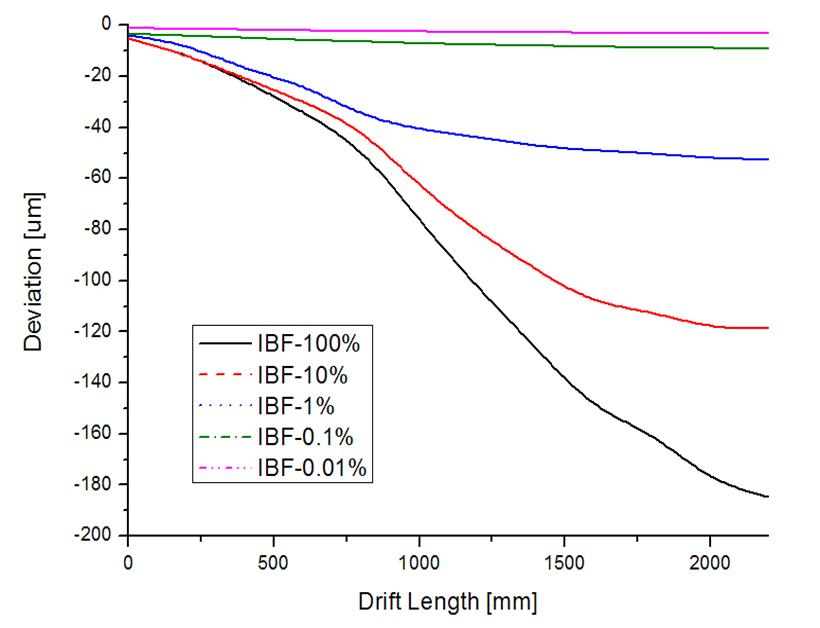
\includegraphics[width=0.65\textwidth]{figures/TrackingSystem/TPC_distortion.jpg}
\caption{\label{fig:TPC_distortion} Evaluation of track distortions due to space charge effects of positive ions.}
\end{figure}



\subsection{feasibility study of the TPC detector module and calibration system}
\subsubsection{Continuous IBF detector module}

\begin{figure}[htbp]
\centering
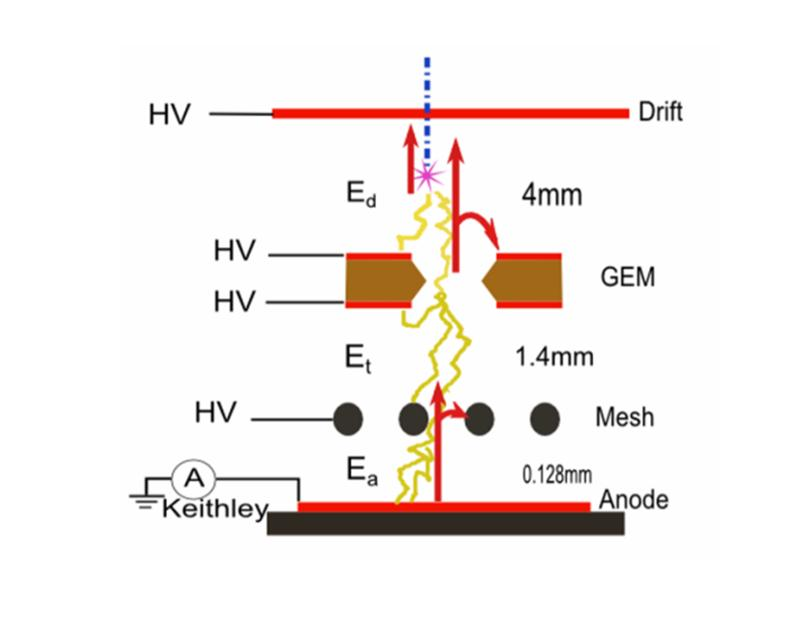
\includegraphics[width=0.65\textwidth]{figures/TrackingSystem/TPC_IBF_det.jpg}
\caption{\label{fig:TPC_IBF_det} Schematic diagram of the detector module.}
\end{figure}

TPC readout with micro-pattern gaseous detectors (MPGDs), especially Gas Electron Multipliers (GEM)and micro-mesh gaseous structures (Micromegas), is very attractive, because the IBF of those detectors is intrinsically low, usually around a few percent. GEM detectors have been extensively proved in the last decade to be the prime candidate, as they offer excellent results for spatial resolution and low IBF. Several GEM foils can be cascaded, allowing multilayer GEM detectors to be operated at an overall gas gain above $10^4$ in the presence of highly ionized particles. Micromegas is another kind of MPGD that is likely to be used as endcap detectors for the TPC readout. It is a parallel plate device, composed of a very thin metallic micromesh which
separates the detector region into drift and amplification volumes. The IBF of this detector is equal to the inverse of the field ratio between the amplification and the drift electric fields. Low IBF therefore favours high gain. However, high gain will make it particularly vulnerable
to sparking. The idea of combining GEM with Micromegas was first proposed with the goal of reducing the spark rate of Micromegas detectors. Preamplification using GEMa also extends the maximum achievable gain, so there have also been studies on gaseous photomultipliers with this hybrid configuration.

\begin{figure}[htbp]
\centering
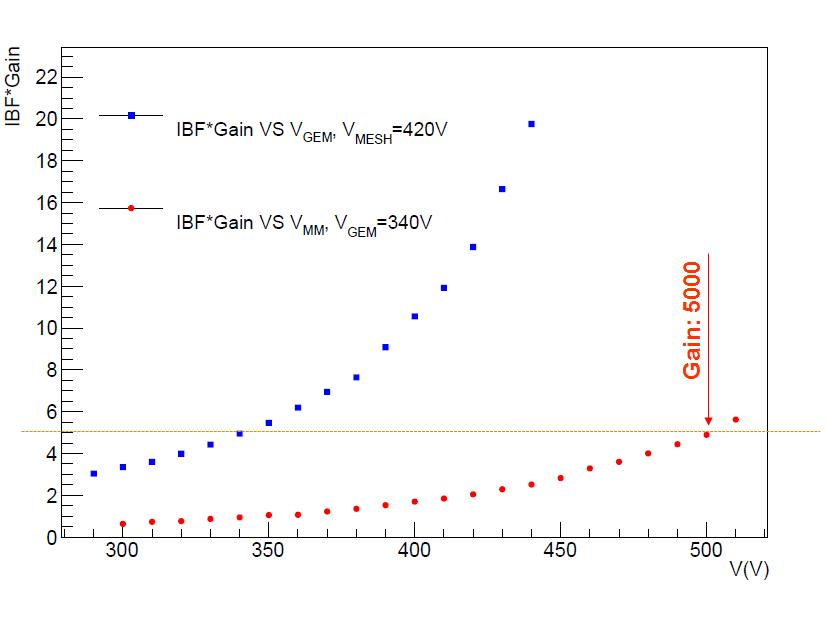
\includegraphics[width=0.80\textwidth]{figures/TrackingSystem/TPC_IBF_dig.jpg}
\caption{\label{fig:TPC_IBF_dig} Result of the IBF TPC detector module.}
\end{figure}

To fulfill the physics goals of the future circular collider, a TPC with excellent performance is required. MPGDs with outstanding single-point accuracy and excellent multi-track resolution are needed. We have proposed and investigated the performance of a novel configuration detector module: a combination of GEM and a Micromegas. The detector will be called GEM-MM for
short throughout this paper. The aim of this study is to suppress IBF continually by eliminating the gating grid. The design concept and some preliminary results of the detector module are described as following.

A new concept of avalanche ion backflow reduction for a future MPGD readout based TPC, and a prototype has been developed. It is a hybrid structure with one GEM foil cascaded above the Micromegas detector. Tests of this detector have been carried out with an 55Fe X-ray source
in $Ar/CO_2(90/10)$ gas mixture. The preamplification effect of GEM foil has been demonstrated in the energy spectrum measurement. With the novel hybrid structure, the effective gain of the GEM can be measured even when it is relatively low. The energy resolution of this hybrid structure gaseous detector is measured to be $27\%$(FWHM). The gain properties of this device were measured. A gain up to about 5000 can be achieved without any obvious discharge behaviour. The currents on the anode and drift cathode were measured precisely with an electro-meter. Out experimental measurements show that IBF can be reduced down to $0.19\%$ at a gain of about $5000$.

\subsubsection{Laser calibration and alignment system}
\begin{figure}[htbp]
\centering
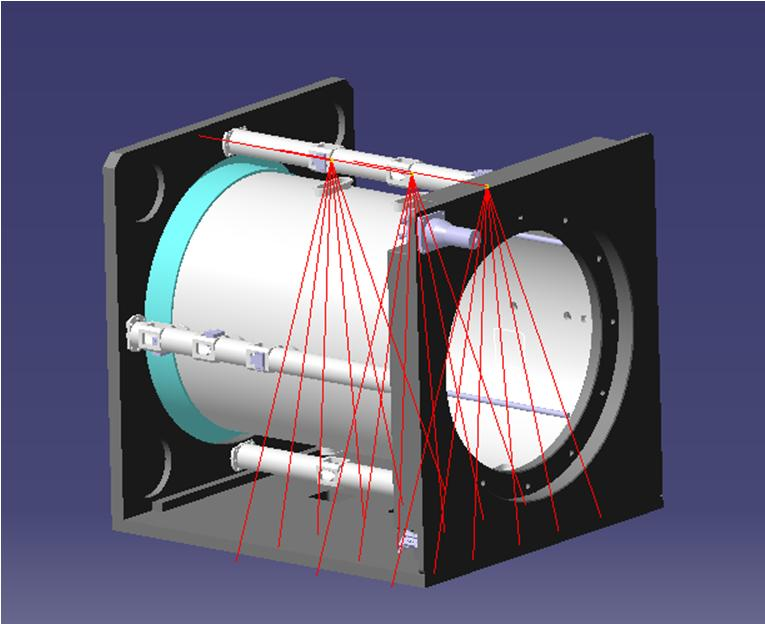
\includegraphics[width=0.80\textwidth]{figures/TrackingSystem/TPC_laser_dig.jpg}
\caption{\label{fig:TPC_laser_dig} Schematic diagram of the detector module with the laser system.}
\end{figure}


\section{Full-silicon tracker detector}
The design concepts for the tracking system at CEPC are similar to the ones studied for ILC~\cite{Adolphsen:2013kya,Behnke:2013lya},
which are required to provide excellent tracking efficiency and precision over a wide range of momenta for charged particles from the 
interaction point as well as from the decay of secondary particles. The tracking system must be built with minimal
material to preserve the momentum resolution and being covered hermetically down to the dip angle of 
$|cos\theta|<0.992$ from the beam pipe. There are two design options for ILC detectors, the large TPC+Silicon detector (ILD) and 
the compact full-silicon detector (SID), with very different approaches to achieve the same performances. 
The full-silicon tracker offers a well known technology that provides excellent space point resolution and granularity to 
cope track separation in dense jets and hits from the high luminosity beam related background. The drawbacks include the 
relative high materia density within the tracking system, less redundancy, and limited dE/dx measurements. 
Nevertheless, the purpose of this study is to demonstrate that the full-silicon tracking concept is a viable option for CEPC.

For designing a full-silicon tracker, we use the same detector boundary conditions considered in the CEPC v\_4
detector, which are summarized in the following,
\begin{itemize}
 \item the solenoid B field is set to 3~Tesla,
 \item the tracking envolope consists of a cylinder with a radius of 1.83~m and a length of 4.6~m,
 \item the tracker covers down to 7.25 degree from the beam pipe,
 \item the Be beam pipe has a radius of 1.45~cm and 14~cm long.
\end{itemize}

\subsection{Full silicon tracker layout} 
The ILD-like detector relies on a mixture of Time Projection Chamber (TPC) and silicon tracking system. However, the 
tracker could be converted using full silicon if the TPC is replaced with additional silicon stereo-strip layers (SIT) 
in the central region with disks of silicon stereo-strip detectors (FTD) on each side. 
In this design, the outer tracking system consists of a full-silicon tracker arranged as a set of six nested SIT layers in the central 
region with five FTD strip endcap disks on each side as shown in Fig.~\ref{fig:fullsigeom}. Details for design of 
SIT and FTD detectors can be found in the discussion of CEPC-ILD design~\cite{cepcILD} and
 we will use the same module design to build a full silicon detector as CEPC-SID. The pixel vertex detector (VTX) is kept the same as 
in CEPC v\_4.  
     
This new proposed tracking system provides at least 11 precisely measured points for all tracks down to a polar angle of about 15 degree and 
at least 7 measured points down to a polar angle of about 7.25 degree, as shown in Fig.~\ref{fig:fullnhit}. With three double pixel layers 
and forward disks covering a wide of polar angle, they are capable of providing excellent tracking on their own. 
The outer tracker adds additional track-finding constrains at large radii where hit density is low while improving the momentum 
measurement over a large level arm with excellent hit resolution in the transverse plane.

Alternatively, we could optimize the design of ILC-SID detector for CEPC by enlarging the outer silicon strip layers
to fulfil the space up to a radius of 1.83~m and z at $\pm$ 2.3~m in order to achieve comparable momentum resolution using
a lower solenoid B filed of 3~Tesla as shown in Fig~\ref{fig:fullsigeom}. The pixel detectors again are kept the same 
as in the ILC-SID design.  We will label this option as ``SIDB'', which provides an independent cross check on the tracking performance
using a full-silicon tracker. The number of expected hits on the track from SIDB is also shown in Fig.~\ref{fig:fullnhit}.  

Table~\ref{tab:fullsistrips} summarizes the geometry parameters of the proposed outer strip silicon trackers for CEPC between two full silicon 
options.

\begin{figure}[hbtp]
\begin{center}
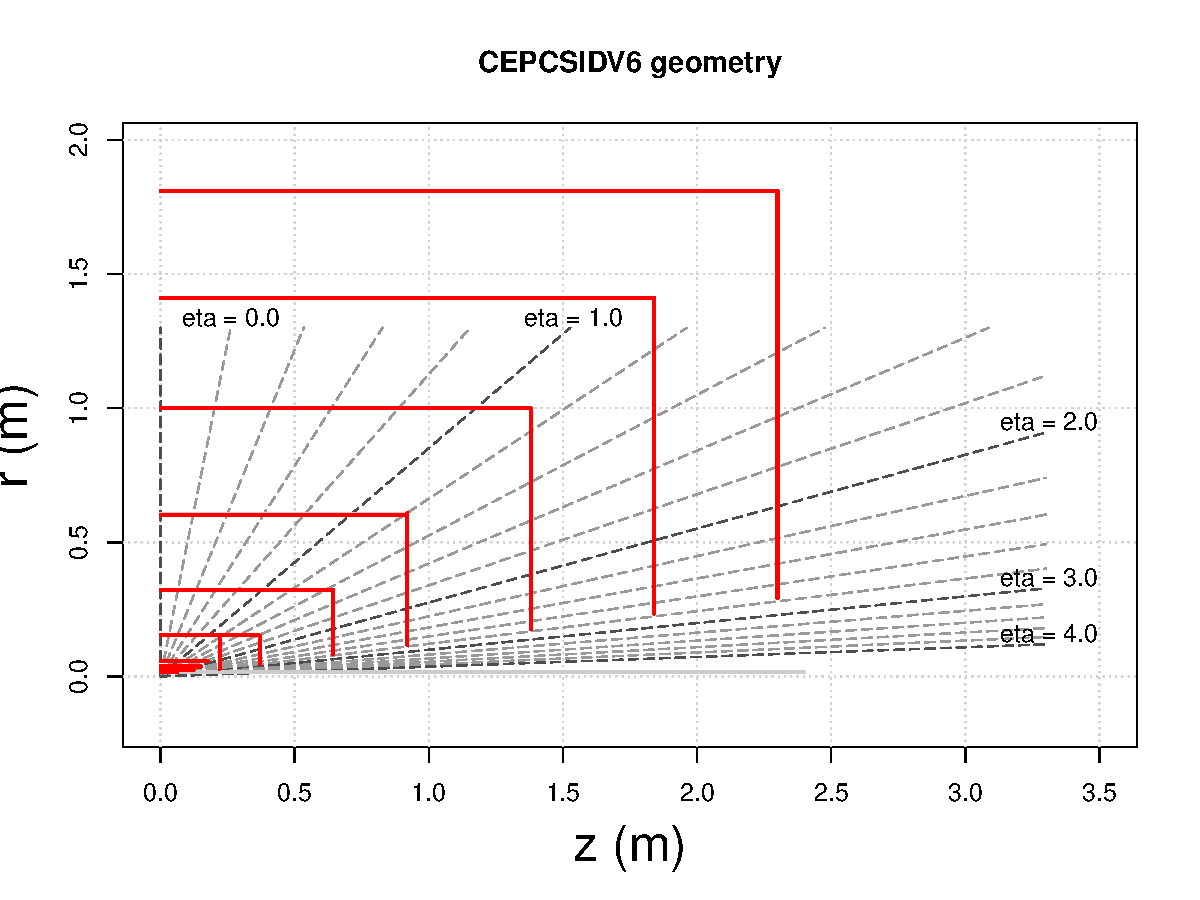
\includegraphics[width=0.32\textheight,keepaspectratio]{Figures/TrackingSystem/FullSilicon/Step1_CEPCSIDV6__geom_R.pdf}
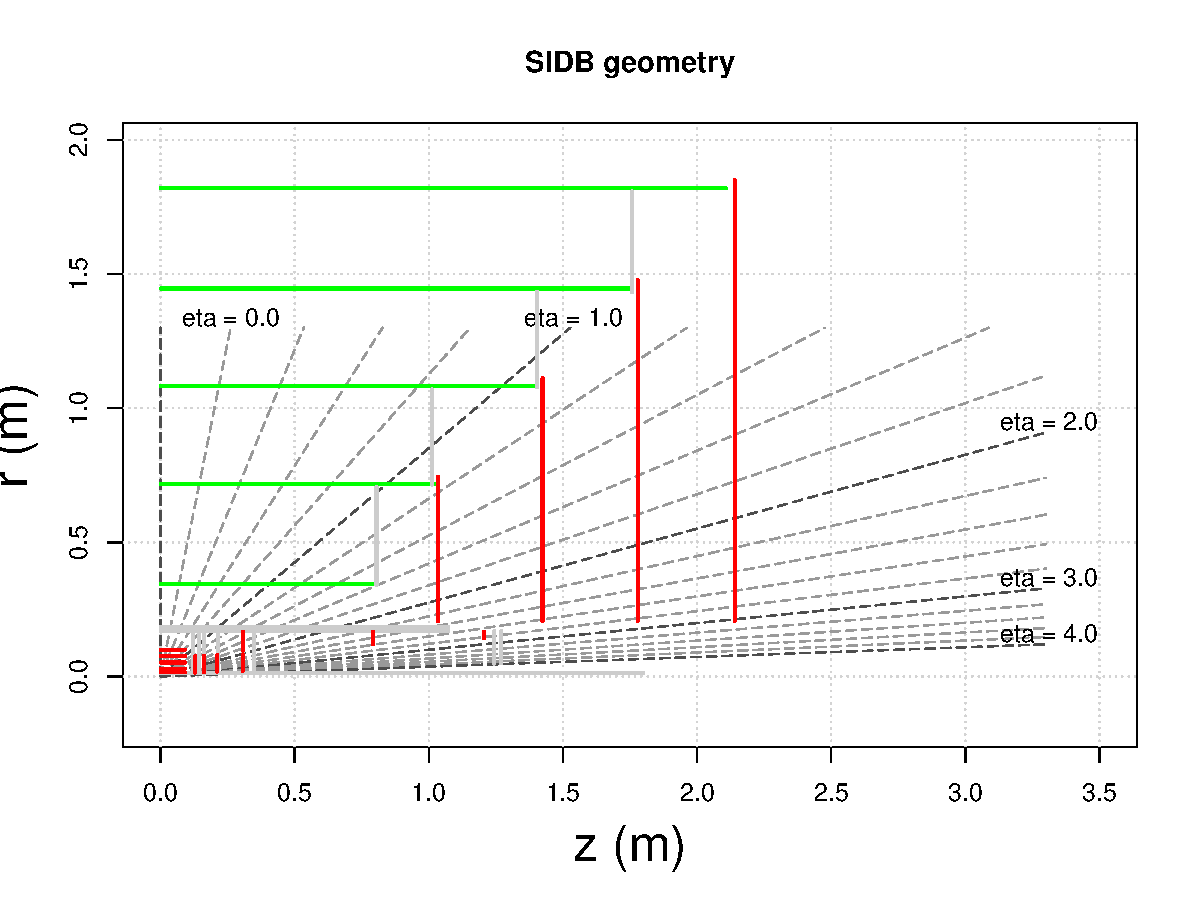
\includegraphics[width=0.32\textheight,keepaspectratio]{Figures/TrackingSystem/FullSilicon/Step1_SIDBig__geom_R.pdf}
\caption{The R-Z view of the full silicon tracker proposed for CEPC (left) and the enlarged version of SID design (right).\label{fig:fullsigeom}}
\end{center}
\end{figure}

\begin{figure}[hbtp]
\begin{center}
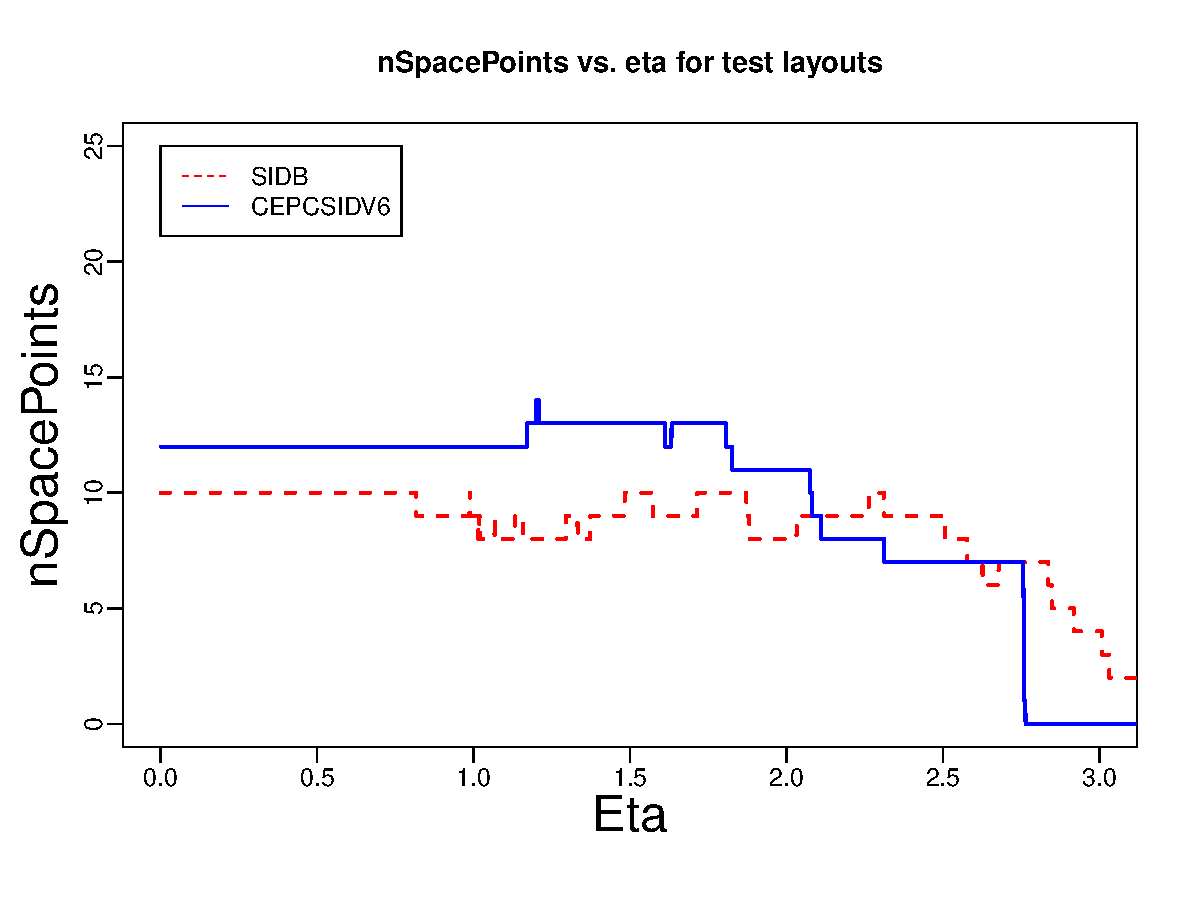
\includegraphics[width=0.45\textheight,keepaspectratio]{Figures/TrackingSystem/FullSilicon/Overlay_nHvsetaZ_R.pdf}
\caption{The number of expected hits are shown as function of track pesuro-rapadity.\label{fig:fullnhit}}
\end{center}
\end{figure}

\begin{table}[htb]
\caption{ The proposed geometry parameters for the outer strip barrel layers and disks,  where D and S stand for 
double and single-strip layer.}
\begin{center}
\begin{tabular}{|c|c|c|c|c|c|c|c|c|} \hline\hline
        & \multicolumn{4}{|c|}{CEPC-SID}          & \multicolumn{4}{|c|}{SIDB} \\ \hline 
Barrel  & \multicolumn{2}{|c|}{R (m)} & $\pm$z (m) & Type &  \multicolumn{2}{|c|}{R (m)} & $\pm$z (m) & Type  \\ \hline 
layer 0 & \multicolumn{2}{|c|}{0.153} & 0.368 & D  & \multicolumn{2}{|c|}{0.344} & 0.793 & S  \\  
layer 1 & \multicolumn{2}{|c|}{0.321} & 0.644 & D  & \multicolumn{2}{|c|}{0.718} & 1.029 & S  \\ 
layer 2 & \multicolumn{2}{|c|}{0.603} & 0.920 & D  & \multicolumn{2}{|c|}{1.082} & 1.391 & S  \\ 
layer 3 & \multicolumn{2}{|c|}{1.000} & 1.380 & D  & \multicolumn{2}{|c|}{1.446} & 1.746 & S  \\
layer 4 & \multicolumn{2}{|c|}{1.410} & 1.840 & D  & \multicolumn{2}{|c|}{1.820} & 2.107 & S  \\\hline 
layer 5 & \multicolumn{2}{|c|}{1.811} & 2.300 & D  & \multicolumn{4}{|c|}{} \\ \hline 
Endcap  & $R_{in}$ (m) & $R_{out}$ (m) & $\pm$z (m) & Type & $R_{in}$ (m) & $R_{out}$ (m) & $\pm$z (m) & Type \\ \hline 
Disk 0  & 0.082 & 0.321 & 0.644 & D & 0.207 & 0.744 & 1.034 & D \\
Disk 1  & 0.117 & 0.610 & 0.920 & D & 0.207 & 1.111 & 1.424 & D \\
Disk 2  & 0.176 & 1.000 & 1.380 & D & 0.207 & 1.477 & 1.779 & D \\
Disk 3  & 0.234 & 1.410 & 1.840 & D & 0.207 & 1.852 & 2.140 & D \\ \hline
Disk 4  & 0.293 & 1.811 & 2.300 & D & \multicolumn{4}{|c|}{} \\ \hline
\hline\hline
\end{tabular}
\end{center}
\label{tab:fullsistrips}
\end{table}

\subsection{Toy simulation} 
For each layout, we use a toy simulation (Idres) to calculate the expected tracking resolution as
function of track momentum for a given incident angle $\theta$, in which the effect of multiple
scattering due to the materia are taken into account correctly. Idres was developed by the ATLAS experiment~\cite{Calace:2015idres}. 
The results are also cross checked using LDT program~\cite{Regler:2008ldt}, which gives a consistent result.

The coverage of the full-silicon tracking system is shown in Fig.~\ref{fig:fullnhit} as function of track pesudo-rapidity. 
At least 7 hits are measured for all tracks with 
a polar angle down to about 7.25 degree. The total radiation length for all-silicon tracking systems, including dead material such as readout,
cables and supports, is about 5-7\% for CEPC-SID and 7-10\% for SIDB, respectively.   
   
The expected momentum ($p_T$) and impact parameters (d0, and z0) resolutions are compared as function of track $p_T$ in GeV/c
for tracks with $\theta =$ 85 and 20 degree, respectively, as shown in Fig.~\ref{fig:toyptd0z0}. The z0 resolution is better for CEPC-SID 
than for SIDB due to extra stereo-strip layers while the $p_T$ and d0 resolutions are similar.

\begin{figure}[hbtp]
\begin{center}
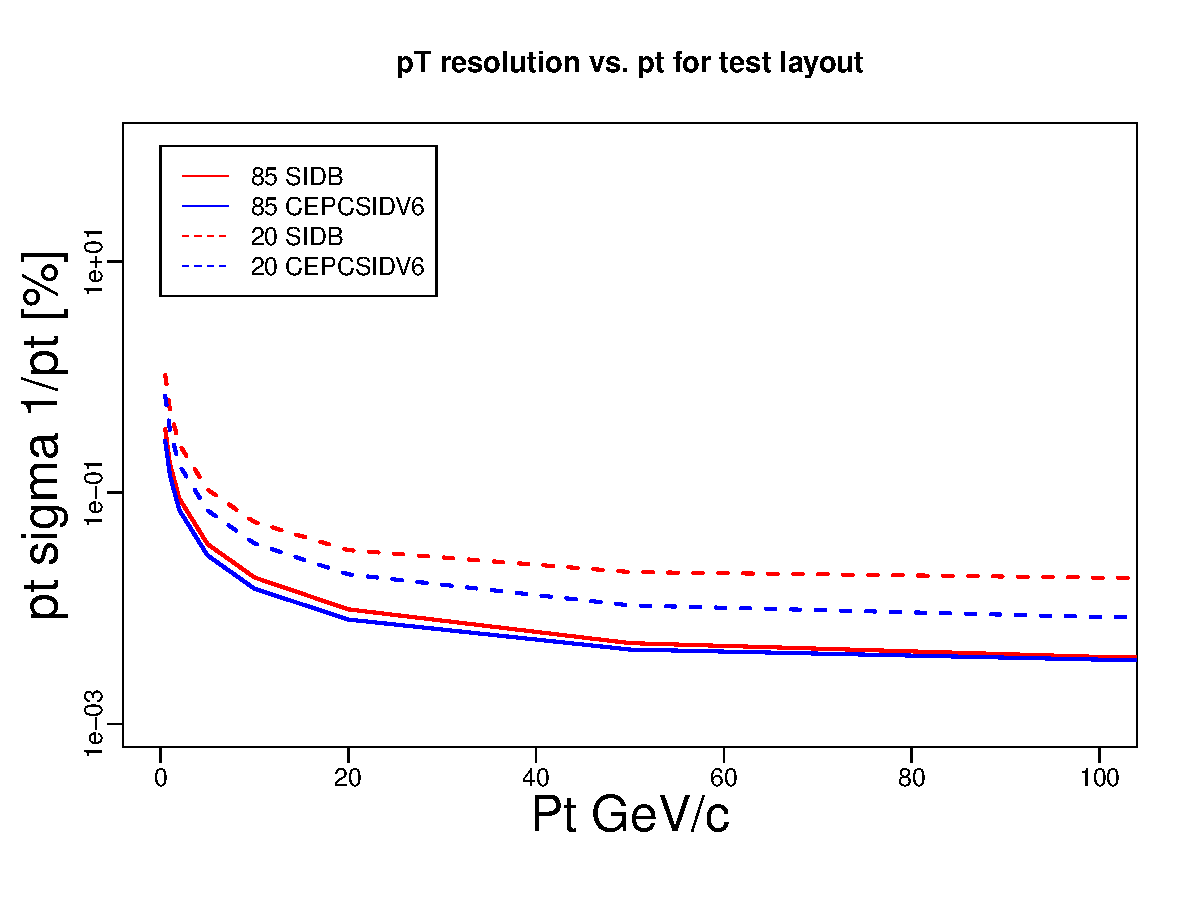
\includegraphics[width=0.32\textheight,keepaspectratio]{Figures/TrackingSystem/FullSilicon/Overlay__ptvsptZ_R.pdf}
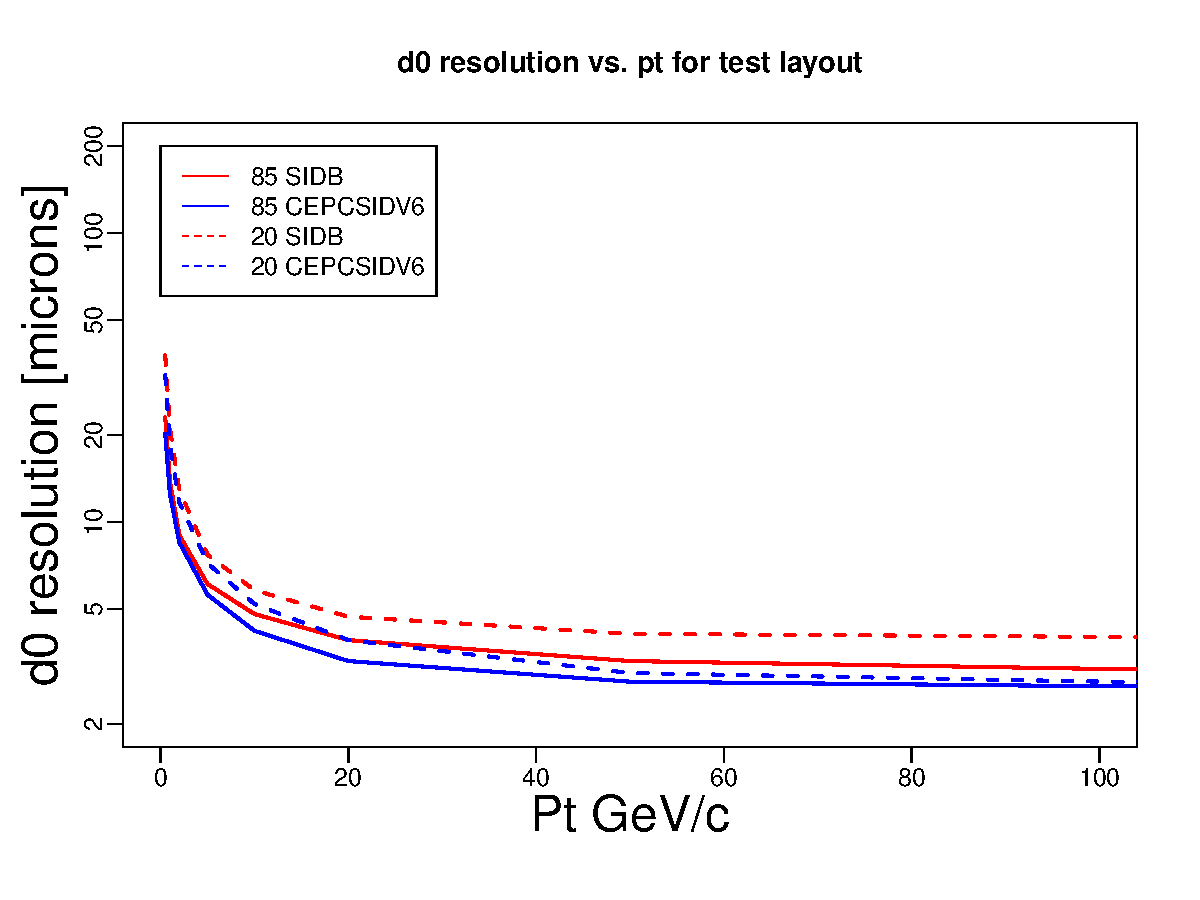
\includegraphics[width=0.32\textheight,keepaspectratio]{Figures/TrackingSystem/FullSilicon/Overlay__d0vsptZ_R.pdf}
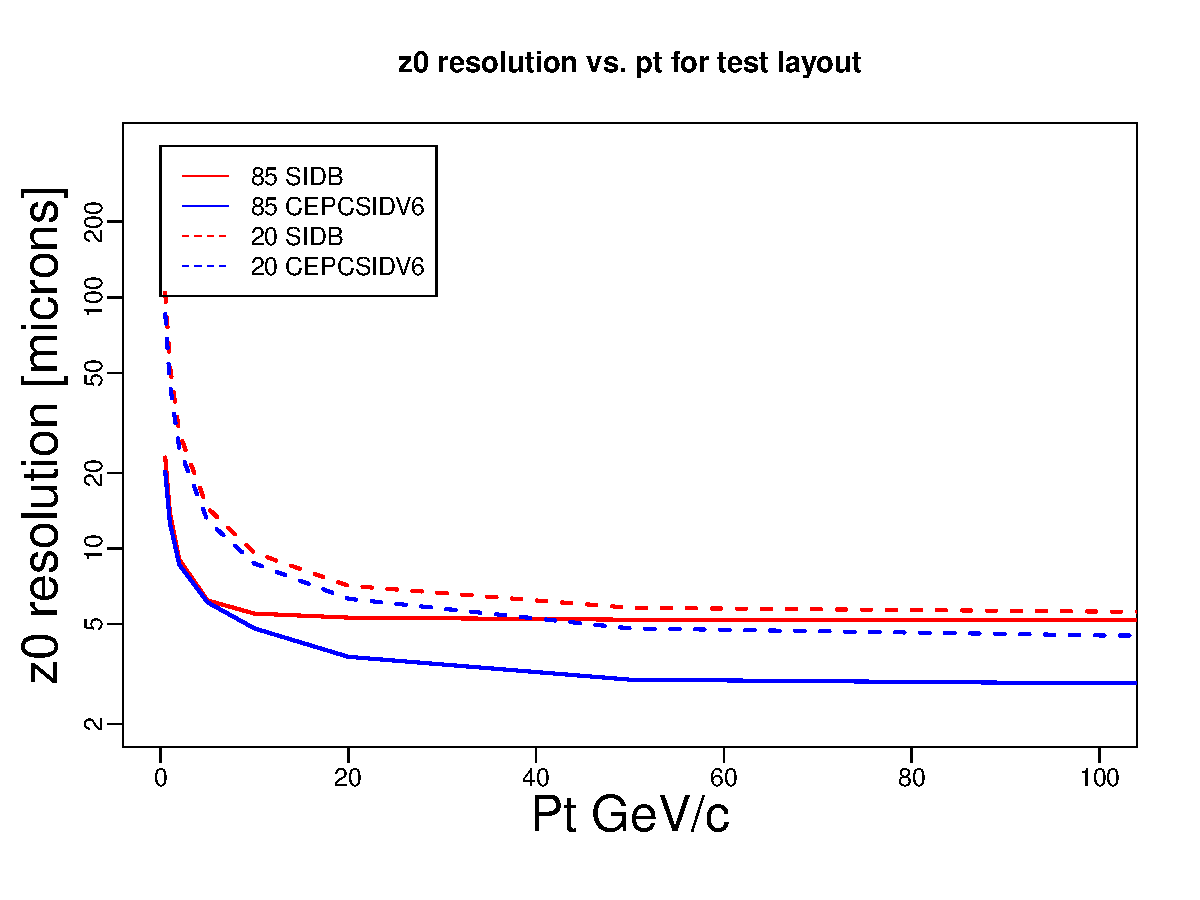
\includegraphics[width=0.32\textheight,keepaspectratio]{Figures/TrackingSystem/FullSilicon/Overlay__z0vsptZ_R.pdf}
\caption{The expected $p_T$, d0, and z0 resolutions from the toy simulation (Idres) are compared as function of track $p_T$ in GeV/c
for tracks with $\theta =$ 85 and 20 degree, respectively. \label{fig:toyptd0z0}}
\end{center}
\end{figure}
   
\subsection{Detector simulation and reconstruction} 
In order to optimize the full silicon tracker detector for CEPC, we generate several benchmark processes that include single muon events, 
$e^+e^- \rightarrow ZH \rightarrow \nu\nu \mu\mu$, and $e^+e^- \rightarrow ZH \rightarrow \nu\nu GG$ (two gluon jets). 
The events are then simulated and reconstructed using 
different detector geometries, which are then used for the tracking performance studies.    

\subsubsection{CEPC-SID detector}
The implement of geometry of full-silicon-tracker is based on a simulation tool Mokka\cite{ilcMokka}. The CEPC group have create a version of 
database cepc\_v4 to build the preliminary design of CEPC detector~\cite{cepcILD}, in which the tracker is composed of VXD, SIT, TPC, SET and FTD. 
In order to implement the full-silicon-tracker, the TPC is considered to be replaced with a new silicon-based strip tracker. Similarly, the new 
silicon tracker is also called as SIT, and the SET is removed at the same time, since the type of the old SIT, the new silicon-based strip tracker 
and the SET are based on the same design. Finally, a full-silicon-tracker including VXD, SIT and FTD is built on the basis of cepc\_v4, as described 
above. 

In order to improve the flexibility of design, a new package of SiTracker is implemented in Mokka which represents the silicon
tracker by planar structure, which consists of a. thin layer of silicon with 150 $\mu m$ thickness and 50 $\mu m$ pitch size. 
For VXD and SIT, they are composed by several layers, and each layer is composed by several ladders, and 
each ladder is divided to several sensors. The SIT layer consist of double silicon layers mounted back to back with a stereo-angle of 7 degree.
For FTD, it is composed by several pixel disks FTD\_PIXEL and several double-side strip 
disks FTD\_STRIP that are composed by petals. The strip FTD disk has two sensitive silicon sub-layers on each side with a stereo-angle of 5 degree.
The number of ladders/petals, the size and position of layers, and the sub-structure of layers can be modified easily in input file as 
globalModelParameter. In future, a XML structure is considered as the method to input parameters.

The lcio format is used to output the simulated signals from the full-silicon-tracker, same as other 
sub-detector system~\cite{lcsim}. The digitization and clustering are done 
in reconstruction process. In the default version, a smearing technology based on truth information 
is used as a simple digitization and clustering, which is used for this study. 
Recently, a new digitization for silicon-based detector has been developed. It first finds out the pixel which the hit is located, and uses the 
center of the pixel or strip as the new position for the hit. And then those hits in same pixel or neighnoring will be merged into single hit.

The silicon tracking algorithm is the same one used by CEPC-ILD~\cite{cepcILD}, which are steered by a set of strategies.
Each strategy represents a set of layers in the detector and tries to find combinations of hits that forms a helix within these layers.
The algorithm starts by looking for a track seed by any combination of three hits that fufils a helix fit. Once found, the track seed is extended
by successively adding more hits that are consistent with the extrapolation of the seed helix.
If fewer than the minimum required number of hits are found, the track candidate is discarded. If the tracks found in different strategies share
more than one hit, only the track with the best fit is kept based on the $\chi^2$ per degree of freedom and the number of hits on the track.
  
\subsubsection{Optimized SID detector}
For the SiD detector optimized for CEPC (or SIDB), events were simulated and reconstructed
using a software developed for the International Linear Collider (ILC)~\cite{Adolphsen:2013kya,Behnke:2013lya}, but
re-worked for the HepSim project \cite{Chekanov:2016sme,Chekanov:2016ppq}.
The response of the SiD detector to physics events
is simulated using the ``Simulator for the Linear Collider'' (SLIC) 5.0  software~\cite{Graf:2006ei}
interfaced with the {\sc Geant4} 10.3p1 program~\cite{Allison2016186}.
The track reconstruction  was performed with the {\sc LCSim} 4.0 package  \cite{lcsim} using
the ``seed tracker'' algorithm as for the SiD detector simulation.
Track candidates with at  least six hits in the silicon pixel and microstrip layers were considered.
Only tracks with a minimum transverse momentum ($p_T$) of $100$~MeV were accepted.
The track-fitting was performed with the following requirements; maximum distance of closest approach (DCA) is $|DCA|<6$~mm, $|z_0|<10$~mm,
and fit $\chi^2 < 10$. The reconstruction includes particle-flow algorithms (PFA)
which enable  identification and reconstruction of individual particles.
The PFA objects can be reconstructed using the software algorithms implemented in
the {\sc pandora} package~\cite{Charles:2009ta,Marshall:2013bda}.

The geometry of SIDB detector is implemented using the compact XML geometry description, which can load and built
at runtime. The main changes over the ILC-SID detector include the reduced B-field from
5~Tesla to 3~Tesla. The outer tracker is scaled up by a factor of about 1.44 to the radius of
1.83~m and $z$ of $\pm$ 2.3~m. The  silicon module sizes were appropriately scaled.
The first inner layer of the barrel vertex detector was positioned at 15~mm, just outside of the beam pipe.
The outer barrel layer of the silicon vertex detector was moved to 100.3~mm (vs 59~mm for the SiD detector), while
other barrel layers are equally spaced. The forward disks, together with the support structures,
were appropriately scaled in $z$ by a factor 1.37.

As for the SiD detector, the barrel tracker consists of five layers of  silicon sensors with 50~$\mu$m  pitch.
The forward tracker has four disks of silicon sensors.
The silicon pixel detector had 20~$\mu$m pitch,  consisting of five layers in the barrel and six disks in the
forward region. The hadronic and  electromagnetic calorimeters, as well as the muon detector,
were optimized for CEPC physics as described in \cite{Chekanov:2016efe}.

\subsection{Tracking performance} 
After the detector simulation and reconstruction, the tracking performances are  measured in terms of efficiencies, 
fake rates, momentum resolution, and the impact parameter resolutions using single muons or $e^+e^- \rightarrow ZH$ events. 
The tracking efficiency is defined as a fraction of stable charged particles that can be matched to well reconstructed tracks. 
The stable particles are defined as those charged particles with $p_T>$1 GeV/c in the detector fiducial region ( $9<\theta<170$ degree), 
originated from the interaction point, and lived long enough to reach the calorimeter. A well reconstructed 
track is defined as sharing more than 50\% of its assigned silicon hits originating from a single particle (truth hits). 
We define a truth hit fraction as ratio of truth hits over total assigned hits of the track using silicon hits only.  A poorly reconstructed track is 
defined to have the truth hit fraction less than 50\%. The fake rate is defined as the fraction of poorly reconstructed tracks out of 
total reconstructed tracks, but this requires a realistic detector simulation, which we are not there yet. 
The tracking performance in the CEPC (v\_4) detector is also shown as the reference.  
    
\subsubsection{Single muon particle} 

Figure~\ref{fig:fullsieff} shows the tracking efficiency for single muons in CEPC-SID  as function of $p_T$. 
The tracking efficiency is close to 100\% at high $p_T$ and slightly lower at small $p_T$. The trend is the same for CEPC v\_4 , which indicate both 
trackers are capable of finding tracks efficiently in the detector fiducial region. 

\begin{figure}[hbtp]
\begin{center}
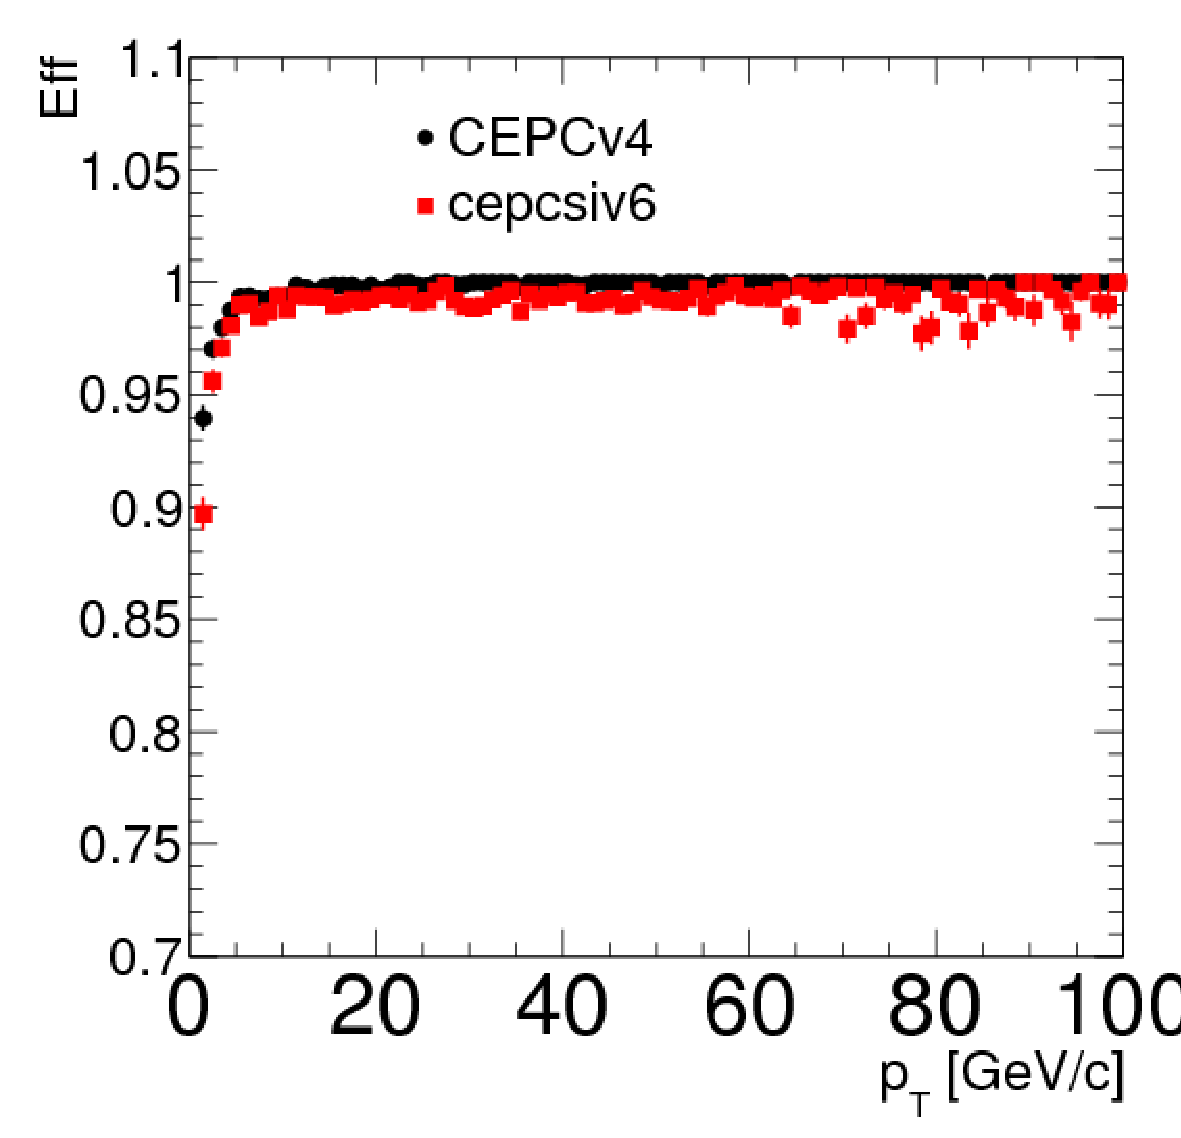
\includegraphics[width=0.45\textheight,keepaspectratio]{Figures/TrackingSystem/FullSilicon/Plot_muon_Eff_Pt.pdf}
\caption{The tracking efficiencies are measured as function of $p_T$ for single muons using CEPC v\_4 and 
CEPC-SID detetcors. \label{fig:fullsieff}}
\end{center}
\end{figure}

The number of silicon hits found on the track and the fraction of truth hits  are shown in Fig.~\ref{fig:fullsinhit} where the hit 
purity is reached more than 90\% for both detectors. 

\begin{figure}[hbtp]
\begin{center}
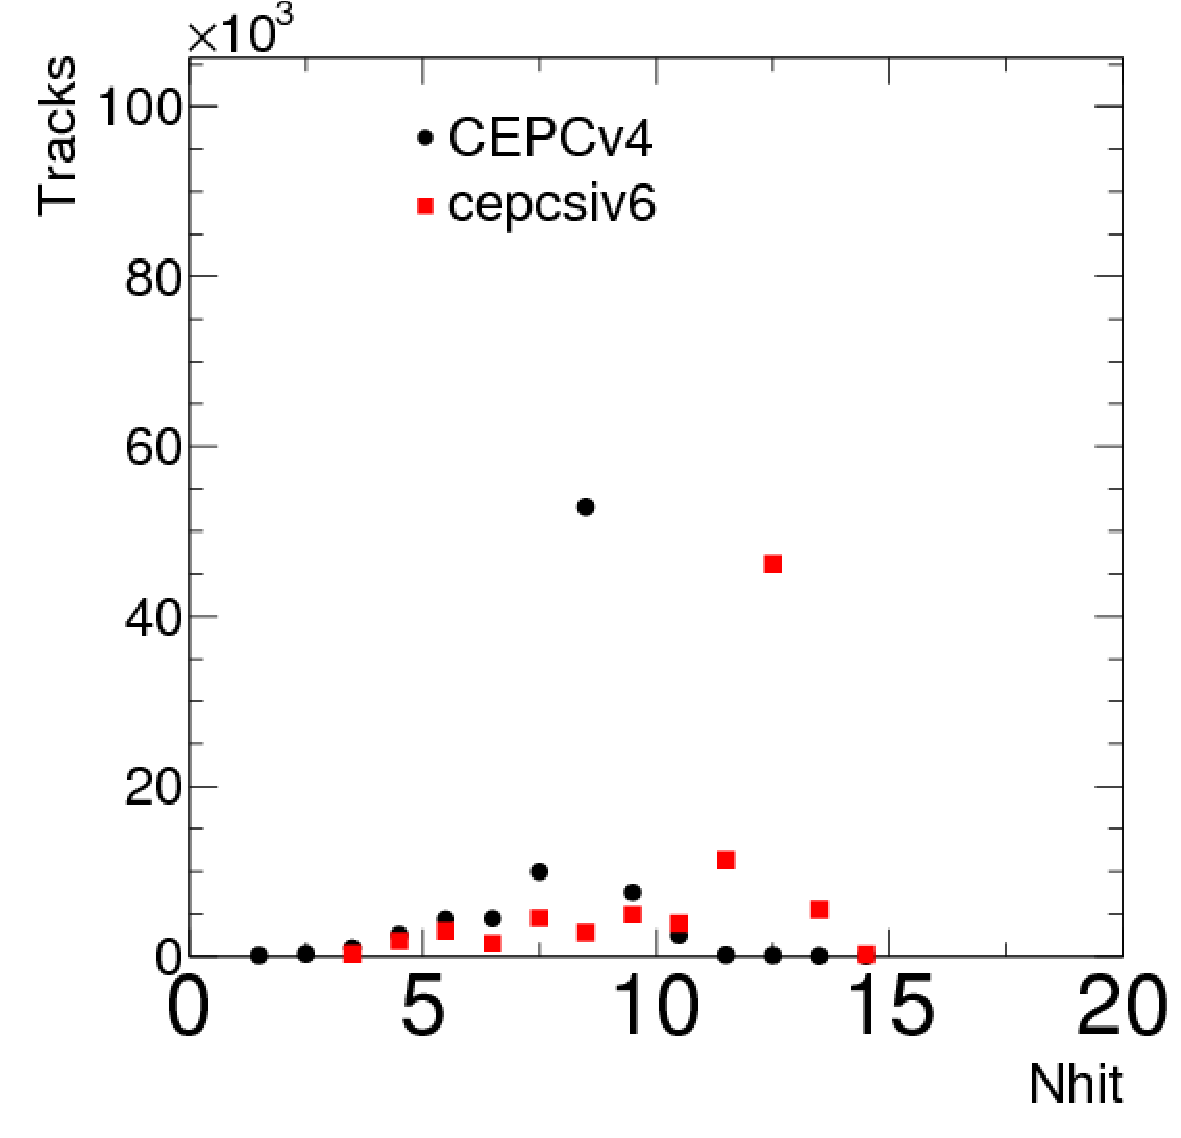
\includegraphics[width=0.45\textheight,keepaspectratio]{Figures/TrackingSystem/FullSilicon/Plot_muon_Nhit.pdf}
\caption{The distributions are shown for the number of silicon hits on the track (left) and the hit purity on (right).\label{fig:fullsinhit}}
\end{center}
\end{figure}


Since the track resolution depends on the track angle $\theta$, we divide the tracks in the barrel 
region with $40<\theta<140$ degree and in the endcap region with $7.25<\theta<40$ degree or $140<\theta<172.75$ degree. 
Figure~\ref{fig:detptd0z0} shows the track resolutions of $p_T$, d0, and z0 as function of track $p_T$ in the barrel and endcap region. 
The resolutions for the low momentum tracks seem slightly better in the CEPC v\_4 detector (TPC+Silicon) than an alternative full silicon tracker due 
to extra materia in the detector while they are compatible at the high $p_T$. 
The resolutions from the SIDB detector are also included in the comparision, which has a compatible momentum resolution 
while the d0 and z0 are slightly worse.

\begin{figure}[hbtp]
\begin{center}
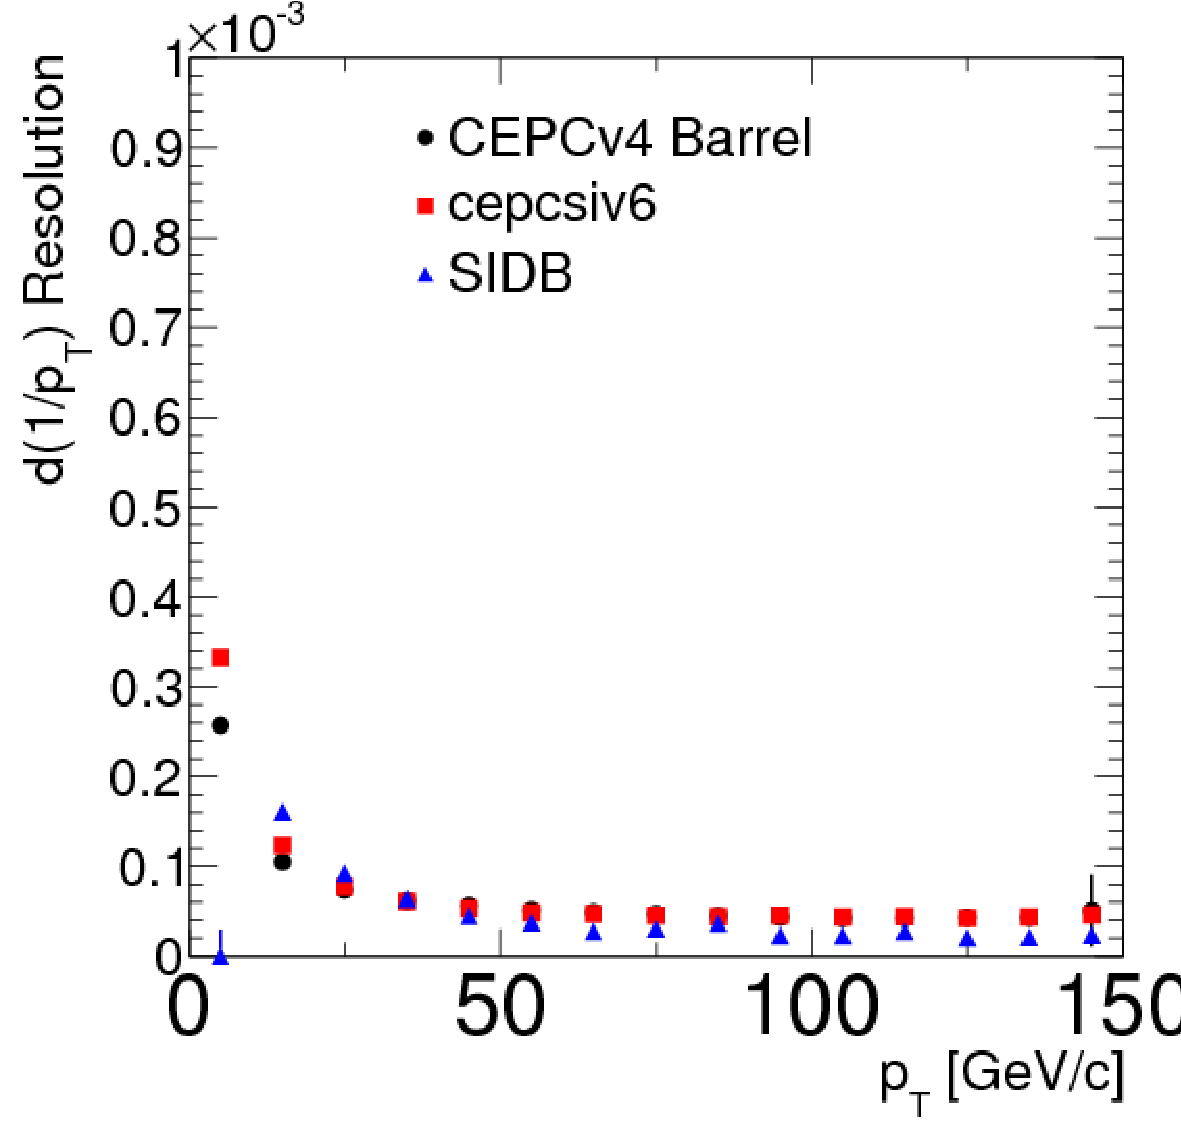
\includegraphics[width=0.25\textheight,keepaspectratio]{Figures/TrackingSystem/FullSilicon/Plot_muon_Pt_PtBarrel.pdf}
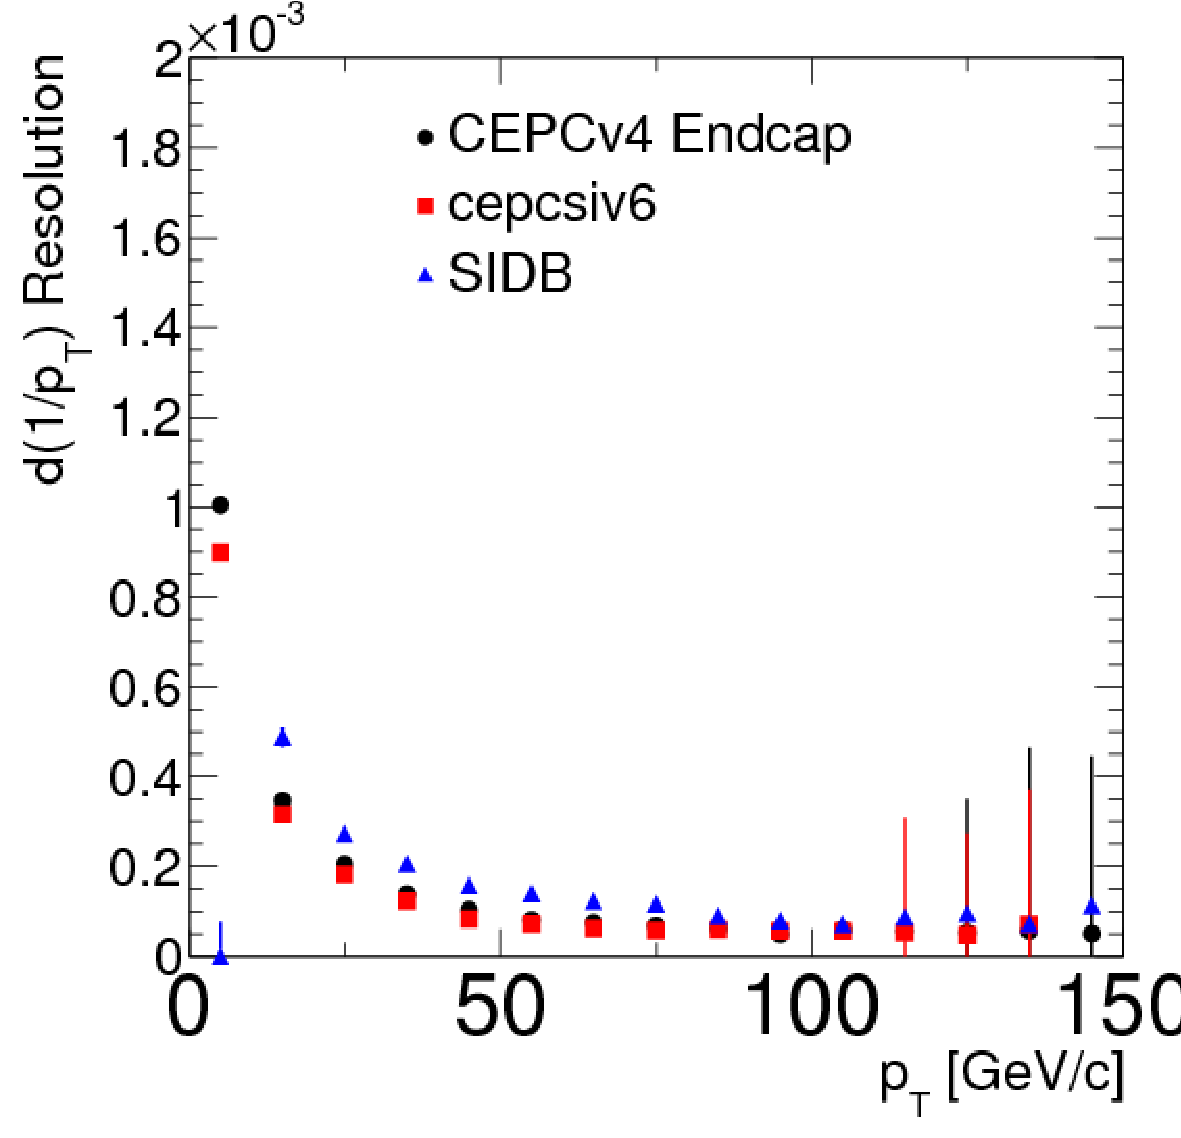
\includegraphics[width=0.25\textheight,keepaspectratio]{Figures/TrackingSystem/FullSilicon/Plot_muon_Pt_PtEndcap.pdf}
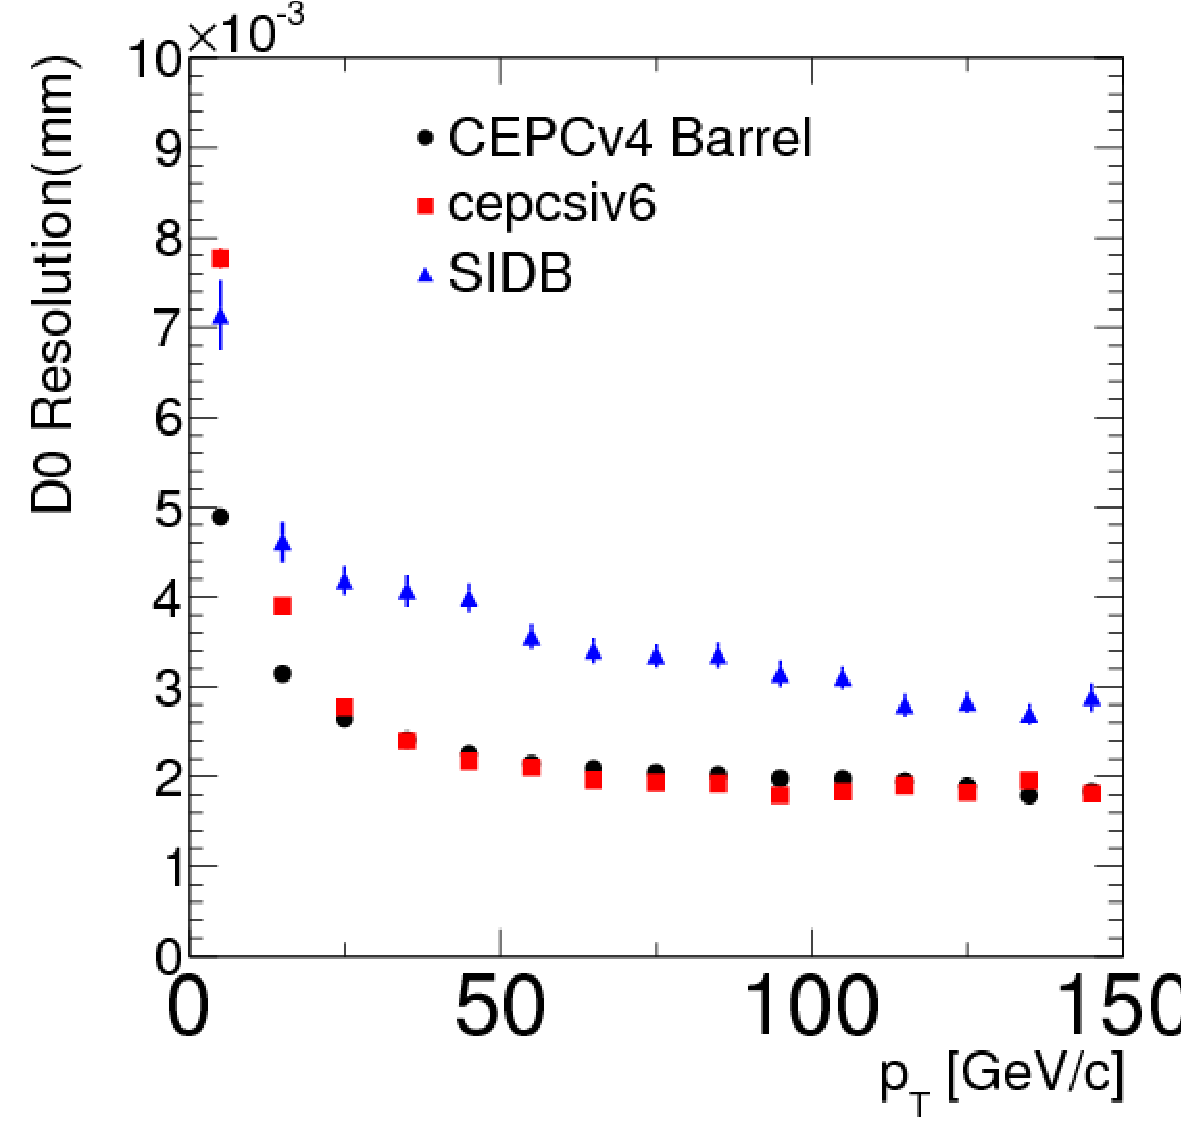
\includegraphics[width=0.25\textheight,keepaspectratio]{Figures/TrackingSystem/FullSilicon/Plot_muon_D0_PtBarrel.pdf}
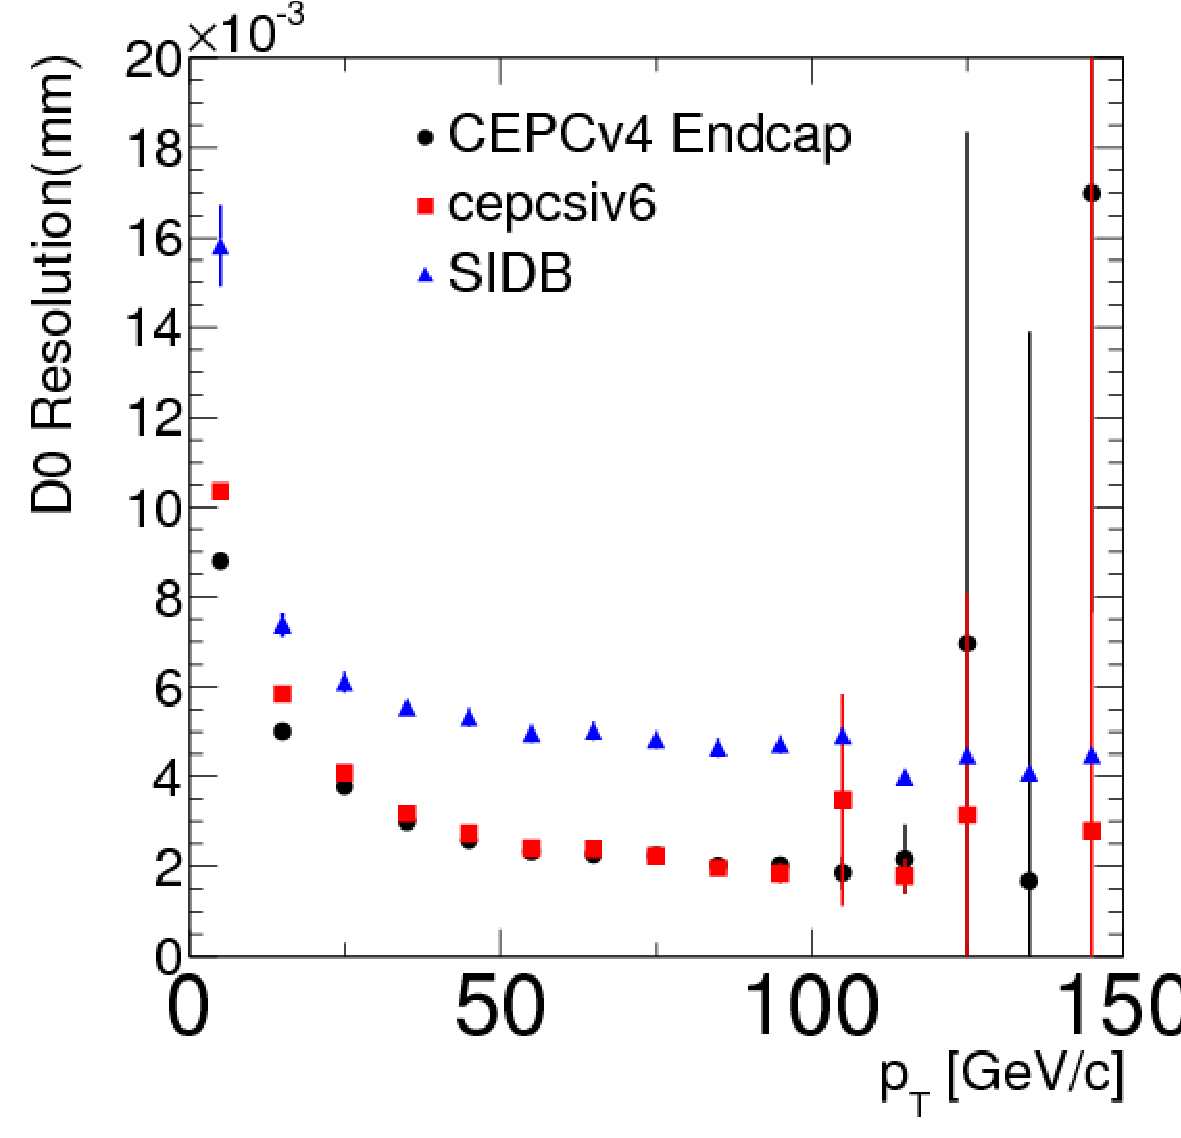
\includegraphics[width=0.25\textheight,keepaspectratio]{Figures/TrackingSystem/FullSilicon/Plot_muon_D0_PtEndcap.pdf}
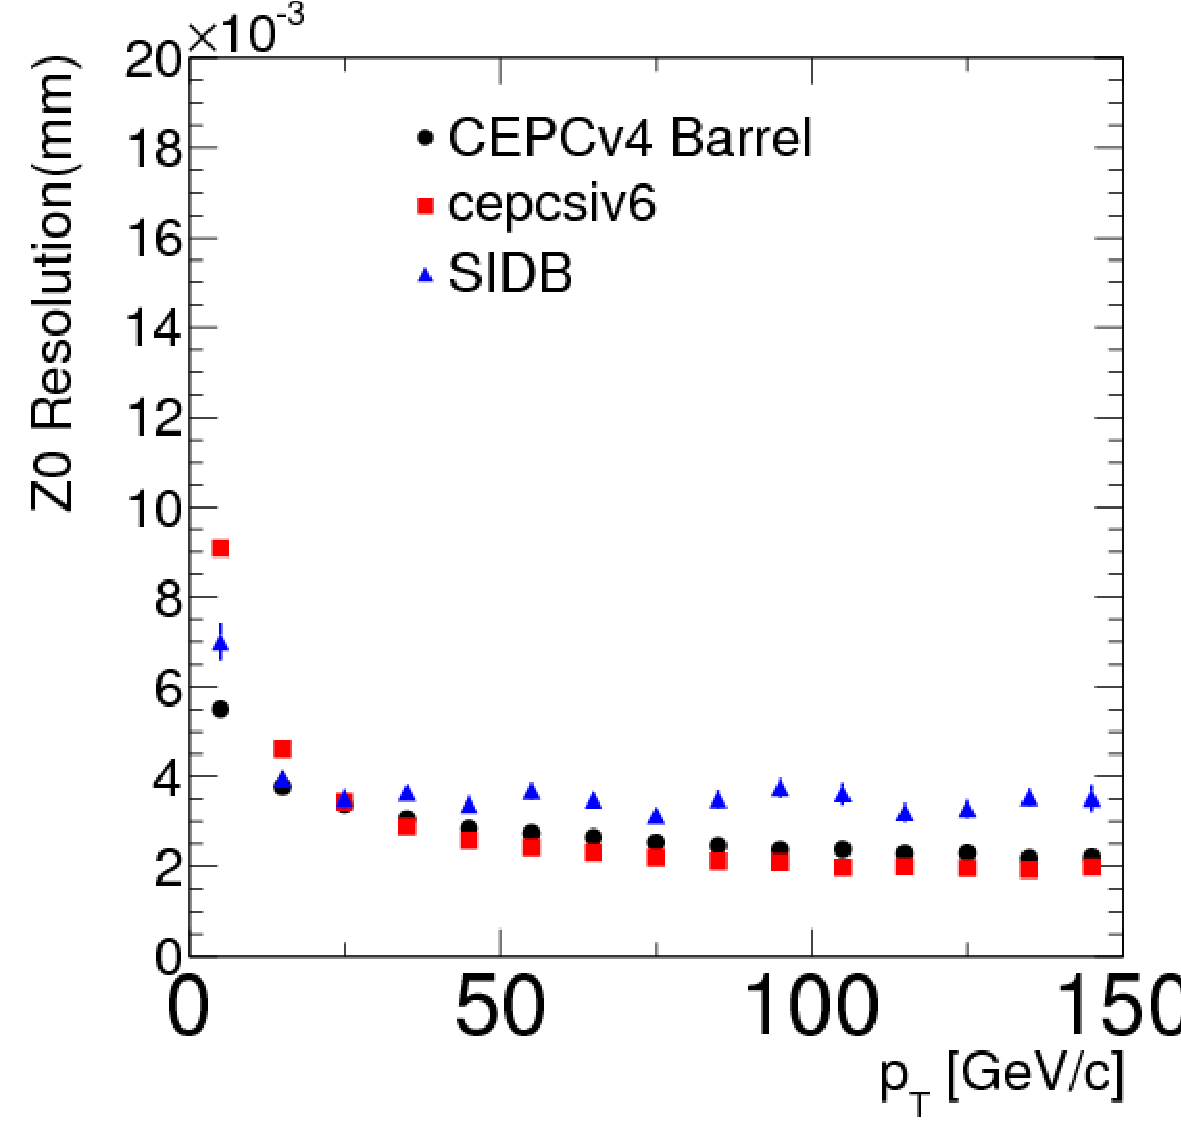
\includegraphics[width=0.25\textheight,keepaspectratio]{Figures/TrackingSystem/FullSilicon/Plot_muon_Z0_PtBarrel.pdf}
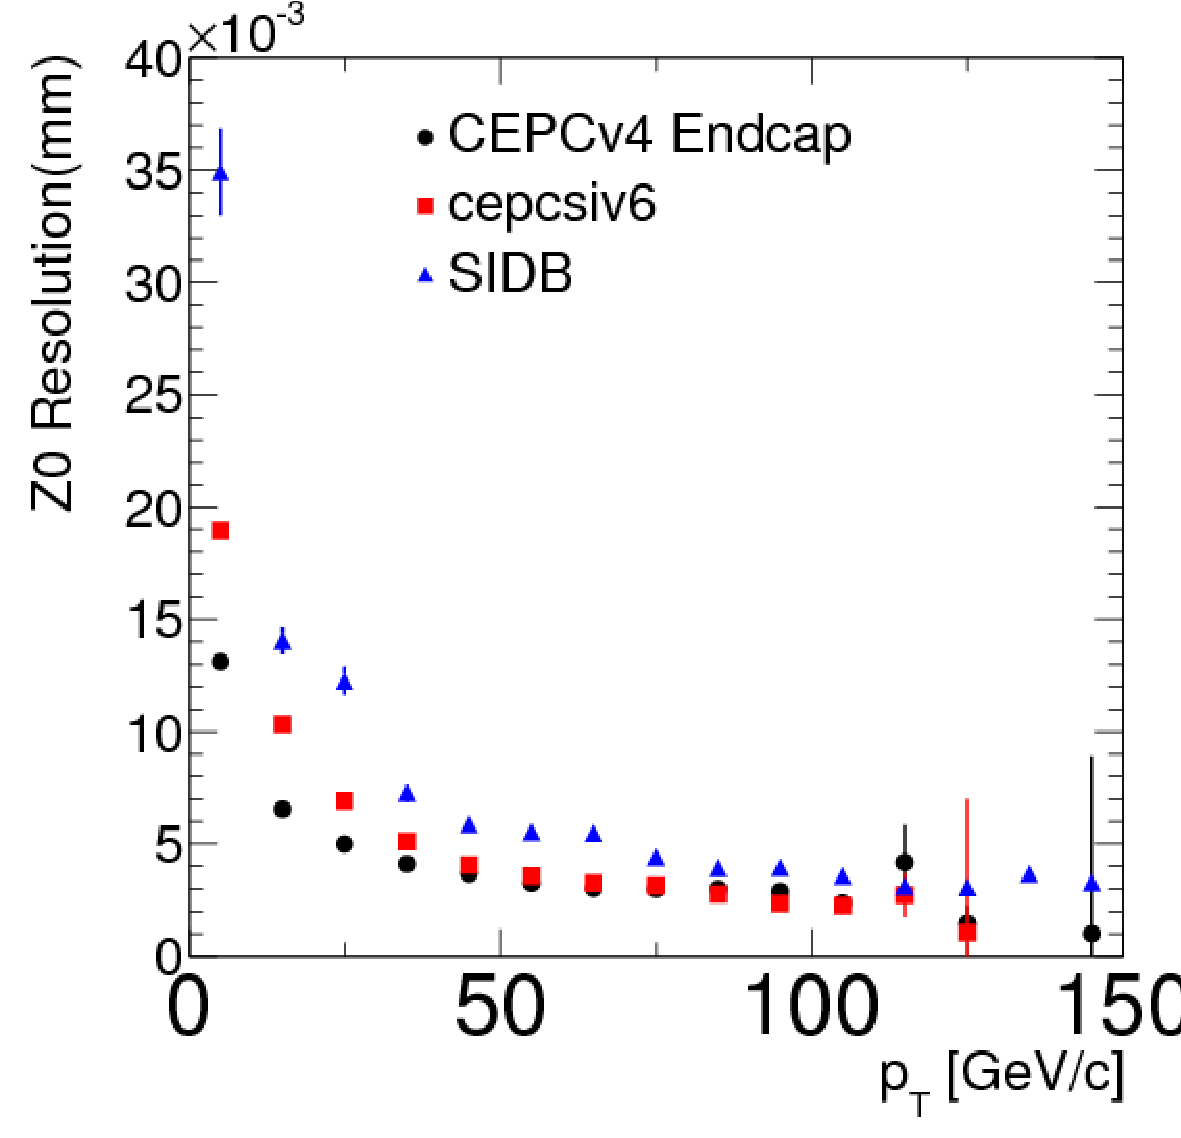
\includegraphics[width=0.25\textheight,keepaspectratio]{Figures/TrackingSystem/FullSilicon/Plot_muon_Z0_PtEndcap.pdf}
\caption{The tracking $p_T$, d0, and z0 resolutions are measured as function of $p_T$, $\phi$, and $\theta$ using single muons, 
left in the barrel region and right in the endcap region. They are compared between CEPC v\_4 and two full silicon detector concepts.\label{fig:detptd0z0}}
\end{center}
\end{figure}
 
\subsubsection{Di-muon mass resolution} 

Figure~\ref{fig:dimuons} shows the di-muon invariant mass distributions from $ZH\rightarrow \nu\nu \mu\mu$ decay between
different detector configurations. The higgs mass used in CEPC simulation is 125 GeV/c$^2$ while 125.09 GeV is used in the SIDB simulation. 
The di-mass from CEPC-ILD seems shifted by 0.2 GeV from the input Higgs mass of 125 GeV/c$^2$ while other masses from CEPC-SID and SIDB
agree with the expectation. The di-muon mass resolution from CEPC-SID has $\sigma=0.21$ GeV/c$^2$ and seems 20\% and 25\% better 
than ones obtained from CEPC-ILD and SIDB, respectively. 

\begin{figure}[hbtp]
\begin{center}
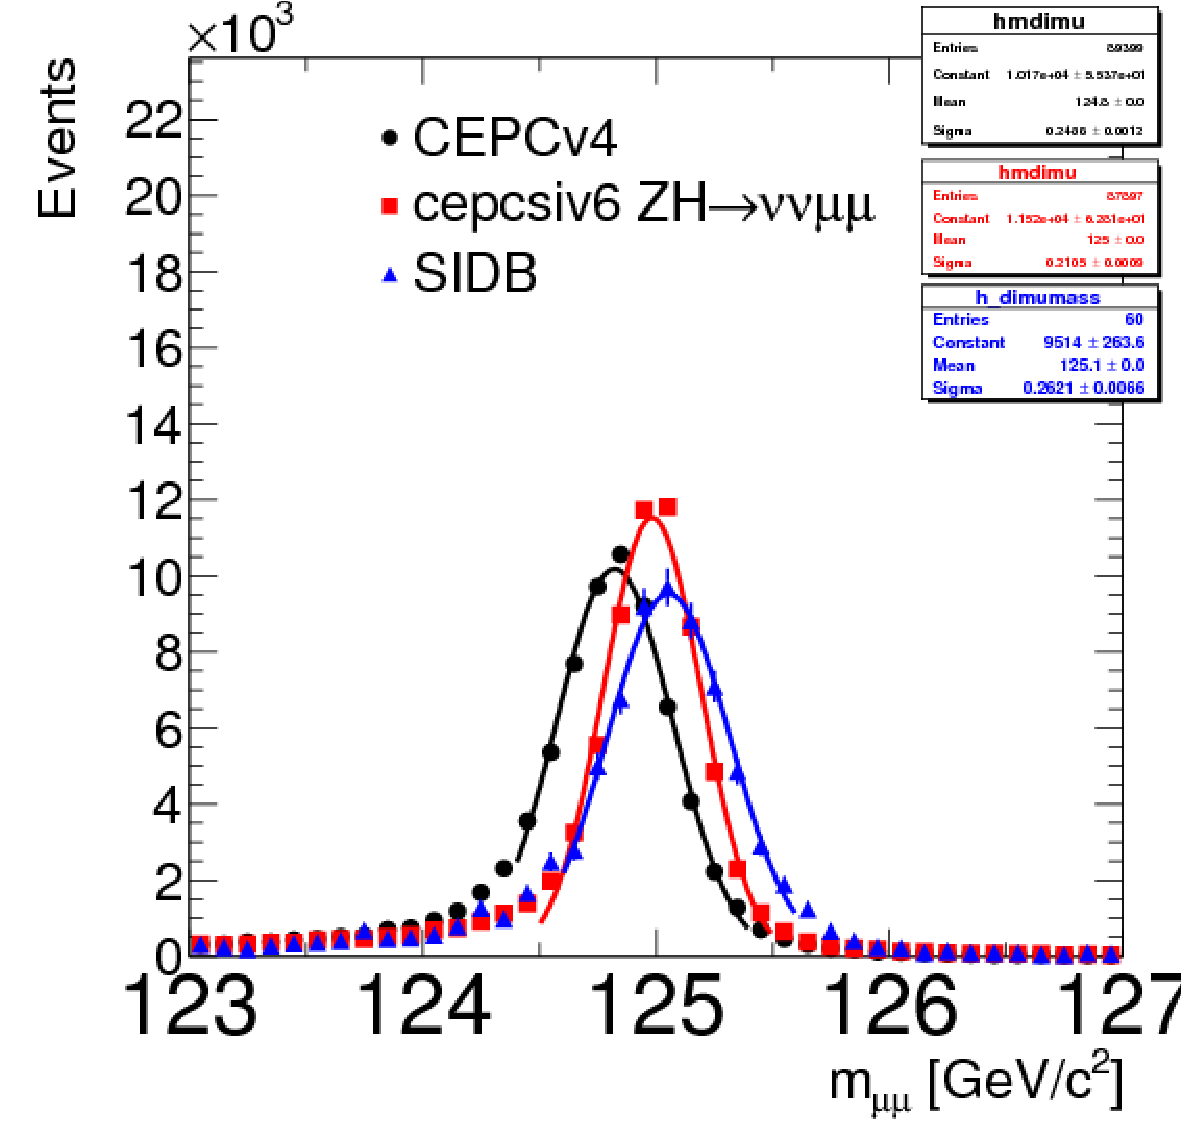
\includegraphics[width=0.45\textheight,keepaspectratio]{Figures/TrackingSystem/FullSilicon/Plot_zhnnmumu_DimuonMass.pdf}
\caption{The di-muon mass distribution is compared from different detectors.\label{fig:dimuons}}
\end{center}
\end{figure}

\subsubsection{Tracking inside the jets} 

In order to study the tracking performance inside the jets, we generated and simulated some Higgs decaying into two gluon jets (GG) in 
$zH\rightarrow \nu\nu GG$ events. Figure~\ref{fig:glgl} shows the tracking efficiency inside the jets as function of track momentum.
The average efficiency of finding tracks inside the jets is about 90\% for CEPC-SID while about 97\% for 
CEPC-ILD due to the excellent tracking in TPC. The full silicon tracking inside the dense of jets is not fully optimized in 
dealing with outliers in the fit, which requires a realistic detector simulation and clustering. The work is in progress to improve
the tracking inside the jets.  
 
\begin{figure}[hbtp]
\begin{center}
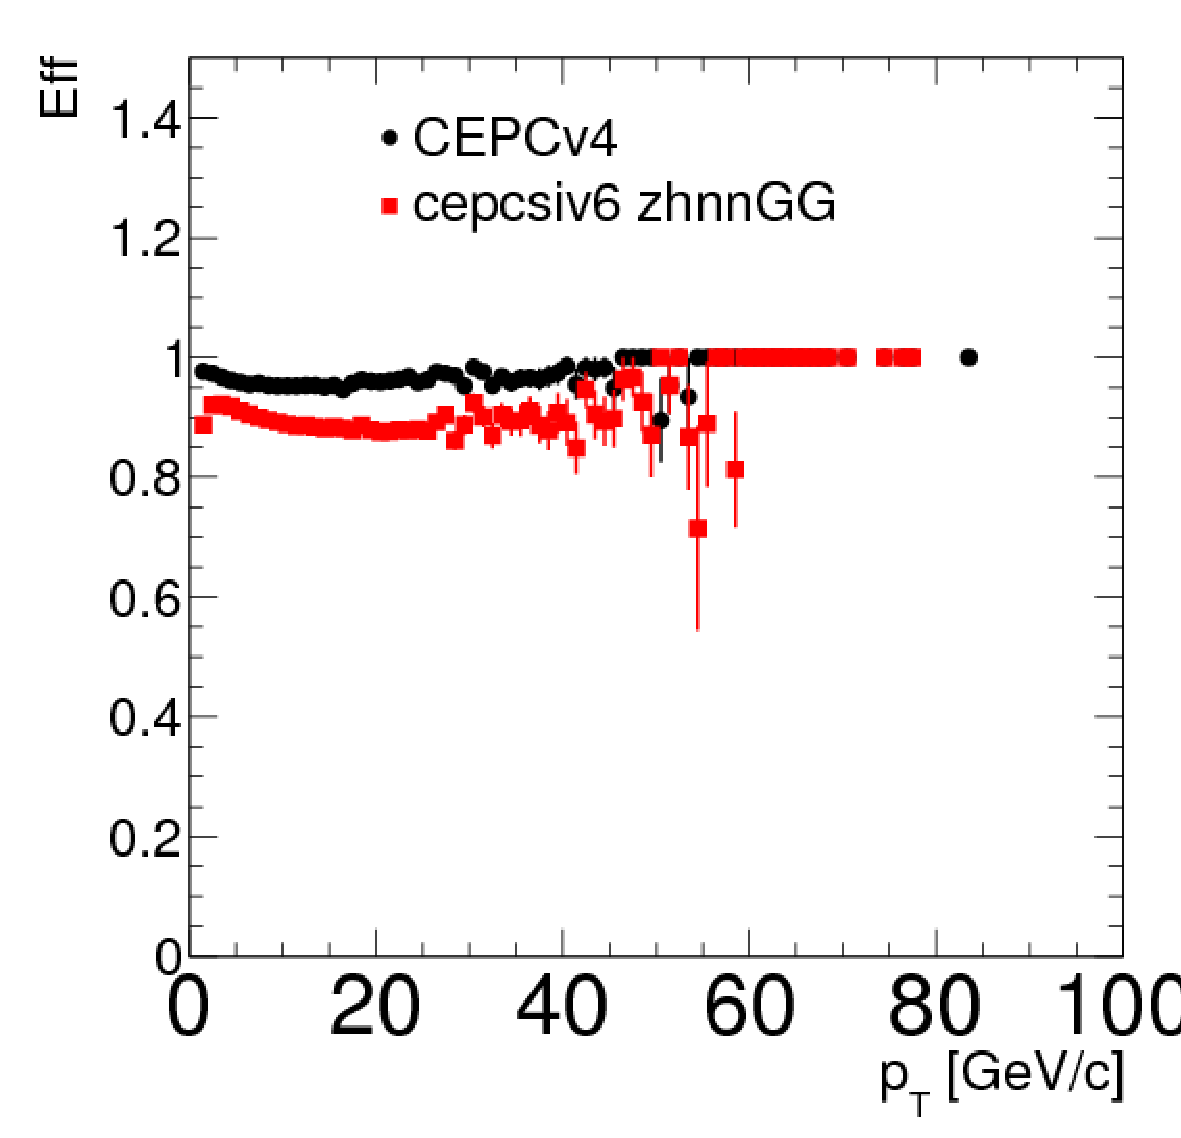
\includegraphics[width=0.45\textheight,keepaspectratio]{Figures/TrackingSystem/FullSilicon/Plot_zhnnGG_Eff_Pt.pdf}
\caption{The tracking efficiencies for the stable particles inside the gluon jets as 
function of track $p_T$ with CEPC v\_4 and CEPCSID.\label{fig:glgl}}
\end{center}
\end{figure}

\subsection{Conclusion} 
  We present a preliminary study of full silicon tracker option as an alternative design for CEPC tracking.
  Two approaches are considered for the design: the first is to keep the
  silicon detectors (VXD, SIT, FTD) in the CEPC-ILD detector and replacing TPC with additional silicon detectors,
  the second is to optimize the ILC-SID tracker to fulfil the CEPC tracking volume in order to achive the
  excellent momentum resolution using 3 Tesla B field. The new detector geometry has been implemented in
  the simulation and the track reconstruction has also been adoped for the full silicon tracker.
  The initial study of the tracking performance looks promising. There are still many improvements 
  needed in the simulation and reconstruction in order to explore the full potential of the full-silicon tracker. 



\section{Drift chamber tracker detector}


%\begin{figure}[h!]
%\centering
%\includegraphics[scale=0.32] {Figures/TrackingSystem/7p_L_HL_CC.pdf}
%\includegraphics[scale=0.80] {Figures/TrackingSystem/fig_HCfit10.pdf}
%\caption{Top: The 7 parameter fit, and comparison with the HL-LHC, discussed in detail in %Chapter~\ref{Chapter:Higgs}. The projections for CEPC at 250 GeV with 5~ab$^{-1}$ integrated %luminosity are shown. The CEPC results without combination with HL-LHC input are  shown with dashed edges. The LHC projections for an integrated luminosity of 300 fb$^{-1}$ are shown in dashed edges. Bottom: Comparison between the LHC and several benchmark luminosities of the CEPC. }
%\label{fig:7param}
%\end{figure}


\bibliographystyle{Style/atlasnote} %% plain.bst
\bibliography{Chapters/TrackingSystem} %% bsample.bib


\chapter{Calorimetry}
\label{Chapter:Calorimetry}

\section{Introduction to calorimeters}
\label{sec:intro}
%
Calorimeters of the CEPC detector, including electromagnetic calorimeter (ECAL) and hadron calorimeter (HCAL), are employed for precise energy measurements of electron, photon, tau and hadronic jets. To fully exploit the physics potential about Higgs, W, Z and related SM processes, the jet energy resolution $\sigma_{E}/E$ is required to reach 3\%-4\%, or $30\%/\sqrt{E}$ at energies below about 100~GeV. This resolution is about a factor of two smaller than the calorimeters used for the LEP detectors and currently operating calorimeters at the LHC. It significantly improves the separation of the W and Z bosons which decay into two jets, as shown in Figure~\ref{fig:cal-WZ}. The basic requirements for ECAL and HCAL resolution are $16\%/\sqrt{E}$ and $50\%/\sqrt{E}$, respectively.\\
%
\begin{figure}[tbp]
\centering
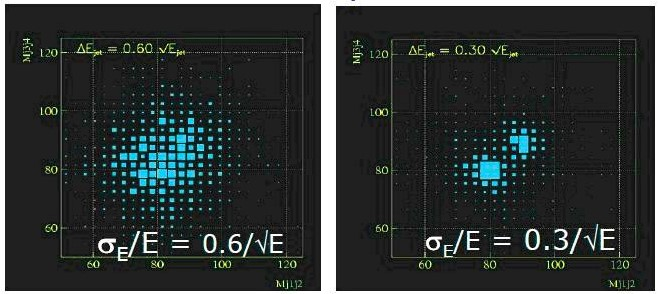
\includegraphics[width=14.cm]{Figures/Calorimetry/cal-WZ-separation.jpg}
\caption{\label{fig:cal-WZ} Separation of W and Z bosons with different jet energy resolutions.}
\end{figure}
%

To achieve the required jet energy resolution, many R\&D researches are carried out within the CALICE collaboration since 2000~\cite{calice}. The majority of these studies aim to develop extremely fine granularity and compact imaging calorimeters with several technology options shown in Figure~\ref{fig:cal-PFA}. Imaging calorimeter is a rapidly developing novel particle detector which has excellent spatial resolution. It is capable to provide enormous position information of incident and showering particles, which makes it possible to reconstruct every single particle cluster. This is vital for Particle Flow Algorithm (PFA~\cite{cha411}) and help to significantly improve the energy resolution of hadrons. The basic idea of PFA is to distinguish charged ($\sim$65\%) and neutral particles ($\sim$35\%) inside the calorimeters. Charged particles measured in the inner tracker with high momentum resolution are matched to their energy depositions in the calorimeters. Energy depositions without matched inner tracks are considered to originate from neutral particles inside jets, among these neutral particles, about 25\% of energy from photons are measured in the ECAL with good energy resolution, while the residual energy of merely 10\% from neutral hadrons are measured by the calorimeters with poor energy resolution. Hence, the jet energy is determined by the charged track momenta of charged particles from inner tracker and energy depositions of neutral particles in the calorimeters. It has been demonstrated that significant improvement of the jet energy resolution is achievable based on MC simulations and test beam measurements. However, more efforts are needed to optimize the calorimeter design, to improve the PFA, and
to develop the technologies for high granularity imaging calorimeters.\\

%
\begin{figure}[tbp]
\centering
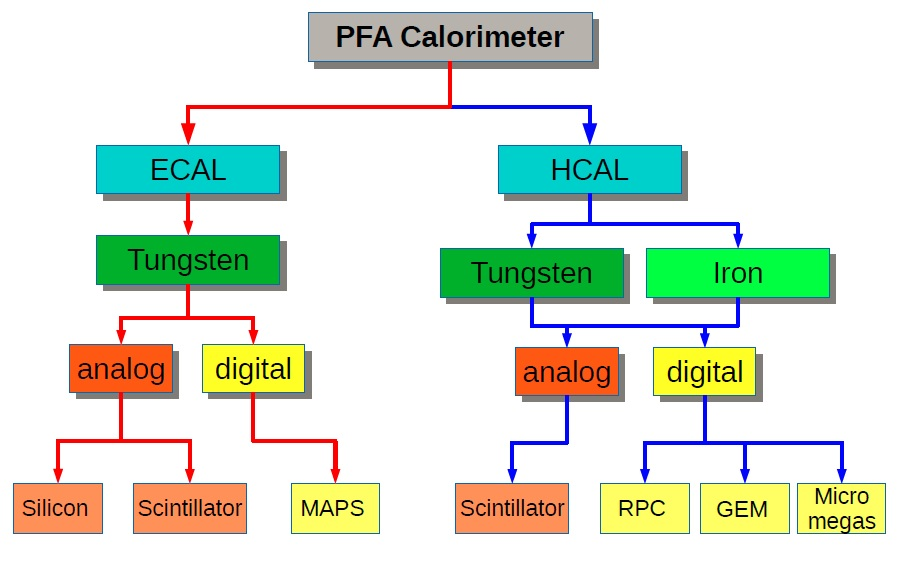
\includegraphics[width=14.cm]{Figures/Calorimetry/cal-PFA.jpg}
\caption{\label{fig:cal-PFA} PFA: Imaging calorimeters being developed by the CALICE collaboration since 2000.}
\end{figure}
%

The calorimeter system includes two sub-detectors, an electromagnetic calorimeter (ECAL) which is optimized for the
measurement of photons and electrons, and a hadronic calorimeter (HCAL) which is employed to measure the energy
deposit of the hadronic showers caused by the hadronic particles when they are absorbed in the HCAL detector. The
two sub-detectors will be installed within the solenoid to minimize the inactive material in front of the calorimeters
and to reliably associate tracks to energy deposits. The calorimeter system is divided into three parts, one cylindrical
barrel and two end-caps.

The ECAL consists of layers of active sensors (such as silicon pads or pixels, or scintillator detector) interleaved
with absorber tungsten plates. The digital HCAL (DHCAL) is expected to have stainless steel absorber plates with gaseous detectors
such as glass Resistive Plate Chambers (gRPC) or GEM, or analog HCAL (AHCAL) using scintillator with SiPM readout as sensor.
Both ECAL and HCAL are sampling detectors with very fine granularity and segmentations of electronic readout
which is driven by excellent separations requirement between charged and neutral particles for the particle flow algorithms.

From Figure~\ref{fig:cal-PFA}, there are more detector options with enormous worldwide R\&D efforts ongoing within the
CALICE collaboration.
Another approach for high performance calorimeters is dual-readout calorimetry.

However, for this particular CDR, we have to be selective and focus on a few options with collaborators
who expressed great interests so far. The CEPC detectors R\&D is widely open for international
collaboration with different detector options and new ideas.

%%%%\\\\\\\\\\\\\\
\section{Electromagnetic Calorimeter for Particle Flow Approach}
%
The particle flow paradigm has tremendous impact on the design of the electromagnetic calorimeter detector. Separating overlap showers from each other is principal requirement of the detector. A calorimeter used for particle flow thus needs to be able to do pattern recognition in the shower. The electromagnetic section has lots of tasks to fulfill. It should be able to select photons from close-by particles. It should be able to reconstruct the detailed properties of the shower, such as shower shape, starting point and energy distribution. It should be able to distinguish early starting electromagnetic showers from hadronic ones. The imaging capabilities of the calorimeter are more important than the intrinsic single particle energy resolution, although the latter is still important to the particle flow performance for electron, photons and jets. Due to the reason that about half of the hadronic showers will start development inside the electromagnetic calorimeter, a calorimeter with excellent three dimensional granularity is of utmost importance. In order to have the ability of separate close-by showers in the calorimeter, the detector with small Moliere radius is required. A large ratio between interaction length and radiation length of the detector is advantageous to the separation between electromagnetic and hadronic showers. A small radiation length will make the start of the electromagnetic shower earlier in the calorimeter, while a large interaction length will reduce the fraction of hadronic showers starting in the calorimeter. At the same time, the calorimeter with a compact structure is favorable.\\

In this section, we focus on two detector options for the ECAL, which consist of layers of active sensors (silicon pads or pixels, or scintillator detector) interleaved with absorber tungsten plates.


\subsection{Silicon-Tungsten Sandwich Electromagnetic Calorimeter}
\subsubsection{Introduction}

The study of the Higgs is not the only goal of a machine at 250 centre-of-mass
energy. It can be generalised to the multi boson physics (Z, W and H). The best
way to use the excellent luminosity foreseen at CEPC, consist to tag the boson
through their mass in their decays into $q\bar{q}$ (2 jets). Taking into account
the natural width of the Z and W, it has been shown that this goal required to
achieve a jet energy resolution of $30\%/\sqrt{E_\mathrm{Jet}}$, thus a factor
two better than the energy resolution achieved for a typical detector at LEP.

It has been shown~\cite{Videau:2002sk} that a method consisting to fully
reconstruct every single particle could reach this goal (Particle Flow
Algorithm); it requires both a high performance tracker, typically achieving
$\delta p / p$ of $10^{_5} p / GeV$ associated with high granularity
calorimeters able to separate the contribution from individual particles down to
the MIP level. %
As a typical jet is contains fractions in energy of 65\%, 25\% and 10\% of
charged particles, photons and neutral hadrons respectively, a moderate
calorimetric resolution is then sufficient to achieve the goal. %
In this framework, the electromagnetic calorimeter (ECal), is first devoted to
measure photon(s) and to a lesser extent electron(s) and to make a full pattern
of the deposited energy of the hadron, i.e. shower of hadron interacting in the
ECAL. %
To avoid ``blind region'', the entire calorimeter has to be put inside the
super-conductive solenoid. The compactness is therefore an important criterion.

The design of the calorimeters have to take the following guidelines into
account~\cite{Videau:2002qf}:
\begin{itemize}
\item Optimisation of the number of calorimeter cells (cell size and number of
  layers)
\item Choice of the absorber material in order to insure a high level of
  compactness and the infra-structural components such as cooling, power
  supplies, readout cables and the very front end electronics.
\end{itemize}
For the electromagnetic calorimeter these criteria has led to the choice of
Tungsten with a radiation length of Xo=3.5{mm}, a Moli�re radius of
RM=9{mm} and an interaction length of $\lambda_\mathrm{I}=96{mm}$.

\subsubsection{Silicon sensors}
\label{sec:SiW-Si}

Among several sensor techniques, high resistivity silicon pin diodes offer
several unique intrinsic advantages:
\begin{itemize}
\item stability: under a reasonable bias voltage, completely depleted pin-diode
  have a gain of one, and a signal response to MIP mostly defined by the
  thickness of the sensor, with a very low dependence on temperature, radiation,
  humidity, ...
\item uniformity: for the same reason, the control of the thickness over large
  batches (typically to less than a percent) ensures a uniformity of response
  within a wafer and between them. %
  The nonsensitive area between wafers has recently been reduced by the use of
  laser cutting, thinned guard-ring design~\cite{Cornat:2009zz}, and would
  benefit from the use of larger ingot size (8'' becoming the standard).
\item flexibility: the dimension and geometry of the cells are defined by the
  readout pad on the PCB.
\item High Signal-to-Noise ratio: with $\simeq80$ electron-hole pairs created by
  linear mm of MIP track, MIPs tracks can easily be traced in the calorimeters,
  which is critical for the god performance of
\end{itemize}
The only real drawback of Silicon sensors remaining is their price, to be
expected around $2-3{\$/cm^2}$.

By associating of Silicon sensors with Tungsten absorbers and Carbon Fibre
structures, the SiW-ECAL offers an excellent option for PFA optimised
calorimetry.

\subsubsection{Constraints}
\label{sec:SiW-Constraints}

High granularity calorimetry, and ECal especially, is technically challenging:
the very number of channels calls for an embedded readout and zero suppression,
to limits the amount of connections; in turn embedded readout power consumption
should be as limited as possible to avoid large cooling systems which would
degrade the capacity of the calorimeter. In the best case the cooling should
stay passive at the heart of the calorimeters.

The design proposed for the CEPC SiW-ECal is very largely inspired by the one of
the ILD detector for ILC as described in the Detector baseline
Document~\cite{ILD_DBD:2013}; it is influenced by the options studied for the
CMS High-Luminosity upgrade endcap replacement HGCAL~\cite{Magnan:2017exp,
  Martelli:2017qbe}, concerning cooling and electronics. In terms of luminosity
and collision rates, the CEPC lies between the 2 options.

\subsubsection{Mechanics \& design}
\label{sec:SiW-Design}

The geometry presented here reflects the current (october 2017) status on the
realistic models developed for ILD. It differs slightly form the CEPC\_v1 and
CEPC\_v4 models~\cite{Zhao:2017}, mainly on ECAL thickness ($223{mm}$ vs
$185{mm}$), and inner radius of the endcaps ($226.8$ and $245{mm}$ vs
$400{mm}$).

% CEPCv1
% Barrel R = 1843-2028 mm (thickness = 185mm)
% Endcaps Z = 2450-2635mm (thickness = 185mm) ==> L = 4900mm
% Endcaps Rin = 226.8mm
% Cell_size = 5.0833mm
% HCAL Barrel Rin = 2058mm; Gap ECAL-HCAL = 30mm
% HCAL Endcaps Zin = 2650mm; Gap ECAL-HCAL = 15mm

% CEPCv4
% EndCaps Rin = 245mm
% Cell_size = 10.1667mm

\subsubsection{Geometry}
\label{sec:SiW-Geom}

The geometry of the detector is based on ILD detector, where there is no blind
zone between modules, but only ``special zone'', where it has been shown that
performance of the reconstruction of jets or photon(s) is not downgraded
significantly~\cite{Jeans:2017}. \\
The figure below shows this octagonal geometry and the possible way to build the
detector:
\begin{figure}[tbp]
\centering
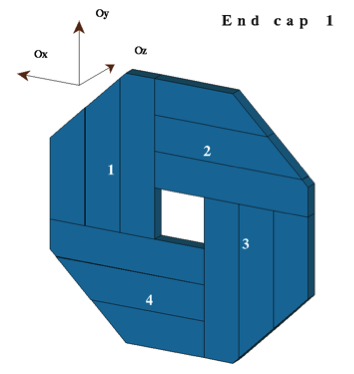
\includegraphics[scale=0.6] {Figures/Calorimetry/SiW_ECAL_EndCaps.png}
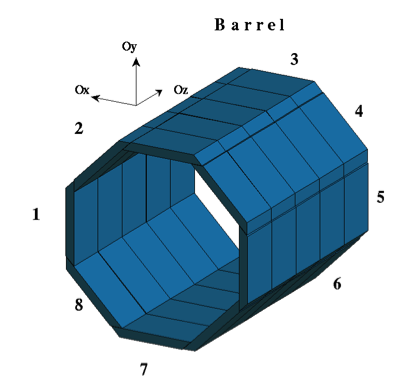
\includegraphics[scale=0.6] {Figures/Calorimetry/SiW-Barrel.png}
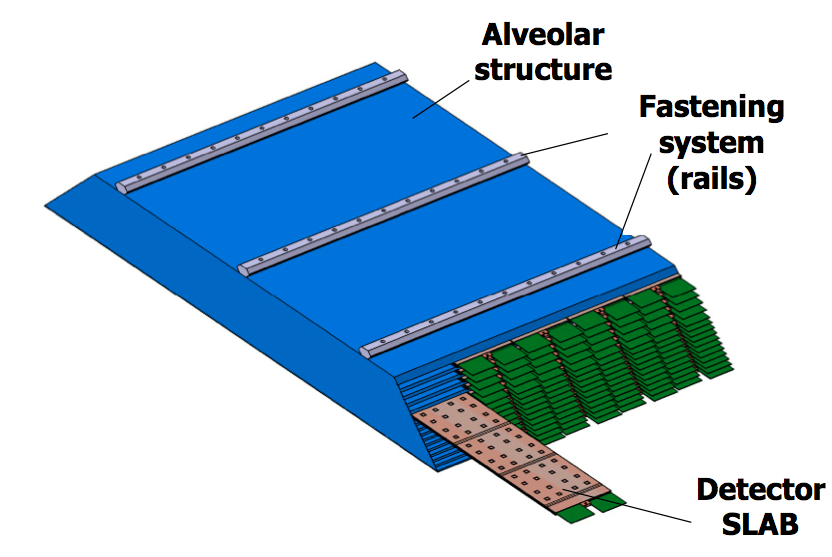
\includegraphics[scale=0.2] {Figures/Calorimetry/SiW-ECAL-Barrel_module.png}
\caption{
  Left: Geometry of the SiW-ECAL Endcaps. %
  Middle: Barrel %
  Right: Geometry of the barrel modules. %
}
\label{fig:Siw_ECAL-geom}
\end{figure}

\paragraph{ECal thickness}

% VBTD: TO BE RECALCULATED WITH CEPC MODULES, IF COOLING...
For a baseline design featuring 30 layers -- split in 2 sections of 20 and 10
layers, holding each an equal amount of $12 Xo$ of W -- $525 microns$ thick wafers,
and a base plate of $20{mm}$ of carbon, the ECal thickness is estimated at
$223??{mm}$.

For a reduced number of layers, at 22 (with section of 14 and 8), but thicker
wafers ($725 microns$), the thickness becomes $191??{mm}$.

\paragraph{ECal dimensions}

% Dimension of small ILD as of Sept. 2017.

The Barrel consist of 8 staves of 5 trapezoidal modules. %
Each barrel module contains 5?? columns of alveoli. %
The number of modules and alveoli is even in order to avoid any special region
at the azimuthal angle $theta=0$. %
%VBTD Check coordinate system in global document
The alveolus size is fixed to $186 {mm}$ by mechanical limits and by cost
optimisation considerations, to contain exactly two 6-inch wafers or
one-and-a-half 8-inch wafer. %
Integrating the alveolus size, walls of modules and contingencies, the barrel
length amount to $4700 {mm}$. ($4900{mm}$ in CEPC simulations). %
A gap of typically $70 {mm}$ ($100{mm}$ in simulation) is left between the
barrel sides and end-cap front parts, whose precise dimension will depend on the
amount of ancillaries needed to service the ECAL and trackers (power and DAQ
cables, cooling pipes, patch panels).

The end-caps are made of quadrants of 2 modules of 4 and 3 alveoli columns.  %
Their inner radius is fixed by the ECal ring at $400{mm}$. %
With 7 alveoli columns, the end-cap outer radius is $1755 {mm}$. %
An overshoot of $32 {mm}$ is left between the outer radius of the barrel and
of the end-caps, in order to contain the EM shower impinging the region of
overlap. see figure~\ref{fig:SiW-ECAL_PhiScan}. %
This fixes the inner radius size of the ECal barrel at $1498 {mm}$ or
$1530{mm}$. %

\begin{figure}[tbp]
\centering
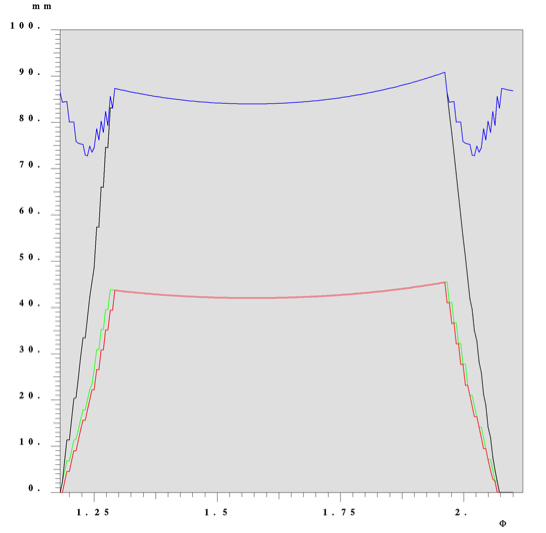
\includegraphics[scale=0.50] {Figures/Calorimetry/SiW_ECAL_X0_PhiScan.png}
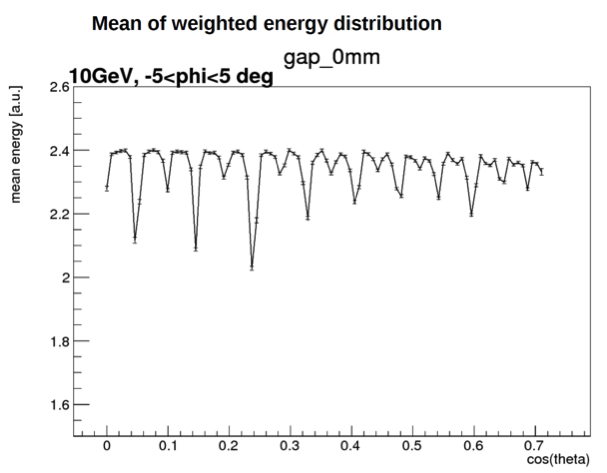
\includegraphics[scale=0.70] {Figures/Calorimetry/SiW-ECAL_Theta_Scan.png}
\caption{ %
  Left: Thickness of Tungsten seen as function of the polar azimuthal angle scan
  of one octant of the barrel.  %
  Right: Mean Theta angle scan }
\label{fig:SiW-ECAL_PhiScan}
\end{figure}

For such a geometry, % C-x * d command for emacs-calc embedded
% [calc-mode: justify: left]
% [calc-mode: language: normal]
% cols := 8*5*5 + 2*4*7 =>
% slabsS := cols * 22 =>
% slabsL := cols * 30 =>
summing the barrel (200) and end-caps (56), 256 alveoli columns are needed.  %
For 22 (resp. 30) layers, and this yields 5632 (7680) alveoli, and as many
detector slabs.

\paragraph{Slab geometry}
In each alveola of the modules, a slab is inserted.  %
Slabs contains 2 symmetric layers of Silicon sensors glued on PCB, equipped
with readout ASICs, high voltage distribution by a Capton foil and copper layers
for passive cooling. %
The elements are chained on both sides of a Carbon fibre cradle taking the shape
of an H, with a core of Tungsten, and shielded by an aluminium cover. %
This so-called H-Structure is illustrated below.
\begin{figure}[tbp]
\centering
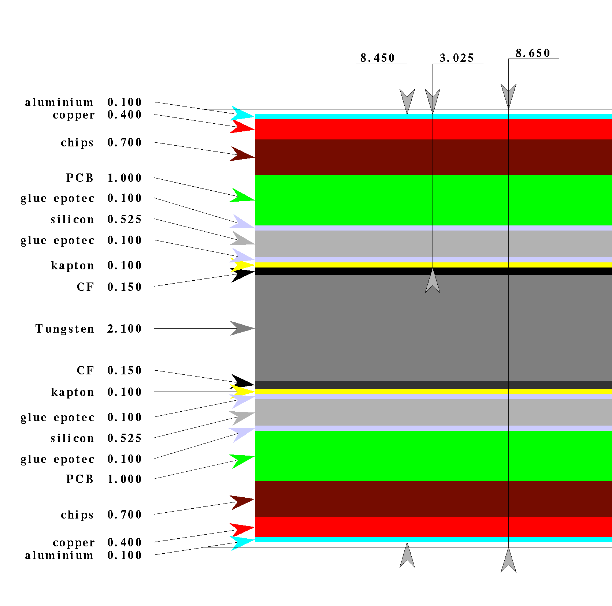
\includegraphics[scale=0.8] {Figures/Calorimetry/SiW-ECAL-Alveola_cut_525.png}
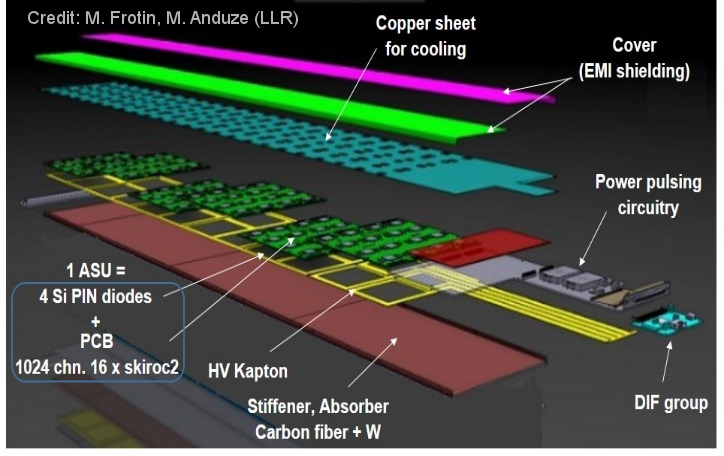
\includegraphics[scale=0.8] {Figures/Calorimetry/SiW-ECAL-Long_SLAB_eclate_sign_v2.png}
\caption{ %
  Left: Transverse cut through of a thin layer of the SLAB. %
  Right: Exploded view of the top layer of a slab of the SiW-ECAL. %
  The same structure is mirrored below the slab.  %
}
\label{fig:Siw_ECAL-Slab}
\end{figure}

To insure scalability and industrial production, the design has been made as
modular as possible: the basic unit is the ASU (Assembly Single Unit), made of a
$18�18{mm�}$ PCB onto which 4 wafers of $90�90{mm�}$ wafers are glued.  %
Each ASU would handle 256 cells with 4 ASICs, for cell surfaces of %
% 180 / 16 => 11.25
$11.25�11.25{mm�}$.

The ASUs are chained together for the clock and configuration distribution and
data collection. %
For a radius of %RinnerB%
$1498{mm}$ the longest (shortest) barrel slabs
measure %RinnerB * 2 * sin (Pi/8)
$1146{mm}$ ($955{mm}$). % short = long - ECAL thickness
In the end-caps, these number are ??, ??.

%In total ?? (?? )ASUs, ?? (??) {m�} of silicon, ?? (??) chips and ?? (??)
%ASICs assuming 64 channels per chip must be produced.

\subsubsection{Electronics}

One of the most critical element of the CEPC calorimeters is the readout
electronics which is defined by the dynamic range, the effective digitisation,
mode of trigger, the rate of working and power consumption per channel.

%\subsubsection{Dynamic range}
%\label{sec:SiW-DynRange}

{\bf {Dynamic range:}} A MIP going through a 725{$microns$} diode would produce % 80 * 750 = 60000
$\simeq 60000 $ electron-pairs holes or % * 1.6e-19 = 9.6 e-15
a charge of $9.6{fC}$?? as the most probable value (MPV). %
To record MIPs with an efficiency higher than 95\% this ports the low-end of the
dynamic range to a 1/3 of the MPV.  %
The high-end is determined by the number of MIP equivalent at the core of the
high-energy EM showers, which can reach up-to 10000 MPV or $96{pC}$ for
$11�11{mm�}$ cells. %
%If the typical precision aimed at for the calibration using MIPs is of the
%percent, one should expect 20-100 adcc at the MPV and
% VBTD: TO BE X_CHECKED
%full digital dynamic range of $10^6$, or 18-20 bits (maybe reduced to 16 using
%multiple dynamic ranges).

%\subsubsection{Timing}
%\label{sec:SiW_ECAL_timing}

{\bf {Timing:}} Time measurement of deposits in the calorimeters can be useful to Particle Flow
algorithms to help disambiguate particle contributions.  For the CMS HGCAL it is
planned to distinguish particle stemming from different
interactions~\cite{Magnan:2017exp}, by achieving a timing of $50-20{ps}$ on
EM showers.  %
For $e^+e^-$ colliders, with a single primary vertex, precision timing of
individual cells -- or group of cells -- could still be useful to reduced the
confusion and improve the resolution.  The required precision is uncertain and
should be studied further. %
Recent version of the SKYROC2a ASIC, could be operated~\cite{Suehara:2017} on
test board with a measure of time close to 1.4{ns}.  The performance has to be
measured in an integrated design. %

%\subsubsection{Rates}

%As a circular collider, the CEPC will run continuously with 2 bunches separated
%by $3.6??\u{\us}$ at the highest energy and ?? bunches separated by $??\u{\us}$
%in the high luminosity run.  %

{\bf {Rates:}} The running conditions a circular collider preclude any pulsed operation as is
planned for the linear ones, where clocks, pre-amps, digital conversion are
powered sequentially at a few Hz. %
A partial in-time shut-off or local on-demand switch-on of the ADC and TDC parts
can be envisaged, leaving the pre-amp as the single major power consumer.
% VBTD: check number for Klaus chip
% VBTD: to discuss with Stephane
As a point of reference, the current power consumption for SKIROC2 chips
designed for the SiW-ECAL of ILD is of $5{mW}$ per channel in continuous mode.


%\subsubsection{Occupancy}
%\label{sec:SiW-Occupancy}

{\bf {Occupancy:}} The occupancy of the calorimeters should be very low.
% VBTD NUMBERS, NUMBERS, NUMBERS!!!
This pushes in the the direction of designing pre-amps with a very small
consumption when there is no signal.



%\subsubsection{Ancillaries}

\subsubsection{Power \& Cooling}
\label{sec:SiW-Power}

To the first order, the amount of power dissipates scales with the number of
electronics channels.  One important issue is to decide on the power scheme:
\begin{itemize}
\item a reduced number of channels using only passive cooling at the heart of
  the detector, such as planned at the ILD; a $400{microns}$-thick copper sheet
  will drain the heat to the end of the slab, where it is removed by a cooling
  system.
\item keep a high granularity but include $\mathrm{CO}_2$ cooling in the
  absorbers such as envisaged for the HGCAL.
\end{itemize}

The CEPC ECAL is at edge of both options, with a limit for the purely passive
option of the order of $2�2{cm�}$ cells for a increase of temperature limited
to $\Delta T \sim 10{^{\circ} C}$ at the remote-end of the slab.

\paragraph{Water cooling}

Current plans for the ILD SiW-ECAL is to use a leak-less water cooling system to
extract the heat at the end of each slab from the copper. %
Details of implementation can be found in~\cite{Grondin:2017qzp, Grondin:2017}.

\paragraph{CO$_2$ cooling}

HGCAL is preparing a biphasic CO$_2$ cooling system, with pipes circulating
inside the absorber planes, made of an alloy of Tungsten and Copper.  %

A similar system adapted to the SiW-ECAL has been simulated~\cite{boudry:2014}.
The ILD $400 microns$ passive colling are replaced by plates of $3{mm}$ of Copper,
equipped with $1.6{mm}$ inner-diameter pipes for CO$_2$ circulation, glued on
the ASICs, on both side of the slab. %
\begin{figure}[tbp]
\centering
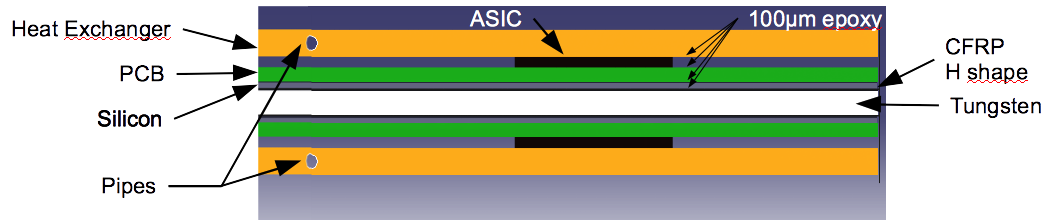
\includegraphics[width=12cm] {Figures/Calorimetry/SiW-ECAL-CO2_slab_section.png}
\includegraphics[width=12cm] {Figures/Calorimetry/SiW-ECAL-CO2_Module_ThermAll.png}
\includegraphics[width=12cm] {Figures/Calorimetry/SiW-ECAL-CO2_Module_ThermExch.png}
\caption{ %
  Top: Transverse section of slab equipped with CO$_2$ cooling pipes embedded in the
  cooling plates %
  Left: Heat map over the full module. %
  Right: heat map in the heat exchanger %
}
\label{fig:Siw_ECAL-Slab-cooling}
\end{figure}
Assuming a fully transversally isolated system, with ASICs a sole heat source at
equilibrium dissipating $0.64{W}$ ($10{mW}$ per channel times 64 channels),
and a fixed working point of $20^{circ}C$ for CO$_2$ (i.e assuming perfect heat
absorption), a doubled sided module of $252�252{mm^2}$ holding 32 chips cooled
by $2�2$ pipes was simulated.

% Heat conductivity are best guess only: Epoxy ~
% $0.795 W/m K Composite highly anisotropic (high along fibres) PCB are
% laminated of 3% of Cu (385W/m.K) + 97% of FR4 (0.3W/m.K)
% ASICs package choosen as 1 W/m.K

Very preliminary simulations in "ideal conditions" show a difference of $\Delta T
\sim 2^{circ}C$ mostly centered on ASIC's
($0.3^{circ}C$ in the exchanger itself only).  %

%\subsubsection{Cost issues}

%Silicon price

%Radius

%number of layers

\subsubsection{Status of R\&D}

%\subsubsection{CALICE}
%\label{sec:CALICE}

The performances of a Silicon-Tungsten ECAL have beed explored using the
``physical prototype'' of the CALICE collaboration, on numerous beam tests
during the years 2005-2011~\cite{Je,Adloff:2009zz,Poschl:2012be}.

Some ASU, similar to the one foreseen for the ILD detector have been operated in
two beam test campaigns: first at CERN in 2015, where 3 ASU mounted on test
boards behaved as expected~\cite{Balagura:2017pka}; a signal to noise ratio
(SNR) - defined as the Most Probable Value of a Landau fit on data, divided by
the Gaussian width of the noise -- reached typical values of 15-18, with a very
limited number of masked channels.

More recently a campaign at DESY using 1-5 GeV electrons, punching through
``short slabs'', featuring all the elements of the slabs described in
section~\ref{sec:SiW-Geom} but limited to a single ASU on a single side, could
reach a SNR of $\simeq 20$ in average~\cite{CHEF_Irles:2017}.  \\

The collected data is still under analysis for estimated calorimetric
performances, but they are expected to be similar to the physics prototype.

%\subsubsection{Long SLAB design}

The building of a ``long slabs'' is being actively pursued, and should be
completed toward the end of year 2019; the R\&D involves all the power, cooling
and FE issues for an ILD near the ILC.

The results and design will have to be adapted for a circular collider, where
operation {\it a priori} forbid power-pulsed operations.


\subsection{Scintillator-Tungsten Sandwich Electromagnetic Calorimeter}
TBD by Zhigang Wang and Yunlong Zhang ...

%%%%\\\\\\\\\\\\\\
\section{Hadronic Calorimeter for Particle Flow Approach}
%
\subsection{Introduction}
High-granularity hadronic calorimeter concept is to play an essential role in PFA-based experiments such as
CEPC. It allows to separate the deposits of charged and neutral hadrons and to precisely measure the energy of
the neutrals. The contribution of the neutrals to the jet energy, around 10\% on average, fluctuates in a wide
range from event to event, and the accuracy of the measurement is the dominant contribution to the particle
flow resolution for jet energies up to about 100~GeV. For higher energies, the performance is dominated by
confusion, and both topological pattern recognition and energy information are important for correct track
cluster assignment. High-granularity hadronic calorimeter is thus needed to achieve excellent jet energy
resolution.

HCAL are sampling calorimeters with steel as absorber and scintillator tiles or gaseous devices with embedded
electronics for the active part. The steel was chosen due to its rigidity which allows to build self-supporting
structure without auxiliary supports (dead regions). Moreover, the moderate ratio of hadronic interaction length
($\lambda_{I}=17$~cm) to electromagnetic radiation length ($X_{0}=1.8$~cm) of iron, allows a fine longitudinal
sampling in terms of $X_{0}$ with a reasonable number of layers in $\lambda_{I}$, thus keeping the detector
volume and readout channel count small. This fine sampling is beneficial both for the measurement of the sizable
electromagnetic energy part in hadronic showers as for the topological resolution of shower substructure, needed
for particle separation.

The active detector element has very finely segmented readout pads, with $1\times1$~cm$^2$ size, for the entire
HCAL volume. Each readout pad is read out individually, so the readout channel density is approximately
$4\times10^5$/m$^3$. For the entire HCAL, with $\sim$100~m$^3$ total volume, the total number of channels will be
$4\times10^7$ which is one of the biggest challenges for the HCAL system. On the other hand, simulation suggests
that, for a calorimeter with cell sizes as small as $1\times1$~cm$^2$, a simple hit counting is already a good
energy measurement for hadrons. As a result, the readout of each channel can be greatly simplified and just
record 'hit' or 'no hit' according to a single threshold (equivalent to a '1-bit' ADC). A hadron calorimeter
with such kind of simplified readout is called a Digital Hadron Calorimeter (DHCAL). In a DHCAL, each readout
channel is used to register a 'hit', instead of measure energy deposition, as in traditional HCAL. In this
context, gas detectors (such as RPC, GEM) become excellent candidates for the active element of a DHCAL.
Another technology option is Analog Hadron Calorimeter (AHCAL) which is based on scintillator with SiPM as active sensor.


A drawing of the HCAL structure is shown in Figure~\ref{fig:441}, the barrel part is made of 5 independent and
self-supporting wheels along the beam axis. The segmentation of each wheel in 8 identical modules is directly
linked with the segmentation of the ECAL barrel. A module is made of 40 stainless steel absorber plates with
independent readout cassettes inserted between the plates. The absorber plates consist of a total of 20~mm
stainless steel: 10~mm absorber from the welded structure and 10~mm from the mechanical support of the detector
layer. Each wheel is independently supported by two rails on the inner wall of the cryostat of the magnet coil.
The cables as well the cooling pipes will be routed outside the HCAL in the space left between the outer side
of the barrel HCAL and the inner side of the cryostat.

%
\begin{figure}[tbp]
\centering % \begin{center}/\end{center} takes some additional vertical space
\includegraphics[width=7.cm]{Figures/Calorimetry/441_1.jpg}
\includegraphics[width=7.cm]{Figures/Calorimetry/441_2.jpg}
\caption{\label{fig:441} Longitudinal profile (Left) and transverse section (Right) of the HCAL.}
\end{figure}
%

%%%%\\\\\\\\\\\\\\
\subsection{Semi-Digital Hadronic Calorimeter (SDHCAL)}

\subsubsection{Introduction}

For the CEPC  we propose the use of gaseous detectors for the HCAL active layers: The Glass Resistive Plate Chambers (GRPC).  This is motivated by the excellent efficiency and very good homogeneity the gaseous detectors could provide.  Another important advantage of  gaseous detectors is the possibility to have very fine lateral segmentation. Indeed, in contrast to scintillator tiles,  the lateral segmentation of gaseous devices is determined by the readout electronics and not by the detector itself.  Active layer thickness is also of importance for what concerns the CEPC hadronic calorimeter to be placed inside the magnetic field. Highly efficient gaseous detectors can indeed be built with a thickness of less than 3 mm. Other gaseous detectors could achieve such performance. However, GRPC detectors have the advantage of being cost-effective and discharge free. They are also known for their fast timing performance which could be used to perform 4D construction of the hadronic showers. Such a construction can improve on hadronic showers separation by better associating the energy depots belonging to the same shower from those of other showers. It can also improve on the energy reconstruction by identifying the delayed neutrons and assigning them a different weight.

To obtain excellent  resolution of hadronic shower energy measurement a binary readout of the GRPC is the simplest and most effective scenario. However,  a lateral segmentation of a few millimeters is needed to ensure good linearity and resolution of the reconstructed energy. Such a lateral segmentation leads to a huge number of electronic channels resulting in a complicated readout system design and a too large power consumption.  1x1 cm$^2$ cells are found to be a good compromise that  still provides a very good resolution at moderate energies.  However, simulation studies show that  saturation effects are expected to show up  at higher energies ($\mathrm{> 40\,GeV}$). This happens when many particles cross one  cell in the center of the hadronic shower.  To reduce these effects, the choice of multi-threshold electronics (Semi-Digital) readout is chosen to improve on the energy resolution by exploiting the particle density in a more appropriate way. These elements were behind the development of a Semi-Digital Hadronic CALorimeter (SDHCAL) that we propose to equip one of the CEPC future experiments.

Even with a 1x1 cm$^2$ lateral granularity of the readout system, a huge number of electronic channels is still needed. This has two important consequences.  The first is the power consumption and the resulting increase of temperature which affects the behavior of the active layers. The other consequence is the number of service cables needed to power, read out these channels. These two aspects can deteriorate the performance of the HCAL  and destroy the principle of PFA if they are not addressed properly.

The R\&D pursued by the CALICE SDHCAL groups has succeeded to pass almost all the technical hurdles of the PFA-based HCAL. The SDHCAL groups have succeeded to build the first technological prototype \cite{SDHCAL} of these new-generation calorimeters with 48 active layers of GRPC, 1m$^2$ each. The prototype validates  the concept of high-granularity gaseous detector and permits to study the energy resolution of hadrons  one can obtains with such calorimeter.


\subsubsection{Readout electronics}

To read out  the SDHCAL an ASIC called HARDROC2 was developed.  To solve the problem of connections related to the high number of electronic channels, the option of a detector embedded electronics  using the DAISY chain scheme was chosen and Printed Circuit Board (PCB) were conceived for the readout of large detectors GRPC.

%\subsubsection{ Front-end ASIC}

- {\bf Front-end ASIC}: The HARDROC2 chip (HR) implements a multi-threshold readout which integrates the functionalities of amplification, shaping, digitization, internal triggering and local storage of the data.  Each of its 64 channels consists of a fast low impedance current preamplifier with 8-bit variable gain (in the $[0,2]$ range) followed by 3 fast shapers (15~{ns} shaping time). A low offset discriminator is present on each path and the three corresponding thresholds establish the multi-level readout.  The thresholds are set using three integrated 10-bit Digital to Analog Converters (DAC). The outputs of the three discriminators are then encoded and stored in an internal digital memory latched by a trigger event.  A trigger is generated when one of the lowest level discriminators is fired but can also be configured on the other thresholds.  A frame consists of the 64 encoded discriminator outputs, plus a 24-bit time-stamp and a chip identifier is stored after a trigger is received.
Noisy channels could be easily masked via the configuration parameters control.  In order to avoid fake triggers produced by noisy channels, the output of each discriminator can be switched off from the trigger generator logic via the configuration parameters control (Slow Control hereafter) commands.  The response of all the channels can be calibrated by injecting an analog signal through an integrated 2$\pm$0.02~{pF} input test capacitor; this is a useful tool to make the response of the different channels as uniform as possible~\cite{small}.
The ASIC contains a 127-frame long digital memory. This allows to work in a triggerless mode and keep all the data accumulated during the bench crossing.

Once the memory is full the acquisition is stopped, the  readout is performed and the ASIC can start acquisition again.  The Gray-coded time-stamp is derived from an external 5~{MHz} clock.
 An essential feature of the HR is the possibility to be operated in the power-pulsing mode (PP) that consists of switching off almost all power-consumption functionalities in between the bench crossings (BC) of the electron beams. In the case of CEPC this mode may allow a moderate reduction of the power consumption but this is not enough to prevent the detector heating due to the power consumption. Therefore an embedded active cooling system is needed.

%\subsubsection{Active Sensor Units}

- {\bf Active Sensor Units}: To read out the  1~{m}$^2$ detector of the SDHCAL prototype, an electronic board with the same size is needed.  This electronic board is an important piece in the present design. It hosts both the pick-up pads and the ASICs in addition to the connections between the pads and the ASICs and those linking the different ASICs.   To ensure good transmission qualities and low cross-talk,  50 cm $\times$ 33 cm,   8-layer Printed Circuit Board (PCB) is designed. Each of these ASUs hosts 24  chips to read out 48$\times$32 pads of 1cm $^2$ each.  This dressed PCB is dubbed Active Sensor Unit (ASU). The routing of each input signal from its own pad up to chip pin has been carefully optimized to reduce the cross-talk.
The rooting was conceived so two of the ASUs can be associated to form one slab hosting 48 ASICS.  Each slab is then connected to one Detector InterFace board (DIF). The connection  between the DIF and  the slab as well as the connection of the two ASUs  is performed   thanks to  tiny connectors  allowing the different clocks, signals as well as the power to circulate between the two  ASUs.  Three slabs are then assembled  to form the required electronics board. To ensure the same electric reference level for the  six ASUs, the GND layer of the six ASUs is connected thanks to a copper gasket on all the common sides.   Similar schemes could be proposed for GRPC detectors with larger size.

%\subsubsection{Front-end and back-end boards}

- {\bf Front-end and back-end boards}: The interface between the ASUs and the data acquisition system (DAQ) is realised by the DIF. The main elements of the DIF is an FPGA and USB, HDMI and SAMTEC connectors. It manages the control signals (\textit{e.g.} clock, busy/ready, external/internal trigger, power-pulsing) and supply power to the ASICs and also performs the readout of the ASIC memories. DIFs are read out by other FPGA-based boards called Data Concentrator Cards (DCC). They can be connected up to 9 DIFs through HDMI links and are controlled by a synchronous DCC (or SDCC). The SDCC can connects to up to 9 DCCs to which it distributes the clock and the commands. It is also connected to the computer network for the user to control the DAQ.

%\subsubsection{ Acquisition software}
- {\bf Data Acquisition software}: To exploit the data collected by  the SDHCAL detectors an acquisition software was developed. This software is organized in three parts. The first one allows to access the hardware devices (DIF, SDCC) through an FTDI chip associated to each of these devices. It transmits the configurations parameters to ASICs through these devices and collect the data as well. The second part is the configuration data base. It gives the possibility to store and retrieve all parameters needed by the DAQ system. The database itself is hosted on an Oracle server. To interface this SQL database with the DAQ software and to allow users to insert and query data without knowledge of SQL, a C++ library has been written. A special care was taken to allow to download the parameters associated to a given parameters of the prototype (roughly 550000 parameters) in few seconds. The third part concerns  the data collection.  Data from different DIFs may be readout at a different times but will have the same Bench Crossing IDentifier (BCID) for a given trigger. The logical way to keep synchronicity is to store in a BCID indexed map the buffers of all read DIFs but it requires to man-age memory allocation, access and cleaning. This was achieved thanks to the abilities offered by recent Linux kernels to use file based shared memory.  In addition, whenever several computers are involved in the data taking, as it is the case for the SDHCAL prototype,  a communication framework is needed. The CMS data acquisition XDAQ framework was chosen. This provides  communication tools, an XML description of the computer and software architecture, a web-server implementation of all data acquisition application and a scalable event builder. A monitoring system was also developed to have an online follow-up of the acquisition during data collection.

\subsubsection{Detector development}

The structure of GRPC proposed as an active layer of the HCAL proposed for CEPC is shown in Figure~\ref{chamber}. It is  made out of two glass plates of 0.7 mm and 1.1 mm thickness.  The thinner is used to form the anode while the the thicker forms the cathode. Ceramic balls of  1.2 mm diameter are used as spacers between the glass plates.  The balls are glued on only one  of the glass plates.  In addition to those balls,  13 cylindrical fiber-glass buttons of 4 mm diameter are also used.  Contrary to the ceramic balls the buttons  are glued to both plates ensuring thus a robust structure. Special spacers (ceramic balls) were used to maintain uniform  gas gap of 1.2 mm. Their number and distribution were optimized to reduce the noise and dead zones ($0.1 \%$).

The distance between the spacers (10 cm)  was fixed so that the deviation of the gap distance between the two plates under the glass weight and the electric force does not exceed 45 microns.  The choice of these spacers rather than fishing lines was intended to reduce the dead zones ($0.1 \%$).  It was also aimed at reducing the noise contribution observed along the fishing lines in standard GRPC chambers.  The gas volume is closed by a 1.2 mm thick and 3 mm wide glass-fiber frame  glued on both glass plates. The glue used for both the frame and the spacers was chosen for its chemical passivity and long term performance.  The resistive coating on the glass plates which is used to apply the high voltage and thus to create the electric field in the gas volume was found to play important role in the pad multiplicity associated to a mip \cite{small}. A product  based on colloids containing graphite was developed. It is  applied on the outer faces of the two electrodes using the silk screen print method, which ensures very uniform surface quality. The measured surface resistivity at various points over a 1m$^2$ glass coated with the previous  paint showed a mean value of 1.2 M$\Omega/\square$ and a ratio of the maximum to minimum values of less than 2 ensuring a good homogeneity of the detector.

Another important aspect of this development concerns the gas circulation within the GRPC taking into account that for the CEPC SDHCAL,  gas outlets should all be on one side.  A genuine system was proposed. It is based on channeling  the gas along one side of the chamber and releasing it into the main gas volume at regular intervals. A similar system is used to collect the gas on the opposite side.  A finite element model has been established to check the gas distribution. The simulation confirms that the gas speed is reasonably uniform over most of the chamber area.
The GRPC and its associated electronics are housed in a special cassette which protects the chamber and ensures that the readout board is in intimate contact with the anode glass. The cassette is a thin box consisting of 2.5 mm thick  stainless steel plates separated by 6 mm wide stainless steel spacers. Its plates are also a part of the absorber.

The electronics board is assembled thanks to a polycarbonate spacer which is also used to fill the gaps between the readout chips and to improve the overall rigidity of the detector. The electronics board is fixed on the small plate of the cassette.  Thanks to tiny screws and the new set is fixed on the other plate which hosts the detector and the spacers. The whole width of the cassette is 11 mm with only 6 of them corresponding to the sensitive medium including the GRPC detector and the readout electronics.


\begin{figure}
\centerline{\includegraphics[width=0.70\columnwidth]{Figures/Calorimetry/chamber}}
\caption{Cross-section through a 1~m$^2$ chamber.}\label{chamber}
%\end{wrapfigure}
\end{figure}

\subsubsection{SDHCAL technological prototype}

An SDHCAL prototype fulfilling the efficiency, robustness and the compactness requirements of the future PFA-based leptonic collider experiments~\cite{SDHCAL} was built. 48 cassettes as the one described above were built. They fulfilled a stringent quality control.   It is worth mentioning that 10500 HR ASICs were produced and tested using a dedicated robot for this purpose. The yield was found to be higher than 92\%.  The ASICs were then fixed on the PCBs to make a 1m$^2$ and itself fixed on the cassette cover once successfully tested.    The cassettes were inserted in a self-supporting mechanical structure that was conceived and built  in collaboration with the Spanish group of CIEMAT. The structure is made of Stainless Steel plates of 1.5 cm each. The plates were machined to have an excellent flatness and well controlled thickness. The flatness of the plates was measured using a laser-based interferometer system. It was found that the flatness of  the plates are less than 500 microns. This results guarantees that for the SDHCAL V structure proposed for ILD, a tolerance of less than 1mm is achievable.
The prototype construction  lasted less than 6 months. A commissioning test at CERN in 2011 allowed to understand the whole system behavior.
In April 2012 the prototype was exposed to pion, muon, electron beams of both the PS and the SPS of CERN Figure (\ref{Prototype}). Power-pulsed mode was applied to the whole prototype using the beam cycle structure (0.3 ms time duration for the PS beam and 9 s for the SPS beam every 45s).
The data were collected continuously in a triggerless mode.
Figure~\ref{Eff} shows the efficiency (left) and pad multiplicity (right) of the prototype's GRPC chambers measured using the muon beam. Figure~\ref{pion} shows a display of two events collected in the SDHCAL. One is a produced by a pion interaction (left) and the other by an electron interaction (right).

The SDHCAL prototype  results obtained  with  a minimum data treatment (no grain correction) show clearly that excellent linearity and good resolution~\cite{FirstResults} could be achieved on large energy scale as can be shown in Figure~\ref{Linearity} where results obtained in two different beam lines are obtained using the same detector configurations.  Useless to mention that the high granularity of the SDHCAL allows one to study thoroughly  the hadronic showers topology and to improve on the energy resolution by, among others,  separating the electromagnetic and the hadronic contribution.  The separation between close-by showers will also get big benefit thanks to the high granularity on the one hand and to to the very clean detector response ( < 1 Hz/cm$^2$) on the other hand. The results obtained with the the SDHCAL~\cite{Remi} confirm the excellent efficiency of such separation thanks to the SDHCAL performance.    In addition, the high-granularity of the SDHCAL allows to extract the track segments of hadronic showers in a very efficient way~\cite{Hough}. The track segments (Figure~\ref{Hough}) are then used to study the detector behavior in-situ. This  is a simple but powerful control and calibration tool for a running calorimeter.

The quality of data obtained during several campaigns of  data taking at the CERN PS and SPS beam lines validates completely the SDHCAL concept.  This is especially encouraging since no gain correction was applied to the electronics channels to equalize their response. Still, improvement was further  achieved by applying gain and threshold correction schemes in terms of  the calorimeter response homogeneity.

A digitizer describing the response of the  GRPC within the SDHCAL was developed~\cite{Digitizer}. It allows to study the SDHCAL behavior in a realistic manner in the future experiments.

In parallel to the prototype construction, a single cassette was tested in a magnetic field of 3 Tesla (H2 line at CERN) applying the power-pulsed mode.  The TB results~\cite{PP} indicated clearly that the use of the power-pulsed mode in such a magnetic field is possible. The behavior of the detector (efficiency, multiplicity..) was found to be similar to those obtained in the absence of both the magnetic field and the power-pulsed mode.

\subsubsection{Preparation for future experiments}

A genuine self-supporting mechanical structure to host the hadronic calorimeter of future PFA-based leptonic collider experiments was fully studied.   The structure (called V-structure) was conceived to eliminate the projective holes and cracks so none of the particles produced close to the detector centre could escape detection. The V-structure has additional advantages. It eliminates in principle the space between the barrel and the Endcaps avoiding the shower deformation which results  not only  because of  this space but also  of the different cables and services needed in CMS-like mechanical structures.  In this structure the different services such as  the gas tubes, data collection and electric cables of both the barrel and the Endcaps are taken out from the outer radius side.Detailed studies have shown that the deformation of this structure is extremely low and its robustness was verified experimentally with the SDHCAL technological prototype built with a self-supporting structure respecting the spirit of the V one.  Services and  Integration issues were also worked out.  Besides, realistic costing was performed , based on the prototype experience.

\begin{figure}
\centerline{\includegraphics[width=0.50\columnwidth]{Figures/Calorimetry/prototype.JPG}}
\caption{The SDHCAL prtototype in beam test at CERN.}\label{Prototype}
%\end{wrapfigure}
\end{figure}



\begin{figure}[htp]
\begin{center}
\includegraphics[width=0.45\textwidth]{Figures/Calorimetry//Eff.pdf}
\includegraphics[width=0.45\textwidth]{Figures/Calorimetry//Mult.pdf}

\caption{ Left: Efficiency of the GRPC detectors of the SDHCAL. Right: the pad multiplicity of the GRPCs. One third of the chamber 42 was not instrumented.}

\label{Eff}
\end{center}
\end{figure}


\begin{figure}[htp]
\begin{center}
\includegraphics[width=0.45\textwidth]{Figures/Calorimetry/pion.pdf}
\includegraphics[width=0.45\textwidth]{Figures/Calorimetry/electron.pdf}
\caption{ Left: event display of an 70 GeV pion interaction in the SDHCAL prototype. Right: Event display of a 70 GeV electron interaction in the SDHCAL prototype.}
\label{pion}
\end{center}
\end{figure}


\begin{figure}[htp]
\begin{center}
\includegraphics[width=0.45\textwidth]{Figures/Calorimetry/Linearity.pdf}
\includegraphics[width=0.45\textwidth]{Figures/Calorimetry/Resolution.pdf}
\caption{ Left:  a) Reconstructed energy of the hadronic showers collected in both H2 and H6 SPS beamlines. b) the relative deviation of the reconstructed energy with respect to the beam energy. Right: Relative energy resolution of the reconstructed hadronic shower.Pion beam of H6 beamline is largely  contaminated by protons at high energy (>50 GeV).}
\label{Linearity}
\end{center}
\end{figure}


\begin{figure}[htp]
\begin{center}
\includegraphics[width=0.6\textwidth]{Figures/Calorimetry/Hough.pdf}
\caption{ A 3D event display of a pion interaction event showing the track segments extracted by applying a hough transform technique.}
\label{Hough}
\end{center}
\end{figure}




\subsubsection{current SDHCAL R\&D}

Large GRPC of 1m$^2$ were developed and built for the technological prototype. However, larger GRPC are needed in the SDHCAL proposed for future leptonic collider experiments.  These large chambers with gas inlet and outlet on one side need a dedicated study to guarantee a uniform gas gap everywhere notwithstanding the angle of the plate. It is necessary also to ensure an efficient gas distribution as it was done for the 1m2 chambers. To obtain this different gas distribution systems were studied. A new scheme with two gas inlets and one outlet was found to ensure an excellent homogeneity of the gas distribution. This system will be used in the near future to build large detectors exceeding 2m$^2$.
The readout of such chambers needs also to be as efficient as the one of the technological prototype 1m$^2$. An upgrade of the HR ASIC allowing larger dynamic range (01-50 pC) was conceived, produced and successfully tested. The new ASIC (HR3) allows to be directly addressed and easily bypassed in case of failure thanks to the I2C protocol. In addition and contrary to the HR2, the 64 channels of the new ASIC are independent which allows a better calibration procedure.  Furthermore, a new interface board (DIF) is conceived to control the ASICs synchronization and data transfer. Indeed, the space left between the active layer of one module and the cryostat maybe very short in future leptonic experiments (< 5 cm).  This means that the DIF components should be optimized to cope with the volume availability. A new design with new functionalities of the DIF is proposed.  A TPC/IP protocol is adopted for data transfer and a TTC one for the clock synchronisation.  A microprocessor implemented on the new DIF is in charge of the communication between the ASICs and the DIF's FPGA. The new DIF shown in Fig.~\ref{NewDIF} is capable to address up to 432 ASIC.  A new PCB design that allows to assemble few boards to cover up to 3 m$^2$ GRPC detector  was also conceived. Care is taken to ensure robust and flexible but still tiny connection between the different PCB to build a large one. Fig.~\ref{NewPCB} shows a picture of such a PCB equipped with the HR3 ASICs.  Finally a new  technique based on electron beam welding is being tested to build a mechanical structure.  This intends to reduce the steel quantity used to assemble the absorber plates while guaranteeing a minimum deformation. First attempts have taken place at CERN recently ~\ref{EBW} and more study is ongoing to determine the best protocol one should follow to obtain optimal results.
Finally, to cope with the heating produced by the embedded readout system in case of limited or even the absence of use of the Power Pulsing system, a new active cooling system is being studied. Figure~\ref{Cooling} shows a study of a water-based cooling system to absorb the excess of heat in the SDHCAL. The cooling system is very simple but very effective as well. It allows to keep the average temperature as well as the temperature dispersion of the GRPC well under control.


\begin{figure}
\centerline{\includegraphics[width=0.60\columnwidth]{Figures/Calorimetry/NewDIF.png}}
\caption{A new Detector InterFace (DIF) allowing to address up to 432 ASICs of 64 electronic channels each. }
\label{NewDIF}
\end{figure}

\begin{figure}
\centerline{\includegraphics[width=0.60\columnwidth]{Figures/Calorimetry/NewPCB.png}}
\caption{A new PCB equipped with he HR3 ASICs. The PCB is 100 cm $\times $ 33.3 cm. Several PCBs could be connected thanks to tiny flexible connectors to read out very large GRPC detectors.}
\label{NewPCB}
\end{figure}


\begin{figure}
\centerline{\includegraphics[width=0.60\columnwidth]{Figures/Calorimetry/EBW.png}}
\caption{A prototype of an SDHCAL mechanical structure assembled using the electron beam welding technique.}
\label{EBW}
%\end{wrapfigure}
\end{figure}

\begin{figure}
\centerline{\includegraphics[width=0.60\columnwidth]{Figures/Calorimetry/cooling.png}}
\caption{Temperature distribution in an active layer of the SDHCAL operated with no power-pulsing. The cooling system is made of a circulating water inside copper tubes in contact with the ASICs.}
\label{Cooling}
%\end{wrapfigure}
\end{figure}

%%%%\\\\\\\\\\\\\\
\subsection{Analog Hadronic Calorimeter based on Scintillator and SiPM}
\par\setlength{\parindent}{2em} A high-granularity hadronic calorimeter plays an essential role in PFA-based experiments such as CEPC. It allows separation of the energy deposits from charged and neutral hadrons. The contribution of the neutrals to the jet energy, around 10\% on average, fluctuates over a wide range from event to event. The HCAL is a sampling calorimeter with steel as the absorber and scintillator tiles with embedded electronics. The moderate ratio of hadronic interaction length (I=17cm) to electromagnetic radiation length (X$_0$ = 1.8 cm) of steel, allows a fine longitudinal sampling in terms of X$_0$ with a reasonable number of layers.\newline

Various calorimetry options are being developed to address challenges from the stringent performance requirements on future lepton collider experiments for precision measurements of the Higgs boson and for searches of physics beyond Standard Model. Within the CALICE collaboration, a large technological prototype using scintillator tiles and SiPMs is currently being built to demonstrate the scalability to construct a final detector via automated mass assembly. Though this prototype is aimed for the future International Linear Collider (ILC), the outcome of CALICE-AHCAL R\&D activities can be an essential input for the conceptual design of the hadron calorimeter system at the future Circular Electron Positron Collider (CEPC).



\subsubsection{AHCAL geometry and simulation }

The AHCAL consists 40 sensitive and absorber layers, and the thickness is about 100cm. The AHCAL barral consists 32 supper module, each super module consists 40 layers, figure\ref{AHCAL-structure} shows the AHCAL structure.   Figure\ref{fig:7side} shows the AHCAL one layer structure. The scintillator tiles wrapped by reflective foil are used as sensitive medium, interleaved with stainless steel absorber. The thickness of active layer is 4 mm to 5 mm, it depend the thickness of scintillator thickness.

\begin{figure}[h!]
\centering
\includegraphics[scale=0.7] {Figures/Calorimetry/AHCAL_structure.jpg}
\caption{Side view of one layer in AHCAL }
\label{AHCAL-structure}
\end{figure}

\begin{figure}[h!]
\centering
\includegraphics[scale=0.7] {Figures/Calorimetry/Side_view_of_AHCAL.PNG}
\caption{Side view of one layer in AHCAL }
\label{fig:7side}
\end{figure}



  The structure of scintillator tiles is shown in Figure \ref{fig:7cellstructure}. A dome-shaped cavity was processed in the center of the bottom surface of each tile via mechanical drilling and polishing. The diameter and height of cavity are 6mm, 1.5mm, respectively, as shown in Figure \ref{fig:7cellstructure} (right). This design of cavity can improve response uniformity and decrease the dead area of HCAL.

\begin{figure}[h!]
\centering
\includegraphics[scale=0.6] {Figures/Calorimetry/Cell_structure.jpg}
\caption{Top view of a detector cell (left) and sectional view of a detector cell with a dome-shaped cavity (right) }
\label{fig:7cellstructure}
\end{figure}

\par\setlength{\parindent}{2em} The AHCAL prototype detector simulated by Geant4 which was encapsulated in toolkit including several models. The detector model used here was CEPC$\_$v1 detector model and the sub detector was SiCal. The geometry information was extract by Mokka at runtime and the generated events was stored in Slcio, which contains primary information regarding the energy deposition, hit position, time and Monte Carlo particle causing the energy deposition. It can read out by Marlin and translate into Root files for analyzing. The ECAL was simulated 30 layers. The HCAL is a structure of 40 active layers interleaved with 20 mm steel absorber plates. Each active layer is assembled from 3mm plastic scintillator, also the readout layer thickness is 2mm PCB, detector cell size is 30$\times$30$\times$3 mm$^3$. And the TCMT, we simulate 20 layers and each layer is the same component and material as HCAL. Their structure is shown in  Figure \ref{fig:2simecalhcal}.\newline

\begin{figure}[h!]
\centering
\includegraphics[scale=0.7] {Figures/Calorimetry/simecalhcal2.jpg}
\caption{The structure of simulated calorimeters which is a part of the simplify geometry. Red part is the ECAL, Blue part is the HCAL, and white part is the TCMT }
\label{fig:2simecalhcal}
\end{figure}


 \begin{equation}\label{first}
  %\int_a^bf(x)dx  %abcd %
   E_{REC} =a\times E_{ECAL}  +b\times E_{HCAl}
 \end{equation}
For getting the resolution of calorimeters (ECAL and AHCAL) which structure was show in figure \ref{fig:2simecalhcal}. Formula \ref{first} is the energy reconstruction formula, the coefficients a and b in this formula represent ECAL and HCAl calibration constant. After optimization, the calibration constants are a=44.4 and b=44.2 respectively which were corrected by energy of 60GeV. Calibration constants can correct the energy leakage from the calorimeters. So it can be used formula \ref{second} for calculating the resolution. The energy resolution result shows in figure \ref{fig:simresult}. For the resolution is better than the result of CALICE, the reason should be simulation ignore the response difference between detector cells. For the energy linearity, the slope value is 0.99, which means the reconstruction energy is essentially linear.

 \begin{equation}\label{second}
  \frac{\sigma}{E} =\frac{ p_0 } {\sqrt{E} }+ p_1  %��/E=p_0/��E+p_1
 \end{equation}


\begin{figure}[h!]
\centering
\includegraphics[scale=0.7] {Figures/Calorimetry/simecalhcal_result.jpg}
\caption{Left figure is energy resolution, right figure is the result of reconstruction energy linearity }
\label{fig:simresult}
\end{figure}



\subsubsection{Plastic Scintillator cell measurement}

The basic tile size was optimized with respect to particle separation capability and found to be 30 $\times$ 30mm$^2$. The simulation results suggest that it is possible to use the detector cells of larger sizes. For example, it will reduce nearly two-thirds electronics channels by using 50 $\times$ 50mm$^2$ size detector cell instead of 30 $\times$ 30mm$^2$ size. Therefore, the construction costs can be greatly reduced if the larger detector cells can meet the physics requirements. Two larger sizes of detector cells were considered. Four kinds of scintillator (BC408) tiles with different sizes were fabricated and tested, and they are 30 $\times$ 30 $\times$ 3mm$^3$, 40 $\times$ 40 $\times$ 3mm$^3$, 50 $\times$ 50 $\times$ 3mm$^3$ and 30 $\times$ 30 $\times$ 2mm$^3$.

  The SiPM is soldered onto a readout Printed Circuit Board (PCB) and the scintillator tile wrapped by ESR reflective foil is directly glued onto the PCB. Such a cavity design provides enough space for the SiPM package and improves collection efficiency of the light produced by incident particles penetrating the tile at different positions. The SiPM is readout by the Hamamatsu electronic readout board (C12332-01) which has the function of temperature compensation. The time instability of signal amplitude (ADC channel) of SiPM is from 17.59$\%$ to 2.38$\%$ in the range of 22$^o$C to 30$^o$C owing to temperature compensation from the board, as shown in Figure\ref{fig:7temperture}.

\begin{figure}[h!]
\centering
\includegraphics[scale=0.5] {Figures/Calorimetry/temperture_response.jpg}
\caption{SiPM signal amplitude varies with temperature, before (left) and after (right) temperature compensation electronics (Hamamatsu C12332-01) }
\label{fig:7temperture}
\end{figure}


\textbf{Uniformity measurement:}A strongly non-uniform tile response can lead to a distortion of the energy reconstruction in a complete calorimeter, and also compromises the calibration of the detector cells based on single particle signals [4]. The response uniformity of a SiPM inside the cavity of a scintillator tile has been measured with a 90Sr source, as shown in Figure \ref{fig:um}. The trigger scintillator (5$\times$5$\times$3mm$^3$) and 90Sr source were fixed. A detector cell, which was mounted on a step motor, can be finely moved between 90Sr source and the trigger scintillator. Uniformity scans were accomplished by horizontally translating the detector cell in a step size of 5$\times$5 mm$^2$. The electronics data acquisition system is shown in Figure \ref{fig:uda}.

\begin{figure}[h!]
\centering
\includegraphics[scale=0.7] {Figures/Calorimetry/uniformity_meas.jpg}
\caption{Setup of uniformity measurement }
\label{fig:um}
\end{figure}

\begin{figure}[h!]
\centering
\includegraphics[scale=0.7] {Figures/Calorimetry/Data_acq.jpg}
\caption{Block diagram of data acquisition }
\label{fig:uda}
\end{figure}

 Three different sizes tiles (30$\times$30$\times$3mm$^3$, 30$\times$30$\times$2mm$^3$ and  50$\times$50$\times$3mm$^3$) were tested by the Hamamatsu MPPC S12571-025P and S13360-025PE. The photosensitive area of module MPPC S12571-025P is 1$\times$1 mm$^2$ containing 1600 pixels, and each pixel is 25 $\mu$m$\times$25 $\mu$m in size. The MPPC S13360-1325PE whose sensitive area is 1.3mm$\times$1.3mm contains 2668 pixels. The spatial distribution of p.e. (photon equivalents) number with different detector cell areas are shown in Figure \ref{fig:1uniformity}. So the p.e. number presents signal amplitude of different tile areas. It can be seen that the number of p.e. in the center area is a little higher than that of the surrounding area because the MPPC is placed in the center area and there is less self-absorption in the area close to the MPPC. The global mean response is around 32.2p.e. and 100$\%$ of the cell area is within 10$\%$ deviation from the mean value for 30$\times$30$\times$3mm$^3$ cell. The global mean response is around 34.29p.e. and 100$\%$ of the cell area is within 10$\%$ deviation from the mean value for 30$\times$30$\times$2mm$^3$ cell. The three detector cells show good response uniformity. The global mean response is around 8.57p.e. and 94$\%$ of the cell area is within 10$\%$ deviation from the mean value for 50$\times$50$\times$3mm$^3$ cell.

\begin{figure}[h!]
\centering
\includegraphics[scale=0.7] {Figures/Calorimetry/uniformity.jpg}
\caption{The uniformity measurement result of 30$\times$30$\times$3mm$^3$(a), 50$\times$50$\times$3mm$^3$(b)and 30$\times$30$\times$2mm$^3$(c)detector cell }
\label{fig:1uniformity}
\end{figure}

\textbf{Cosmic-ray measurement:}
  The cosmic-ray test setup for measuring responses of scintillator cells to muons is shown in Figure \ref{fig:1cosmicmeas} . The detector cell is placed between two trigger scintillators (20$\times$20$\times$3mm$^3$) tiles. A lead is placed between the detector cell and bottom trigger scintillator to select higher energy cosmic ray events. The coincidence of two trigger signals ensures a muon track passing though the detector cell. Four kinds of tiles with different sizes (30$\times$30$\times$3mm$^3$, 40$\times$40$\times$3mm$^3$, 50$\times$50$\times$3mm$^3$ and 30$\times$30$\times$2mm$^3$) were measured.

\begin{figure}[h!]
\centering
\includegraphics[scale=0.7] {Figures/Calorimetry/cosmic_meas.jpg}
\caption{Schematic diagram of cosmic-ray measurement setup }
\label{fig:1cosmicmeas}
\end{figure}
The single photon spectrum of SiPM was used to calibrate the test system, as shown in Figure \ref{fig:1cosmicresult} (left). The cosmic-ray MIP response spectrum is shown in Figure\ref{fig:1cosmicresult} (right). It is fitted by a Landau convoluted with Gaussian distribution.

\begin{figure}[h!]
\centering
\includegraphics[scale=0.7] {Figures/Calorimetry/cosmic_result.jpg}
\caption{Single photon spectrum of MPPC (left) and responses to muons of 30$\times$30$\times$3mm$^3$ detector cell (right)}
\label{fig:1cosmicresult}
\end{figure}

Seven detector cells of different sizes, polishing methods and wrapping foil types were measured and summarized in figure \ref{fig:cosmictable}. The larger the area of the cell is, the less p.e. are detected, and the results of same size cells varied greatly because of the polishing methods. As is shown in the table that the ESR foil performs better than the TYVEK reflective foil. The cell with the size of 30$\times$30$\times$2mm$^3$ detected 33.89$\pm$0.49 p.e. because of the larger photosensitive area of MPPC.

\begin{figure}[h!]
\centering
\includegraphics[scale=0.5] {Figures/Calorimetry/cosmic_result_table.jpg}
\caption{Cosmic-ray measurement results of detector cells with different sizes }
\label{fig:cosmictable}
\end{figure}

\textbf{MIPs Detection efficiency:}
The detection efficiency of 30$\times$30$\times$3mm$^3$ and 50$\times$50$\times$3mm$^3$ were measured by the cosmic ray test. The detection efficiency of 30$\times$30$\times$3mm$^3$ and 50$\times$50$\times$3mm$^3$ cells are 99$\%$, 98.2$\%$, respectively. According the cosmic-ray test result, the detection efficiency of 30$\times$30$\times$2mm$^3$ with S13360-025PE MPPC also can reach to 98%.

Several size plastic scintillator detector cells of AHCAL were tested. The response uniformity, cosmic-ray responses and detection efficiency of detector cells were measured. The good response uniformity and high detection efficiency results show that both 30$\times$30$\times$3mm$^3$ and 50$\times$50$\times$3mm$^3$ cells are acceptable for AHCAL. The size of detector cell will be decided by the simulation result.

\subsubsection{NDL EQR-SiPM for CEPC AHCAL}
SiPM with epitaxial quenching resistors (EQR SiPM) is one of the main SiPM technologies now under development [16,17]. This kind SiPM was developed in China. As shown in Figure\ref{fig:EQRsipm}, each APD cell (pixel) forms a high electric field, composing an enriched region between N-type epitaxial silicon substrate and P++ cap layer, and it employs the un-depleted region in the epitaxial silicon layer below P/N junction as the quenching resistor. Compared to conventional SiPM configurations that employ poly-silicon quenching resistors on the device surface, it is easier to achieve high density and small micro APD cells, thus obtaining a small junction capacitor; it is also easy to realize low resistance for the quenching resistors, simply based on the resistivity of the epitaxial layer and the geometrical scale. As a result, a low RC time constant of the pixel, or a short recovery time and fast counting rate for the EQR SiPM, can be expected. In addition, thanks to the high geometrical fill factor of the EQR SiPM with a high density of micro APD cells, both wide dynamic range and adequate PDE can be realized at the same time, which satisfactorily resolves the conflict between dynamic range and PDE existing in most commercial SiPMs with poly-silicon stripes as quenching resistors.
\begin{figure}[h!]
\centering
\includegraphics[scale=0.6] {Figures/Calorimetry/EQR_SiPM.jpg}
\caption{Schematic structure of EQR SiPM; APD cell consists of N-enriched regions forming high electric fields between the N-type epitaxial silicon wafer and the P++ surface layer, the un-depleted region in the epitaxial silicon layer below the P/N junction as the quenching resistor, and the APD cells are isolated from each other by the Gap depletion region. }
\label{fig:EQRsipm}
\end{figure}

\begin{figure}[h!]
\centering
\includegraphics[scale=0.7] {Figures/Calorimetry/property_SiPM.jpg}
\caption{Characteristics of NDL EQR PS-SiPM. (a) DCR vs over voltages. (b) PDE vs the wavelength of 360nm-600nm at over voltage of 3.7V; peak PDE is at 420nm and is improved with the increase of over voltage as shown in the inset. (c), (d) show the pulse area distribution collected by cathode at the incident light positions of (1200um, 0) and (1200um, 1200um) respectively. Because of the pedestal electronic noise, the pulse area is starting at negative values. }
\label{fig:1property_SiPM}
\end{figure}

\begin{figure}[h!]
\centering
\includegraphics[scale=0.6] {Figures/Calorimetry/Compare_SiPM.jpg}
\caption{Performance compare between EQR SiPM and Hamamatsu MPPC with similarly high micro-cell density. }
\label{fig:1compareSiPM}
\end{figure}

Furthermore, the fabrication technology of NDL EQR-SiPM is simple, it omits the fabrication steps for producing quenching resistors on the surface; thus, the price of NDL EQR-SiPM is low. Its good property and low price can meet AHCAL requirement, and it will be tried to be used on CEPC-AHCAL detector. Figure \ref{fig:1property_SiPM} show some performance of NDL EQR-SiPM, and figure \ref{fig:1compareSiPM} show the performance compare between NDL EQR-SiPM and Hamamastu MPPC.
\newline



\subsubsection{Electronics and DAQ}

\textbf{Front-end electronics ASIC:}
High-density electronics is indispensable to instrumentation of high-granularity calorimetry. An ASIC chip named SPIROC, developed by the OMEGA group, is capable to handle 36 SiPMs. For each channel, it can be operated in an auto-trigger mode and has a dual-gain charge preamplifier with high dynamic range. It allows to measure for each channel the charge from 1 to 2000 photo-electron and the time within 1 ns using a 12-bit digitizing circuit. With one 8-bit 5V input DAC per channel, the bias voltage for each SiPM can be adjusted to reach its optimum. In each channel, there are 16 analogue memory cells that can buffer both charge and timing signals to be digitized afterwards consecutively. The digitization circuit is shared for both charge and timing measurements to minimize the power consumption, which needs to be as low as $25~{\mu}W$ per channel. The latest version SPIROC2E has been improved in many aspects and its packaging has changed to a thinner BGA, which ensures a compact design for HBU and allows better automated mass soldering.

\textbf{HCAL Base Unit:}
A merit of the AHCAL electronics is flexibility. One full AHCAL active layer can be constructed by connecting several base units (namely HBUs) via connectors, each with $12\times12$ channels in a square plate of $36\times36~cm^2$. The exact granularity is being optimized for CEPC to balance between the detector performance and the number of total channels. To achieve a compact HCAL design, the PCB for each HBU should be thin enough and a 6-layer PCB within 1~mm thickness is proved to be feasible.

As a semiconductor detector, SiPM is intrinsically sensitive to environmental changes, especially temperature. Thus each SiPM needs on-site calibration, which requires an on-board LED circuit for each channel. There is an LED circuit at each channel of an HBU, which can emit UV light to a scintillator tile. Using these photons, the gain of a SiPM can be extracted and monitored.

\textbf{Detector interface:}
ASIC chips are controlled by an interface board named DIF (Detector Interface). One DIF board handles a full HCAL active layer (a long slab with up to $6\times3$ HBUs), corresponding to 72 ASICs in total. The expected data rate per DIF can be estimated based on the event rate at HCAL, which depends on the beam structure at CEPC.

\textbf{LED calibration board:}
A dedicated LED calibration board is needed to control all LED circuits in an HCAL active layer. It can send trigger signals for the proper SiPM calibration.

\textbf{Power board:}
SiPM operation relies on a proper reversely bias voltage. Therefore, between power supplies and ASIC chips, a power board is required to distributing the bias voltage to each SiPM. This power board can also play an important role in regulating voltages for protection and smooth working of SiPMs. Like the DIF board, it would be feasible to use only one such board for an active HCAL layer (up to $6\times3$ HBUs).

\subsubsection{DAQ system}\label{daq}

\textbf{DAQ hardware:}
DAQ system is also required to be compatible to the final detector layout, where two hardware parts are essential. One part is so-called LDA (Link to Data Aggregator), which collects all the data via DIFs from active layers in an HCAL segment and transmit them to a back-end PC for further processing or storage. Smart units like FPGAs are equipped on this board for data packaging and transmission. Modern FPGAs integrated with RAMs are an ideal option to have a capability of data buffering and some advanced feature like system on chip.

The other key hardware part is so-called CCC (Clock and Control Card), which provide a global clock signal and synchronize DIFs. Control signals are also sent to DIFs including starting and stopping acquisition.\newline

\textbf{DAQ software:}
The DAQ software is being developed in the framework of EUDAQ supported by AIDA2020, aiming for a generic solution for a combined setup with several detectors, which is important in test-beam activities during the prototyping phase. The latest version EUDAQ2 has made much progress during extensive beam tests for various combinations of detectors and can be considered as a solution for further HCAL prototyping and beam-test campaigns for CEPC.



%%%%\\\\\\\\\\\\\\
\section{Dual-readout Calorimetry}
\subsection{Introduction}

Till now, the performance obtained in hadronic energy measurements has
been by far worse than for the electromagnetic ones, since showers from
single hadrons or jets develop an electromagnetic component ($em$
fraction, $f_{em}$), from $\pi^0$ and $\eta$ production, that exhibits
large event-by-event fluctuations and dependence on the particle type and
energy~\cite{wigmans_cal}.

As a matter of fact, the $em$ fraction changes as a function of the
particle initiating the shower (e.g., $\pi$, $K$, $p$) since, for example,
impinging $\pi^{\pm}$ mesons can undergo a charge-exchange reaction with
a nucleon as first interaction and generate a pure $em$ shower, while a
$p$ can't do that.

Moreover, since $\pi^0$ production happens at any stage of shower
development, the $f_{em}$ increases with the energy as well as with the
depth ("age") of the shower.

The $em$ and $non-em$ components of a hadronic shower are normally sampled
with very different sensitivity, producing large differences in the
measured signals, heavily affecting the energy resolution capability.

To overcome the problem two methods have been exploited: compensation and
dual readout (DR). The first relies on equalising the detector response to
electromagnetic and non-electromagnetic shower particles but requires the
integration of the signals over large volumes (and long time) and leads to
limited resolution for electromagnetic showers. The DR method allows to
avoid these limitations by measuring and accounting for the $f_{em}$, on
event-by-event basis. The showers are sampled through two independent
processes, namely scintillation and \v{C}erenkov light emissions. The
former is sensitive to all ionizing particles, while the latter is
produced by highly relativistic particles only, almost exclusively found
inside the $em$ shower component. By combining the two measurements,
energy and $f_{em}$ of each shower can be simultaneously reconstructed.
The performance in hadronic calorimetry may be boosted toward its ultimate
limit.

Over the last 15 years, the DREAM/RD52 collaboration at CERN has deeply
investigated both homogeneous and sampling DR solutions~\cite{rd52_reference}.
The first don't suffer from sampling fluctuations and have, in principle,
much higher light yields.

Nevertheless, the two signals are mixed together and must be separated by
means of optical filters and/or timing properties. Last but not least, the
cost of building a fully-homogeneous hadronic calorimeter looks
prohibitive.

On the other hand, in sampling calorimeters, the two signals (from
scintillation and \v{C}erenkov light) are separated by construction since
they are measured in independent detector elements. The results obtained
so far show that a sampling fibre calorimeter may reach resolutions close
to $10\% / \sqrt{E}$ for $em$ showers and better than $\sim 30-40\% /
\sqrt{E}$ for hadronic showers, coupled with strong standalone particle-ID
capabilities. This allows $W \rightarrow jj$ separation from $Z
\rightarrow jj$ by invariant mass, high-precision missing $\nu$
three-vector by subtraction, $e$-$\mu$-$\pi$ separation and tagging.

The intrinsic high granularity, exploited with Silicon Photo-Multipliers
(SiPM) single-fibre readout, may as well provide powerful input to
particle flow algorithms.

Indeed, while the DR concept has been extensively proven and
experimentally validated in a series of beam tests, the use of standard
Photo-Multiplier (PM) tubes to read out the \v{C}erenkov and scintillation
light has so far limited its development towards a full-scale system
compliant with the integration in a particle detector at a colliding beam
machine. These limitations can be overcome using SiPM, low-cost
solid-state sensors of light with single photon sensitivity, magnetic
field compliance and design flexibility. Concerning devices built on
materials other than silicon, a relevant advantage in the detection of the
\v{C}erenkov light could in principle come from the development of sensors
based on Silicon Carbide (SiC), essentially because of its UV sensitivity
and visible-light blindness.

\subsection{Dual-Readout Calorimetry}

The independent sampling of hadronic showers, through scintillation and
\v{C}erenkov light emission, allows to fully reconstruct, at the same
time, energy and $f_{em}$ of hadronic showers. In fact, the total detected
signals, measured with respect to the electromagnetic energy scale, can be
expressed as:

\begin{align}
S\ =\ E\ [\ f_{em}\ +\ \eta_S \cdot (1-f_{em})\ ]
\end{align}
\begin{align}
C\ =\ E\ [\ f_{em}\ +\ \eta_C \cdot (1-f_{em})\ ]
\end{align}

where $\eta_S = (e/h)_S$ ($\eta_C = (e/h)_C$) is the relative yield of the scintillation
(\v{C}erenkov) signal for the $em$ to the hadronic component of the shower.
The system can be easily solved giving:

\begin{align}
{\frac{C}{S}}\ =\ \frac{[\ f_{em}\ +\ \eta_C \cdot (1-f_{em})\ ]}
           {[\ f_{em}\ +\ \eta_S \cdot (1-f_{em})\ ]}
\end{align}
\begin{align}
E\ =\ \frac{S\ -\ \chi C} {1\ -\ \chi}
\end{align}
where:
\begin{align}
\chi\ =\ \frac {1 - \eta_S} {1 - \eta_C} \ =\ \cot\ \theta
\end{align}

This is the simplest formulation of hadronic calorimeter response: an $em$
part with relative response of unity, and a $non-em$ part with relative
response $\eta$.

There are two unknowns for each shower, $E$ and $f_{em}$, and two
measurements S and C. The electromagnetic fraction, $f_{em}$, is
determined entirely by the ratio C/S, and the shower energy calculated as
in Eq. (4). Both C and S $(e/h)$ ratios have event-by-event fluctuations
and should be considered stochastic variables, nevertheless the average
${<}e/h{>}$ values are essentially independent of hadron energy and
species~\cite{pdg_hadroncalorimetry,groom_nim572,groom_nim593}.
The global parameter $\chi$ can be extracted with a fit to calibration
data:

\begin{align}
\chi\ =\ \frac {E_0 - S} {E_0 - C}
\end{align}

\begin{align}
S\ = \ (1-\chi)E_0 + \chi C
\end{align}

where $E_0$ is the beam energy. \hfill

The geometrical meaning of the $\theta$ angle can be understood by looking
at the scatter plor of C versus S signals. In
Figure~\ref{fig:theta_angle5}, there are both (a) a prediction for the
normalised scatter plot for protons and pions, and (b) the observed
scatter plot for 60 GeV pions, in the RD52 lead/fibre calorimeter.

\begin{figure}
  \centering
  \includegraphics[width=\columnwidth]{Figures/Calorimetry/theta_angle5.eps}
    %%% \includegraphics[width= 0.55\textwidth]{Figures/Calorimetry/theta_angle5.eps}
  \caption{(a) Scatter plot of C/E versus S/E in a dual-readout
calorimeter for $p$ and $\pi$; (b) scatter plot of C versus S signals for
60 GeV pions in the RD52 dual-readout lead/fibre calorimeter.}
  \label{fig:theta_angle5}
\end{figure}

The plot in Figure~\ref{fig:theta_angle5}(b) shows the data points located
on a locus, clustered around a line that intersects the C/S = 1 line at
the beam energy of 60 GeV. $\chi$ is the energy-independent slope of the
event locus. This is to be expected. In first approximation, the signal
generated in the \v{C}erenkov fibers is produced only by the $em$
components of the hadron showers. The larger the $em$ fraction $f_{em}$,
the larger the C/S signal ratio. Events in which (almost) the entire
hadronic energy is deposited in the form of $em$ shower components give
signals very similar to those from 60 GeV electrons and are, therefore,
represented by data points located near (S=60, C=60) in the plot.

All signals are relative to the $em$ scale meaning that both the
\v{C}erenkov and the scintillation responses have to be calibrated with
electrons only, i.e. no hadronic calibration is required. This is one of
the most qualifying point of dual-readout calorimetry.

The effectiveness of this approach has been probed by the DREAM/RD52
collaboration over a 15-year research program with a variety of detector
solutions. Results and
simulations~\cite{rd52_pid2014,rd52_em2014,rd52_sim2014,rd52_em2016,wigmans_nimA824,rd52_hadr2017}
provide, so far, confidence
that a fibre-sampling calorimeter, even without longitudinal segmentation,
may meet the requirements of the CepC physics programme in a
cost-effective way. Linearity and energy resolution, for both $em$ and
hadronic showers, $e/\pi/\mu$ separation, spatial resolution, all show
adequate performance.

\subsection{Layout and Mechanics}

\subsubsection{Layout}

A possible projective layout has been studied by the 4th Detector
Collaboration and described in its LoI~\cite{4th_loi}.
Assuming the converter to be
copper, the calorimeter is a copper matrix loaded with 1 mm diameter, 1 mm
apart, alternate scintillating and clear (for \v{C}erenkov light
detection) fibres. About 200 $cm$ (10 $\lambda$) long, projective towers
cover (at $\theta \sim 90^\circ$) about 1.4$^{\circ}$ in both $\phi$ and
$\theta$, with of the order of 2000 fibres per tower. The dimensions of
the inner faces in the barrel section depend on $\theta$, and increase
going in the forward direction. The sampling fraction is kept constant by
fibres starting at different depths inside each tower.

This layout has been already imported in the simulations for the CepC
detector and will be validated in the next months.

\subsubsection{Mechanics (Material Choice and Machining)}

Both lead and copper have been used as absorber materials by the
DREAM/RD52 collaboration. Their main properties are:

\begin{align}
Lead: \rho= 11.3\ g/cm^3,\ X_0= 0.56\ cm,\ \rho_{Mol}= 1.60\ cm,\ \lambda_{int}= 170\ mm
\end{align}
\begin{align}
Copper: \rho= 8.96\ g/cm^3,\ X_0= 1.44\ cm,\ \rho_{Mol}= 1.56\ cm,\ \lambda_{int}= 151\ mm
\end{align}

meaning that, for hadronic showers, a full-coverage solution with lead
will give broader and longer showers and a total mass 42\% heavier than
using copper. A full-containment $ 3 \times 3 \times 10\ \lambda^3 $
prototype will need about 5 tons of material with lead and 2.8 tons with
copper.

An even stronger reason in favour of copper is the fact that, being the
\v{C}erenkov light almost exclusively produced by the $em$ shower
components and the (e/mip) ratio 50\% higher for copper than for lead, the
\v{C}erenkov light yield should be significantly higher in copper,
resulting in a better hadronic resolution.

On the other hand, copper extrusion, with the required tolerances in
planarity and groove parallelism, is not yet an established industrial
process. A variety of techniques (extrusion, rolling, scraping and
milling) for machining the converter layers have been tested, essentially
by John Hauptman and collaborators at Iowa State University and by
Fabrizio Scuri at INFN-Pisa. None has been qualified for a large-scale
production and identifying an industrial and cost-effective process,
including moulding, is a relevant issue.

In the 3-year R\&D INFN program, under discussion, the identification of
an industrial procedure to produce the converter layers is one key point.

Alternative copper alloys (brass, bronze) will be investigated as well,
both for addressing the production process issues and for optimising the
detector performance.

\subsection{DREAM/RD52 Prototype Studies}

Different prototypes were built and studied by the DREAM/RD52
collaboration, with copper or lead as absorber. A summary of the most
significant results~\cite{rd52_pid2014,rd52_em2014,rd52_sim2014,rd52_em2016,wigmans_nimA824,rd52_hadr2017} is given, in particular for the matrices
built in 2012: a matrix of 9 lead modules and a matrix of 2 copper
modules, each module $9.3 \times 9.3 \times 250\ cm^3$ (see
Figure~\ref{fig:AllDet} for the mechanical details, the first DREAM
calorimeter built in 2003 is also shown on the top). From the readout
point of view, the calorimeter was arranged as in
Figure~\ref{fig:rd52_2012}.

\begin{figure}
  \centering
   \includegraphics[width=\columnwidth]{Figures/Calorimetry/AllDet.eps}
    %%% \includegraphics[width= 0.55\textwidth]{Figures/Calorimetry/AllDet.eps}
  \caption{The DREAM calorimeter (top), built in 2003, and the RD52
prototypes, with copper (middle) and lead (bottom), built in 2012.}
  \label{fig:AllDet}
\end{figure}

\begin{figure}
  \centering
   %%% \includegraphics[width=\columnwidth]{Figures/Calorimetry/rd52_2012.eps}
   \includegraphics[width= 0.55\textwidth]{Figures/Calorimetry/rd52_2012.eps}
  \caption{The RD52 calorimeter as tested at the end of 2012. It consisted
of 9 lead-based modules, each consisting of 4 towers (towers 1-36), and 2
copper-based modules, placed on top of the lead array. Each tower was
readout by two photomultipliers, one for scintillation and one for
\v{C}erenkov light detection. The left copper module (of which the towers
are marked as “Al”) was equipped with \v{C}erenkov fibres with an
aluminised upstream end face. For the measurements described in this
paper, the particle beams were typically steered in the center of tower
T15.}
  \label{fig:rd52_2012}
\end{figure}

\subsubsection{Electromagnetic Performance}

In Figure~\ref{fig:emLin} the linearity of the response for both matrices
is shown. The range of measurement is different for the two (spanning 6-60
GeV for Cu and 60-150 GeV for Pb). The deviations for the very first
points ($\lesssim 10\ GeV$) are likely due to the spread of the energy of
the beam particles.

\begin{figure}
  \centering
   \includegraphics[width=\columnwidth]{Figures/Calorimetry/emLin.eps}
    %%% \includegraphics[width= 0.55\textwidth]{Figures/Calorimetry/emLin.eps}
  \caption{The linearity of the copper (left) and lead (right) based fibre
calorimeters for em shower detection in the scintillation and \v{C}erenkov
channels.}
  \label{fig:emLin}
\end{figure}

Figure~\ref{fig:emProf} shows the radial shower profile and the sensivity
to the impact point: the core of the signal spans just few mm.
Figure~\ref{fig:impactScan} shows the dependence of the S signal on the
impact point for particles entering parallel to the fibres. This
introduces a constant term in the resolution that can be avoided with a
small tilt of the fibre axis. In the C fibres, the problem doesn't show up
since the early (collimated) part of the shower produces photons outside
the numerical fibre aperture.

\begin{figure}
  \centering
   \includegraphics[width=\columnwidth]{Figures/Calorimetry/emProf.eps}
    %%% \includegraphics[width= 0.55\textwidth]{Figures/Calorimetry/emProf.eps}
  \caption{The signal from a 1 mm wide beam of 100 GeV electrons, as a
function of the impact point (a), and the lateral shower profiles derived
from this measurement (b).}
  \label{fig:emProf}
\end{figure}

\begin{figure}
  \centering
   %%% \includegraphics[width=\columnwidth]{Figures/Calorimetry/impactScan.eps}
   \includegraphics[width= 0.55\textwidth]{Figures/Calorimetry/impactScan.eps}
  \caption{The scintillation signal for 100 GeV electrons developing
showers in the lead matrix as a function of the beam impact point.}
  \label{fig:impactScan}
\end{figure}

For the reconstruction of the energy of $em$ showers, C and S signals
provide independent uncorrelated measurements, with different sensitivity
of the response. They are affected by different problems: S signals have a
photo-electron statistics of at least one order of magnitude higher than C
signals, and their fluctuations are largely dominated by the sampling
fluctuation of the energy deposits. C signal fluctuations are generally
dominated by the limited photo-electron statistics, expecially at low
energies. Nevertheless, for C signals, the constant term is negligible
giving a better resolution at high energies. Averaging the two measures
improves the resolution up to a factor of $\sqrt 2$. Separate and combined
(unweighted) results for the copper matrix are shown in
Figure~\ref{fig:40gevRes} for 40 GeV electrons.

\begin{figure}
  \centering
   \includegraphics[width=\columnwidth]{Figures/Calorimetry/40gevRes.eps}
   %%% \includegraphics[width= 0.55\textwidth]{Figures/Calorimetry/40gevRes.eps}
  \caption{Signal distributions for 40 GeV electrons in the copper-fibre
calorimeter: from the sum of the scintillating fibres (a), of the
\v{C}erenkov fibres (b), of all fibers (c). The angle of incidence of the
beam particles ($\theta,\ \phi$) was ($1.5^\circ, 1.0^\circ$). The size of
the beam spot was $10 \times 10\ mm^2$.}
  \label{fig:40gevRes}
\end{figure}

In Figure~\ref{fig:CuPbRes}, the electromagnetic resolution is shown for
the 2 matrices.

\begin{figure}
  \centering
   \includegraphics[width=\columnwidth]{Figures/Calorimetry/CuPbRes.eps}
   %%% \includegraphics[width= 0.55\textwidth]{Figures/Calorimetry/CuPbRes.eps}
  \caption{The energy resolution for electrons in the copper-fibre module
(left) and in the lead-fibre module (right), as a function of the beam
energy. Shown are the results for the two types of fibres, and for the
combined signals. The angle of incidence of the beam particles ($\theta,\
\phi$) was ($1.5^\circ, 1.0^\circ$). The size of the beam spot was $10
\times 10\ mm^2$.}
  \label{fig:CuPbRes}
\end{figure}

\subsubsection{Hadronic Performance}

The RD52 lead matrix response was studied with pion and proton beams~\cite{rd52_hadr2017}.  High-multiplicity events ("jets") were also generated by means of
a target. The energy was reconstructed with the dual-readout relation (Eq.
4), that restores a gaussian behaviour and linearity of the response
(Figure~\ref{fig:DRsignal} and Figure~\ref{fig:linResp}).

\begin{figure}
  \centering
   \includegraphics[width=\columnwidth]{Figures/Calorimetry/DRsignal.eps}
   %%% \includegraphics[width= 0.55\textwidth]{Figures/Calorimetry/DRsignal.eps}
  \caption{Signal distributions for 20 GeV $\pi^-$ particles. Shown are
the measured \v{C}erenkov (a) and scintillation (b) signal distributions
as well as the signal distribution obtained by combining the two signals
according to Equation 4, with $\chi = 0.45$ (c).}
  \label{fig:DRsignal}
\end{figure}

\begin{figure}
  \centering
   %%% \includegraphics[width=\columnwidth]{Figures/Calorimetry/linResp.eps}
   \includegraphics[width= 0.55\textwidth]{Figures/Calorimetry/linResp.eps}
  \caption{The hadronic response for single pions. Shown are the average
\v{C}erenkov signal and the dual-readout signal (Eq. 4) per unit deposited
energy, as a function of the pion energy.}
  \label{fig:linResp}
\end{figure}

The comparison of $p$ and $\pi$ signals at 80 GeV is shown in
Figure~\ref{fig:pi_prot}, confirming that the method largely compensates
for the differences in shower composition.

\begin{figure}
  \centering
   %%% \includegraphics[width=\columnwidth]{Figures/Calorimetry/pi_prot.eps}
   \includegraphics[width= 0.77\textwidth]{Figures/Calorimetry/pi_prot.eps}
  \caption{Signal distributions for the \v{C}erenkov signals from 80 GeV
$\pi^+$ (a) and protons (b), as well as the dual-readout total signals for
80 GeV $\pi^+$ (c) and protons (d).}
  \label{fig:pi_prot}
\end{figure}

The limited lateral size of the matrix (about 1 $\lambda$) allows to
collect, in average, $\sim 90\%$ of the shower energy so that leakage
fluctuations dominate the resolution capability. Leakage counters were
used to select events about fully contained (that of course, tend to have
a higher $f_{em}$). The resolution improves by a factor of almost 2 in
this case (Figure~\ref{fig:leak_eff}). A second effect affecting
resolution is the light attenuation in the fibres, that causes early
starting showers to be observed at lower signal values. The hadronic
resolution, to be corrected for both effects, was reconstructed
to be $\sim {70\%}/{\sqrt E}$.

\begin{figure}
  \centering
   %%% \includegraphics[width=\columnwidth]{Figures/Calorimetry/leak_eff.eps}
   \includegraphics[width= 0.55\textwidth]{Figures/Calorimetry/leak_eff.eps}
  \caption{Total signal distributions for 60 GeV $\pi^−$, measured with
the dual-readout method. Shown are the distributions for all events (a)
and for events fully contained inside the calorimeter, i.e., for which no
energy leakage was measured in the leakage counters (b).}
  \label{fig:leak_eff}
\end{figure}

\begin{figure}
  \centering
   %%% \includegraphics[width=\columnwidth]{Figures/Calorimetry/rd52_had_res.eps}
   \includegraphics[width= 0.55\textwidth]{Figures/Calorimetry/rd52_had_res.eps}
  \caption{The hadronic energy resolution of the RD52 lead-fibre dual-readout
calorimeter, for single pions. Shown are the results for the \v{C}erenkov
signals alone, and for the dual-readout signals.}
  \label{fig:rd52_had_res}
\end{figure}

Geant4 simulations point at a possible resolution of $\sim {30\%}/{\sqrt
E}$, allowing sensible separation of the $W/Z$ decays to jet pairs
(Figure~\ref{fig:had_sim_res}). The figure summarizes the situation
concerning the hadronic energy resolution, for single pions. Experimental
data on hadronic performance compared to GEANT4 simulations are shown in
Figure~\ref{fig:had_sim_res}(a). The experimental data obtained with the
original DREAM fibre calorimeter, which had a lateral cross-section of
$820\ cm^2$, are compared~\cite{wigmans_nimA824} with simulations using
the standard FTFP\_BERT hadronic simulation package for the geometry of that
detector. The improvement expected for a larger detector ($65 \times 65\ cm^2$
lateral cross-section) with the RD52 geometry is also shown, both for the
standard FTFP\_BERT package and for the high-precision version of this
package. For comparison, the record setting experimental data reported by
SPACAL~\cite{spacal_epimulti} are also shown, as well as a curve representing an energy
resolution of $30\%/\sqrt{E}$.

\begin{figure}
  \centering
  \includegraphics[width=\columnwidth]{Figures/Calorimetry/had_sim_res.eps}
  %%% \includegraphics[width= 0.55\textwidth]{Figures/Calorimetry/had_sim_res.eps}
  \caption{Experimental data on hadronic performance compared to Geant4
simulations (a). See text for details. Diagram (b) shows the results of a
simulation for a mixture of hadrons with the energies of the W and Z
vector bosons, using the high-precision hadronic shower simulation
package.}
  \label{fig:had_sim_res}
\end{figure}

\subsubsection{$e/\pi$ Separation}

Four discriminating variables were identified for implementing $e/\pi$
separation: the fraction of energy in the central tower, the
\v{C}erenkov/scintillation light signal ratio, the signal starting time,
the total charge/amplitude ratio, shown in Figure~\ref{fig:e_pi_discr}. A
multivariate neural network analysis showed that the best $e/\pi$
separation achievable for 60 GeV beams was $99.8\%$ of electron
identification efficiency with $0.2\%$ pion misidentification. Further
improvements may be expected by including the full time structure
information of the pulses, especially if the upstream ends of the fibers
are made reflective.

\begin{figure}
  \centering
  \includegraphics[width=\columnwidth]{Figures/Calorimetry/e_pi_discr.eps}
  %%% \includegraphics[width= 0.55\textwidth]{Figures/Calorimetry/e_pi_discr.eps}
  \caption{Distribution of four discriminating variables: energy fraction
deposited in the hit tower for the (a), C/S signal ratio in the hit tower
(b), starting time of the PM signal (c), ratio of the integrated charge
and the amplitude of the signals (d), for electron and pion showers.}
  \label{fig:e_pi_discr}
\end{figure}

\subsection{Sensors and Readout Electronics}

Separately read out the signals from the \v{C}erenkov and scintillation
fibre forest and avoid oversampling of late developing showers is an issue
that may be successfully addressed through the use of Silicon
Photo-Multipliers (SiPM), allowing the separate reading of each fibre and
magnetic field insensitivity. This, in principle, assuming powering and
cooling don't pose issues, allows for a transversal segmentation as small
as possible. SiPM are low-cost solid state light sensors with
single photon sensitivity that underwent an impressive development over
the last years. Tests done in the last 2 years by the RD52 collaboration
show that effective solutions for small scale prototypes are very close
already now. Thanks to their higher photon detection efficiency wrt
standard PM, the \v{C}erenkov light signal should be improved with a gain
in the resolution for hadronic showers. On the other hand, the
scintillation light spans a very large dynamic range and saturation and
non-linearity effects were observed already for low-energy $em$ showers.
In Figure~\ref{fig:pe_gev}, the number of photoelectrons per GeV measured
in July 2017, with a very small module ($1 cm^2$ section, 32 + 32 fibres)
is shown. The most relevant technical specifications of the sensors were
1600, $25 \times 25\ \mu m^2$, cells, and a $25\%$ nominal detection
efficiency.

\begin{figure}
  \centering
  \includegraphics[width=\columnwidth]{Figures/Calorimetry/pe_gev.eps}
  %%% \includegraphics[width= 0.55\textwidth]{Figures/Calorimetry/pe_gev.eps}
  \caption{Number of photoelectrons per GeV for both the scintillation and
the \v{C}erenkov signals (left) and for the \v{C}erenkov signal only
(right), as a function of the electron energy. The main sensor
specifications were 1600, $25 \times 25\ \mu m^2$, cells, and a
$25\%$ nominal PDE.}
  \label{fig:pe_gev}
\end{figure}

C signals show a linear response with about 30 p.e./GeV while S signals
shows a decreasing sensitivity starting at around 1000 p.e./GeV, for 10
GeV electron showers. It should be mentioned the fact that the shower
containment is around $40\%$. Last but not least, the problem of serious
light leaks of the S signals to the neighbouring C SiPM, observed in the
first 2016 tests, looks solved thanks to a staggered readout of the C and
S fibres (Figure~\ref{fig:staggered_t}).

\begin{figure}
  \centering
  %%% \includegraphics[width=\columnwidth]{Figures/Calorimetry/staggered_t.eps}
  \includegraphics[width= 0.55\textwidth]{Figures/Calorimetry/staggered_t.eps}
  \caption{Staggered readout scheme: the scintillation and \v{C}erenkov
fibres are readout at different planes to avoid light leakage into
neighbouring channels.}
  \label{fig:staggered_t}
\end{figure}

\subsubsection{Sensor Choice}

As far as the scintillation light detection is concerned, saturation or
non linearity should largely disappear with higher density devices (e.g.
with 10000, $10 \times 10\ \mu m^2$, cells). The definition of the
optimal dynamic range and the qualification of existing silicon
photomultipliers in that regard, will be likely addressed in a short-term
$R\&D$ phase.

For the \v{C}erenkov light, improvements of the photon collection may come
with the development of Silicon Carbide (SiC) sensors, that are expected
to provide exclusive UV sensitivity (i.e. visible-light blindness). It
must be said that the R\&D of these device is at a very early stage and
they still miss a proof that they will really give a significant
improvement in the \v{C}erenkov light detection. A program for the
development and qualification of SiC sensors is under discussion at INFN.

\subsubsection{Front-End Electronics and Readout}

Concerning the front-end, the development shall certainly evaluate the use
of Application Specific Integrated Circuits (ASIC), to handle and reduce
the information to be trasferred to the DAQ system. A major question is
finding the optimal way for summing signals from a plurality of sensors
into a single output channel. Available ASICs will have to be analysed,
compared and qualified with the goal to select the optimal one and/or
define the specification for a dedicated design to be pursued at a later
stage.
The development and usage of a feature-extracting processor has to be
considered, in particular for addressing the problem of disentangling
overlapping $em$ and hadronic showers.

\subsection{Monte Carlo Simulations}

Geant4 simulations (version 10.02.p01-10.03.p01, with FTFP\_BERT\_HP
physics list) are under development and analysis for understanding the
performance of both testbeam modules and a $4 \pi$ calorimeter integrated
in a detector, with magnetic field, tracking and preshower elements.

\subsubsection{$em$ Performance}

A $31 \times 31 \times 100\ cm^3$ Cu matrix, with 1 mm fibres at 1 mm
distance, has been simulated for the evaluation of the electromagnetic
performance. PMMA clear fibres and Polystirene scintillating fibres, with
a 3\% thick cladding ($C_2F_2$ Fluorinated Polymer for clear and PMMA for
scintillating fibres), were the sensitive elements.

A small ($\lesssim 1^\circ$) tilt angle was introduced to avoid large non
gaussian tails in the scintillation signal due to channeling and
oversampling.

The energy containment for 20 GeV electrons was estimated to be $\sim
43.4\%$, with sampling fractions of 5.3\% and 6.0\% (see
Figure~\ref{fig:edep}), for scintillating and clear fibres, respectively.

\begin{figure}
  \centering
  %%% \includegraphics[width=\columnwidth]{Figures/Calorimetry/edep.eps}
  \includegraphics[width= 0.66\textwidth]{Figures/Calorimetry/edep.eps}
  \caption{Energy deposited in scintillating (a) and \v{C}erenkov (b)
fibres, by 20 GeV electrons.}
  \label{fig:edep}
\end{figure}

Given the integral sampling fraction of about 11.3\% and the 1 mm thick
fibres, the contribution to the energy resolution due to sampling
fluctuations can be estimated to be around:

\begin{align}
\frac {\sigma}{E}\ =\ 2.7\% \times \frac {\sqrt{1/0.113}}{\sqrt E}\ =\
\frac {8.0\%}{\sqrt E}
\end{align}

ultimate limit on the $em$ resolution.

One of the main (blocking) issue was the cpu time needed for the light
propagation up to the photodetectors, dominated by the scintillating
photons. Nevertheless the analysis has shown that the fluctuations in the
detection of the scintillating light (about 5500 photoelectrons/GeV) are
largely dominated by the energy sampling fluctuations
(Figure~\ref{fig:sci_cer_fluc}(a)). This is not true for the \v{C}erenkov
light signals (Figure~\ref{fig:sci_cer_fluc}(b)), which sensitivity is
estimated to be of about 108 photoelectrons/GeV.

\begin{figure}
  \centering
  \includegraphics[width=\columnwidth]{Figures/Calorimetry/sci_cer_fluc.eps}
  %%% \includegraphics[width= 0.55\textwidth]{Figures/Calorimetry/sci_cer_fluc.eps}
  \caption{Relative fluctuation of the total signal detected in the
scintillating (a) and \v{C}erenkov (b) fibres, for both the energy deposit
and the number of photoelectrons.}
  \label{fig:sci_cer_fluc}
\end{figure}

So, the propagation of the scintillation light has been switched off
without biasing the detector performance while for the \v{C}erenkov photons
a parameterization has been introduced, convoluting the effect of the
light attenuation, the angular acceptance and the Photon Detection
Efficiency (PDE). The performance obtained in this way with a single
thread over a 2.0 GHz processor ranges from $\sim 11.3 s$ at 40 GeV up to
$\sim 72 s$ at 250 GeV.

In Figure~\ref{fig:em_res_geant} the resolutions are shown for both C and
S signals, separately, and for the unweighted average value of the two.

\begin{figure}
  \centering
  %%% \includegraphics[width=\columnwidth]{Figures/Calorimetry/em_res_geant.eps}
  \includegraphics[width= 0.66\textwidth]{Figures/Calorimetry/em_res_geant.eps}
  \caption{Relative resolution for $em$ showers for the C and S signals,
independently, and for the average of the two.}
  \label{fig:em_res_geant}
\end{figure}

The fit to the data points gives:

\begin{align}
S\ only:\ \frac {\sigma}{E}\ =\ \frac {10.1\%}{\sqrt E} + 1.1\%
\end{align}
\begin{align}
C\ only:\ \frac {\sigma}{E}\ =\ \frac {17.3\%}{\sqrt E} + 0.1\%
\end{align}
\begin{align}
combined:\ \frac {\sigma}{E}\ =\ \frac {10.1\%}{\sqrt E} + 0.4\%
\end{align}

A sligthly better result using a weighted average is under evaluation.

\subsubsection{Short Term Planning and Open Issues}

The performance for single hadrons, jets and $\tau$.s has to be understood
and the work has just started. For validation, the comparison with the
data taken with the Pb matrix (the only recent prototype with a sensible
hadronic shower containment) is planned.

About the $em$ simulations, the priority will be the comparison with the
2017 testbeam data and the calibration of the absolute photoelectron scale
for the \v{C}erenkov light.

In general, an understanding of light attenuation effects is also needed,
for a $\sim 2-2.5 m$ long detector, that affect the hadronic resolution as
a function of the shower development point (late starting showers will
give bigger and faster signals).
The evaluation of pro/cons of filters (to dump the short
attenuation-lenght components) and mirrors (to increase the number of
photons that may reach the photodetectors) may be relevant in this
context.

The effects of the integration of a preshower detector have to be
evaluated and the $e/\pi$ separation assessed and quantified, for both
isolated particles and within jets.

About physics, a (non exhaustive) list of benchmark channels to be studied
is: $H\rightarrow \gamma \gamma$, $H\rightarrow \tau \tau$, $H\rightarrow
gg$, $Z\rightarrow jj$, $W\rightarrow jj$, $H\rightarrow ZZ^* \rightarrow
4j$, $H\rightarrow WW^* \rightarrow 4j$.

%
%%%%%%%%%%%%%%%%%%%%%%%%%%%%%%%%%%%%%%%%%%%%%%%%%%%%%%%%%%%%%%%%%%%%%%%%%%%%%%%
% Summary and conclusion
%%%%%%%%%%%%%%%%%%%%%%%%%%%%%%%%%%%%%%%%%%%%%%%%%%%%%%%%%%%%%%%%%%%%%%%%%%%%%%%
%
\subsection{Final Remarks}

After a 15-year long research program on dual-readout calorimetry of the
DREAM/RD52 collaboration, this technology looks mature for the application
in future experimental programs. The results show that the parallel,
independent, readout of scintillation and \v{C}erenkov light, makes
possible to cancel the effects of the fluctuations of the electromagnetic
fraction of hadronic showers, dominating the energy resolution of most
calorimeters built so far. In conjunction with high-resolution $em$ and
hadronic energy measurements, excellent standalone particle-id capability
has been demonstrated as well.

Those results give increasing support to the convinction that a a matrix
of alternating scintillating and clear fibres, inserted in copper strips
and readout by Silicon PhotoMultipliers (SiPM), should be able to provide
performance more than adequate for the physics programs at the proposed
future CepC collider.

Nevertheless, there is a series of technical and physics issues that needs
to be solved in order to arrive up to the design of a realistic $4\pi$
detector.
An INFN project, with a 3 year programme, is going to be discussed in
the next weeks, aiming at addressing the main problems:

a) The industrial machining of foils of copper (or some other material)
with the required precision.

b) The readout of the high granularity matrices of SiPM that, in order to be
effective, will require the development of a dedicated Application Specific
Integrated Circuit (ASIC). Possible aggregations of more fibre outputs into
a single channel have also to be implemented and studied.

c) The development of a modular solution and the assessment, at all levels,
of its performance, through beam tests of small modules and simulations.
An intensive program of simulations is already ongoing, with the target of
the CepC CDR. The response to single particles and jets is under study,
in standalone configurations. The work for understanding the behaviour of
a calorimeter integrated in a full detector, with a tracking and a magnetic
system, has also started. This will include, as well, the evaluation of the
combined performance with a preshower detector in front.



%%%%\\\\\\\\\\\\\\\

\bibliographystyle{Style/atlasnote} %% plain.bst
\bibliography{Chapters/Calorimetry} %% bsample.bib


\chapter{Detector magnet system}
\label{Chapter:Magnet}


\section{General Design Considerations}
The CEPC detector magnet system is designed to provide an axial magnetic field over the tracking volume, a diameter 6.8 m over a length of 8.05 m, particle detectors within this volume will measure the trajectories of charged tracks emerging from the collisions. Based on the study of the compensating magnet of CEPC, a 3 T central field of detector superconducting solenoid is more reality to construct the CEPC compensation solenoid which making full cancelation to avoid disturbance to the beam with technologies to be developed in coming years, comparing the 3.5 T solenoidal field proposed in pre-CDR.


This chapter contains all the activities related to the design of field distribution, solenoid coil, specific superconductor, cryogenics, quench protection and power supply, and the yoke.
In this report, for the first time, we explored the possibility of using HTS to build CEPC detector magnet. Benefit from the development of high Tc superconductor in recent years, the advantages by using YBCO winding is higher operating temperature, better stability to resist transient disturbances when operating the magnet.


We also discussed on the choice between iron yoke design and dual solenoid scenario. The baseline design iron yoke consists of barrel yoke and end yoke. It has three main functions: first is shielding the magnetic field; second is providing the install space for the muon detector which sandwiched between the iron plates; in addition, the yoke serves as the main mechanical structure of the CEPC detector. However, the second one which called active shielding design has been widely used in for commercial MRI magnets, this scenario will not use iron yoke, and it has large impact on muon detector design.
%
\section{The Magnetic Field Requirements and Design}
\subsection{Main parameters}


The CEPC solenoid main parameters are given in Table 6.1. The 7.6 m long CEPC detector coil is composed of 5 modules. This batches the construction easiness and risks including superconducting wire selection, fabrication of the external support, winding and impregnation, transport and handling. The design enables the possibility to use shorter unit lengths of superconducting conductor (1.65 km) and join them in known positions and in low field regions, on the outer radius of the solenoid. The difference compared to PreCDR is that the central magnetic field changes from 3.5 T to 3 T. The geometry size is the same with 3.5 T design, as shown in Fig. 8.1.
\begin{table}[!h]
	\centering
	\begin{tabular}{c|c|c|c}
		\hline
		The solenoid central field (T) & 3 & Working current (kA) & 15779 \\
		\hline
		Maximum field on conductor (T) & 3.485 & Total ampere-turns of the solenoid (MAt) & 20.323 \\
		\hline
		Coil inner radius (mm) & 3600 & Inductance (H) & 10.46 \\
		\hline
		Coil outer radius (mm) & 3900 & Stored energy (GJ) & 1.3 \\
		\hline
		Coil length (mm) & 7600 & Cable length (km) & 30.35 \\
		\hline
	\end{tabular}
	\caption{main parameters of the solenoid coil}
	\label{tab:structure}
\end{table}
%
\begin{figure}[h!]
\centering
\includegraphics[scale=0.36]{Figures/Magnet/21}
\caption{2D layout of CEPC magnet (mm)}
\label{fig:21}
\end{figure}
%
  There are five modules of the coil. Each module contains 4 layers. The end two modules contain 44 turns per layer. Table 6.2 shows the coil parameters.
  \begin{table}[!h]
	\centering
	\begin{tabular}{c|c|c}
		\hline
		Coil number & layers & Turns per layer \\
		\hline
		1 & 4 & 44 \\
		\hline
		2 & 4 & 78 \\
		\hline
		3 & 4 & 78 \\
		\hline
		4 & 4 & 78 \\
		\hline
        5 & 4 & 44 \\
		\hline
	\end{tabular}
	\caption{ coil parameters}
	\label{tab:structure}
\end{table}
\subsection{Magnetic field design}


In the calculation we use the cable as Fig. 6.2. In the center is the NbTi Rutherford cable, and then is the pure aluminum stabilizer and aluminum alloy reinforcement. The figure shows the parameters of the cable. This model has been used for magnetic field calculation, stress analysis of the coil and quench analysis of the magnet.


Fig. 6.3 shows the magnetic field map of the magnet. The central field is 3 T, the maximum magnet field is 3.5 T. Figure 6.4 gives the main component BZ of the field along the beam axis. Figure 6.5 show the Magnetic flux line distribution of the magnet.
The non-uniformity of Tracking Volume (diameter 3.62m, length 4.7m) is 9.11$\%$. Figure 6.6 show the magnetic field distribution of the Tracking Volume.
$$B_p=\left.\frac{Bmax-Bmin}{Bcenter}\right.=9.11\%$$
%
\begin{figure}[h!]
\centering
\includegraphics[scale=0.36]{Figures/Magnet/22}
\caption{sketch figure of cable cross section}
\label{fig:22}
\end{figure}
%
\begin{figure}[h!]
\centering
\includegraphics[scale=0.36]{Figures/Magnet/23}
\caption{ Field map of the magnet (T)}
\label{fig:23}
\end{figure}
%
\begin{figure}[h!]
\centering
\includegraphics[scale=0.36]{Figures/Magnet/24}
\caption{The calculated magnetic field Bz along the detector axis}
\label{fig:24}
\end{figure}
%
\begin{figure}[h!]
\centering
\includegraphics[scale=0.36]{Figures/Magnet/25}
\caption{Magnetic flux line distribution of the magnet}
\label{fig:25}
\end{figure}
%
\begin{figure}[h!]
\centering
\includegraphics[scale=0.36]{Figures/Magnet/26}
\caption{The magnetic field distribution of TV}
\label{fig:26}
\end{figure}


The maximum magnetic field on the cable is 3.5 T on the pure aluminum stabilizer. This can be seen in Fig. 6.7 The magnetic field distribution on NbTi Rutherford cable is shown in Fig. 6.8. The maximum field on the NbTi cable is about 3.485 T. Fig. 6.9 shows the magnetic field distribution on the yoke.
%
\begin{figure}[h!]
\centering
\includegraphics[scale=0.36]{Figures/Magnet/27}
\caption{Magnetic field distribution on the center model cable}
\label{fig:27}
\end{figure}
%
\begin{figure}[h!]
\centering
\includegraphics[scale=0.36]{Figures/Magnet/28}
\caption{Magnetic field distribution on the center NbTi cable}
\label{fig:28}
\end{figure}
%
\begin{figure}[h!]
\centering
\includegraphics[scale=0.36]{Figures/Magnet/29}
\caption{Magnetic field distribution on the yoke}
\label{fig:29}
\end{figure}


The stray field of the detector magnet is show in Table 6.3 and Fig. 6.10. They give the stray field range of 50 Gs and 100 Gs.
\begin{table}[!h]
	\centering
	\begin{tabular}{c|c}
		\hline
		Stray field & 3 T \\
		\hline
		50Gs R direction & 13.6 m \\
		\hline
		50Gs Z direction & 15.8 m \\
		\hline
		100Gs R direction & 10 m \\
		\hline
		100Gs Z direction & 11.6 m \\
		\hline
	\end{tabular}
	\caption{ coil parameters}
	\label{tab:structure}
\end{table}
%
\begin{figure}[h!]
\centering
\includegraphics[scale=0.36]{Figures/Magnet/210}
\caption{Magnetic field distribution on the yoke}
\label{fig:210}
\end{figure}
\subsection{Coil mechanical analysis}
Introduction:


There are two kind of stress act on the coil: thermal mechanical force caused by inconsistent of the material expansion coefficient and magnetic force. The cable used is shown in Fig.6.2. The stress analysis is divided into two conditions: coil at 4.2 K; coil energized: 4.2 K, 15779 A, 3 T. A magnetic FEA was performed to calculate the thermal mechanical force and Lorentz force. 2-D axisymmetric mechanical analyses are carried out according to the coil. In the model there are some approximations have been made: the barrel yoke and end-cap yokes are transformed into cylinders; the hole of the chimney in the barrel has been neglected; the current (15779 A) in the winding has been modelled as uniformly distributed in the Rutherford cable. The thickness of the support is 50 mm, it��s the same with al-alloy used in the cable.
The properties of the different materials are given in Table 6.4 and Table 6.5. Table 6.4 gives the properties of every material used in the FEA. Table 6.5 shows mean integral thermal expansion coefficients used in the FEA.
\begin{table}[!h]
	\centering
	\begin{tabular}{c|c|c|c}
		\hline
		Material & Temperature(K) & Young��s Modulus (GPa) & Poisson��s ratio \\
		\hline
		Al & 4.2 & 0.8 & 0.49 \\
		\hline
		Al-Alloy & 4.2 & 77.7 & 0.327 \\
		\hline
		Sc strand & 4.2 & 130 & 0.3 \\
		\hline
		Fiber glass epoxy & 4.2 & 12.5 & 0.21 \\
		\hline
	\end{tabular}
	\caption{Material properties used in the FEA}
	\label{tab:structure}
\end{table}

\begin{table}[!h]
	\centering
	\begin{tabular}{c|c}
		\hline
		Material & Mean integral thermal expansion coefficient 293K��4.2K \\
		\hline
		Aluminum & 14.23e-6 \\
		\hline
		Al-alloy & 14.16e-6 \\
		\hline
		Sc strand & 8.79e-6 \\
		\hline
		Fiber glass epoxy & 25.5e-6 \\
		\hline
	\end{tabular}
	\caption{ Mean integral thermal expansion coefficients used in the FEA}
	\label{tab:structure}
\end{table}
The mechanical FE model:


The coil has been simulated with an elasto-plastic 2-D axisymmetric FE model. Fig.6.11 shows the coil with aligned turns. Different materials are shown with different colors. Fig.6.12 shows the mesh grid distribution of the model.
%
\begin{figure}[h!]
\centering
\includegraphics[scale=0.36]{Figures/Magnet/211}
\caption{Magnetic field distribution on the yoke}
\label{fig:212}
\end{figure}
Stress FEA results:


The Von Mises criterion has been used for all ductile materials present in the winding. A summary of the results is given in Table 6.6 and Table 6.7. From Fig.6.13 to Fig. 6.18 show the Von Mises of every part of coil when in the load cases of the coil at 4.2 K and energized. It seems that cool down gives the largest contribution to the stress field in SC cable and aluminum alloy, the effect of magnetic force seems to be relatively small.
\begin{table}[!h]
	\centering
	\begin{tabular}{c|p{4cm}|p{4cm}|p{4cm}}
		\hline
		Material & Von Mises stress MPa End coil & Von Mises stress MPa Middle coil & Von Mises stress MPa Central coil \\
		\hline
		\multicolumn{4}{|c|}{Coil at 4.2 K} \\
		\hline
		Pure Aluminum & 0-7.2 & 0-6.8 & 0-7 \\
		\hline
		SC cable & 189-205 & 190-201 & 189-200 \\
		\hline
		Al alloy & 2.2-44 & 5-39 & 5-43 \\
		\hline
        \multicolumn{4}{|c|}{Coil at 4.2 K, energized} \\
		\hline
		Pure Aluminum & 0-9.3 & 0-8.5 & 0-9.3 \\
		\hline
		SC cable & 85-142 & 62-95 & 66-106 \\
		\hline
		Al alloy & 40-94 & 74-103 & 65-103 \\
		\hline
	\end{tabular}
	\caption{ Maximum Von Mises of conductors}
	\label{tab:structure}
\end{table}
%
\begin{table}[!h]
	\centering
	\begin{tabular}{c|p{4cm}|p{4cm}|p{4cm}}
		\hline
		 & End coil & Middle coil & Central coil \\
		\hline
		\multicolumn{4}{|c|}{Coil at 4.2 K} \\
		\hline
		Von Mises(MPa) & 21-60 & 19-59 & 21-59 \\
		\hline
		Shear Stress(MPa) & 1.2 & 8.8 & 1.3 \\
		\hline
        \multicolumn{4}{|c|}{Coil at 4.2 K, energized} \\
		\hline
		Von Mises(MPa) & 29-85 & 30-84 & 29-79 \\
		\hline
		Shear Stress(MPa) & 12.4 & 9.0 & 13.1 \\
		\hline
	\end{tabular}
	\caption{ Shear stress and Von Mises of the insulation}
	\label{tab:structure}
\end{table}
%
\begin{figure}[h!]
\centering
\includegraphics[scale=0.36]{Figures/Magnet/213}
\caption{Coil at 4.2 K, Von Mises distribution of the end coil SC cable}
\label{fig:213}
\end{figure}
%
\begin{figure}[h!]
\centering
\includegraphics[scale=0.36]{Figures/Magnet/214}
\caption{Coil at 4.2 K, Von Mises distribution of the end coil pure Aluminum}
\label{fig:214}
\end{figure}
%
\begin{figure}[h!]
\centering
\includegraphics[scale=0.36]{Figures/Magnet/215}
\caption{ Coil at 4.2 K, Von Mises distribution of the end coil Aluminum alloy}
\label{fig:215}
\end{figure}
%
\begin{figure}[h!]
\centering
\includegraphics[scale=0.36]{Figures/Magnet/216}
\caption{ 6.16 Coil at 4.2 K, energized, Von Mises distribution of the central coil SC cable}
\label{fig:216}
\end{figure}
%
\begin{figure}[h!]
\centering
\includegraphics[scale=0.36]{Figures/Magnet/217}
\caption{Coil at 4.2 K, energized, Von Mises distribution of the central coil pure Aluminum}
\label{fig:217}
\end{figure}
%
\begin{figure}[h!]
\centering
\includegraphics[scale=0.36]{Figures/Magnet/218}
\caption{Coil at 4.2 K, energized, Von Mises distribution of the central coil aluminum alloy}
\label{fig:218}
\end{figure}
\subsection{Preliminary quench analysis}


Introduction: CEPC coil quench protection system, as shown in Fig. 6.19, is based on a dump resistor concept. During a fast dump the power dissipated in it, effectively contributes to driving the whole winding to a normal state. The quench calculation is based on Finite Volume Method (FVM). Use Matlab to simulate the quench propagation in the coils��analyses the hot point temperature and the terminal voltage with time��In the analysis��the coils are just divided into four layers. The inductance is 10.4 H. The operating current is 15779A. The insulation between layers is 1 mm thickness, and between turns is 0.5 mm thickness.


Two different scenarios have been considered: normal external fast dumping and failure of the protection system. The quench starts at the end of first layer, given the temperature of 9 K. Three conditions of dump resistor��1, the protection system failure, Rp=0; 2, Rp=0.05��; 3, Rp=0.1��.
%
\begin{figure}[h!]
\centering
\includegraphics[scale=0.36]{Figures/Magnet/219}
\caption{Equivalent electrical circuit of the quench protection of CEPC}
\label{fig:219}
\end{figure}


Calculation process��All the materials we used are: G-10 CR��Fiberglass Epoxy��, 1100 pure aluminum��6061-T6 aluminum alloy��OFHC Copper RRR=100, NbTi. The curves of the magnet parameters under these three conditions are given in the figures below. Current, resistance, hot temperature and voltage of the magnet are shown. Table 6.8 give the summary of the quench calculation.
%
\begin{figure}[h!]
\centering
\includegraphics[scale=0.36]{Figures/Magnet/220}
\caption{Comparison of the current profile with protection system failure and with different fast dump resistors}
\label{fig:220}
\end{figure}
%
\begin{figure}[h!]
\centering
\includegraphics[scale=0.36]{Figures/Magnet/221}
\caption{Comparison of the coil resistance profile with protection system failure and with different fast dump resistors}
\label{fig:221}
\end{figure}
%
\begin{figure}[h!]
\centering
\includegraphics[scale=0.36]{Figures/Magnet/222}
\caption{Comparison of temperature profile with protection system failure and with different fast dump resistors}
\label{fig:222}
\end{figure}
%
\begin{figure}[h!]
\centering
\includegraphics[scale=0.36]{Figures/Magnet/223}
\caption{Comparison of the coil voltage profile with protection system failure and with different fast dump resistors}
\label{fig:223}
\end{figure}
%
\begin{table}[!h]
	\centering
	\begin{tabular}{p{4cm}|p{4cm}|p{4cm}|p{4cm}}
		\hline
		Fast dump resistance Rp & 0 $\Omega$ & 0.05 $\Omega$ & 0.1 $\Omega$ \\
		\hline
		Average final coil temperature & 136 K & 113K & 96K \\
		\hline
		Effective time constant(the current is I=I0/e=6833A) & 90s & 80s & 68s \\
		\hline
		Magnet final resistance & 0.25 $\Omega$ & 0.19 $\Omega$ & 0.15 $\Omega$ \\
		\hline
        Max voltage & 2323 V & 1478 V & 946 V \\
		\hline
        Extracted energy & 0 & 8.27e8 J & 1.279e9 J \\
		\hline
        Extracted energy ratio & 0 & 46\% & 71\% \\
		\hline
	\end{tabular}
	\caption{ Influence of Rp on quench characteristics}
	\label{tab:structure}
\end{table}
\section{HTS/LTS Superconductor Options}
\subsection{HTS plan background}


The center magnetic field strength of CEPC detector magnet is 3 T; the length of the magnet is about 15 meters; inner diameter is 7 m. If we use LTS (low temperature superconducting) plan, it is easier and more mature, but high temperature superconductor is the trend of the superconducting development, especially in the high strength field (greater than 16 T) detector magnets and accelerator magnets, it is only the HTS can be achieved, so we need to accelerate the research of high temperature superconducting applications, accumulate high temperature superconducting magnet processing experience, grasp the magnet processing technology. Compared with the use of low temperature superconducting, the high temperature superconducting detector has the following advantages: 1. maybe the cost of the magnet will be reduced; 2. the security residual is large, the magnet is stable and not easy to quench; 3. HTS is not affected by irradiation; 4. Less material of HTS; 5. Coil winding is relatively easy. The coil can be made into a single pancake or double pancake, and then spliced; 6. Working at a relatively high temperature (20 K), the cooling structure is easy to do; 7. Use YBCO in bulk to reduce YBCO cost and promote the development of high temperature superconducting technology and related enterprises; 8. Lay the foundation for future high field magnets.


The second generation of practical HTS conductors, chemical formula YBa2Cu3O7 (YBCO). It is mainly produced by coating method (CCC - coated conductor composite): using chemical deposition or physical coating methods coating a layer of YBCO superconducting film on the alloy substrate. The cost of this kind of conductor is low. Figure 1 shows the structure diagram of YBCO (from Shanghai superconductor Company)
\begin{figure}[h!]
\centering
\includegraphics[scale=0.36]{Figures/Magnet/31}
\caption{The structure diagram of YBCO}
\label{fig:31}
\end{figure}


The high temperature superconducting YBCO has a huge advantage in the high field. The relationship between the critical current and magnetic field of various superconducting materials can be seen from figure 2. The advantage of HTS is very obvious when the magnetic field is greater than 20 T. When it is greater than 25 T, we can only use YBCO and 2212 HTS wires. The CEPC detector magnet is also an application of HTS. Because the field is not high, the working temperature can be increased to 20K or even higher, then the requirements for the refrigeration system can be reduced.
\begin{figure}[h!]
\centering
\includegraphics[scale=0.36]{Figures/Magnet/32}
\caption{The relationship between critical current and applied magnetic field of different superconducting materials}
\label{fig:32}
\end{figure} 
\subsection{The latest development of high temperature superconducting cable}


Why do we need to study high temperature superconducting cable? What are the advantages of high temperature superconducting cable? Large detector magnet or accelerator magnets and other magnets generally use cable to wind, its advantages are: 1, increase the reliability of the coil, when one wire or a few wires of the cable quench, other wires can also shunt the current of the cable. Then the magnet would not quench due to a small disturbance; 2. The cable has a lower demand for power supply, and the inductance of single superconducting wire is very large, so we need a higher voltage of the power supply, and the cost of large power supply is very high; 3. Less demand of HTS wire. If the cable is used, the single length of the superconducting wire can be reduced to the order of 100 meters, which can greatly reduce the cost of the superconducting wire.


Some institutes have been developing high-temperature superconducting cables, and so far there has not been a mature, mass-used two-generation high temperature superconducting YBCO cable. Different institutes have different schemes, each has its own advantages and disadvantages, suitable for different types of magnets. Figure 3 shows different YBCO cables, TSTC (Twisted Stacked-Tape Cable) by MIT, CORC (Conductor on Round Core) by ACT (Advanced Conductor Technologies LLC) and RACC (Roebel Assembled Coated Conductor) by General Cable Superconductors Ltd. These cables are also in the lab phase, not in batch applications. For large detector magnets, suitable cables need to be studied.
\begin{figure}[h!]
\centering
\includegraphics[scale=0.36]{Figures/Magnet/33}
\caption{different YBCO cables}
\label{fig:33}
\end{figure}


  
The advantages of TSTC are simple, high engineering current density, high length ratio of cable to tape length and isotropic J(B). The disadvantage is that it is suitable for winding compact small size magnets. The advantages of CORC cable is the round cable that can be bend freely and isotropic J(B). The disadvantages are low cable conductor length ratio and relatively lower engineering current density. The advantages of Roebel cable are flat cable and high engineering current density. The disadvantages are conductor waste and anisotropic J(B). It is also suitable to wind large detector magnet.
  

The requirement of detector magnets is long time stable. In this way we can develop a new kind of cable based on HTS strips, welding the HTS strip with solder to form a kind of stack form. For example, we use YBCO strip with 12mm width and 0.5mm thick to weld ten layers together to form a 12mm wide and 5mm thick YBCO cable. If each trip can carry 800 A current, then 10 layers cable can carry 8000 A current. The disadvantage of this cable is that when excitation or demagnetization, this cable has a strong coupling effect, if the current changes too fast, it can affect excitation or demagnetization. We can use slow excitation or demagnetization to avoid strong electromagnetic coupling. Figure 4 shows the YBCO stack cable diagram. This kind of cable is easy to produce. We also need to study the stack cable, if it is suitable to wind the large detector magnet.
\begin{figure}[h!]
\centering
\includegraphics[scale=0.36]{Figures/Magnet/34}
\caption{HTS stack cable}
\label{fig:34}
\end{figure}


As for the selection of HTS cables, we need do further research on which type of cable is suitable for our large detector magnets. The following calculation is based on the simplest stack cable.

\subsection{HTS magnetic design}


The YBCO strip selection, for example Table 1 gives the parameters of Shanghai superconductor Co. We use 12 mm width YBCO strip. Figure 5 is the critical current of the strip at different temperatures and magnetic fields. Table 2 is the critical current at different fields. We select the working current 800 A for each strip and 8000 A for each cable.

%
\begin{table}[!h]
	\centering
	\begin{tabular}{c|c|c|c|c|c|c|c|c}
		\hline
		series & ST-02-E & ST-03-E & ST-04-E & ST-05-L & ST-05-E & ST-06-L & ST-10-E & ST-12-L \\
		\hline
		Post-processing & Copper-plated & Copper-plated & Copper-plated & Laminated & Copper-plated & Laminated & Copper-plated & Laminated \\
		\hline
		Average Ic (77K s.f.) & 45-60A & 75-100A & 80-120A & 45-120A & 120-160A & 120-160A & 200-350A & 200-350A  \\
		\hline
		Wire Width & 2mm & 3/3.3mm & 4mm & 4.8mm & 5mm & 5.8mm & 10mm & 12mm \\
		\hline
        Wire Thickness & 55-95 $\mu$m & 55-95 $\mu$m  & 55-95 $\mu$m & 175-350 $\mu$m & 55-95 $\mu$m & 175-350 $\mu$m & 55-95 $\mu$m & 175-350 $\mu$m \\
        \hline
		Crit.Tensile Stress & >400Mpa & >400Mpa & >400Mpa & >400Mpa & >400Mpa & >400Mpa & >400Mpa & >400Mpa \\
        \hline
		Crit.Tensile Strain & 0.4\% & 0.4\%& 0.4\%& 0.4\%& 0.4\%& 0.4\%& 0.4\%& 0.4\% \\
        \hline
		Current Uniformity & $\pm$5-10\% & $\pm$5-10\% & $\pm$5-10\% & $\pm$5-10\% & $\pm$5-10\% & $\pm$5-10\% & $\pm$5-10\% & $\pm$5-10\% \\
	    \hline
		Min Bending Diameter & 11-15mm & 11-15mm & 11-15mm & 15-20mm & 11-15mm & 15-20mm & 11-15mm & 15-20mm \\
	\end{tabular}
	\caption{ Influence of Rp on quench characteristics}
	\label{tab:structure}
\end{table}

\begin{figure}[h!]
\centering
\includegraphics[scale=0.36]{Figures/Magnet/35}
\caption{Critical current at different temperatures and magnetic fields}
\label{fig:35}
\end{figure}

\begin{table}[!h]
	\centering
	\begin{tabular}{c|c}
		\hline
		Magnetic field & Ic (4.2K) \\
		\hline
		2T & 2000A \\
		\hline
		3T & 1700A \\
		\hline
		5T & 1200A \\
		\hline
	\end{tabular}
	\caption{critical current at different magnetic field}
	\label{tab:structure}
\end{table}


The superconducting coils are in the form of multiple double pancakes, with a total of 500 turns and 7.5 meters in length. Radial direction can be divided into five YBCO stack cables, each stack cable contains 10 of 12 mm wide YBCO strips, and the thickness is about 50 mm. Table 3 is the parameters of HTS magnet. Figure 6 shows the magnetic field distribution.


\begin{table}[!h]
	\centering
	\begin{tabular}{c|c|c|c}
		\hline
		Central magnetic field & 3 T & Working current & 7970 A \\
		\hline
		Maximum vertical field on cable & 2.7 T & Ampere-turns & 20000000 \\
		\hline
		Inner diameter of coil & 3.6 m & Inductance & 38.36 H \\
		\hline
		Outer diameter of coil & 3.7 m & Stored energy & 1.2 GJ \\
		\hline
        Length of the coil & 7.5 m & Operating temperature & Less than 20 K \\
		\hline
	\end{tabular}
	\caption{Parameters of CEPC detector magnet}
	\label{tab:structure}
\end{table}

\begin{figure}[h!]
\centering
\includegraphics[scale=0.36]{Figures/Magnet/36}
\caption{Magnetic field distribution}
\label{fig:36}
\end{figure}

\begin{figure}[h!]
\centering
\includegraphics[scale=0.36]{Figures/Magnet/37}
\caption{Magnetic flux distribution}
\label{fig:37}
\end{figure}

Stray field distribution:

\begin{table}[!h]
	\centering
	\begin{tabular}{c|c|c}
		\hline
		 & axial direction & radial direction \\
		\hline
		50Gs & 15m & 13m \\
		\hline
		100Gs & 11m & 9m\\
		\hline
	\end{tabular}
	\caption{stray field region}
	\label{tab:structure}
\end{table}

\begin{figure}[h!]
\centering
\includegraphics[scale=0.36]{Figures/Magnet/38}
\caption{Stray field distribution of 50 Gs and 100 Gs}
\label{fig:38}
\end{figure}

\subsection{Future work of HTS plan}
I) YBCO cable research. Select proper HTS cable or develop new cable for large detector magnet.
II) Study of HTS coil winding process. How to wind the YBCO coil?
III) Quench analysis. Study the quench detection, transmission and protection of the HTS coil.
IV) Prototype HTS coil development.


\section{Solenoid Coil Design}
\subsection{Solenoid Coil Structure}


The coil has a 4 layer geometry to obtain the 3T center field with a reasonable nominal current, similarly to CMS. The solenoid has 5 modules, which will reduce the degree of difficulty of coil manufacture.
The coil is wound with inner winding technique, where an aluminum alloy support cylinder is used as an external mandrel for the winding. The support cylinder is also used as a mechanical mandrel for the coil and a quench circuit, the cooling tubes welded on the outer radius of the mandrel, where liquid helium circulates, to ensure the temperature of the coil.


A horizontal cryostat was developed for the superconducting magnet, consisting of a vacuum tank and thermal shields (inner and outer) covered with multiple layers insulation (MLI). The stainless steel vacuum vessel is 8.05 m length and 4.25 m outer radius. Two service towers are on top of the vessel to install current leads and phase separator. The vacuum tank, is cantilevered from the central ring of the barrel yoke.
\subsection{R\&D of Superconducting Conductor}


The conductor design is similar to that of CMS. As the forces induced in the conductor by the magnetic and thermal loads are beyond the yield stress of pure aluminium, a mechanical strengthening is envisaged. This consists of a superconducting Rutherford cable, which is sheathed in a stabiliser and mechanically reinforced. Two aluminium alloy profiles are welded by electron beam to the central conductor stabiliser, which is made of high purity aluminium.
The Rutherford cable will be made with NbTi superconducting strands. It is proposed to use cables with similar characteristics to the CMS superconductor, but with a slightly decreased number of strands in the cable.
%
\begin{table}[!h]
	\centering
	\begin{tabular}{c|c}
		\hline
		\multicolumn{2}{|c|}{Superconducting strand in virgin state} \\
		\hline
		Strand diameter & 1.2 mm \\
		\hline
		Cu/NbTi & 1.3 \\
		\hline
        SC strand critical current density & $\ge$ 2700A/mm2 @4.2K,5T \\
		\hline
        Filament diameter & About 55 um \\
		\hline
        RRR of copper matrix & $\ge$ 100 \\
		\hline
        Twist pitch & 1.3 \\
		\hline
        \multicolumn{2}{|c|}{Rutherford cable} \\
		\hline
		Number of strand & 32 \\
		\hline
		Cable transposition pitch & 120mm \\
		\hline
        Compacting ratio & 0.87 \\
		\hline
        \multicolumn{2}{|c|}{Final conductor} \\
		\hline
		Ic degradation during manufacturing & <10\% \\
		\hline
		Nominal design current & 16KA \\
		\hline
        Critical current at 4.2K and 5 Tesla & 50KA \\
		\hline
        Total length of conductor & 31km \\
		\hline
	\end{tabular}
	\caption{ Superconductor characteristics}
	\label{tab:structure}
\end{table}
%


The initial critical current density of strands have a maximum degradation of 5\% ,and the initial RRR of copper matrix of strands have a degradation of 1/3 due to the stranding process, as demonstrated on the tests by IHEP and Toly Co.
The shear strength between copper and pure Al have a minimum value of 30MPa after the inserting process. And other parameters of the superconductor due to the inserting process are on the testing road now.
\begin{figure}[h!]
\centering
\includegraphics[scale=0.36]{Figures/Magnet/41}
\caption{Samples of shear strength test}
\label{fig:41}
\end{figure}
\begin{figure}[h!]
\centering
\includegraphics[scale=0.36]{Figures/Magnet/42}
\caption{Samples of shear strength test}
\label{fig:42}
\end{figure}
\begin{figure}[h!]
\centering
\includegraphics[scale=0.36]{Figures/Magnet/43}
\caption{Samples of shear strength test}
\label{fig:43}
\end{figure}
\subsection{Coil fabrication and assembly}


The coil supporting cylinder consist of five modules, three longer modules in the middle and two shorter ones at the end. All modules are built with aluminium alloy 5083, which inner surfaces are high precision machined and cooling tubes are welded on outer surface. The three longer modules have two flanges and tube joints at each end. The two shorter ones have only one flange at the end and the tube joints at this side too, and the support rods are arranged on the other side.


The coil is wound with the so-called inner winding technique, where the support cylinder is used as an external mandrel for the winding with a vertical axis. The five modules will be wound, immersed and cured individually.


The five coil modules are assembled together by the assembly tooling in the vertical position. They are assembled from one side to the other side. First, one short module is put on the assembly tooling in the vertical position, and then a longer one is put on it, and the flanges of the two modules are connected and the tube joints are welded, thus the two modules are assembled together. According to this method, the other three modules will be assembled together one by one.
\section{Magnet Cryogenics Design}
\subsection{Preliminary Simulation of the Thermosyphon Circuit}
\subsubsection{Computational model and mesh}


CEPC Detector Superconducting Magnet is cooled by the welding U-shaped pipe outside the coil, which using the thermosyphon principle. The thermosyphon circuit consists of three parts: the supplying pipe, the cooling pipe and the returning pipe. The liquid helium absorbs the heat in the cooling pipe and phase change occurs, so the pressure in the cooling pipe changes and a gas-liquid two-phase flow is formed under the pressure difference between the two sides of the circuit. In order to study the phase transition process of helium in the circuit, the original circuit is simplified and the constant mass flow is used instead of the original pressure driving flow. So a single tube model is established (shown in Figure 6.5.1). Figure a show a 10:1 scale model and Figure b show a schematic diagram of 1:1 scale model. The entire circuit uses a uniform diameter of 14mm, the circuit place vertically and direction of gravity is downward vertically.
\begin{figure}[h!]
\centering
\includegraphics[scale=0.36]{Figures/Magnet/51}
\caption{a. The 10:1 scale model  b. The 1:1 scale model (schematic diagram)  The computational model (mm)}
\label{fig:51}
\end{figure}
\begin{figure}[h!]
\centering
\includegraphics[scale=0.36]{Figures/Magnet/52}
\caption{a. Cross-section mesh    b. Lateral mesh   The mesh shape}
\label{fig:52}
\end{figure}


ANSA is used to generate the mesh of the above three-dimensional model with a total number of 9.84 million for 10:1 scale model and 3.74 million for 1:1 scale model (still in the test stage), the mesh shape is shown in Figure 6.5.2. Because the scale of the latter is bigger than the former, the mesh setting of the 10:1 scale model is not applicable to 1:1 scale model and the simple simulation of 10:1 scale model was started early. In order to capture the accurate phase transition process and obtain accurate simulation results, a smaller mesh and time step is needed. Meanwhile, the density increase for the mesh near the wall is required to accurately compute the fluid boundary layer, as shown in Figure 2a. The distribution of the boundary layer affect directly the heat transfer, phase change and two-phase flow process in the cooling pipe.






\subsubsection{Computation settings for all scales}
According to the data, set the inlet flow of 2.5g/s, using the flow calculation formula,
$$m=\rho VA$$
The fluid inlet velocity is 0.13 m / s. And then using Reynolds number calculation formula,
$$Re_D=\left.\frac{\rho VD}{\mu}\right.$$


The result is $Re_D=71830$. It is found that the Reynolds number of the flow in the thermosyphon circuit is much larger than the critical Reynolds number ( $Re_D,_C =2300$), so the flow in the thermosyphon is turbulent flow, using turbulence model to simulate it.


The phase transition of liquid helium and the two-phase flow process in the thermosyphon were simulated by VOF method to capture the two-phase interface. The liquid and gas properties of the helium were shown in Table 6.5.1, the difference between the standard state enthalpy (hs) of gas and liquid represents the latent heat required for phase transformation of liquid helium.

\begin{table}[!h]
	\centering
	\begin{tabular}{c|c|c}
		\hline
		The physical properties & Liquid helium & Gas helium \\
		\hline
		T(K) & 4.18 & 4.21 \\
		\hline
		$\rho(kg/m^3)$ & 124.972 & 16.627\\
		\hline
        $I_s$ & -864.648 & 82709.986\\
		\hline
        Tboil(K) & 4.2 & \\
		\hline
        $\rho(mN/m)$ & & 0.096\\
		\hline
	\end{tabular}
	\caption{The physical properties}
	\label{tab:structure}
\end{table}


The settings of the simulation boundary conditions are shown in Table 6.5.2. The heat of the evaporator is simplified as a constant heat flux density, which is initially set to 12.4W/m2. Then, the heat flux density is adjusted according to the flow heat transfer condition so that the gas mass fraction is less than 10\% in the final stable gas-liquid two-phase flow, to ensure the safety and stable of the entire circuit.


\begin{table}[!h]
	\centering
	\begin{tabular}{c|c|c}
		\hline
		Positions & Boundary conditions & Parameters \\
		\hline
		Inlet & Velocity inlet & $V=0.13m/s,T=4.18K$ \\
		\hline
		Outlet & Pressure outlet & $P=101325Pa,T=4.18K$\\
		\hline
        The heat wall & Constant heat flux density & $q=12.4W/m^2$\\
		\hline
        Other walls & Adiabatic wall & $q=0$\\
		\hline
	\end{tabular}
	\caption{The physical properties}
	\label{tab:structure}
\end{table}
\subsection{Preliminary results for 10:1 scale model}


More mesh number and smaller time step make the simulation slowly, two-phase flow in the cooling pipe has not reached a steady state yet, the latest transient result is t=6.012s as shown in Figure 6.5.3, 6.5.4. The temperature distribution of the circuit comprised as shown in Figure 6.5.3. At t=1s, the temperature of the cooling pipe is gradually raised from the initial temperature of 4.2K under the heating of the constant heat source. At this time, all the working fluid in the circuit is liquid helium as shown in Figure 6.5.4. At t = 5.042s, the liquid helium reaches the boiling point (4.23K) in the upper part of the cooling pipe, because it is kept heated during the upward flow process from the initial time. Therefore, the overall temperature of the upper part of the cooling pipe was shown in Figure 3; meanwhile, phase change occurs in the upper part of the cooling pipe, as shown in Figure 6.5.4. As the time goes by, the heat can��t be transferred immediately in the upper part, the temperature will gradually increase. In addition to that, the simulation of 1:1 scale model was still in the test of mesh generation.
\begin{figure}[h!]
\centering
\includegraphics[scale=0.36]{Figures/Magnet/53}
\caption{The comparison of the temperature distribution}
\label{fig:53}
\end{figure}
\begin{figure}[h!]
\centering
\includegraphics[scale=0.36]{Figures/Magnet/54}
\caption{The comparison of the density distribution. (red: liquid helium, blue: gas helium)}
\label{fig:54}
\end{figure}


Figure 6.5.5 shows the blue box part of Figure 6.5.4 (ie, the upper part of the cooling pipe). The helium bubbles emerged in the inner wall of the cooling pipe initially and then move outward because of the occurrence of buoyancy, part of the small bubbles gathered into a larger bubble in the vicinity of the outer wall, and followed to the outlet by the fluid.


\begin{figure}[h!]
\centering
\includegraphics[scale=0.36]{Figures/Magnet/55}
\caption{The comparison of the density distribution in the upper part of cooling pipe. (red: liquid he,blue: gas he)}
\label{fig:55}
\end{figure}


\subsection{Experiment of a small-sized He thermosiphon }
\subsubsection{Experimental Set-up}


As shown in Figure 6.5.6, the experimental facility consists of a vertical oriented one meter long cryostat insulated by vacuum space and two cold shields which are conducted by cold head to minimize radiation and conduction heat transfer from the environment. The loop is mainly composed of two vertical tubes joined in a U shape with the upper ends connected to the phase separator, and the phase separator is connected directly to the second cold head. The cooling power is 1.0W@4.2K.


As shown in Figure 6.5.7,the schematic of experimental measures circulation loop. Five thermometers distributed along the tube were used for measurement of local inner wall temperature to deduce the corresponding heat transfer coefficient. The sensors have a measurement sensitivity of 0.1K between 2.5K to 25K.

\begin{figure}[h!]
\centering
\includegraphics[scale=0.36]{Figures/Magnet/56}
\caption{the main component structure of the experimental cryostat}
\label{fig:56}
\end{figure}


\begin{figure}[h!]
\centering
\includegraphics[scale=0.36]{Figures/Magnet/57}
\caption{Schematic of the experimental measures circulation loop}
\label{fig:57}
\end{figure}

\subsubsection{Experimental result and analysis}


As shown in Figure 6.5.8, when the heat flux is 137W/m2,the helium pressure increases from 0.3MPa to 1.8MPa,then descend to near 1.1MPa ,after that following up and down under the filling ratio of 26\%.When the filling ratio is 52\% and 87\%,the pressure in thermosiphon maintain constant in general,as for ratio 87\%,the pressure is a little higher than 52\%.


\begin{figure}[h!]
\centering
\includegraphics[scale=0.36]{Figures/Magnet/58}
\caption{ the saturation pressure of different filling ratio varies with time in heat flux $137W/m^2$}
\label{fig:58}
\end{figure}


In the beginning of the experiment,  $\Delta T_w$ increases linearly with heat flux at low heat fluxes. Before $q_A = 25W/m^2$ at point A on Figure 6.5.9, the heat transfer is identified as single phase natural convection. After point A, the temperature difference show difference between Figure 6.5.9 (a) and Figure 6.5.9 (b),the reason is that heat transfer intensity in exit section is higher than that in entrance, this leads to the upper comes to dry out earlier, then develop to the bottom with heat increase.
a) Before $q_A = 25W/m^2$ at point A, the heat transfer is identified as single phase natural convection.
b) Between points A and C is in the developing nucleate boiling regime.
c) The transition from nucleate boiling to film boiling occurs at point C.
d) After point E helium enters its supercritical state.


\begin{figure}[h!]
\centering
\includegraphics[scale=0.36]{Figures/Magnet/59a}
\caption{Boiling curve at $Z=6.5cm$ in the entrance}
\label{fig:59a}
\end{figure}

\begin{figure}[h!]
\centering
\includegraphics[scale=0.36]{Figures/Magnet/59b}
\caption{Boiling curve at $Z=32cm$ in the exit section}
\label{fig:59b}
\end{figure}
Calculation formula of heat transfer:
$$h=frac{q}{T_w-T_f}$$


Where $T_w$ and $T_f$ are, respectively, the wall and fluid temperatures, we assume $T_4=T_f$ .
a) h changes almost linearly with q in the whole regime, at location $z = 6.5 cm$.
b) The heat transfer is better in the upper part ($z<24 cm$) of the testing tube than the lower locations($z < 6.5 cm$) where boiling is less developed.
c) When the heat flux becomes higher than point C, heat transfer fall off quickly, since a large amount of vapor cannot be liquefied immediately, the heating surface is covered by a film of vapor.

\begin{figure}[h!]
\centering
\includegraphics[scale=0.36]{Figures/Magnet/510}
\caption{ Heat transfer coefficient at different locations of the tube}
\label{fig:510}
\end{figure}


\subsection{Cryogenic Plant Design}
\subsubsection{ Refrigeration System}



The refrigeration system (Compressors, Cold box, Transfer lines, LHe5000L Dewar) has been designed in view of two main operation modes: cool-down from 300 K to 4.45 K and operation at 4.45 K. The refrigeration cycle is based on a modified Claude cycle.


The purpose of compressors is to provide the flow of gas at required pressures to achieve the performance of the refrigerator according to the cryogenic process.


The compression system consisted of two oil injected screw compressors, which nominal mass-flow is about 180 g/s. The maximum pressure level is expected to be 18 bar. The third screw compressor with a capacity limited to 40 g/s was used for the recovery of helium gas from the magnet, when the main cryogenic plant would be shut down. This gas will be compressed and stored without polluted and thus can be reusable after the shut-down. To avoid the oil enter the cryogenic system, the complete oil removal and purifier system would be needed for the operation of the screw compressors. The helium will be stored at the surface outdoors in two 250-m3 cylinders at 20 bara. This storage capacity provides a supply of two full loads for the refrigeration plant and the magnet system. A 50 000 l liquid nitrogen dewar for pre-cooling the magnet in the temperature range 300 to 100 K is also located at the surface. During this cooling phase, the expected liquid nitrogen mass-flow is 500 l/h.


Cold Box comprises cryogenic heat exchangers, turbine expanders, cryogenic absorbers, valves, instrumentation, vacuum unit and control panel etc.


On the base of the thermal loads of the superconducting magnet system and of the operating conditions, a refrigerator would be used with a power rating of $1.5 kW @ 4.5 K$ (entropic equivalent).


The upper part of the cold box contains a set of liquid nitrogen/helium heat exchangers for magnet cooling down to 100 K. In addition the liquid nitrogen pre-cooling would increase the helium liquefaction of the plant when necessary. The cold box will be connected to the magnet via an intermediate cryostat (shown as Fig. 6.5.1), which will house all the cryogenic valves needed to pre-cool the magnet and its heat shield. Cryostats are technical systems that maintain equipment or cryogenic liquids at cryogenic temperatures. As such, they are one of the fundamental building blocks of cryogenic systems. The intermediate cryostat includes a 5000 l reserve of liquid helium to allow the magnet slow discharge in the event of failure of the cryogenic system or other facilities.


The cold box will be connected to the intermediate cryostat by a single thermally shielded transfer line containing 4 separate lines. Two for the magnet circuit helium, and two for the heat shield circuit. The cryostat will be connected to the valve box and helium phase separator by means of 4 separate transfer lines.


The magnet's heat shield will be cooled by tapping off the required mass-flow at the level of the outlet of the first turbine expander and be reinjected the shield return at the inlet to the second turbine expander.


The magnet's vacuum insulation will be done by a primary pumping station consisting of two vane pumps and two 900 m3/h Roots pumps. These will be installed in the service cavern and connected by a 300 mm diameter pipe to the distribution pumps described below. A diffusion pumping station also connected to the vacuum chamber of the magnet. One 8000 l/s diffusion pump will be directly connected by a 600 mm spool piece to the vacuum chimney (400 x 800 mm2). A second 2000 l/s pump will be directly connected to the vacuum chamber of the magnet's valve box.

\subsubsection{Cryogenic flow-sheet and Operation mode}


There are six operating modes for the cryogenic system, which detailed descriptions are as follows. The schematically flow sheet of the cryogenic equipment is shown in Figure 6.5.11.
Cooling-down phase from 300K to 100K


The magnet will be pre-cooled using the liquid nitrogen/helium heat exchanger in the cold box (Shown as Fig. 1). To transport all the helium mass-flow of the screw compressors, both the valve box and the intermediate cryostat have a bypass. Valves V271, V272, V273 will be closed and valves V260, V290 open. By-pass V3 in the valve box will be used to allow the necessary mass-flow. The gas return from the magnet will be channeled inside the cold box to the appropriate temperature level. During this phase the expansion turbines are switched off and cooling of the heat shield has not yet started.
Final cooling-down phase from 100K to 4.5K


The cold box expansion turbines are in operation. Circulation in the magnet heat shield starts and in parallel a minimal mass-flow of 80 g/s is maintained in the circuits of the coil. At the same time, part of the main mass-flow is tapped off to cool the intermediate cryostat and the 5000 l liquid helium dewar.
Normal operation at 4.5K


The cold box with its own phase separator, upstream of V260, will supply the supercritical liquid helium at 3bara to the 5000 l cryostat. V271 will allow the level of liquid helium in the dewar to be regulated. The pressure of the cryostat will be set at 1.5 by V273, located at the cold return to the cold box. Transfer to the magnet valve box and phase separator will be done by the supply valve V272. The shield will be cooled via valves V280 and V281 with a helium mass-flow of 35 g/s, at an input temperature of 60 K and an output temperature of 80 K. The input pressure will be 5 bara and the pressure drop lower than or equal to 150 mbar.
Operation at 4.5K without cold box and with or without compression system


In case of failure of the refrigerating system, the dewar continues to supply liquid helium to the phase separator of the valve box. The 5000 l capacity will ensure the supply of liquid helium to the magnet throughout the current slow discharge phase which takes approximately 4 hours. With the expansion turbines out of operation the heat shield is no longer cooled. After depressurisation of the shield circuits from the nominal operating pressure, the V7 by-pass valve conveys the flow evaporated by the magnet into the circuits of the heat shield. The evaporation rate of the magnet will be 20 g/s and the total expected pressure drop in the shield circuits is less than 120 mbar.


If the compressors for the cryogenic cycle are operating, the helium from solenoid return and current leads may be recovered and stored in the gas holders. These flows will be injected at the low pressure level of the main compression system. In the event of total shutdown, including that of the cycle compressors, these flows will be recovered and stored by the recovery compressor, which must be connected to the auxiliary external safety services allowing its operation in the event of the main facilities failure. Valve V283 controls the pressure in the phase separator of the magnet when the cold box is not in operation and the heat shield during depressurisation.

Fast energy dump


Valves V1 and V3 are closed and the expansion turbines are shut down. The cold box is isolated by valves V260 and V290, as is the 5000 l dewar by its valves. The cryostat has its own exhaust through V275 via a heat exchanger to the low pressure of the compression system.
The "thermosiphon" circuit is depressurised by the V7 by-pass valve through the shield.
Two options are being considered for thermal recovery of the magnet from the average temperature of 50 K reached after a fast energy dump. As there are no valves on the thermosiphon return, cooling may be done either by controlling the opening of the by-pass of the Joule-Thomson in the cold box so as to limit the pressure rise in the low-pressure circuit, or by supplying the magnet directly with liquid helium from the cryostat's 5000 l reserve.

Warming-up of the magnet


During shutdowns, it is agreed that the magnet will be electrically reheated and decoupled from the cryogenic circuits to allow maintenance of the compressors, the refrigerator and auxiliary equipment.

\begin{figure}[h!]
\centering
\includegraphics[scale=0.36]{Figures/Magnet/511}
\caption{Schematical flow sheet of the cryogenic equipment}
\label{fig:511}
\end{figure}





\section{Quench Protection and Power supply}
\subsection{ power supply}
The power supply for the solenoid is DC stabilized current supply with low voltage and high current, which should be adjusted slowly and evenly. In order to have a steady field, the ripple of the power supply should be lower. It is provided with a free-wheel diode systems and needs demineralized water cooling.
\begin{figure}[h!]
\centering
\includegraphics[scale=0.36]{Figures/Magnet/61}
\caption{Main circuit topology diagram}
\label{fig:61}
\end{figure}

The system consists of 2 stage 12 pulse diode parallel rectifier + post stage 4 group IGBT chopper circuit in parallel, in the post stage chopper circuit, the IGBT switching frequency is 10kHz, and the output power is 80kHz by phase shift frequency doubling control. In parallel chopper circuit, there is current sharing loop, plus balanced filter inductance, EMI filter is added to the power input to effectively reduce the pollution of the power supply to the grid. The main circuit uses the laminated busbar design process, reduce the circuit stray inductance, weaken the skin effect and proximity effect of high-frequency current.

\begin{figure}[h!]
\centering
\includegraphics[scale=0.36]{Figures/Magnet/62}
\label{fig:62}
\end{figure}

\begin{figure}[h!]
\centering
\includegraphics[scale=0.36]{Figures/Magnet/63}
\caption{IGBT Performance schematic diagram}
\label{fig:63}
\end{figure}


\subsection{control and safety systems}
The safety system and the control system are independent, but exchange information between each other.
The safety system measures magnet status in order to prevent operation in dangerous condition. The safety signals coming from quench detectors and voltage taps are transferred to the main switch in the circuit directly and trigger a fast discharge of the magnet. Also the quench detectors are used to protect the bus bars and the current leads. In addition, a substantial amount of instrumentation is required to monitor the operational status of the magnet and to provide diagnostic data such as temperature, stress, position and etc.
The control system provides the controls needed to execute the automatic processes of the various running mode of the magnet system. It is based on PLC and control software.

Quench protection
Plan: to provide quench protection system for cepc magnet, including signal acquisition, quench judgment,Energy release device.
Pre research content: Design quench protection system, including design of quench detector, quench protectionCircuit, write out judgment program, investigate energy release device, including water cooling part.

Magnet parameter monitoring
Plan: monitoring the magnet parameters, radial and axial rod, low temperature, vacuum, bus
Temperature, valve box temperature and vacuum, power supply parameters monitoring, including current, voltage,Internal temperature, cooling water flow, etc..
Pre research content: because the monitoring parameters are mainly weak voltage and small current, multi-channel instrument is investigatedTables and PLC acquisition signals, design optimization collection program and program design
Meter.




\section{Iron Yoke Design}


According to the physical design, the CEPC detector solenoid magnet need to provide a 3.0 T field for precise trajectory measurement for charged particles. The CEPC solenoid consists mainly of three parts, which are a superconducting coil, a vacuum tank with a thermal shield and a magnet yoke. Fig. 1 shows the structure of the CEPC detector solenoid magnet and yoke. The solenoid magnet will produce an axial field and the magnet yoke will take responsible for the return of the magnetic flux and reducing the outside stray field to an acceptable level. At the same time, the magnet yoke must match several other design requirements. Firstly, the yoke will provide mechanical support for sub-detectors so that they can be positioned accurately. Secondly, the yoke will provide room for muon detectors which will be set between layer and layer of yoke. Thirdly, the yoke will provide space for data cable, cooling pipes and gas pipes and so on. According to the general design of the CEPC detector, the magnet yoke is divided into a cylindrical barrel and two endcap yokes. Taking into account of both mechanical performance and magnetic requirements, maybe high permeability material need to be developed as the yoke material. Preliminary design of the yoke will be described as following.
\begin{figure}[h!]
\centering
\includegraphics[scale=0.36]{Figures/Magnet/71}
\caption{iron and magnet}
\label{fig:71}
\end{figure}


\subsection{The Barrel Yoke}


The barrel yoke will have a length of about 8200 mm and with a dodecagonal shape. The inscribed circle diameter of the outer dodecagon will be about 13300 mm, and the inscribed circle diameter of the inner dodecagonal will be about 7800 mm. The barrel yoke will be composed of 3 rings, each ring will consist of 7 layers. There will be two 100 mm gaps between the rings which are designed to supply space for the data cables and services. The thickness of inner 4 layers are 100 mm and outer 3 layers are 450 mm. There will be 100 mm space between layers for muon detector. Fig. 2 shows the schematic design of the barrel yoke.

\begin{figure}[h!]
\centering
\includegraphics[scale=0.36]{Figures/Magnet/72}
\caption{iron design}
\label{fig:72}
\end{figure}

\subsection{The Endcap Yoke}


There are two endcap Yokes. Fig.3 shows the overall dimensions of them. The endcap yokes have a dodecagonal shape too. The inscribed circle diameter of the outer dodecagon will be 13300mm. The total thickness of the endcap will be 3150 mm. Each endcap yoke will consist of 7 layers. The thickness of the inner first layer is 600mm, and the second layer to the fourth layer is 100 mm and outer 3 layers are 200 mm. There will be 100 mm space between layers for muon detectors.


\begin{figure}[h!]
\centering
\includegraphics[scale=0.36]{Figures/Magnet/73}
\caption{iron design}
\label{fig:73}
\end{figure}


\subsection{Yoke assembly}
The total weight of the yoke will be about 10000 tons. Each ring of the barrel yoke and each endcap yoke will be composed of 12 segments. The maximum weight of the segments of the barrel yoke and endcap yoke will no more than 150 and 200 tons, respectively. The yoke will be preassembled at the manufacturer. Then they will be transported to the experimental site as segment. If there will be enough space, the yokes will be assembled at the IR hall. Otherwise they will be assembled in the surface building above the IR hall. The middle ring will be assembled together with the solenoid magnet. It will be the biggest one part to be lowered into the IR hall. Its weight will be about 3000 tons. A temporary gantry crane will be equipped. The time used for assembly at the IR hall will longer than that of assembly in the surface building.


\section{Dual Solenoid Scenario}


The active shielding design has been applied widely for commercial MRI magnets. Comparing to the one solenoid and yoke design, this design achieves a similar performance while being much lighter and more compact, which has been improved by FCC previous studies [1, 2]. Key to the choice of such magnets, in addition to their cost and complexity, is their ability to allow high-quality muon tracking. This is crucial for studying the properties of the Higgs boson, for example, and any additional new fundamental particles that await discovery. We will provide the active shielding conceptual design for Physicists to estimate its ability to allow high-quality particles tracking.


The active shielding design features two concentric antiseries connected superconducting solenoids, with the same room temperature bore as the one solenoid magnet mentioned in the chapter 6.2.1. The main solenoid provides 5 T central field over an obstruction-free room temperature bore of 7.2 m and a length of 7.6 m. The outer solenoid provides -2 T central field, with a radius of 6.5 m and a length of 10 m. The cold mass consists of two support cylinders for the main solenoid and shield solenoid (Fig. 6.8.1). The available areas for muon chambers are marked in the figure. The field map of the magnet is showed in Fig. 6.8.2, for consultation of particles tracking.

\begin{figure}[h!]
\centering
\includegraphics[scale=0.36]{Figures/Magnet/81}
\caption{Sketch figure for the half cross section of the active shielding magnet, with the available areas for muon chambers}
\label{fig:81}
\end{figure}

\begin{figure}[h!]
\centering
\includegraphics[scale=0.36]{Figures/Magnet/82}
\caption{Field map of the active shielding magnet}
\label{fig:82}
\end{figure}














\bibliographystyle{Style/atlasnote} %% plain.bst
\bibliography{Chapters/Magnet} %% bsample.bib


\chapter{Muon system}
\label{Chapter:Muon}



\section{The $\mu$RWell technology}
\label{section:Muon-uRWell}


The $\mu$RWell is a compact, spark-protected and single amplification stage MPGD.
In the $\mu$RWell technology an additional discharge resilience with respect to the triple-GEM detectors is foreseen as well as a simplified assembly geometry.  
A $\mu$RWell detector~\cite{urwell} is composed of two PCBs: a standard GEM Drift PCB acting as the cathode and a $\mu$RWell PCB that couples in a unique structure the electron amplification (a WELL patterned matrix) and the readout stages~\ref{fig:urwell-sketch}a). 
A standard GEM 50 $\mu$m polyimide foil is copper clad on one side and Diamond Like Carbon (DLC) sputtered on the opposite side. 
The thickness of the DLC layer is adjusted according to the desired surface resistivity value (50-200 M$\Omega$/$\Box$) and represents the bottom of the WELL matrix providing discharge suppression as well as current evacuation. 
The foil is then coupled to a readout board~\ref{fig:urwell-sketch}b). 
A chemical etching process is then performed on the top surface of the overall structure in order to create the WELL pattern (conical channels 70 um (50 um) top (bottom) in diameter and 140 $\mu$m pitch) that constitutes the amplification stage~\ref{fig:urwell-sketch}c).  
The high voltage applied between the copper and the resistive DLC layers produces the required electric field within the WELLs that is necessary to develop charge amplification. 
The signal is capacitively collected at the readout strips/pads.
Two main schemes for the resistive layer can be envisaged:  a \textit{low-rate} scheme ( for particles fluxes lower than  100 kHz/cm$^2$) based on a simple resistive layer of suitable resistivity; and an \textit{high-rate} scheme  (for a particle flux up to 1MHz/cm$^2$) based on two resistive layers intra-connected by vias and connected to ground through the readout electrodes.  
%Due to the particles rates expected in the region of the GE21 detector the low- rate configuration is here considered.  
Finally, a drift thickness of 3-4 mm allows for reaching a full efficiency while maintaining a versatile detector compactness. 

%
\begin{figure}[h!]
\centering
\begin{tabular}{cc}
%   \begin{minipage}{0.5\textwidth}
%   \centering
   \includegraphics[width=0.5\linewidth]{Figures/Muon/microrwell-sketch.pdf} &
%   \end{minipage}
%   \hfill
%   \begin{minipage}{.5\textwidth}
%   \centering
   \includegraphics[width=0.5\linewidth]{Figures/Muon/microrwell-sketch-2.pdf} \\
%   \end{minipage}
\end{tabular}
   \vspace{1cm}
   \begin{minipage}{.5\textwidth}
   \centering
   \includegraphics[width=\linewidth]{Figures/Muon/microrwell-sketch-3.pdf}
   \end{minipage}
\caption{a) Layout of a $\mu$RWell detector module; b) Coupling steps of the $\mu$RWell PCB c) Amplification stage directly coupled with the readout. }
\label{fig:urwell-sketch}
\end{figure}


A distinctive advantage of the proposed $\mu$RWell technology is that the detector does not require complex and time-consuming assembly procedures (neither stretching nor gluing), and is definitely much simpler than many other existing MPGDs, such as GEMs or MicroMegas. 
Being composed of only two main components, the cathode and anode PCBs, is extremely simple to be assembled. 
The engineering and the following industrialization of the u-RWell technology is one of the most important goals of the project.
The engineering of the detector essentially coincides with the technological transfer of the manufacturing process of the anode PCB to a suitable industrial partner. 
The main advantage of the $\mu$RWell technology with respect to other MPGD technologies (such as GEM or MM) is that in principle most of the manufacturing steps are already available by a typical company working on rigid and flexible PCB technology. 
In particular, the anode PCB manufacturing, apart from the DLC coating and the etching of the holes on the thin polyimide foil, the technology and the know-how are already available at the ELTOS Company (an Italian company located in the industrial area around Arezzo, specialized in rigid PCB).
While the DLC dry sputtering will probably still be performed by a specialized external company (at the moment this is done by a Japanese firm), the polyimide etching to realize the micro-hole pattern, currently in the hand of the PCB-Workshop of CERN, will be the object of a technological transfer to the industrial partner.
The technology is suitable for large area tracking devices and compact digital hadron calorimetry in HEP experiments; for X-ray and neutron imaging in industrial applications, medical and in particular for homeland security, where muon tomography requires very large area coverage.
The technology could also be a much better option to cope with the more stringent requirements introduced in future experimental scenarios by dealing with those high luminosity high energy beams foreseen in the next generation particle accelerators, as CEPC or FCC.


\subsection{Prototypes performance}
\label{sec:performance-single}
%
The gas gain of the detectors has been measured with a collimated flux of 5.9 keV photons generated by an X-ray gun.
The measurement is performed in current mode, by monitoring the current drawn through the resistive layer as a function of the potential applied to the amplification stage.\\
The gas gain of each detector, measured for the Ar:i-C$_{4}$H$_{10}$ 90:10 gas mixture, 
is typically $\geq$ 10000, being stopped when current instabilities are observed: the largest gain seems to be reached with the most resistive detector (fig. \ref{gain}).
%
\begin{figure}
\centering
\begin{minipage}{0.47\textwidth}
\centering
		\vspace{-0.9cm}
%        \includegraphics[width=\textwidth]{gain_final}
        %{Gain_vs_resistivity_fit_BNC}
        \caption{Measured gain for the three detectors.}
        \label{gain}
        \end{minipage}
        \hspace{0.5cm}
 	\begin{minipage}{0.47\textwidth}
    \centering
%    \includegraphics[width=\textwidth]{ariso_ratecapa_12_80_880_blu}	
        \caption{Normalized gain for 12~M$\Omega/\Box$ (blue open squares), 80~M$\Omega/\Box$ (black full circles) and 880~M$\Omega/\Box$ (red empty circles)}
    	\label{ratecapa-single}
	\end{minipage}
\end{figure}
%
The dependence of the rate capability on the resistivity of the various prototypes has been measured at the gain G$\sim$4000 with the usual collimated (2.5 mm diameter) photon X-ray gun.\\
As shown in fig.\ref{ratecapa-single}, the gain decrease is correlated with the voltage drop due to the resistive layer: the higher the DLC resistivity the lower is the rate capability, ranging from few tens of kHz/cm$^2$ up to a few MHz/cm$^2$. 
A more trustworthy measurement of the rate capability achievable with the single-resistive layer configuration of the detector has been obtained irradiating with a $\sim$3x3 cm$^2$ (FWHM) pion beam (see section ~\ref{section:uRWell-performance}) two different sectors of a large area detector with a $\sim$ 70 M$\Omega/\Box$ resistivity (section ~\ref{sec:large-size}). The result, as reported in \cite{NIM-RWELL-1}, indicates that the detector can stand a particle flux above 35 kHz/cm$^2$.\\
The tracking performance of the three prototypes and its dependence on the resistivity of the DLC film has been tested with a muon beam at the H4 line of the SPS test area at CERN.\\
All detectors have been operated in Ar:i-C$_{4}$H$_{10}$ 90:10 and read-out by APV hybrid cards \cite{apv} handled by an SRS system. The APV chip, supplying analog output signals, allows the study of the detector tracking performance based on the charge centroid method.\\
The resistive anodic film is equivalent to a distributed 2-D resistive-capacitive network with respect to the readout plane.
The localized charge produced in the amplification stage of the detector arriving on the resistive anode surface is dispersed with a time constant depending on the surface resistivity and the capacitance per unit area (see section~\ref{sec:intro}).\\
As a consequence the spatial resolution, as shown in fig. \ref{rho_res}, depends on the surface resistivity of the DLC film showing a clear minimum around 100$\div$200 M$\Omega/\Box$.
At low surface resistivity the charge dispersion increases, the distribution loses the typical Gaussian shape and consequently the $\sigma$  becomes larger. At high surface resistivity the charge dispersion is so negligible (the strip cluster size being close to 1 - in strip unit) that the charge centroid method becomes no more effective and the $\sigma$ approaches the limit of pitch/$\sqrt{12}$ (strip pitch = 0.4 mm).\\
%
\begin{figure}[h]
\centering
    	\includegraphics[scale=0.35]{Figures/Muon/microrwell-space-resolution_vs_rho.pdf}
        \caption{Space resolution and strip cluster size (0.4 mm strip pitch) as a function of the DLC resistivity.}
        \label{rho_res}
\end{figure}
%
%
\subsection{Large size $\mu$RWell detectors}
\label{sec:large-size}
%
Modern HEP experiments, as well as some specific applications of gaseous detectors, require for large area coverage. In particular the upgrade of the experiments at the HL-LHC at CERN needs to cover large regions with high precision rad-hard tracking devices.
%
\begin{figure}[h]
	\begin{center}
    	\includegraphics[scale=0.45]{Figures/Muon/microrwell-GE11.pdf}
        \caption{Picture of the GE1/1-$\mu$RWell prototype}
        \label{GE1/1}
    \end{center}
\end{figure}
%
The single-resistive layer $\mu$RWell is a mature technology to be proposed as tracking device for the CMS Phase2 upgrade of the muon detector. The upgrade in the end-cap region called GE2/1,  foresees several $\sim$2$\times$1 m$^2$ trapezoidal chambers to cover a global area of about 140 m$^2$. 
In this framework we have started an R\&D for the engineering, construction and test of large size single-resistive layer $\mu$RWells. The task has been accomplished in strict collaboration with an Italian PCB Company (ELTOS SpA, http://www.eltos.com/).\\
As a first step we have designed, built and characterized in a beam test at the H8-SPS area at CERN a $\sim$1.2$\times$0.5 m$^2$ $\mu$RWell (GE1/1-$\mu$RWell prototype), smaller than the final GE2/1, but $\sim$40 times larger than every $\mu$RWells prototype previously built (fig. \ref{GE1/1}). 
The results of the test will be discussed in section~\ref{section:uRWell-performance}.

\subsection{$\mu$RWell performances in test beams}
\label{section:uRWell-performance}

%Several of the results on $\mu$RWell prototypes presented in the following come from the R\&D work pursued by the CMS experiment at the LHC, within the framework of the Phase 2 upgrade of the forward Muon detector for the forthcoming High Luminosity phase of the LHC (HL-LHC) collider at CERN.
%These results are discussed here since this R\&D applies also to other future muon detectors with similar physics requirements.
%A large size $\mu$RWell prototype (GE11 size, roughly 0.5 m$^2$) was built and tested at the CERN H8 beam line during the 2016 test beam campaign with 150 GeV/c muons and pions. 
The GE1/1 prototype had a resistive DLC surface resistivity of about 70 M$\Omega\Box$ (in the \textit{low-rate} schema configuration). 
The strips pitch was 800 $\mu$m and the chamber was equipped with VFAT2 front-end electronics. 
The gas mixture used was Ar/CO$_2$/CF$_4$ (45/15/40), with a drift gap of 7 mm. 
Due to different used geometries for the amplification stage, the prototype was divided into two sectors (left and right) of slightly different gain. 
Both sectors were tested for efficiency and time resolution and the results compared with the performance of small $\mu$RWell prototypes (10 cm x 10cm, built in the \textit{high-rate} configuration) used into the same experimental setup and equipped with the same electronics. 
Figure~\ref{fig:urwell-eff-gain}a) shows the efficiency as a function of gain for the GE11 size prototype and two small (10x10 cm$^2$) $\mu$RWell prototypes: one can observe that the three detectors have an identical behavior. 
Figure~\ref{fig:urwell-eff-gain}b) shows the time resolution as a function of gain: a resolution better than 6 ns is obtained for all three $\mu$RWell prototypes for a gain of about 10000.

%
\begin{figure}[h!]
\centering
\begin{tabular}{cc}
\includegraphics[width=0.5\textwidth]{Figures/Muon/microrwell-eff-gain.pdf} &
\includegraphics[width=0.5\textwidth]{Figures/Muon/microrwell-time-resolution-vs-gain.pdf} \\
\end{tabular}
\caption{a) Efficiency vs Gain. b) Time resolution vs Gain.}
\label{fig:urwell-eff-gain}
\end{figure}

In July 2017, the first GE21 20 degree sector equipped with two large area M4 $\mu$RWell detectors (each of dimensions ~50x60 cm$^2$) was assembled. It was subsequently exposed to a muon beam at the H4 test beam at CERN. The detector was placed on a remotely controllable moving platform in order to allow to scan the surface of the detector across the muon beam, as can be seen in figure 6. For the time being only one half of one M4 could be equipped with readout electronics and horizontal scans across one half of the M4 at the time were performed. The GE21 sector was flushed with an ARCO$_2$ 70-30 gas mixture. The beam line was equipped with a tracker composed of two GEM detectors and two small size $\mu$RWell prototypes. The efficiency of the GE21 sector was defined as the number of triple coincidences GE21xGEM1xGEM2 divided by the double coincidence GEM1xGEM2.
In figure~\ref{fig:GE2/1} a picture of the GE21 sector equipped with two large are M4 detectors is shown in the H4 beam line at CERN.

%
\begin{figure}[h]
	\begin{center}
    	\includegraphics[scale=0.45]{Figures/Muon/microrwell-GE21.pdf}
        \caption{Picture of the GE2/1 sector with two M4 $\mu$RWell prototypes}
        \label{GE2/1}
    \end{center}
\end{figure}

Figure~\ref{fig:urwell-GE21-eff-gain} shows the results obtained for the GE21 efficiency as function of the HV applied to its amplification stage. 
One can observe the very regular curve and the plateau is reached at approximately 520V.
As operating voltage 530 V was chosen, that is in the middle of the HV plateau. The nominal gain at this operating voltage is about 10000. Two horizontals scans were then performed at this voltage across the whole surface of one M4 detector: the two scans were performed at two vertical positions separated by 20 cm in height, in order to illuminate the whole surface of the detector.
Figure~\ref{fig:urwell-GE21-uniformity} shows the efficiency obtained in the various points of the two horizontal scans. 
Apart from the points at the edge of the M4 detector where the muon beam in not anymore completely contained in the M4 surface, all other points are within 98-99\% efficiency, therefore showing the excellent uniformity achieved by the detector over all its surface. 
This is also nicely visible in figure~\ref{fig:urwell-GE21-uniformity-2D}, where the trapezoidal shape of the detector is drawn on top of the 2D plot.

%
\begin{figure}[h!]
\centering
\includegraphics[width=0.5\textwidth]{Figures/Muon/microrwell-GE21-eff-gain.pdf}
\caption{GE21 efficiency as a function of the HV applied to the amplification kapton foil. The plateau is reached at about 520 V.}
\label{fig:urwell-GE21-eff-gain}
\end{figure}

%
\begin{figure}[h!]
\centering
\includegraphics[width=0.7\textwidth]{Figures/Muon/microrwell-GE21-uniformity.pdf}
\caption{GE21 efficiency across the whole surface of one M4 detector. Two horizontal scans were performed in two vertical positions separated by 20 cm in height. The points at lower efficiency are obtained when the muon beam is not completely contained in the surface of the M4 detector. All other points are within 98-99\% efficiency providing an excellent uniformity.}
\label{fig:urwell-GE21-uniformity}
\end{figure}

%
\begin{figure}[h!]
\centering
\includegraphics[width=0.7\textwidth]{Figures/Muon/microrwell-GE21-uniformity-2D.pdf}
\caption{M4 2D plot of efficiency across the whole surface. The trapezoidal shape of the detector is drawn on top of the plot.}
\label{fig:urwell-GE21-uniformity-2D}
\end{figure}



\subsubsection{MicroRWell ageing tests at the GIF++}
\label{section:uRWell-ageing}

From April 2017, the GE11 size $\mu$RWell prototype has been exposed to the GIF++ high-intensity source, together with two smaller prototypes. 
This has been done to verify the behavior of the $\mu$RWell technology under high irradiation, equivalent to several years of running at the HL-LHC in the GE2/1 environment. 
The GE11 size detector is since then operated with an ArCO$_2$ 70-30 gas mixture.
At the end of August 2017, the detector has already accumulated a dose equivalent to ~23 mC/cm$^2$, as can be seen in figure~\ref{fig:urwell-int-dose} , that corresponds to more than 100 years of operation under HL-LHC conditions.

%

\begin{figure}[h!]
\centering
\includegraphics[width=0.7\textwidth] {Figures/Muon/microrwell-dose-GIF.pdf}
\caption{Dose accumulated at the GIF++. The GE11 size detector is labelled \textit{Large Area} and has accumulated about 23 mC/cm$^2$, equivalent to more than 100 years of operation at HL-LHC conditions. }
\label{fig:urwell-int-dose}
\end{figure}


\subsection{The double-resistive layer detector}
\label{sec:DRL}
%
As discussed in \cite{micro-RWELL}, the $\mu$RWell based on the single-resistive layout characterized by a 2-D evacuation scheme (with grounding all around the edge of the detector surface) suffers at high particle fluxes of a non-uniform response over its surface.
This is due to  the resistance ($\Omega_{single}$) seen by the current generated by the incident radiation that depends on the distance to ground (for the definition of $\Omega$ see the appendix B of the cited reference).\\
% 
\begin{figure}
	\begin{center}
%		\includegraphics[scale=0.5]{uRWELL_doublelayer}
       \caption{Double-resistive layout for high rate operation.}
        \label{resistive-stage2}
        \end{center}
\end{figure}
%  
In order to get rid of such a limitation a double-resistive layout (fig.~\ref{resistive-stage2}) has been proposed: the first DLC film, in contact with the amplification stage of the detector, is connected to a second DLC film by means of a matrix of through-vias and then grounded with a second matrix of through-vias to the underlying readout electrodes.\\
%
In this way a sort of discrete 3D-current evacuation layout is obtained and the  $\Omega_{double}$ seen by the current is minimized with respect to the single-resistive layer scheme just for geometry and Ohm's law considerations.\\
Comparing a 50$\times$50 cm$^2$ single-resistive detector with a double-resistive detector of the same size, but with a through-vias density of 1 cm$^{-2}$, and assuming the same surface resistivity of the DLC films for both devices, a $\Omega_{double}$/$\Omega_{single}$ ratio (and correspondingly the ratio between the voltage drop $\Delta$V$_{double}$/$\Delta$V$_{single}$) of the order of 1/10 is obtained. As a consequence an improvement of a factor of ten of the rate capability could be achieved with the double-resistive technology.\\
%
\begin{figure}[h]
	\begin{center}
		\includegraphics[scale=0.35]{Figures/Muon/microrwell-ariso-ratecapa-double-layer.pdf}	
        \caption{Normalized gain for double-layer prototypes: 11~M$\Omega/\Box$ (green triangles), 13~M$\Omega/\Box$ (red full square) and 26~M$\Omega/\Box$ (blue empty sqaure)}
    	\label{ratecapa-double}
	\end{center}
\end{figure}
%
The rate capability for different DLC-film resistivity 10$\times$10 cm$^2$ double-layer prototypes with 1 cm$^{-2}$ through-vias grounding density (pitch) has been measured with 5 mm diameter collimated X-ray beam. In this case the results, shown in fig.\ref{ratecapa-double}, even though performed with local irradiation are  practically equivalent to those obtained with global irradiation.
%

\subsection{Applications for a Muon detection system for a CepC experiment}
\label{section:Muon-detector}
%
The $\mu$RWell technology, especially in its \textit{low-rate} version, is a mature solution, with whom single detectors of a 0.5 m$^2$ have been realised and succesfully operated in the laboratory as well as in test beams. They can withstand particle rates up to a few tens of kHz/cm$^2$, providing a position resolution as good as $\sim$60 $\mu$m wuth a time resolution of 5-6 ns. Moreover the $\mu$RWell technology is a robust solution, intrinsically safer against sparks than, for example, the widely used GEM detectors. In comparison with the GEM detectors the construction is much simpler, involving no stretching of the kapton foils and only one amplification stage instead of the three stages of the triple-GEM solution. This makes the cost of a $\mu$RWell detector typically less than half the cost of a triple-GEM detector of the same size and the same strip pitch. A few industries have already started collaborating and producing some of the components of the $\mu$RWell detectors, and in a very short time, all the needed $\mu$RWell detector components will be produceable by industry.
This technology could therefore be very effectively used for realizing a muon detection system for CepC. In particular this detector, which would have dimensions of a few thousand m$^2$ could be realised by using tiles of $\mu$RWell detectors of a size 50x50 cms$^2$. Each tile woud have a relatively small gas volume of $\sim$1 l. This would make the whole muon detector very modular with components bought directly from industry. The needed assembly and quality control of the $\mu$RWell detectors could then be efficiently realised by the collaborating institutes.
A CepC muon detector made of $\mu$RWell tiles could consist of the three successive muon stations, each equipped with a couple of layers of $\mu$RWell detectors in order to provide a very precise, of the order of 200$\mu$m, position resolution on the coordinates of a muon track. The time resolution would be 5-6 ns. This precise position resolution, together with the three stations, would allow to have an independent muon tracking that could then also be associated back to the tracks measured by the central tracker. This would make for a very robust and efficient muon detection system. A  muon trigger system, albeit probably not essential for a CepC detector, could be easily implemented.
A similar muon detection scheme, could be envisaged also for a SppC detector, eventually using the \textit{high-rate} $\mu$RWell detectors in the regions where the highest particle rates are foreseen.





This~\cite{cepc_website} is an example with plots, please edit ... 
%
\begin{figure}[h!]
\centering
\includegraphics[scale=0.36]{Figures/Muon/main_theme}
\caption{A sketch of two of the central goals of the CEPC and SPPC. The CEPC will probe whether the Higgs is truly ``elementary", with a resolution up to a hundred times more powerful than the LHC. The SPPC will see, for the first time, a fundamentally new dynamical process --- the self-interaction of an elementary particle --- uniquely associated with the Higgs.}
\label{fig:main_theme}
\end{figure}
%
\section{New Colliders for a New Frontier}


\begin{figure}[h!]
\centering
\includegraphics[scale=0.32] {Figures/Muon/7p_L_HL_CC.pdf}
\includegraphics[scale=0.80] {Figures/Muon/fig_HCfit10.pdf}
\caption{Top: The 7 parameter fit, and comparison with the HL-LHC, discussed in detail in Chapter~\ref{Chapter:Higgs}. The projections for CEPC at 250 GeV with 5~ab$^{-1}$ integrated luminosity are shown. The CEPC results without combination with HL-LHC input are  shown with dashed edges. The LHC projections for an integrated luminosity of 300 fb$^{-1}$ are shown in dashed edges. Bottom: Comparison between the LHC and several benchmark luminosities of the CEPC. }
\label{fig:7param}
\end{figure}


\bibliographystyle{Style/atlasnote} %% plain.bst
\bibliography{Chapters/Muon} %% bsample.bib


\chapter{Readout electronics and data acquisition}
\label{Chapter:ReadoutDAQ}


This~\cite{cepc_website} is an example with plots, please edit ... 
%
\begin{figure}[h!]
\centering
\includegraphics[scale=0.36]{Figures/ReadoutDAQ/main_theme}
\caption{A sketch of two of the central goals of the CEPC and SPPC. The CEPC will probe whether the Higgs is truly ``elementary", with a resolution up to a hundred times more powerful than the LHC. The SPPC will see, for the first time, a fundamentally new dynamical process --- the self-interaction of an elementary particle --- uniquely associated with the Higgs.}
\label{fig:main_theme}
\end{figure}
%
\section{New Colliders for a New Frontier}


\begin{figure}[h!]
\centering
\includegraphics[scale=0.32] {Figures/ReadoutDAQ/7p_L_HL_CC.pdf}
\includegraphics[scale=0.80] {Figures/ReadoutDAQ/fig_HCfit10.pdf}
\caption{Top: The 7 parameter fit, and comparison with the HL-LHC, discussed in detail in Chapter~\ref{Chapter:Higgs}. The projections for CEPC at 250 GeV with 5~ab$^{-1}$ integrated luminosity are shown. The CEPC results without combination with HL-LHC input are  shown with dashed edges. The LHC projections for an integrated luminosity of 300 fb$^{-1}$ are shown in dashed edges. Bottom: Comparison between the LHC and several benchmark luminosities of the CEPC. }
\label{fig:7param}
\end{figure}


\bibliographystyle{Style/atlasnote} %% plain.bst
\bibliography{Chapters/ReadoutDAQ} %% bsample.bib



\def\cm{{\rm cm }}
\def\mm{{\rm mm }}
\def\cmsq{{\rm cm}^2}

\def\um{\ifmmode {\mathrm{\mu m}}\else
	\textrm{$\mu$m }\fi}%
\def\GeV{\ifmmode {\mathrm{\ Ge\kern -0.1em V}}\else
	\textrm{Ge\kern -0.1em V}\fi}% 
\def\MeV{\ifmmode {\mathrm{\ Me\kern -0.1em V}}\else
	\textrm{Me\kern -0.1em V}\fi}% 
\def\keV{\ifmmode {\mathrm{\ keg\kern -0.1em V}}\else
	\textrm{ke\kern -0.1em V}\fi}% 
\def\eV{\ifmmode  {\mathrm{\ e\kern -0.1em V}}\else
	\textrm{e\kern -0.1em V}\fi}% 

\def\uW{\ifmmode  {\mathrm{\mu  W}}\else
	\textrm{$\mu$W}\fi}% 

\def\Vcc{\mathrm{V_{cc}}}
\def\VLD{\mathrm{V_{LD}}}


\newcommand{\tspace}[1]{\hspace{-1mm}#1\hspace{-1mm}}
\newcommand{\ppp}{\pi^+\pi^-\pi^0 }
\newcommand{\Ggg}{\Gamma_{\gamma\gamma} }
\newcommand{\sumptsq}{$|\sum \vec{p}_T|^2$ }

\chapter{CEPC interaction region and detector integration}
\label{Chapter:MDI}

The machine-detector interface (MDI) represents one of the most challenging topics for the CEPC projects. It shall cover common issues related to both machine and detector designs. Topics described in this chapter include the interaction region layout, detector backgrounds, luminosity instrumentation, and concerns regarding machine and detector integration. Comprehensive understandings are necessary to address properly relevant issues and achieve optimal, along with compromises, overall performance of the machine and detector combined.



\section{Interaction region layout}
The interaction region (IR) receives several updates to cope with the recent double-ring design of the machine. It features an increased focal lengthen ($L^{\ast}=1.5$~m $\rightarrow$ 2.2~m), defined as the distance between the final focusing magnet (QD0) and the interaction point (IP). This allows enlarged separation between to the two single apertures of the QD0. Compensating magnets, positioned in front of the QD0 and surrounding both QD0 and OF1 and constructed with superconducting coils, are introduced to cancel out the impacts of the detector solenoid on the beam. The outer radius of the magnets defines the detector acceptance of $|\cos \theta| \leq 0.93$ in the forward region. The luminosity calorimeter (``LumiCal''), located in front of the compensating magnet, is designed to measure the integrated luminosity to a precision of $10^{-3}$. The tracking disks in the forward region are re-located to cope with the limited space and shall be re-optimized with more studies. 

\begin{figure}[h!]
	\centering
	\includegraphics[scale=0.80] {Figures/MDI/mdi_IR_layout.eps}
	\caption{Layout of the interaction region.}
	\label{fig:mdi_IR_layout}
\end{figure}


\section{Final focusing magnets}
The two final focusing quadrupoles, QD0 and QF1, are inside the CEPC detector given the short focal length, and must operate in the background field of the detector solenoid. QD0 is the quadrupole magnet closest to the interaction point, with a distance of 2.2~m and 1.73~m in length. It is designed as double-aperture superconducting magnet realized with two layers of cos-theta quadrupole coil using Rutherford cable without iron yoke. The total four coils are clamped with stainless steel collars. It shall deliver a gradient field of 151~T/m and control the filed harmonics in the sensitive area to be below $3\times 10^{-4}$. The cross-sectional view of the single aperture of the QD0 is depicted in Fig.~\ref{fig:mdi_QD0_Structure}.

\begin{figure}[h!]
	\centering
	\includegraphics[scale=0.60] {Figures/MDI/mdi_QD0_Structure.png}
	\caption{Schematic view of the single aperture of the QD0 superconducting magnet.}
	\label{fig:mdi_QD0_Structure}
\end{figure}


\section{Detector backgrounds}
Backgrounds will impose significant constraints on the detector design and technologies to be adopted. Different backgrounds can give rise to primary particles that can enter the detector directly, or generate secondary particles that ultimately reach the detector. They can cause radiation damages to detector and electronics components, and degrade their particle detection performance. Moreover, backgrounds of high rate can increase the detector occupancy, and thus exaggerate the data-taking capability of the impaired detector. It is desirable to characterize backgrounds originating from different sources, and mitigate their impacts with effective and sufficient detector protection. Thorough studies with Monte Carlo simulation, together with lessons and experience learned from previous experiments, shall provide necessary guidance for detector and machine design optimization. Main backgrounds from beam-beam interactions, synchrotron radiation and beam-gas interactions are described.

\subsection{Beam-beam interactions}

\subsection{Synchrotron radiation}

\subsection{Beam-gas interactions}

\section{Luminosity instrumentation}
\label{sec:LumiCal}

Very forward region at CEPC will be instrumented with a luminometer (LumiCal) designed to enable integral luminosity measurement with a precision of $10^{-3}$ and $10^{-4}$ in $\epem$ collisions at 240~GeV center-of-mass energy and at the $\Zboson$-pole, respectively. The precision requirements on the integral luminosity measurement are motivated by the CEPC physics program, intended to test the validity scale of the Standard Model through precision measurements in the Higgs and EW sectors. Many sensitive observables for such measurements, critically depend on the uncertainty of the integral luminosity. Several technological options for LumiCal design are under study, as described in Sec.\textbackslash\{\} \textbackslash\{\}ref\{sec:lumi\_tech\}, with emphases on the precision of polar angle and energy reconstruction of Bhabha particles scattered in the $t$-channel \$V (V=\textbackslash\{\}gamma, \textbackslash\{\}Zboson)\$ exchange. Luminometer at CEPC is a precision device with challenging requirements on the mechanics and position control. Precision requirements on integral luminosity measurement set the precision of the opening aperture and positioning control of the LumiCal. Various sources of luminosity uncertainty in this respect are reviewed in Sec.\textbackslash\{\} \textbackslash\{\}ref\{sec:lumi\_systematics\}. Encouraging estimations on feasibility of the luminosity precision goals are presented. Detailed studies are ongoing, to include the full simulation of physics and machine induced processes and of the detector itself, for various luminometer positioning and technology choices.


\subsection{Systematic effects in the luminosity measurement}
\label{sec:lumi_systematics}
The main measure of luminosity at CepC is the count of Bhabha events $N_{Bh}$ detected in coincidence in the two halves of the luminosity calorimeter LumiCal. The luminosity figure is then obtained from the equation,
\begin{equation}\label{eq:lumi}
\mathcal{L} = \frac{N_{Bh}}{\sigma_{Bh}}
\end{equation}
where $\sigma_{Bh}$ is the cross section for the Bhabha process integrated over the same momentum acceptance region as used for the counting of Bhabha events. The limited precision with which the acceptance region is defined gives rise to a number of systematic effects. Further, other processes misidentified as Bhabha and the limited accuracy of the theoretical calculation of $\sigma_{Bh}$ contribute to the overall systematic uncertainty.

Theoretical accuracy of $\sigma_{Bh}$ is a matter of dedicated effort which can meaningfully be undertaken once a collider project is approved. In the past, the record accuracy of $5.4\times10^{-4}$ has been achieved for the OPAL experiment at LEP \cite{opal2000}, for the $\epem$ center-of mass (CM) energy of 91~GeV. This precision is sufficient for the Higgs program at CEPC, while higher precision may be required for the $Z$-pole run.

Beam interactions with the residual gas produce a background electrons and photons which are occasionally misidentified as Bhabha events. At LEP, this source of background was reduced by the selection criteria for the energy of detected particles. The quality of beam tube vacuum near the interaction region is crucial for this kind of background.

Two-photon exchange processes in which the products of the photon interaction escape down the beam pipe and the spectator electrons are misidentified as Bhabha electrons represent an important source of irreducible background to Bhabha counting. The contribution of such processes to $N_{Bh}$ is of the order of a few permille \cite{Boz13}. This must be corrected using models benchmarked against experimental results for the part of the final-particle phase space in which the products of the photon interaction are detected.

Precision of the definition of the acceptance region for the final Bhabha particles is affected by a number of effects, such as the size and the position of the interaction region, the accuracy of the manufacturing and the positioning of the LumiCal, beam energy spread and bias, mechanical vibrations, thermal stress which may affect the relative position of the LumiCal and the final beam focusing quadrupoles, and detector effects such as the precision and bias of the energy and position reconstruction.

A generator-level study was performed to assess the effects related to the precision of the Bhabha acceptance region on Bhabha counting. An underlying assumption of the study is the LumiCal concept in which the LumiCal has a cylindrical or conical geometry centered on the outgoing beam axis, the distance from the LumiCal front plane to the IP is 0.95~m, and the detector extends radially from 25 to 100~mm. It is further assumed that for final Bhabha particles hitting the radial region between 50 and 75~mm (the fiducial volume, FV) shower leakage has a negligible effect on the reconstruction of the polar angle and the energy.

For the study, Bhabha event samples were generated using the BHLUMI generator \cite{Bhlumi97}. CM energy of 240~GeV was assumed, corresponding to the CM energy of the Higgs program at CepC. The particles were generated in the range of polar angles including a $\sim7\;\mathrm{mrad}$ margin outside the FV to allow non-collinear FSR to contribute to the events. After event generation, smearing is applied to the final particle vertices and momenta according to the nominal CepC parameters \cite{cepcweb}. Additional smearing or bias is then applied according to one systematic effect at a time. Four momenta of close-by particles are summed up to account for cluster merging in LumiCal.

The average Bhabha count in the mirrored asymmetric polar-angle acceptance regions, such as applied at OPAL \cite{opal2000}, is taken as $N_{\mathrm{Bh}}$. A minimal energy of $1/2E_0$ is required of the final particles, where $E_0$ is the nominal beam energy. The assumption that the LumiCal halves are centered on the outgoing beam axis is crucial for the application of the OPAL counting method, as well as for a reliable data-driven control of the radial offset of the LumiCal.

Fig.~\ref{fig:bes} shows the Bhabha counting bias as a function of the width of the longitudinal boost distribution due to the beam energy spread. Results for full fiducial acceptance and for the OPAL-style counting algorithm are shown. If Bhabha events are accepted in the full fiducial volume, counting correction is required for which the beam energy spread must be known to within 10\%. On the other hand, the OPAL counting algorithm is practically invariant to the beam energy spread. In general, the OPAL counting leads to an effective cancellation of left-right asymmetries of the acceptance region.

\begin{figure}
	\centering
	\includegraphics[width=0.9\textwidth]{Figures/MDI/beamEnergySpread}
	\caption{Bhabha counting bias as a function of the width of longitudinal boost distribution due to the beam energy spread. }
	\label{fig:bes}
\end{figure}

It has been shown that most requirements on the LumiCal manufacturing and positioning, as well as on the MDI and beam delivery needed to reach the luminosity precision of 1 permille are technically feasible with the present state of the art of accelerator and detector technology. The most important challenge identified is the precision of the inner acceptance radius $r_{\text{in}}$ of LumiCal. In order to keep the luminosity precision of 1 permille, $r_{\text{in}}$ must be known to within $10\,\mathrm{\mu m}$. The precision requirement of $r_{\text{in}}$ scales linearly with the required luminosity precision, implying a correspondingly stricter requirement for the $\Zboson$-pole run.


% -------------------------------------------------------Sec 2   ----------
\subsection{Luminosity detector options }  %----------------

A Bhabha event is measured for a pair of low angle $e^+$ and $e^-$ of beam energy, back-to-back to the interaction point. Therefore, the luminosity detector is instrumented with a pair of forward calorimeters, as is illustrated in Fig.~\ref{fig:opal_siw}, in fine segmentation for measurement of the electron impact position in $r-\phi$ plane. The OPAL Si-W calorimeter is also shown in Fig.~\ref{fig:opal_siw} to demonstrate the most compact assembly that can be made of sandwiched silicon wafers and tungsten layers.The silicon wafer is segmented in wide strips of 2.5 mm in radius and 11.25$^\circ$ in polar angle \cite{OPAL_SiW}.

\begin{figure*}[b!]
	% \vspace{.5cm}
	\centering
	\includegraphics[width=.45\linewidth]{Figures/MDI/Bhabha_lumical.png} 
	\hspace{.5cm}
	\includegraphics[width=.35\linewidth]{Figures/MDI/opal_siw.jpg} 
	\vspace{.2cm}
	\caption{   The detection of Bhabha events by forward LumiCal detectors is illustrated on the right. The OPAL Luminosity calorimeter is shown on the right for a active silicon layer with silicon strip detectors segmented in 2.5 mm x 11.25$^\circ$ wide strips.  
		\label{fig:opal_siw} }
\end{figure*}


Silicon strips are used for detection of electron impact position. If the hit is between strips, the ionization charges along the electron traversing pass are drifting to the adjacent strips and is ambiguous in its impact position. Events within the strip gap become a major systematic error on event counting for a fiducial region drawn by the edge of a strip.

Illustrated in Fig.~\ref{fig:strip_gap} are results of a test-beam investigation on charge-sharing between strips of prototype detectors originally made for the CMS preshower detector (shown in Fig.~\ref{fig:strip_gap}).The silicon wafers are 65x65 mm$^2$ implemented with 2 mm wide strips. The gaps between strips are implemented for charge collection tests, with the widths of 50 or 160 $\mu$m.

In the beam tests, a set of tracking telescope provides reference position by extrapolation on a test sample. A charged particle traversing a silicon wafer (380 $\mu$m, in this case) generates about 25k electron-hole paired drifting toward the p-n electrodes by the reverse-bias voltage applied. The charge collection are compatible and are 100 \% through the regions of strip implantation and between strips where the ionization charge are drifted to the adjacent strips (middle). The ionization charge are distributed in a very narrow cone of about 20 $\mu$m in diameter; as a result, the charges tend to flow totally to the nearest strip. This is seen by the charge sharing parameter, $\eta = Q_r/(Q_r+Q_l)$, to the two adjacent strips that peaks near 0 or 1 (Fig.~\ref{fig:strip_gap}.right).

The test beam particles are randomly distributed across the gap between strips. The $\eta$ distribution illustrates that one can hardly determined the particle hit position between the gap. It is also interesting to see the compatible distributions for the gaps of 160 $\mu$m or 50 $\mu$m, meaning that the field degradations from the strip edge to the middle of the gap are compatible despite the widths.


\begin{figure*}[b!] 
	% \vspace{.5cm}
	\centering
	\includegraphics[width=.22\linewidth]{Figures/MDI/CMS_preshower.jpg} 
	\hspace{.2cm}
	\includegraphics[width=.28\linewidth]{Figures/MDI/CMS_strip_Q.png}  
	\hspace{.2cm}
	\includegraphics[width=.40\linewidth]{Figures/MDI/CMS_strip_gap.png} 
	\vspace{.2cm}
	\caption{  
		Beam tests using prototype silicon wafer of the CMS preshower detector (right) were conducted for collection of ionization charges generated by traversing particles across the gap between strips. The charge sharing by adjacent strips are plotted (middle) to the reference impact position (extrapolation of a upstream telescope). The sum strip charges (middle plots) is compatible to the hits on a strip. The charge sharing in $\eta Q_r/(Q_r+Q_l)$ peaks near 0 and 1,
		indicating non-linear response to the randomly distributed beam particles across the gap \cite{CMS_2000-042}.
		\label{fig:strip_gap} }
\end{figure*}

The counting of Bhabha events cares about particle hits with in fiducial cuts, and not the spatial resolution of each events. In the case of test beam with the incident particle distributed randomly (flat) across the gap, the $\eta$ distribution is symmetric and the integrated in half (divided by $\eta=0.5$) is about equal. The middle point of the gap is corresponds to $\eta=0.5$ that can be chosen as the fiducial cut between two strips. The situation at CEPC would be complicated by the magnetic field to tilt the $\eta$ distribution into non-symmetric, and therefore the difficulty to decide on the fiducial cut in a gap between two strips.

The choice of using fine-pitch silicon strip detectors would have improve the spatial resolution for detecting Bhabha electrons. Silicon strip detectors are implemented, e.g. in 25 $\mu$ pitch with gap of $\sim 10$ $\mu$m, and the readout bonding of every other strips (50 $\mu$m pitch) as is shown in Fig.~\ref{fig:strip_detector}. Strip detector of this type reaches $\sim 5$ $\mu$m intrinsic resolution for incident position of a charge particle. The $\eta$ distribution is peaking at edge as the case of wide-strip detector (Fig.~\ref{fig:strip_detector}). By characterizing the sharing in $\eta$, the error on fiducial cut in position is error on mean of the intrinsic resolution and is much better than 5 $\mu$m.

\begin{figure*}[t!]  % slides 0915
	% \vspace{.5cm}
	\centering
	\includegraphics[width=.28\linewidth]{Figures/MDI/strip_cutview.png} 
	\hspace{.4cm}
	\includegraphics[width=.25\linewidth]{Figures/MDI/strip_implant.png}  
	\hspace{.4cm}
	\includegraphics[width=.34\linewidth]{Figures/MDI/strip_eta.png} 
	\vspace{.2cm}
	\caption{  
		Silicon strip detector: (left) ionization charge collection by strips in revise bias of P-N junction; (middle) the strip implantation and readout of every other strips; charge share of a hit between strips expressed by $\eta=Q_r/(Q_r+Q_l)$. The ionization charge can be collected by a several strips. The $\eta$ distribution is also plotted for two-strip (dotted) and three-strip (dashed) cases. The floating strip between two readout strips creates a coupling in field to drive ionization charges toward both strips. Without it, the $\eta$ peaks toward the edges expelling distribution in the $\eta\sim 0.5$ region.
		\cite{NIM_reso}.
		\label{fig:strip_detector} }
\end{figure*}


%----------------------------------------------------  


%------------------------------------------------------------------ 
\subsection{Tracking of Bhabha electrons to 10$^{-4}$ precision}   %-----------------------------------------
\label{sec:BhabhaTrcking} % 0915 slides

The alignment of LumiCal along the beam line in z is expected
to be better than 100 $\mu$m, correspond to an offset in $\theta$ of 
$\theta=30$ mRad at $z=1$ m, which is equivalent to 3 $\mu$m in radius.
The dominant systematic uncertainties for detection of Bhabha events are  
\begin{list}{}{\setlength{\leftmargin}{18pt}
		\setlength{\labelsep}{10pt}
		\setlength{\itemsep}{5pt}
		\setlength{\parsep}{0pt}}
	\item{i)}
	detector alignment errors in r, $\phi$ and in z;
	\item{ii)}
	multiple scattering in upstream materials;
	\item{iii)} 
	spatial resolution of electron impact position ($\theta$ angle).
\end{list}
Each of the error can not be realized by a stand-alone LumiCal
without an external calibration system. 
In the following, we suggest adding a low-angle diamond or silicon ring
before the LumiCal to build a simple 3-point tracking system for electrons,
so as to calibrate the geometrical off-sets of the LumiCal.
Illustrated in Fig.~\ref{fig:Bhabha_tracking} is a sketch showing
the three points of electron positions.
The IP is where electron track initiates.
The diamond ring can be independently mounted in front of the LumiCal.
Assuming that the diamond is made of two rings in radius, and
thus provides an edge for calibration.
The tracking of two-point extrapolation to the LumiCal shows the off-sets 
to be adjusted, and also the distribution fiducial cut in $\theta$
to be sorted for the mean of error.

The IP position can be measured and calibrated by events of multiple jets.
The distribution is illustrated in Fig.~\ref{fig:Bhabha_tracking} assuming
a Gaussian distribution. Assuming the diamond is segmented in radius.
Events on the edge can be separated, extrapolated on the LumiCal, to be
identified and compared for the predicted position on LumiCal.

The precision on luminosity matters mostly by the precision on 
the lower bound of $\theta_{min}$ cut for event selection in fiducial region.
Therefore the spatial resolution of the electron impact position on LumiCal
shall be pursued. One may apply the mature technology of silicon strips
in readout pitch of 50 $\mu$m to reach a detector intrinsic resolution of
5 $\mu$m. It is illustrated in Fig.~\ref{fig:Bhabha_tracking} for front layers
of the LumiCal from the inner radius, in a span of about 20 mm. 
The mean on the error of $\theta_{min}$ would be much smaller.




\begin{figure*}[t!] 
	\vspace{.5cm}
	\centering
	\includegraphics[width=.66\linewidth]{Figures/MDI/Bhabha_tracking.png}  
	\hspace{.2cm}
	\includegraphics[width=.24\linewidth]{Figures/MDI/Bhabha_Si_fine_pitch.png} 
	\vspace{.2cm}
	\caption{  Tracking of Bhabha electrons is suggested for the precision
		to $10^{-4}$ on the mean of error for the fiducial $\theta$ cut,
		which corresponds to $\sim 1$ $\mu$m in radius for the LumiCal
		at Z = 1 m.
		Diamond or silicon are implemented between the $e^+ e^-$
		interaction point and the LumiCal with Silicon strip
		of 5 $\mu$m precision. 
		The alignment of LumiCal is calibrated by the 
		tracking of three points: IP, diamond/si ring, and LumiCal front face
		for the mean of error on $\theta$ to better than 1 $\mu$m,
		to reach $10^{-4}$ in precision for luminosity measurement.
		\label{fig:Bhabha_tracking} }
\end{figure*}


\begin{figure}[p!] 
%	\vspace{.5cm}
%	\centering
%	\includegraphics[width=.42\linewidth]{Figures/MDI/CEPC_ring.png}  
%	\hspace{.2cm}
%	\includegraphics[width=.44\linewidth]{Figures/MDI/beampipe0926.png} 
%	\vspace{.2cm}
%	\caption{  The CEPC has a double ring at interaction point
%		with a beam cross angle of 33 mRad. The accelerator configuration
%		and the beam pipe sketch at interaction point are shown.
%		\label{fig:beamcrossing} }
%	% \end{figure*}
	
	% \begin{figure*}[b!]    % 0901 slides
%	\vspace{.5cm} 
	\centering
	\includegraphics[width=.35\linewidth]{Figures/MDI/BH_rphi.png}  
	\hspace{.2cm}
	\includegraphics[width=.35\linewidth]{Figures/MDI/BH_b2b.png} 
	% \vspace{.2cm}
	\caption{ Bhabha events of
		BHlumi simulation at Z-pole are plotted for the 
		center of mass (red) and the beam-crossing boosted (blue)
		distribution on a LumiCal surface (left) and the back-to-back angle.
		\label{fig:Bhabha_33mrad_offset} }
	% \end{figure*}
	
	% \begin{figure*}[h!] 
	\vspace{.5cm}
	\centering
	\includegraphics[width=.35\linewidth]{Figures/MDI/BH_b2b_phi.png}  
	\hspace{.2cm}
	\includegraphics[width=.35\linewidth]{Figures/MDI/BH_b2b_the.png} 
	% \vspace{.2cm}
	\caption{ Bhabha events are 
		selected in $\phi$ angles after boost by the beam crossing angle
		for both electrons (red) and positrons (blue) on each side
		of the LumiCal $r-\phi$ plan at $z=1$ m, and the corresponding
		$\theta$ angle distributions.
		\label{fig:Bhabha_33mrad_offset2} }
\end{figure}


%------------------------------------------------------------------ 
\subsection{Boost by beam-crossing to Bhabha electrons }   %-----------------------------------------
\label{sec:beamcross_boost} %  

The double ring configuration  of the CEPC 
machine design at interaction point has a beam crossing angle of 33 mRad.
%%as is illustrated in Fig.~\ref{fig:beamcrossing}.
The effect to elastic scattering Bhabha events is a boost of center-of-mass (CMS)
off the ring center, corresponding to an off-set by 16.5 mRad in horizontal
direction to both the electrons and positrons.
The boost effect to scattered electrons on the LumiCal front face at $z=1$ m
is illustrated in Fig.~\ref{fig:Bhabha_33mrad_offset}. The angular distribution
of Bhabha events is simulated with the BHlumi~\cite{BHlumi} program.
The back-to-back distribution after the boost is also plotted, which peaks
at 33 mRad off the CMS distribution.

A Bhabha event is detected requiring both electron and positron detected.
The boost pushes low angle (on -x direction) electron (positron) into the beam pipe,
and is lost from detection. Therefore, the corresponding angle to be detectable is
widen. Illustrated in Fig.~\ref{fig:Bhabha_33mrad_offset2} are the distributions of
boosted electrons (red) and positrons (blue) selected with the electrons
on horizontal ($\phi=0$) to diagonal ($\phi=135^\circ$) directions.
For example, on the horizontal axis, the positron at CMS shall be generated with 
$\theta>36.5$ mRad to be detectable after being boosted to 20 mRad in laboratory,
and correspondingly, the electron is booted to 53 mRad.
The correlation of $\theta$ angles of electrons and positron in laboratory frame
are also plotted in Fig.~\ref{fig:Bhabha_33mrad_offset2}.

In order to have sufficient Bhabha events (>50 nb) for luminosity measurements,
the $\theta_{min}$ of fiducial at CMS shall be $<35 $ mRad, in the case of circular
beampipe and detector inner radius. The design of the CEPC beampipe is in X-shape 
for beam crossing (Fig.\ref{fig:beamcrossing}).
The LumiCal is likely having a oval shape inner radius at $z=1$ m, with the horizontal 
radius of 50 mm. 
It should be pursued for the smallest radius possible,
so as to gain the Bhabha detection cross section.



%------------------------------------------------------------------ 
\subsection{Shower leakage of LumiCal to tracking volume}   %-----------------------------------------
\label{sec:showerleak} %   slides 0811

%%The LumiCal in the Machine-Detector Interface region
%%is illustrate in Fig.~\ref{fig:CEPC_cutview}.
The LumiCal is mounted in front of the Quadruple magnet with
the front plane at $z= \pm 1$ m.
The central detector tracking volume is, however, 
surrounding the beam pipe extended to $z= \pm 2$ m. 
The electron shower at the edge of outer radius will cause
shower leakage into the tracking volume.


%\begin{figure*}[b!] 
%	\vspace{.5cm}
%	\centering
%	\includegraphics[width=.40\linewidth]{Figures/MDI/beam_z.png} 
%	\hspace{.5cm}
%	\includegraphics[width=.52\linewidth]{Figures/MDI/lumical_z.png} 
%	% \vspace{.2cm}
%	\caption{The LumiCal mounted in front of the quadrupole magnet 
%		is located with the back plane at $z= 1.11$ cm from the interaction point.
%		\label{fig:CEPC_cutview} }
%\end{figure*}

The shower leakage off the LumiCal is investigated with a GEANT 
simulation assuming a Si-W sandwiched LumiCal stacked with twenty 
decks of 2mm air-gap and $1 X_0$ tungsten (3.5 mm thick). 
The air-gap is inserted with a layer of silicon wafers of 0.3 mm thick.
The front layer of the LumiCal is positioned at $z=1$ m.
The GEANT code was developed with good agreement for a beam test study of
lateral shower distributions of 2 to 50 GeV electrons measured by a fine pitch 
silicon strip detector \cite{NIM_lateral}. 
The GEANT simulation parameters in used are listed in
Table~\ref{tab:g3_parameters}. 

%----------------------------------------------------slides  0811
\begin{table}[t!]
	% \vspace{0.5cm}
	\centering
	\begin{tabular}{   ccccc | ccc }
		\hline
		\hline 
		LOSS & MULS & BREM & PAIR & DRAY &  GUTGAM   & CUTELE   & DCUTE \\
		\hline
		1 & 2 & 1 & 1 & 1 &  0.01 MeV & 0.01 MeV & 0.2 MeV \\
		\hline
		\hline
	\end{tabular}
	\caption{ Parameters of the GEANT simulation applied for the LumiCal
		shower leakage study.
		\label{tab:g3_parameters} }
\end{table}


\begin{figure*}[th!] 
	\vspace{.5cm}
	\centering
	\includegraphics[width=.50\linewidth]{Figures/MDI/g3_event_display.png}   
	\vspace{.2cm}
	% \vspace{.2cm}
	\caption{ A GEANT simulation event of a 50 GeV electron shower on
		a LumiCal stacked with 20 decks of silicon and Tungsten layers.
		It is coded using a beam test study for electron shower. 
		The outer cone corresponding to the $\cos\theta=0.992$ angle 
		separating MDI to TPC volume.
		\label{fig:g3_event} }
\end{figure*}


Illustrated in Fig.~\ref{fig:g3_event} is an event display of the simulation.
The cone surrounding the LumiCal corresponding to $\cos\theta=0.992$ 
($\theta=126.6$ mRad) separating MDI to the central tracking volume.
The cone is implemented as is made of 5 mm Fe with active scintillator 
layer on both surfaces for detection of shower secondaries passing through. 
The geometry of the LumiCal is configured in a TUBE with uniform radius,
and a CONE shape with outer edge at a constant angle to IP.
The CONE shape is intended for minimizing the shower leakage.
The parameters of the two configurations are:
\begin{list}{}{\setlength{\leftmargin}{18pt}
		\setlength{\labelsep}{10pt}
		\setlength{\itemsep}{5pt}
		\setlength{\parsep}{0pt}}
	\item{i)}
	a TUBE shape with tungstan layer or radius $r=25-100$ mm;
	\item{ii)}
	a CONE shape with the outer radius extended radially from $z=0$
	to angle span to 100~mm at $z=1$~m ($atan.(10./100.)$.
\end{list}



\begin{figure*}[bh!] 
	% \vspace{.5cm}
	\centering
	\includegraphics[width=.30\linewidth]{Figures/MDI/TUBE_lateral.png}   
	\hspace{.5cm}
	\includegraphics[width=.45\linewidth]{Figures/MDI/TUBE_lateral_p.png} 
	\vspace{-.2cm}
	% \vspace{.2cm}
	\caption{ Simulation of 50 GeV electrons at fixed incident angles 
		on a TUBE shape LumiCal is plotted for 
		(left) lateral show profiles on the first 10 decks of silicon wafer,
		(right) and the momentum distributions of shower secondaries passing
		the 5 mm Fe cone at $\cos\theta=.992$, the the hit positions in $r$, $z$.
		\label{fig:TUBE_leak} }
	% \end{figure*}
	
	% \begin{figure*}[th!] 
	\vspace{.5cm}
	\centering
	\includegraphics[width=.30\linewidth]{Figures/MDI/CONE_lateral.png}   
	\hspace{.5cm}
	\includegraphics[width=.45\linewidth]{Figures/MDI/CONE_lateral_p.png} 
	\vspace{-.2cm}
	% \vspace{.2cm}
	\caption{ Simulation of 50 GeV electrons at fixed incident angles 
		on a CONE shape LumiCal is plotted for 
		(left) lateral show profiles on the first 10 decks of silicon wafer,
		(right) and the momentum distributions of shower secondaries passing
		the 5 mm Fe cone at $\cos\theta=.992$, the the hit positions in $r$, $z$.
		\label{fig:CONE_leak} }
\end{figure*}

The simulation has assumed the front plane of LumiCal extended to 100 mRad
from the IP. A electron shooting the edge of outer radius the TUBE configuration
is not contained, with energetic shower secondaries escaping into the gap to the
tracking volume. The CONE configuration provide better coverage with 
the shower center contained in the full thickness of the calorimeter. 
In Fig.~\ref{fig:TUBE_leak} the lateral shower profiles are shown
for 50 GeV electrons at edge of the TUBE LumiCal. 
The shower center of a electron shooting at 95 mRad escapes the calorimeter
after about half the depth (10 decks). 
When the shower is full contained (shooting at 40 mRad), the shower leakage
is minimal (right plots) and the momenta of shower secondaries reaching the 
iron cone at $\cos\theta=.992$ are below 30 MeV. 
The shower leakage of a 95 mRad electron at 95 mRad spreads over the icon cone
to $z=2$ m, and the momentum distribution reach up to 100 MeV.
The 5mm Fe of the cone absorbs shower secondaries by a factor of three.
The distributions before and after the Fe cone at $\theta=.992$ are compared 
in  Fig.~\ref{fig:TUBE_leak}.

The CONE shape design of LumiCal in intended to maximize the shower containment
with the edge of outer radius fixed to 100 mRad radially from the IP, so that the 
shower center in fragmentation stays within the calorimeter volume.  
A denser calorimeter 
(e.g. by reducing the width of air-gap in the Si-W stacking) shall have
the shower secondaries distributed narrower. 
In Fig.~\ref{fig:CONE_leak} the distributions are made with electrons 
generated in the same condition as for the TUBE LumiCal simulation.
The difference in distributions of shower secondaries is narrower in $z$,
for electrons at the edge (95 mRad).
However, with the electron shooting further outward (99 mRad) on the edge, 
the shower leakage observed by the Fe-cone increases at
$\sim z=1.1$ m.

A TUBE LumiCal has uniform dimension of parts that is convenient for construction.
The shower leakage is maximum when the shower center leaks off the middle layers
of LumiCal, in which the energetic secondaries are along the electron
incident direction scattered downstream, and may have escaped going into 
TPC tracking volume.
Comparison of the shower leakage into the Fe-cone and traversed through 
are listed in Fig.~\ref{fig:leak_fraction} for 50 and 125 electrons versus the
incident angles to the LumiCal. 
When the shower is well contained, the leakage is just a few dozens of 
less than 30 MeV particles.  A shower on the edge creates up to 3k 
shower secondaries into the tracking volume mostly of less than 100 MeV.
The 5 mm Fe cone can filter a large fraction of them, to less than 1k particles
traversing through.





\begin{figure*}[th!] 
	% \vspace{.5cm}
	\centering
	\includegraphics[width=.40\linewidth]{Figures/MDI/shower_leak_50.png}   
	\hspace{.5cm}
	\includegraphics[width=.405\linewidth]{Figures/MDI/shower_leak_125.png}   
	\vspace{-.2cm}
	% \vspace{.2cm}
	\caption{ Average numbers of shower secondaries which leak into a 5 mm Fe-cone
		at $\cos\theta=.992$ versus at incident angles of 50 and 125 GeV electrons.
		The numbers are counted for particles traversing before and pass the 5 mm Fe-cone.
		\label{fig:leak_fraction} }
\end{figure*}





\section{Detector integration}






\bibliographystyle{Style/atlasnote} %% plain.bst
\bibliography{Chapters/MDI} %% bsample.bib


\chapter{Physics performance}
\label{Chapter:Higgs}

\section{Introduction}
\subsection { Higgs discovery and Physics at Post-Higgs era }
The discovery of the Higgs boson in 2012 is a historic event in the  fundamental physics research.
This discovery certainly represents the summit of the success of the Standard Model (SM),
in the sense that the entire SM particle spectrum has been completed.
However, profound break through are still required to fully understand the SM and the underlying fundamental physics principles. 

The SM itself is in an extremely interesting position.
First of all, the SM is certainly one of the most successful models that mankind have ever constructed,
in the sense that the SM matches perfectly the experimental data taken at all the collider physics.
However, outside the collider laboratories, the SM is incapable to explain lots of the fundamental and extremely important phenomena,
such as the dark matter, dark energy and the baryon asymmetry.
In addition, the SM has lots of theory defects, in the sense that it is characterized by a series of coincidence,
for example, the SM predicts the vacuum is in a meta-stable state,
the SM explains the Higgs boson mass as a cancellation of two big numbers with the precision of $10^{40}$, {\it etc}. 

Interesting though, most of the theory defects and possibly many
of the unexplained fundamental phenomena are correlated with the Higgs boson.
The Higgs boson itself represents the Naturalness problem;
the couplings between Higgs bosons and the fermions inhabit the CP violation phases.
A second order phase transition of the Higgs field during the SSB is required to preserve the baryon asymmetry.
The Higgs boson may serves as a portal to the dark matter and even dark energy.
In this sense, the Higgs boson itself is an extremely sensitive,
maybe even the best probe towards the fundamental physics principles underlying the SM. 

In this sense, a better understanding of the Higgs boson,
the Higgs mechanism and the direct search for new physics
beyond the stand model certainly becomes the focus of the experimental particle physics after the Higgs discovery.
Precise Higgs factories therefore become a must for the particle physics and fundamental physics researches,
with which we can explore through the probe of the Higgs boson.

In terms of the precision measurement, better accuracy means better physics reaches ...

The LHC is a power Higgs factory. It not only discovers the Higgs boson,
but could also determine the Higgs boson properties to a great precision,
especially with the anticipated 3 ab$^{-1}$ of integrated luminosity by the HL-LHC.
However, the Higgs boson property measurements at the LHC are largely limited by the huge QCD background,
and the fact that most of the Higgs signal can only be determined from a direct reconstruction of the Higgs boson decay final state.
As a result, a extremely small fraction (roughly $10^{-3}$) of the Higgs events can actually be recorded at the LHC,
and the Higgs measurement precision (in terms of the signal strength),
is limited to roughly 10\% level;
with which the LHC could shed light on the new physics close to the TeV scale. 

The electron positron collider provides crucial information on top of the proton colliders.
First of all, the electron positron Higgs factory is free of the QCD background.
The ratio between the cross section of the Higgs events
and the inclusive Physics events within the detector fiducially volume is roughly $10^{-2} \sim 10^{-3}$,
roughly eight orders of magnitude better than that at the proton colliders.
In fact, the entire event rate at an electron positron collider is so low
that it's feasible to operate the detector in a triggerless mode
and record all the physics event for the off-line analysis --- with which almost all the Higgs signals will be recorded.
In addition, a significant portion of the Higgs boson is generated together with a $Z$ boson
through the $s$-channel Higgsstrahlung process,
with which the Higgs boson could be identified through the $Z$ boson via the recoil mass method,
therefore, the inclusive $ZH$ cross section can be measured model independently,
which leads to absolute measurements of the Higgs boson width and couplings to between Higgs boson decay final states.
Meanwhile, the electron positron colliders are extremely sensitive to the exotic Higgs decay mode search. 

For these very advantages, many Electron Positron Higgs factories have been proposed [].
The fact that the Higgs boson has a mass of 125 GeV promotes the idea of a circular collider,
which could be upgraded from high precision electron positron collider to a high-energy proton collider.
Based on these considerations, the Chinese high-energy physics community proposed the Circular Electron Positron Collider (Project).
In the currently design, the CEPC will be installed in a tunnel with total circumference of 100 km;
as a Higgs factory, it will be operated at 240 GeV center of mass energy
and deliver 1 Million Higgs boson in 10 years operation with two detectors.
At this energy, roughly 95\% of the Higgs bosons are generated via the ZH process,
ensuring an excellent $g(HZZ)$ measurement.
Lowing the center of mass energy to 91.2 GeV, the CEPC could produce $10^{10}$ $Z$ boson in 1 year operation.
After the electron positron collider,
a super proton proton collider (SppC) with center of mass energy at 100 TeV could be installed in the same tunnel,
which could also be used to perform heavy ion collisions.
The utilization of a large radius tunnel and careful over-all design should in principle reserve the possibility of $e-p$ collider. 

In terms of Higgs measurement, the CEPC could determine the absolute Higgs couplings to percentage-permille level accuracy.
In terms of the Higgs signal strength measurement, the CEPC would have a precision at least 1 order of magnitude superior
than that of the HL-LHC.
The Higgs total width, which can only be determined to a relative accuracy of ~40\% with model dependent assumptions at the HL-LHC,
could be measured to percentage level accuracy at CEPC.
The exotic decay branching ratios could be limited to $10^{-3}$ to $10^{-6}$,
depends on the signal topology.
Meanwhile, the CEPC also produces lots of $Z$ and $W$ bosons with precisely known initial state,
with which the EW precision measurement could also be improved by at least one order of magnitude comparing
to the current experiment reaches. 

It should also be mentioned that the electron positron collider
and the proton colliders provides complementary description of the Higgs boson properties.
In addition, a combination of the precise EW measurement
and the Higgs measurement would largely increase the sensitivity of new physics reaches, in the context of EFT [XXX].  

In one word, the CEPC-SppC project provides a combination of high precision measurements and the high-energy frontier,
aiming at the core physics program after the Higgs discovery,
and an intensive physics program with total duration of several decades up-to half a century.


\subsection { The physics requirement and detector design at the CEPC }

Most of the Higgs events could be recorded at the electron positron collider.
These Higgs events have various different topologies, given the fact that Higgs boson could be generated with,
and decay into various physics objects.
Therefore, the detector at an electron positron Higgs factory should be able to distinguish
not only the Higgs signal from the SM background,
but also the Higgs signal in between its different generation mode and decay final states.
In other word, the CEPC detector should be able to reconstruct the key physics objects,
i.e, photons, leptons, taus, jets and missing energy/momentum, at high efficiency,
high purity and high precision. Explicitly, the physics requirements to the CEPC detector could be schematized as: 

\begin{itemize}
\item []1, Be adapted to the CEPC collision environment;
\item []2, Have large solid angle coverage;
\item []3, Provide excellent lepton identification;
\item []4, The Track should have excellent track reconstruction efficiency and
  a resolution better than $\delta(\frac{1}{P_t}) = 2\times 10^{-5}(\mbox{GeV}^{-1})$;
  the latter is required by $Br(H \to\mu^+\mu^-)$ measurement at the CEPC;
\item []5, Precise reconstruction of photons, requested by both jet energy reconstruction and the $Br(H\to \gamma\gamma)$ measurement;
\item []6, Capability to separate charged kaons from pions, which enables an excellent flavor physics program at CEPC;
\item []7, Good Jet/MET reconstruction;
\item []8, Capability of separate $b$-jets, $c$-jets and light jets: requested by $g(Hbb)$, $g(Hcc)$, and $g(Hgg)$ measurements.
\end{itemize}

The detector requirement for the EW measurements should be in principle similar to these at the Higgs runs.
Meanwhile, the majority of EW measurements at the CEPC would be limited by the systematic, thus,
the detector for the EW measurements should also has excellent alignment, calibration and stability,
to control the systematic at the CEPC EW measurements.
In addition,
the CEPC should provide $10^{-3}$ luminosity monitoring at Higgs operation and $10^{-4}$ luminosity measurement at $Z$ pole operation.
Ideally, the beam energy is required to be calibrated to 1 MeV level for the EW measurement. 

Nowadays, with the progress of micro-electronics,
the particle flow oriented detector design has became a clear trend for the collider detector design[CMS, ATLAS, CALICE].
A Particle Flow oriented detector aims at reconstruct all the final state particles, with the most suited sub-detector system.
The physics objects are then reconstructed from the final state particles.
The Particle Flow Algorithm, at an adequate detector design,
could significant enhance the reconstruction performance all the physics objects,
and largely improve the accuracy of jet energy resolution, since the majority of jet energy is stored in the charged hadrons,
whose momentum is usually measured with a much better accuracy than its cluster energy to be measured at the calorimeter system. 

Detector-wise, the Particle Flow oriented detector design appreciates precise tracking system
with limited material budget and a limited dead space among different sub-detectors.
Low-material tracker is required to limit the probability of interactions before the particle reach the calorimeter,
i.e, via multi-scattering, bremsstrahlung and hadron-nuclear interactions.
A high granularity calorimeter system is the key component of a PFA oriented detector design,
since the calorimeter would be response to separate all the final state particle showers in the calorimeter,
and provide essential information for the lepton identification accordingly. 

% In one word, a successful detector design arises with respect to the principle of maximize the recorded information and a reliable interpretation of all the detector signal. 

A PFA oriented detector concept has been established as the benchmark detector design for the CEPC physics studies.
The detector geometry is initialized on the ALEPH, SiD and ILD detector geometry,
and the geometry parameters are determined via a series of the detector optimization studies.
On the other hand, a dedicated PFA reconstruction algorithm, Arbor,
aiming at a precise interpretation of the general detector signals, has been developed.
The combination of CEPC benchmark detector and the Arbor algorithm provides precise reconstruction of all the physics objects,
with which the CEPC physics potential has been demonstrated on a series of the full simulation analyses.
We would like to summarize the reconstruction performance of this combination,
at both individual physics object level as well as at Higgs physics benchmark level, in this very manuscript. 

This manuscript is organized as following.
The detector geometry and simulation details are introduced in section 2.
Section 3 is devoting to the architecture and core algorithms of the Arbor algorithm.
From Section 4 to section 7, we will demonstrate the particle flow reconstruction performance at CEPC:
the reconstruction of leptons, photons, taus, jets, missing energy and missing momentums will be discussed intensively, respectively.
In section 8, we will summarize this manuscript. 

\section{ Simulation Geometry \& Samples }

A particle flow oriented detector concept, PICARDO, has been established as the benchmark detector model for the CEPC CDR study.
This geometry is developed from ALEPH detector, SiD concept, and most importantly, the ILD concept.
To get adequate to the CEPC collision environment, the PICADO geometry has dedicated MDI \& Forward region design.
Feasibility studies have been operated for the main Tracker and Calorimeter,
from which we conclude the detector could be operated at Z pole runs with physics event rate of 1 k Hz.
The major detector parameters, i.e, the size of tracker, the thickness of calorimeter, {\it etc},
are optimized towards a set of benchmark physics processes, covering all key physics objects []. 

To fulfill the physics requirement of the CEPC and to be optimized towards the Particle Flow Reconstruction,
the PICADRO uses low material tracking system, ultrahigh granularity calorimeter system and a large,
3-Tesla B-Field that can host the entire ECAL and HCAL inside. 


The tracking system includes a TPC main tracker,
a Silicon Pixel Vertex System, and the Silicon Forward/External Tracking system based on silicon strip technology. 

The TPC has an inner radius of 330 mm and an outer radius of 1800 mm.
The TPC is divided into 220 radical layers with layer thickness of 6 mm,
each layer is then divided into 1 mm cells along the phi-direction.
The TPC will have 10 million readout channels in each side of the endcap,
each channel with an intrinsic spatial resolution of 100 $\mu$m
in $R-\phi$ direction and 500 $\mu$m resolution in the $Z$ direction.
Such configuration provides providing large number of spatial point for track finding.

The basic geometry parameter and performance is listed in Table XX. 


A successful detector ... 

The in-homogeneity and geometry defects may caused a significant degrading towards the neutral object reconstruction,
i.e, the photons and the neutral hadrons in the jet.
To understand this effect, a simplified calorimeter with cylindrical barrel layers has been implemented.
To first order, this simplified calorimeter could be regarded as a defect free geometry
and it has been used to estimate the impact of detect geometry defects on the photon reconstruction
and that of $Br(H\to\gamma\gamma)$ measurement.
In addition, dedicated Digitization is designed to study the impact of the in-homogeneity. 

To the photon section…

The detector geometry we used in this study is mainly CEPC\_v4,
the benchmark detector geometry optimized upon a series of the CEPC Higgs benchmark measurements [].
In addition, to understand the impact of ECAL geometry defects and sensor in-homogeneity in the photon reconstruction,
a simplified calorimeter with cylindrical barrel layers has been implemented.

As a PFA oriented detector, the CEPC\_v4 uses low material tracking system,
ultrahigh granularity calorimeter system,
and a large, 3-Tesla B-Field that can host the entire ECAL and HCAL inside. CEPC\_v4 provides a solid angle coverage upto XX. 



\section{Arbor Algorithm \& Strategy to the object reconstruction}

The spatial configuration of particle showers naturally follows a tree configuration.
This simple fact inspires the development of advanced pattern recognition and reconstruction algorithm.
Aiming at reconstructing the tree topology of particle shower,
Arbor algorithm [ref XX] creates local oriented connectors between the calorimeter hits,
and iterate until the global configuration of the connectors and hits follows a tree topology.
The tree branches represents the trajectory of charged shower particles,
while the seeds are corresponding to the incident position of the particle.
In the ideal case, there is a 1-1 correspondence between the seeds and the particles stem on the Calorimeter.
The separation of seeds is usually much easier and much efficient than the separation of particle showers,
which is highly appreciated by the core physics requirement of the particle flow principle:
to reconstruct each individual final state particle. 

The essence of the Arbor algorithm is to correctly interpret all the tracks and all the calorimeter hits.
The calorimeter hits induced by charged particles should be identified and combined with charged tracks.
After vetoing these charged calorimeter hits,
the remaining hits will be reconstructed as photons and neutral hadrons with dedicated identification and energy measurements.
In terms of the software architecture, the Arbor algorithm is composed of four parts,

\begin{itemize}
\item[]A, Preparation: Accumulation, cleaning and sorting of the input objects
\item[]B, Calorimeter Hit Clustering algorithm 
\item[]C, Matching algorithm between charged tracks and Calorimeter Clusters
\item[]D, Globally interpret the track \& cluster information, reconstruct the neutral and charged particles
\end{itemize}
 
Pattern recognition algorithms are heavily used in the Arbor algorithm.
Since different particles and different configurations need to be treated in very different ways.
The Arbor algorithm is also composed of dedicated lepton identification algorithm and photon identification algorithms.
A more detailed description of the Arbor algorithm could be found in ref [Ref Arbor].

In the recent design of High Granularity Calorimeters, the readout density reaches a level of 1 channel/cm$^3$.
At such high granularity, Arbor could efficiently separate the final state particles as well as reconstruct the shower substructures,
especially for the hadronic showers.
Fig.~\ref{fig:arbor-principle} shows a reconstructed calorimeter shower of a 20 GeV $K_L$ particle,
where the tree branches are demonstrated as clusters with different colors,
which agrees with the trajectory of charged particles with sufficient length. 

\begin{figure}[h!]
\centering
%\includegraphics[scale=0.36]{Figures/Performance/arbor/ArborPrinciple.eps}
\includegraphics[scale=0.36]{Figures/Performance/arbor/ArborPrinciple-eps-converted-to.pdf}
\caption{ $K_L$ shower reconstructed by the Arbor algorithm, the branches $-$ the calorimeter hit clusters $-$ are corresponding to the trajectories of charged particles generated in the shower cascade. The interaction points could be clearly identified.}
\label{fig:arbor-principle}
\end{figure}



 
Fig Y shows the comparison of the charged particle travelling length at MCTruth level and at Arbor reconstruction level,
where an agreement at travelling length longer than 2-layer thickness clearly exhibit.


In terms of the final state particle reconstruction,
the Arbor performance can be characterized by the energy collection efficiency of single particles especially the neutral particles,
and the separation performance at bi-particle samples.
A particle shower is usually composed of a compact core induced by the fast and energetic component of the shower cascade,
and a loose halo induced by the slow neutral particles and especially neutrons.
Higher hit collection efficiency usually leads to a better energy resolution,
however, it usually also increases the chance of confusions,
i.e, the wrong clustering of calorimeter hits.
Therefore, an optimized particle flow algorithm should balance these two effects. 

Fig.~\ref{fig:performance-hit-level} shows the energy collection efficiency for photons and for neutrons at different particle energies. From where we can clearly see that the energy collection efficiency increases with the incident particle energy: the efficiency saturate to 100\% efficiency for photons with energy larger than XX GeV and neutrons with energy larger than YY GeV. At the same energy, EM showers usually have much better energy collection efficiency than that of Hadronic ones for the shower configuration is much compact. 


\begin{figure}[h!]
\centering
\includegraphics[scale=0.22]{Figures/Performance/dan/2dlikeness.pdf}
\includegraphics[scale=0.30]{Figures/Performance/dan/eff_ES.pdf}
\caption{Dummy Plots for the Hit collection efficiency. }
\label{fig:performance-hit-level}
\end{figure}


The separation performance, i.e, the probability of successfully reconstruct nearby incident particle,
is essential for jet energy resolution and especially for the pi0 reconstructions, which is crucial for the tau physics studies.
To characterize the separation performance, dedicated di-photon sample has been generated.
Fig.~\ref{fig:seperation} shows the reconstruction efficiency of these 2 photon events
(characterized as successfully reconstruct two photon with anticipated energy and positions).
Defining the critical distance at which 50\% of the event are successfully reconstructed,
we observed that the critical distance is roughly 2 times the cell size for cell size smaller than the Moliere radius. 

    




\begin{figure}[h!]
\centering
\includegraphics[scale=0.26] {Figures/Performance/zhaohang/SaperationEffeciency}
\includegraphics[scale=0.26] {Figures/Performance/zhaohang/SeperationAbility}
\caption{ The separation performance at 2-photon events at different cell sizes.}
\label{fig:seperation}
\end{figure}





To conclude, Arbor is a geometrical algorithm that reconstructs each shower clusters into a tree topology.
At high granularity calorimeter, Arbor allows not only an efficient separation between different particles,
but also leads to a reconstruction of the shower inner structure.
Meanwhile, Arbor maintains a high efficiency in collecting the shower hits/energy,
which is important for the shower energy estimation. 

The overall performance on different physics object and physics benchmarks will be discussed in details in the following sections. 




\section{Leptons}
The lepton identification is of key importance to the CEPC Higgs program.
First of all, about 7\% Higgs boson events at the CEPC are generated together with a pair of leptons.
Those events are the golden signals for the Higgs recoil analysis, which is the anchor for the absolute Higgs measurements.
A significant fraction of the Higgs boson decays,
directly or via cascade, into final states with leptons. 0.02\% of SM Higgs decays into muons;
the leptons serve as the essentially candles of identification of $H\to WW/ZZ\to$ leptonic/semi-leptonic final states.
In addition, a significant fraction of Higgs->bb/cc events generate leptons in their decay cascade. 

The PICADOR detector, especially its calorimeter system, provides enormous information for the lepton identification,
in the sense that a high-energy electron/positron/hadrons is likely to induce thousands
of hits in the calorimeter with typical spatial configurations. Using the benchmark calorimeter geometry,
the shower fractal dimension, a powerful lepton identification variable, could be extracted [Ref FD].
In addition, the dE/dx measured by the TPC could efficiently separate electron/positrons from muon and hadrons,
at track energy less than 10 GeV.
\begin{figure}[h!]
\centering
\includegraphics[scale=0.22]{Figures/Performance/dan/2dlikeness.pdf}
\includegraphics[scale=0.30]{Figures/Performance/dan/eff_ES.pdf}
\caption{Left, calculated lepton likelihood for Electron, Muon and Pions;
  Right, efficiency of muon, electron and pion identifications. }
\label{fig:performance-lepton}
\end{figure}

A dedicated Lepton identification algorithm for the detectors using high granularity calorimeter, LICH [Ref LICH], has been developed.
LICH extract more than 20 distinguish variables from the detector and combine these information into lepton-likelihood via MVA method.
Applied on isolated charged particle candidate with energy larger than 2 GeV,
lepton identification efficiency better than 99.5\% could be achieved with a mis-identification rate from hadrons
is controlled to be smaller than 1\%.
This mis-identification is mainly induced by the irreducible background rate from pion decay (to muons)
and highly electro-magnetic like pion clusters (via the pion0 generated from the pion-nuclear interactions).
Not surprisingly, this performance is significantly better than that at LHC and LEP [Ref XX]. 
In the actual physics event, the lepton identification performance will be limited by the separation power of the particle detector.
As a control sample, we studied the $llH$ event reconstruction
and studied the efficiency of successfully identify two leptons with opposite charge.
The analysis shows that the total event reconstruction efficiency reaches 97-98\%,
which, taken into account the detector acceptance, is slightly degrades from the isolated particle performance,
but highly consistent with Arbor separation power.
In other word, less than 1\% of the objective leptons in the llH events will potentially be mis-identified
due to the overlapping of their cluster to the nearby showers. 

\begin{figure}[h!]
\centering
\includegraphics[scale=0.30]{Figures/Performance/zhenxing/DataRooFitPlotmd.pdf}
\includegraphics[scale=0.30]{Figures/Performance/zhenxing/DataRooFitPlotmi.pdf}
\caption{Reconstructed recoil mass distribution for the $l^+l^-H$ events, the left is for $e^+e^- \to \mu^+\mu^-H$ and the right for  $e^+e^- \to e^+e^-H$  }
\label{fig:performance-llrecoil}
\end{figure}

\section{Kaon Identification}

Successful identification of the charged kaons from other hadrons,
especially from charged pions, allows the tagging to the $s$-quark and is highly appreciated in the flavor physics.
According to the Bethe-Bloch equation, in the realistic energy range
(for example with energy larger than 2 GeV) and at the same track momenta,
the dEdx of pions is larger than that of kaons by roughly 10\%.
In other word, if the dEdx resolution could be measured to a relative accuracy better than 5\%,
the dEdx could leads to an efficient $\pi$-$K$ separation.

The PICADOR detector geometry is equipped with a large TPC main tracker, which is segmented into more than 200 radical.
Depending on the readout hardware performance,
the $dE/dx$ resolution leads to 2-4 $\sigma$ $\pi$-$K$ separation for 2-20 GeV charged tracks.
See the left plot of Fig.~\ref{fig:dedx}. The upper boundary is the ideal separation predicted by the Geant4 simulation;
while the lower boundary includes a conservative estimation on the DAQ procedure.
The $dE/dx$ separation between other charged particles is also demonstrated. 

\begin{figure}[h!]
\centering
\includegraphics[scale=0.55]{Figures/Performance/anff/sep2p}
\includegraphics[scale=0.55]{Figures/Performance/anff/sep2p_tof}
\caption{$\pi$-$K$ separation performance at PICADOR detector.
  Left plot, $dE/dx$ separation between different charged particles at $0.4\sim 100$ GeV track momentum.
  Right plot, the separation power using both $dE/dx$ and ToF information.}
\label{fig:dedx}
\end{figure}

The difference between the $dE/dx$ of pions and kaons vanishes at 1 GeV track momentum.
On the other hand, a significant portion of charged particle is at energy lower than 2 GeV.
To ensure the pi-kaon separation performance for these low energy tracks,
a Time of Flight (ToF) measurement is proposed on top of the $dE/dx$ measurement.
The ToF information could be measured by the ECAL, with a few layers equipped with the Time sensitive ASICs.
According to the recent progress of high granularity calorimeters,
an ECAL with 50 ps time resolution is within the current technology reach.
Using both ToF and $dE/dx$ information,
a separation better than 2 $\sigma$ could be achieved for tracks with momenta smaller than 20 GeV. 

Considering the CEPC inclusive $Z\to q\bar{q}$ sample and integrate over the full polar angle and the momenta range of $2\sim 20$ GeV,
an over all kaon identification reaches an efficiency and purity of 90\%/90\%.
This performance could be significantly improved by using more homogenous and more accurate amplification/DAQ system,
and to optimize the TPC geometry by using thinner radical layer and/or larger TPC out radius.
It has been demonstrated that,
a proper combination of the TPC geometry and a sophisticated readout system
could enhance the charged kaon identification performance to an efficiency/purity of 99\%/99\%.

\section{Photons}

A successful reconstruction of photon is crucial for the jet energy measurement,
the $Br(H \to \gamma \gamma)$ measurement and the $\tau$ physics.
The reconstruction of photons could be characterized by its reconstruction efficiency,
its energy resolution and the identification from other neutral objects such as neutrons.  

The reconstruction efficiency of photons certainly depends on the photon energy.
The PICADRO detector is sensitive to photon with energy larger than 10 MeV,
and the reconstruction efficiency saturate close to 100\% for photon energy larger than 1 GeV.
Proportional to the material budget before the calorimeter,
roughly 10\% of the photons at PICADOR convert into $e^+e^-$ pairs or even start an EM showers before reaching the calorimeter.
Thanks to the sophisticated lepton identification performance and the large solid angle coverage,
most of these converted photons could be identified. 
    
The PFA level photon energy reconstruction is depending on the intrinsic ECAL energy resolution
and the PFA algorithm energy collection efficiency and purity.
The energy collection efficiency, or say the hit collection efficiency, is certainly a function of the incident particle energy/type.
Using iterative reconstruction algorithm, Arbor reaches reconstruction efficiency higher than 99.9\%
for photons with energy larger than XX GeV, see also XXX. 

The identification of photons from the neutron background is straight forward.
Combined with the ToF information and the shower profile information,
the identification performance could reach a level such that, at 99.9\% identification efficiency,
the mis-identification rate of neutron to photons is smaller than XX\%.
Meanwhile, the overlapping between photon showers and other particle showers may degrade the identification efficiency,
however, since the PICADO detector has large tracker radius and very high granular ECAL readout cells,
this degrading is limited to sub-percentage level. 

The overall photon reconstruction could be characterized by the $Br(H \to \gamma \gamma)$ measurement.
On the other hand, the photon reconstruction is sensitive to the geometry defects, such as the cracks between ECAL modules,
staves, and the dead zone between ECAL barrel and endcaps.
To benchmark the impact of geometry defects, a simplified,
defect-free ECAL geometry has been implemented into the Geant 4 simulation.
This simplified ECAL uses cylindrical barrel layer and its endcaps is directly attached to the barrel, forming a closed cylinder. 
Fig.~\ref{fig:performance-diphoton} shows the Higgs boson invariant mass reconstructed from $Br(H \to \gamma \gamma)$ signal at a simplified ECal geometry.
A relative signal width of 1.7\% is achieved, which agrees with the intrinsic electron energy resolution,
of 16\%/sqrt(E), measured from the TB data of the Si-W ECAL prototype. 
%
\begin{figure}[h!]
\centering
\includegraphics[scale=0.32]{Figures/Performance/zhaohang/h_gammagamma}
\caption{The reconstructed Higgs invariant mass of $H \to \gamma \gamma$ events  }
\label{fig:performance-diphoton}
\end{figure}



The Higgs to di photon signal is also studied at the PICADRO geometry, where a relative signal width of 2.2\% is observed.
This degrading is mainly induced by the geometry defect in between the ECAL module and ECAL staves.
In addition, the impact of detector inhomogeneity and detector dead zones is also studied,
where both effects causes significant degrading to the Higgs mass resolution via H->gammagmma events. 


\section{Taus}

$\tau$'s are extremely intriguing physics objects.
As the heaviest lepton in the SM, a significant fraction of the SM Higgs boson decays into di-tau final states.
As a result, g(Htautau) is anticipated to be measured better than 1\% relative accuracy at the CEPC.
Measuring the polarization of Tau at the $Z$ pole leads to a precise determination of Afb(tau) and therefore $\sin^2\theta$.
The reconstructions of tau functional spectral is of key importance to the CEPC EW program,
as it grant the access to a precise reconstruction of $\alpha_S$, XX, EW parameters. 

A successful reconstruction of the tau lepton is not a trivial task, for the tau lepton has various decay final states.
In the CEPC collision environment, we catalog the tau events into two catalogues according to the event topology,
and the reconstruction algorithm and performances has been studied respectively. 

The first catalogue is the leptonic catalogue, where no physics objects,
or only lepton/photon/Missing energy momentum is generated together with the tau candidates.
These events include, for example: 

\begin{itemize}
\item[]1, $e^+e^- \to ZH, Z\to ll$ or $\nu\bar{\nu}, H \to \tau^+\tau^-$ events;

\item[]2, $e^+e^- \to ZZ \to ll/\nu\bar{\nu} + \tau^+\tau^-$ events;

\item[]3, $WW$ events with $l\nu \tau\nu$ final states;

\item[]3, ISR return events at Higgs runs, with $Z$ decays into a pair of $\tau$'s; 

\item[]4, $Z \to\tau^+\tau^-$ events at CEPC $Z$ pole operation. 

\end{itemize}

A successful identification of these events based highly on the reconstruction of photons and charged hadrons. 

The second catalog is the hadronic catalog, where the tau pairs is generated with jets. For instance, we have: 

\begin{itemize}
\item[]1, $ZH, Z \to qq, H \to \tau\tau$

\item[]2, $ZZ \to qq \tau\tau$

\item[]3, $WW \to qq \tau\nu$

\item[]4, $ZH, Z->qq, H \to WW \to l\nu \tau\nu$
\end{itemize}


To find the tau lepton in the hadronic catalog is much more challenge than that in the leptonic environments.
The identification algorithm would always be a compromise between the signal efficiency and purity. 

The performance of the first catalogue could be represented by the $Br(H\to\tau^+\tau^-)$ measurement at $\mu^+\mu^- H$.
The inclusive SM background could be efficiently subtracted by requesting the proper number of lepton
and limit the number of photon and charged hadrons.
The background reduction could be further enhanced by restrictions on the recoil mass against the muon system.
To further suppress the remaining background,
the BDT method that combines the kinematic information from tau candidates has been applied.
The pull of impact parameter of the leading track in the tau candidates has been shown in the left plot of Fig.~\ref{fig:tautau},
where the signal is clearly separated from the background. 

Thanks to the precise reconstruction of leptons, photons and charged hadrons,
the final event selection efficiency of $\mu^+\mu^-H$ events is 93\%
and the entire SM background is controlled to a statistic smaller than the signal ---
in other word, suppressed by nearly 6 orders of magnitudes.
It should be noticed that the leading remaining background is the irreducible Higgs background from Higgs to $WW$ decays.
A relative accuracy of 2.7\% is achieved for the signal strength measurement in the $\mu^+\mu^- H$ channel. 

\begin{figure}[h!]
\centering
\includegraphics[scale=0.30]{Figures/Performance/dan/newe2e2H.pdf}
\includegraphics[scale=0.30]{Figures/Performance/dan/newqqH.pdf}
\caption{The pull of impact parameters at $Br(H \to \tau^+\tau^-)$ measurement via $\mu^+\mu^-H$ (left) and $q\bar{q}H$ channel(right). }
\label{fig:tautau}
\end{figure}


The second catalogue includes the tau reconstruction at $q\bar{q}H$, Higgs->tautau events.
A double size cone-based tau tagging algorithm has been developed.
Two cones at different sizes are scanned for each individual track.
The cone parameters, including the sizes, the invariant mass, and the energy ratios,
are optimized toward the objective measurement.
In short, by requesting two tau candidates with opposite charge,
the signal efficiency is 57\% and the background could be suppressed by 3 orders of magnitude.
Following a similar BDT event selections as in the mumuH analysis, the pull of the impact parameters has been extracted,
see the right panel of Fig.~\ref{fig:tautau} A relative accuracy of 1.7\% is achieved in the $q\bar{q}H$ channel [ref. DanNote]. 

To conclude, the tau reconstruction at the CEPC is currently catalogued into leptonic and hadronic events
and reconstructed using different strategy and tau finding algorithm.
In the leptonic events, the tau events identification relies strongly on a successful reconstruction of the photons,
charged hadrons and leptons.
Since the CEPC reference detector ensures a powerful particle flow reconstruction of these final state particle,
the tau candidate identification reaches almost an ideal efficiency and purity.
In the hadronic events, cone-based tau-tagging algorithm has been developed,
which could reach an efficiency/purity better than 70\%/70\%.
In both cases, a precise reconstruction of the impact parameter --- the pull from the IP ---
plays an important role in the tau events identification.  

It should be emphasized that the physics requirements arisen from the tau physics is more demanding
than the $Br(H\to\tau^+\tau^-)$ measurements.
The former request an clear separation between the photons generated from $\pi^0$ in the $\tau$ decay cascade,
while the latter only request a clear separation between signal and backgrounds. 



\section{Jet-clustering\label{sec:jet-clustering}}
The jet reconstruction is crucial to the CEPC physics program.
Since roughly 60\% of the jet energy is stored in charged hadrons,
whose momentum is usually measured at a superior precision in the tracker than in the calorimeter.
Therefore, Particle Flow Algorithms could improve significantly the precision of jet energy measurement,
with respect to the calorimeter only reconstruction. 

At CEPC reconstruction, the jet candidates are clustered from the reconstructed particles.
The ambiguities from the jet clustering, i.e, wrongly grouping of the final state particle,
could be a significant effect and need careful investigation. To characterize the jet reconstruction performance,
a two-stage analysis has been performed on the following samples: 

\begin{itemize}
\item [] 1, $\nu\nu qq$ events via the $ZZ$ intermediate state;

\item [] 2, $l\nu qq$ events via mostly $WW$ intermediate state;

\item [] 3, $\nu\nu H$ events with $H \to b\bar{b}, c\bar{c},~\mbox{or}~gg$;
\end{itemize}

The first stage is the boson mass reconstruction.
In these events, despite possibly one isolated lepton (in WW events) and isolated ISR photon(s),
all the final state particles are decayed from one individual massive boson.
Therefore, no jet clustering algorithm is needed and the boson mass could be reconstructed directly
from all the visible final state particles. 

A second stage analysis is applied on the jet candidates.
Vetoing the isolated photon and leptons,
we forced the remaining final state particle into 2 reconstructed jets via the ee-anti-kt algorithm (Reco-Jets).
The same jet-clustering algorithm is also applied to the final state particles at the generator level,
and forming the Gen-Jets.
Therefore, the energy/angular responses could be studied via the comparison of initial quarks,
the Gen-Jets and the Reco-Jets.
Clearly, the difference between the initial quarks and Gen-jets is stemmed from the fragmentation and jet-clustering algorithm,
while the difference between Gen-jets and Reco-jets includes the detector performances. 

The result of the first stage study is shown in Fig.~\ref{fig:jet-HZW},
which displays the reconstructed invariant mass spectra of all the final state particles except the possible isolated lepton.
Clearly, each histogram exhibits a significant mass peak at the anticipated position.
Meanwhile, various physics effects exhibit in these corresponding plots, lead to a wider distribution:

\begin{itemize}
\item[] 1, In the $\nu\nu qq$ events, most of the jets decay from a on-shell $Z$ boson, however,
  the $Z-\gamma$ interferences give rises to a low energy plateau. 

\item[] 2, All the mass peaks exhibit a clear high mass tail, induced by the ISR photon.
  In the $l\nu qq$ events, the high mass tail is also induced by the physics processes
  where the final states jets is not decayed from a intermediate W boson.

\item[] 3, Low mass tails induced by the neutrinos generated in the heavy flavor jet decay cascade
  (i.e, $W \to cs, Z/H \to cc~\mbox{or}~bb$). 
\end{itemize}

To disentangle these physics effects from the detector response,
we restrict the samples by vetoing the heavy flavor jets (in the middle raw of Fig.~\ref{fig:jet-HZW})
and by additionally veto events with significant ISR photons (in the lower raw).
Clearly, the peaks become much narrower after applying those cuts.

%
\begin{figure}[h!]
\centering
\includegraphics[scale=0.56]{Figures/Performance/peizhu/HZW_mass_withoutGrid9.pdf}
\caption{ Reconstructed boson masses from physics benchmarks of $\nu\nu qq$ events (left), lvqq events(middle) and vvH, H->qq events (right). The raws are corresponding to inclusive samples, light flavor samples and light flavor + ISR cleaned samples.  }
\label{fig:jet-HZW}
\end{figure}



\begin{figure}[h!]
\centering
\includegraphics[scale=0.30]{Figures/Performance/peizhu/HZW_mass_withoutGrid1.pdf}
\includegraphics[scale=0.30]{Figures/Performance/peizhu/HZW_mass_withoutGrid5.pdf}
\caption{Overlapped PDFs from reconstructed 2-jets events. Left: inclusive samples; right, cleaned samples. }
\label{fig:jet-three-peaks}
\end{figure}


After these cleaning, a relative resolution of 3.8\% is reached for the Higgs invariant mass reconstruction
via $\nu\nu H, H\to gg$ events.
Giving the fact that the SM Higgs boson has a width of 4.2 MeV, this accuracy is mainly induced by the detector resolution.
Similar level of Boson mass resolution is achieved for $W$ and $Z$ boson
once the intrinsic boson mass width is deconvoluted from the overall distribution.
Therefore, we conclude that the boson invariant mass could be measured to better than 4\% at this CEPC reference detector. 

Fig.~\ref{fig:jet-three-peaks} shows the overlapped PDFs extracted from Fig.~\ref{fig:jet-HZW}, each normalized to a unit area.
The left/right plot is corresponding to the inclusive/cleaned samples accordingly.
A clear separation between the mass peak of $W$, $Z$ and Higgs boson exhibits for both plots, meanwhile,
cleaning the heavy flavor and ISR events significantly enhances the separation. 

The second stage analysis is applied on the vvqq sample. The entire visible energy/momenta was clustered into 2 jets. These 2 jets are classified into leading/sub-leading jets according to their energy. The jet energy scale (JES) and jet energy resolution (JER), defined as the relative differences between the Genjet and the Recojet, has analyzed accordingly. The relative energy difference between the RecoJet and GenJet could be modeled by a core function (double sided crystal ball) convoluted with a Guassian. The core function is induced mainly due to the jet clustering and detector acceptance effects, while the Guassian described the detector resolution. The mean value of the Gaussian is defined as the JES while the relative width of the Guassian is defined as the jet energy resolution (JER).

\begin{figure}[h!]
\centering
\includegraphics[scale=0.30]{Figures/Performance/peizhu/ROOTFit_RecoMCP_VS_bin7.pdf}
\includegraphics[scale=0.30]{Figures/Performance/peizhu/ROOTFit_RecoMCP_VS_bin8.pdf}
\caption{jet energy scale as a function of the jet directions. }
\label{fig:jet-energy-scale}
\end{figure}
Fig.~\ref{fig:jet-energy-scale} shows the JES at different jet directions for both jets.
The entire amplitude of the JES is controlled to 1\% level,
which is roughly 1 order of magnitude better than that at LHC.
The JES is completely flat along the azimuth angle.
Along the polar angle, the JES increases significantly for the leading jets in the overlap part between endcap and barrel.
Meanwhile, the JES is also larger in the endcap than in the barrel.
One possible explanation is that the Particle Flow confusion terms,
especially the artificial splitting of the charged clusters, increases in these parts.
 
It's interesting to see that the Leading jets has a systematically higher jet energy scale comparing to the sub-leading one,
mainly due to the fact that the classification method is energy, thus jet energy scale dependent.
This effect may well be jet-clustering algorithm dependent. 

\begin{figure}[h!]
\centering
\includegraphics[scale=0.30]{Figures/Performance/peizhu/Compare_CMS2.pdf}
\includegraphics[scale=0.30]{Figures/Performance/peizhu/Compare_CMS3.pdf}
\caption{The jet energy resolution for leading (Left) and sub-leading jets (Right),
  as a function of the jet transverse momenta. The performance at CMS has been overlapped for a reference of comparison.  }
\label{fig:jet-comparision}
\end{figure}



The jet energy resolution (JER) performance for jet with different transverse momenta is displayed in Fig.~\ref{fig:jet-comparision}.
The overall JER takes a value between 6\% (at $P_t < 20$ GeV) to 3\% (at $P_t > 100$ GeV).
The leading jets usually takes a slightly better JER comparing to the sub-leading ones.
Taking the performance of the CMS detector as a reference,
the JER at the CEPC reference detector is 2-4 times better in the corresponding $P_t$ range. 

To conclude, the jet energy response has been analyzed at both boson mass level and at individual jets.
For physics events with one massive boson decays into jet final states,
the boson mass could be measured to a relative accuracy better than 4\% at the PICADOR.
This resolution ensures a significant separation between the $W$ boson, $Z$ boson,
and the Higgs boson at the inclusive physics samples;
despite the separation is significantly limited by various physics effects.
At individual jets, the JES is controlled to 1\% level, which is one order of magnitude better than that of LHC experiments.
The JER is superior by 2-4 times better than the LHC results. 

This superior performance is based on the clean collision environment at the electron positron collider,
and also on the development of detector design and reconstruction efforts.
It not only secures the Higgs property measurements, but also is highly appreciated in the EW measurements.
For instance, this mass separation benefits the Triplet Gauge Boson Coupling (TGG) measurement
in the semi-leptonic channel ($e^+e^- \to WW\to l\nu qq$ and $e^+e^-\to ZZ\to llqq, \nu\nu qq$),
for the reconstructed masses provide separation power on top of the lepton reconstruction.

It should be emphasized that the jet-clustering algorithm has a strong and even dominant impact
in jet reconstruction. Dedicated studies are required to search for the most suited jet clustering algorithm
and the corresponding set up, especially for the 4-jets or even 6-jets events. 

%\section{METs}

\section{Jet flavor tagging}

Identification of jet flavor, such as $b$, $c$, $u/d/s$, and gluon plays an important role in the event reconstruction
and essentially for the measurement of the couplings of the $H \to b\bar{b}, c\bar{c}$, and $gg$,
as well as those of $R_{b/c}$ of $Z$ decays at the CEPC.
Bottom jets can be identified by the fact that bottom quarks form hadrons which have specific masses
and prolonged lifetimes compared to jets formed from lighter quarks.
Charged tracks decaying from bottom hadrons tend to have sizable impact parameters measured with respect to the primary vertex.
If there are two or more tracks originating from the same hadron, its decay vertex can be reconstructed directly.
Bottom jets can be identified if the distance between the primary vertex and the decay vertex is sufficiently large,
and that the reconstructed mass from the combination of the charged tracks is consistent with that of a hadron containing a bottom quark.
The identification of bottom jets based on the impact parameter of charged tracks and information
about secondary vertices has been an essential tool in the event reconstruction of recent energy-frontier collider experiments.
The flavor tagging algorithm of the CEPC benefits from the excellent vertex measurement, 
as well as the PFA oriented design concept, which ensure a very good secondary vertex reconstruction and jet energy resolution.    
Recently, the identification of the charm $c$ jet has also become a target of study with the planning of future $e^+e^-$ colliders,
such as the ILC and the CLIC.
The capability of $c$ jet identification allows us to probe the complete hadronic decays of the Higgs boson $H\to b\bar{b}, c\bar{c}, gg$
as well as flavor-changing neutral currents in the top sector such as $t \to cZ$ and $t \to cH$.
Since charm hadrons have smaller masses and shorter lifetimes compared to bottom hadrons, charm hadrons are more difficult to identify.
Fortunately, the excellent point resolution in the vertex detectors to be employed by future $e^+e^-$ linear colliders makes it possible.

\subsection{Base line}

The LCFIPlus package~\cite{Suehara:2015ura} is used for secondary vertex reconstruction, jet-clustering, and flavor tagging.
The LCFIPlus employs the Boosted Decision Tree (BDT) in TMVA~\cite{Therhaag:2010zz} to do the flavor tagging.
This is a machine learning appoach and based on dedicated training samples, which may be from data or Monte Carlo simulation.  
Roughly 60 variables of each jet are used and all  jets are categorzied into four according to the number of vertex reconstructed.
Each category has its own independent TMVA application.


The CEPC as a Higgs factory is also planned to run at $Z$-pole, and a huge statistics of $Z$ sample will be accumulated,
which can be used for the detector calibration and alignment, 
and as the control sample for systematic uncertainty control.
The data sample of $Z$ pole also provides a set of large statistics and pure training samples for flavor tagging application. 

\begin{figure}[h!]
\centering
\includegraphics[scale=0.40]{Figures/Performance/ft/CROC-test}
\includegraphics[scale=0.40]{Figures/Performance/ft/CROC-test}
\caption{The Receiver operating characteristic (ROC) curve of $b/c$-tagging shows the performances of flavor tagging compared with those of preCDR.  }
\label{fig:ft-roc}
\end{figure}

\begin{figure}[h!]
\centering
\includegraphics[scale=0.40]{Figures/Performance/ft/rejectionB-test}
\includegraphics[scale=0.40]{Figures/Performance/ft/rejectionC-test}
\caption{The rejection power vs signal efficiency curves of $b/c$-tagging compared with those of preCDR.  }
\label{fig:ft-rej}
\end{figure}


\subsection{Deep learning}

\subsection{Gluon identification}

\subsection{Geometry scan \& recommendations}

Conclusion;



\bibliographystyle{Style/atlasnote} %% plain.bst
\bibliography{Chapters/Performance} 


\chapter{Futrue plans and R\&D prospects}
\label{Chapter:FuturePlan}


This~\cite{cepc_website} is an example with plots, please edit ... 
%
\begin{figure}[h!]
\centering
\includegraphics[scale=0.36]{Figures/FuturePlan/main_theme}
\caption{A sketch of two of the central goals of the CEPC and SPPC. The CEPC will probe whether the Higgs is truly ``elementary", with a resolution up to a hundred times more powerful than the LHC. The SPPC will see, for the first time, a fundamentally new dynamical process --- the self-interaction of an elementary particle --- uniquely associated with the Higgs.}
\label{fig:main_theme}
\end{figure}
%
\section{New Colliders for a New Frontier}


\begin{figure}[h!]
\centering
\includegraphics[scale=0.32] {Figures/FuturePlan/7p_L_HL_CC.pdf}
\includegraphics[scale=0.80] {Figures/FuturePlan/fig_HCfit10.pdf}
\caption{Top: The 7 parameter fit, and comparison with the HL-LHC, discussed in detail in Chapter~\ref{Chapter:Higgs}. The projections for CEPC at 250 GeV with 5~ab$^{-1}$ integrated luminosity are shown. The CEPC results without combination with HL-LHC input are  shown with dashed edges. The LHC projections for an integrated luminosity of 300 fb$^{-1}$ are shown in dashed edges. Bottom: Comparison between the LHC and several benchmark luminosities of the CEPC. }
\label{fig:7param}
\end{figure}


\bibliographystyle{Style/atlasnote} %% plain.bst
\bibliography{Chapters/FuturePlan} %% bsample.bib



%\end{CJK*}
\end{document}

